% Options for packages loaded elsewhere
\PassOptionsToPackage{unicode}{hyperref}
\PassOptionsToPackage{hyphens}{url}
\PassOptionsToPackage{dvipsnames,svgnames,x11names}{xcolor}
%
\documentclass[
  letterpaper,
  DIV=11,
  numbers=noendperiod]{scrreprt}

\usepackage{amsmath,amssymb}
\usepackage{iftex}
\ifPDFTeX
  \usepackage[T1]{fontenc}
  \usepackage[utf8]{inputenc}
  \usepackage{textcomp} % provide euro and other symbols
\else % if luatex or xetex
  \usepackage{unicode-math}
  \defaultfontfeatures{Scale=MatchLowercase}
  \defaultfontfeatures[\rmfamily]{Ligatures=TeX,Scale=1}
\fi
\usepackage{lmodern}
\ifPDFTeX\else  
    % xetex/luatex font selection
\fi
% Use upquote if available, for straight quotes in verbatim environments
\IfFileExists{upquote.sty}{\usepackage{upquote}}{}
\IfFileExists{microtype.sty}{% use microtype if available
  \usepackage[]{microtype}
  \UseMicrotypeSet[protrusion]{basicmath} % disable protrusion for tt fonts
}{}
\makeatletter
\@ifundefined{KOMAClassName}{% if non-KOMA class
  \IfFileExists{parskip.sty}{%
    \usepackage{parskip}
  }{% else
    \setlength{\parindent}{0pt}
    \setlength{\parskip}{6pt plus 2pt minus 1pt}}
}{% if KOMA class
  \KOMAoptions{parskip=half}}
\makeatother
\usepackage{xcolor}
\setlength{\emergencystretch}{3em} % prevent overfull lines
\setcounter{secnumdepth}{5}
% Make \paragraph and \subparagraph free-standing
\ifx\paragraph\undefined\else
  \let\oldparagraph\paragraph
  \renewcommand{\paragraph}[1]{\oldparagraph{#1}\mbox{}}
\fi
\ifx\subparagraph\undefined\else
  \let\oldsubparagraph\subparagraph
  \renewcommand{\subparagraph}[1]{\oldsubparagraph{#1}\mbox{}}
\fi

\usepackage{color}
\usepackage{fancyvrb}
\newcommand{\VerbBar}{|}
\newcommand{\VERB}{\Verb[commandchars=\\\{\}]}
\DefineVerbatimEnvironment{Highlighting}{Verbatim}{commandchars=\\\{\}}
% Add ',fontsize=\small' for more characters per line
\usepackage{framed}
\definecolor{shadecolor}{RGB}{241,243,245}
\newenvironment{Shaded}{\begin{snugshade}}{\end{snugshade}}
\newcommand{\AlertTok}[1]{\textcolor[rgb]{0.68,0.00,0.00}{#1}}
\newcommand{\AnnotationTok}[1]{\textcolor[rgb]{0.37,0.37,0.37}{#1}}
\newcommand{\AttributeTok}[1]{\textcolor[rgb]{0.40,0.45,0.13}{#1}}
\newcommand{\BaseNTok}[1]{\textcolor[rgb]{0.68,0.00,0.00}{#1}}
\newcommand{\BuiltInTok}[1]{\textcolor[rgb]{0.00,0.23,0.31}{#1}}
\newcommand{\CharTok}[1]{\textcolor[rgb]{0.13,0.47,0.30}{#1}}
\newcommand{\CommentTok}[1]{\textcolor[rgb]{0.37,0.37,0.37}{#1}}
\newcommand{\CommentVarTok}[1]{\textcolor[rgb]{0.37,0.37,0.37}{\textit{#1}}}
\newcommand{\ConstantTok}[1]{\textcolor[rgb]{0.56,0.35,0.01}{#1}}
\newcommand{\ControlFlowTok}[1]{\textcolor[rgb]{0.00,0.23,0.31}{#1}}
\newcommand{\DataTypeTok}[1]{\textcolor[rgb]{0.68,0.00,0.00}{#1}}
\newcommand{\DecValTok}[1]{\textcolor[rgb]{0.68,0.00,0.00}{#1}}
\newcommand{\DocumentationTok}[1]{\textcolor[rgb]{0.37,0.37,0.37}{\textit{#1}}}
\newcommand{\ErrorTok}[1]{\textcolor[rgb]{0.68,0.00,0.00}{#1}}
\newcommand{\ExtensionTok}[1]{\textcolor[rgb]{0.00,0.23,0.31}{#1}}
\newcommand{\FloatTok}[1]{\textcolor[rgb]{0.68,0.00,0.00}{#1}}
\newcommand{\FunctionTok}[1]{\textcolor[rgb]{0.28,0.35,0.67}{#1}}
\newcommand{\ImportTok}[1]{\textcolor[rgb]{0.00,0.46,0.62}{#1}}
\newcommand{\InformationTok}[1]{\textcolor[rgb]{0.37,0.37,0.37}{#1}}
\newcommand{\KeywordTok}[1]{\textcolor[rgb]{0.00,0.23,0.31}{#1}}
\newcommand{\NormalTok}[1]{\textcolor[rgb]{0.00,0.23,0.31}{#1}}
\newcommand{\OperatorTok}[1]{\textcolor[rgb]{0.37,0.37,0.37}{#1}}
\newcommand{\OtherTok}[1]{\textcolor[rgb]{0.00,0.23,0.31}{#1}}
\newcommand{\PreprocessorTok}[1]{\textcolor[rgb]{0.68,0.00,0.00}{#1}}
\newcommand{\RegionMarkerTok}[1]{\textcolor[rgb]{0.00,0.23,0.31}{#1}}
\newcommand{\SpecialCharTok}[1]{\textcolor[rgb]{0.37,0.37,0.37}{#1}}
\newcommand{\SpecialStringTok}[1]{\textcolor[rgb]{0.13,0.47,0.30}{#1}}
\newcommand{\StringTok}[1]{\textcolor[rgb]{0.13,0.47,0.30}{#1}}
\newcommand{\VariableTok}[1]{\textcolor[rgb]{0.07,0.07,0.07}{#1}}
\newcommand{\VerbatimStringTok}[1]{\textcolor[rgb]{0.13,0.47,0.30}{#1}}
\newcommand{\WarningTok}[1]{\textcolor[rgb]{0.37,0.37,0.37}{\textit{#1}}}

\providecommand{\tightlist}{%
  \setlength{\itemsep}{0pt}\setlength{\parskip}{0pt}}\usepackage{longtable,booktabs,array}
\usepackage{calc} % for calculating minipage widths
% Correct order of tables after \paragraph or \subparagraph
\usepackage{etoolbox}
\makeatletter
\patchcmd\longtable{\par}{\if@noskipsec\mbox{}\fi\par}{}{}
\makeatother
% Allow footnotes in longtable head/foot
\IfFileExists{footnotehyper.sty}{\usepackage{footnotehyper}}{\usepackage{footnote}}
\makesavenoteenv{longtable}
\usepackage{graphicx}
\makeatletter
\def\maxwidth{\ifdim\Gin@nat@width>\linewidth\linewidth\else\Gin@nat@width\fi}
\def\maxheight{\ifdim\Gin@nat@height>\textheight\textheight\else\Gin@nat@height\fi}
\makeatother
% Scale images if necessary, so that they will not overflow the page
% margins by default, and it is still possible to overwrite the defaults
% using explicit options in \includegraphics[width, height, ...]{}
\setkeys{Gin}{width=\maxwidth,height=\maxheight,keepaspectratio}
% Set default figure placement to htbp
\makeatletter
\def\fps@figure{htbp}
\makeatother

\KOMAoption{captions}{tableheading}
\makeatletter
\@ifpackageloaded{tcolorbox}{}{\usepackage[skins,breakable]{tcolorbox}}
\@ifpackageloaded{fontawesome5}{}{\usepackage{fontawesome5}}
\definecolor{quarto-callout-color}{HTML}{909090}
\definecolor{quarto-callout-note-color}{HTML}{0758E5}
\definecolor{quarto-callout-important-color}{HTML}{CC1914}
\definecolor{quarto-callout-warning-color}{HTML}{EB9113}
\definecolor{quarto-callout-tip-color}{HTML}{00A047}
\definecolor{quarto-callout-caution-color}{HTML}{FC5300}
\definecolor{quarto-callout-color-frame}{HTML}{acacac}
\definecolor{quarto-callout-note-color-frame}{HTML}{4582ec}
\definecolor{quarto-callout-important-color-frame}{HTML}{d9534f}
\definecolor{quarto-callout-warning-color-frame}{HTML}{f0ad4e}
\definecolor{quarto-callout-tip-color-frame}{HTML}{02b875}
\definecolor{quarto-callout-caution-color-frame}{HTML}{fd7e14}
\makeatother
\makeatletter
\@ifpackageloaded{bookmark}{}{\usepackage{bookmark}}
\makeatother
\makeatletter
\@ifpackageloaded{caption}{}{\usepackage{caption}}
\AtBeginDocument{%
\ifdefined\contentsname
  \renewcommand*\contentsname{Table of contents}
\else
  \newcommand\contentsname{Table of contents}
\fi
\ifdefined\listfigurename
  \renewcommand*\listfigurename{List of Figures}
\else
  \newcommand\listfigurename{List of Figures}
\fi
\ifdefined\listtablename
  \renewcommand*\listtablename{List of Tables}
\else
  \newcommand\listtablename{List of Tables}
\fi
\ifdefined\figurename
  \renewcommand*\figurename{Figure}
\else
  \newcommand\figurename{Figure}
\fi
\ifdefined\tablename
  \renewcommand*\tablename{Table}
\else
  \newcommand\tablename{Table}
\fi
}
\@ifpackageloaded{float}{}{\usepackage{float}}
\floatstyle{ruled}
\@ifundefined{c@chapter}{\newfloat{codelisting}{h}{lop}}{\newfloat{codelisting}{h}{lop}[chapter]}
\floatname{codelisting}{Listing}
\newcommand*\listoflistings{\listof{codelisting}{List of Listings}}
\makeatother
\makeatletter
\makeatother
\makeatletter
\@ifpackageloaded{caption}{}{\usepackage{caption}}
\@ifpackageloaded{subcaption}{}{\usepackage{subcaption}}
\makeatother
\ifLuaTeX
  \usepackage{selnolig}  % disable illegal ligatures
\fi
\usepackage{bookmark}

\IfFileExists{xurl.sty}{\usepackage{xurl}}{} % add URL line breaks if available
\urlstyle{same} % disable monospaced font for URLs
\hypersetup{
  pdftitle={Pensamiento Computacional},
  pdfauthor={Aldana Rastrelli, Juan Pablo Bulacios, Llamell Martínez Gorbik, Pablo Notari},
  colorlinks=true,
  linkcolor={blue},
  filecolor={Maroon},
  citecolor={Blue},
  urlcolor={Blue},
  pdfcreator={LaTeX via pandoc}}

\title{Pensamiento Computacional}
\author{Aldana Rastrelli, Juan Pablo Bulacios, Llamell Martínez Gorbik,
Pablo Notari}
\date{2023-12-27}

\begin{document}
\maketitle

\renewcommand*\contentsname{Table of contents}
{
\hypersetup{linkcolor=}
\setcounter{tocdepth}{2}
\tableofcontents
}
\bookmarksetup{startatroot}

\chapter*{Pensamiento Computacional}\label{pensamiento-computacional}
\addcontentsline{toc}{chapter}{Pensamiento Computacional}

\markboth{Pensamiento Computacional}{Pensamiento Computacional}

Bienvenidos y bienvenidas a la cátedra de Pensamiento Computacional del
Ciclo Básico Común de la Facultad de Ingeniería - UBA.

\section*{Docentes de la Cátedra}\label{docentes-de-la-cuxe1tedra}
\addcontentsline{toc}{section}{Docentes de la Cátedra}

\markright{Docentes de la Cátedra}

\begin{itemize}
\item
  \textbf{Prof.~Titular:} Méndez, Mariano
\item
  Balbiano, Jose Luis
\item
  Bulacios, Juan
\item
  Cabibbo Arteaga, Nehuén Daniel
\item
  Cáceres, Fernando
\item
  Capón, Lucía
\item
  Carletti, Joaquin
\item
  Duzac, Emilia
\item
  Lopez, Fernando
\item
  Martinez Gorbik, Llamell Ailén
\item
  Méndez, Mariano
\item
  Notari, Pablo
\item
  Rabanos, Federico
\item
  Rastrelli, Aldana
\item
  Szischik, Mariana
\end{itemize}

\bookmarksetup{startatroot}

\chapter*{La Materia}\label{la-materia}
\addcontentsline{toc}{chapter}{La Materia}

\markboth{La Materia}{La Materia}

\section*{Fundamentación}\label{fundamentaciuxf3n}
\addcontentsline{toc}{section}{Fundamentación}

\markright{Fundamentación}

El pensamiento computacional es una disciplina que ha sido definida como
``el conjunto de procesos de pensamiento implicados en la formulación de
problemas y sus soluciones, de manera que dichas soluciones sean
representadas de una forma que puedan ser efectivamente ejecutadas por
un agente de procesamiento de información'', entendiendo por esto último
a un humano, una máquina o una combinación de ambos.

Reconoce antecedentes en trabajos de la Carnegie Mellon University de la
década de 1960 y del Massachusetts Institute of Technology de alrededor
de 1980, aunque su auge en la educación superior llegó con la primera
década del siglo XXI.

Las herramientas básicas en las que se funda el pensamiento
computacional son la descomposición, la abstracción, el reconocimiento
de patrones y la algoritmia. Está ampliamente aceptado que estas
herramientas no sirven solamente a los profesionales de Ciencias de la
Computación y de Informática, sino a cualquier persona que deba resolver
problemas, con lo cual el pensamiento computacional deviene una técnica
de resolución de problemas. Actualmente, los y las profesionales de la
Ingeniería requieren de una capacidad analítica que les permita resolver
problemas, y en ese sentido el pensamiento computacional se convierte en
un soporte invaluable de esa competencia (cada vez más las ciencias de
la computación y la informática constituyen una ciencia básica para
todas las ingenierías).

Si bien el pensamiento computacional no necesariamente requiere del uso
de computadoras, la programación de computadoras se convierte en su
complemento ideal. En primer lugar, porque permite comprobar, mediante
la codificación de un algoritmo en un programa, la validez de la
solución encontrada al problema, de manera sencilla y prácticamente
inmediata. En segundo lugar, porque la programación incentiva la
creatividad, la capacidad para la autoorganización y el trabajo en
equipo. En tercer lugar, porque la programación constituye un recurso
habitual del trabajo en el campo profesional de la ingeniería.

\section*{Objetivos Generales}\label{objetivos-generales}
\addcontentsline{toc}{section}{Objetivos Generales}

\markright{Objetivos Generales}

El objetivo general de la asignatura es que los/as estudiantes adquieran
habilidades de resolución de problemas de ingeniería mediante el soporte
de un lenguaje de programación multiparadigma.

\bookmarksetup{startatroot}

\chapter*{Regimen de Cursada, Calendario y
Cursos}\label{regimen-de-cursada-calendario-y-cursos}
\addcontentsline{toc}{chapter}{Regimen de Cursada, Calendario y Cursos}

\markboth{Regimen de Cursada, Calendario y Cursos}{Regimen de Cursada,
Calendario y Cursos}

\section*{Formas de Evaluación}\label{formas-de-evaluaciuxf3n}
\addcontentsline{toc}{section}{Formas de Evaluación}

\markright{Formas de Evaluación}

La cursada de la materia cuenta con dos parciales:

\begin{itemize}
\tightlist
\item
  Primer Parcial

  \begin{itemize}
  \tightlist
  \item
    Unidad 1
  \item
    Unidad 2
  \item
    Unidad 3
  \item
    Unidad 4
  \end{itemize}
\item
  Segundo Parcial

  \begin{itemize}
  \tightlist
  \item
    Unidad 5
  \item
    Unidad 6
  \end{itemize}
\end{itemize}

Cada parcial cuenta con un único recuperatorio.

\section*{Aprobación de la
Cursada/Materia}\label{aprobaciuxf3n-de-la-cursadamateria}
\addcontentsline{toc}{section}{Aprobación de la Cursada/Materia}

\markright{Aprobación de la Cursada/Materia}

Se tiene dos formas de aprobación de la cursada:

\begin{enumerate}
\def\labelenumi{\arabic{enumi}.}
\tightlist
\item
  Regularización
\item
  Promoción
\end{enumerate}

\subsection*{Regularización}\label{regularizaciuxf3n}
\addcontentsline{toc}{subsection}{Regularización}

Para regularizar la cursada, se deben aprobar los dos parciales (o
recuperatorios) con un mínimo de nota de 4 (cuatro) en cada uno.\\

La cursada regularizada habilita a rendir el examen final integrador,
para el cual se tienen 3 (tres) oportunidades de rendir (más información
abajo).

\subsection*{Promoción}\label{promociuxf3n}
\addcontentsline{toc}{subsection}{Promoción}

Para promocionar la materia, se deben aprobar los dos parciales (o
recuperatorios) con un mínimo de nota de 7 (siete) en cada uno.\\

\begin{tcolorbox}[enhanced jigsaw, bottomrule=.15mm, leftrule=.75mm, opacityback=0, colback=white, toprule=.15mm, bottomtitle=1mm, opacitybacktitle=0.6, rightrule=.15mm, left=2mm, arc=.35mm, coltitle=black, title=\textcolor{quarto-callout-tip-color}{\faLightbulb}\hspace{0.5em}{Rendir Recuperatorios para Promoción}, breakable, toptitle=1mm, colframe=quarto-callout-tip-color-frame, titlerule=0mm, colbacktitle=quarto-callout-tip-color!10!white]

Si se desea rendir el recuperatorio intentar subir la nota para la
promoción, se debe tener en cuenta que la cátedra considerará únicamente
válida la nota del último examen que se haya rendido.

Ejemplo:

\begin{verbatim}
# caso 1
parcial1 = 5
recuperatorio1 = 7
=> nota final parcial1 = 7

# caso 2
parcial1 = 5
recuperatorio1 = 4
=> nota final parcial1 = 4
\end{verbatim}

\end{tcolorbox}

\subsection*{Examen Final Integrador}\label{examen-final-integrador}
\addcontentsline{toc}{subsection}{Examen Final Integrador}

El examen final integrador consta de una evaluación que incluye todos
los temas de la materia. Los mismos se rinden al final del cuatrimestre.
Se aprueba con una nota mayor o igual a 4 (cuatro).

\begin{tcolorbox}[enhanced jigsaw, bottomrule=.15mm, leftrule=.75mm, opacityback=0, colback=white, toprule=.15mm, bottomtitle=1mm, opacitybacktitle=0.6, rightrule=.15mm, left=2mm, arc=.35mm, coltitle=black, title=\textcolor{quarto-callout-warning-color}{\faExclamationTriangle}\hspace{0.5em}{Desaprobación de la Materia}, breakable, toptitle=1mm, colframe=quarto-callout-warning-color-frame, titlerule=0mm, colbacktitle=quarto-callout-warning-color!10!white]

Si se desaprueba alguno de los parciales, el mismo puede recuperarse una
sola vez.\\
Si se desaprueba un recuperatorio, se debe volver a cursar la materia el
cuatrimestre siguiente.\\
Si se desaprueba 3 (tres) veces el examen final integrador, se debe
volver a cursar la materia el cuatrimestre siguiente.

\end{tcolorbox}

\section*{Calendario y Cursos}\label{calendario-y-cursos}
\addcontentsline{toc}{section}{Calendario y Cursos}

\markright{Calendario y Cursos}

Se puede acceder al calendario de la cursada y a las aulas y horarios de
los cursos a través del siguiente link.

\bookmarksetup{startatroot}

\chapter*{Videos Teóricos y
Diapositivas}\label{videos-teuxf3ricos-y-diapositivas}
\addcontentsline{toc}{chapter}{Videos Teóricos y Diapositivas}

\markboth{Videos Teóricos y Diapositivas}{Videos Teóricos y
Diapositivas}

Tanto videos teóricos como diapositivas usadas en la práctica se
encuentran en siguiente link.

Las clases teóricas son virtuales y asincrónicas. Los videos se
encuentran en el link de arriba, en la carpeta titulada ``Teóricas''.

Las clases prácticas son presenciales. Las diapositivas usadas se
encuentran en el link de arriba, en la carpeta titulada ``Prácticas''.
Las mismas están organizadas por curso.

\bookmarksetup{startatroot}

\chapter{Introducción a la Algoritmia y a la
Programación}\label{introducciuxf3n-a-la-algoritmia-y-a-la-programaciuxf3n}

\section{Introducción}\label{introducciuxf3n}

Como en todas las disciplinas, la Ingeniería de Software y la
Programación de Sistemas en general tienen un \textbf{lenguaje técnico}
específico. La utilización de ciertos términos y el compartir de ciertos
conceptos agiliza el diálogo y mejora la comprensión con los pares.

En este capítulo vamos a hacer una breve introducción de ciertos
conceptos, ideas y modelos que van a permitirnos establecer acuerdos y
manejar un lenguaje común.

\subsection{La Computadora}\label{la-computadora}

Una computadora es un dispositivo físico de procesamiento de datos, con
un propósito general. Todos los programas que escribiremos serán
ejecutados (o \emph{corridos}) en una computadora. Una computadora es
capaz de procesar datos y obtener nueva información o resultados.

\subsection{Software y Hardware}\label{software-y-hardware}

Toda computadora funciona con software y hardware. El software es el
conjunto de herramientas abstractas (programas), y se le llama
\textbf{componente lógica} del modelo computacional. El hardware es el
\textbf{componente físico} del dispositivo. Básicamente, el software
dice qué hacer, y el hardware lo hace.

\begin{tcolorbox}[enhanced jigsaw, bottomrule=.15mm, leftrule=.75mm, opacityback=0, colback=white, toprule=.15mm, bottomtitle=1mm, opacitybacktitle=0.6, rightrule=.15mm, left=2mm, arc=.35mm, coltitle=black, title=\textcolor{quarto-callout-tip-color}{\faLightbulb}\hspace{0.5em}{\textbf{¿Es indispensable tener una computadora para crear un
algoritmo?}\\
}, breakable, toptitle=1mm, colframe=quarto-callout-tip-color-frame, titlerule=0mm, colbacktitle=quarto-callout-tip-color!10!white]

La respuesta, sorprendentemente, es no: muchos de los algoritmos que se
utilizan de forma computacional hoy en día fueron diseñados varias
décadas atrás. Pero la implementación de un algoritmo depende del grado
de avance del hardware y la tecnología disponible.

\end{tcolorbox}

\subsection{Sistema Operativo}\label{sistema-operativo}

El sistema operativo es el programa encargado de administrar los
recursos del sistema. Los recursos (como la memoria, por ejemplo) son
disputados entre diferentes programas o procesos ejecutándose al mismo
tiempo. El sistema operativo es el que decide cómo administrar y asignar
los recursos disponibles.

Los sistemas operativos más comunes el día de hoy son: Windows, Linux,
iOS, Android; por ejemplo.

\subsection{Algoritmo}\label{algoritmo}

\textbf{Un algoritmo es una serie finita de pasos precisos para alcanzar
un objetivo.}

\begin{itemize}
\tightlist
\item
  ``serie'': porque son continuados uno detrás del otro, de forma
  ordenada.
\item
  ``finita'': porque no pueden ser pasos infinitos, en algún momento
  deben terminar.
\item
  ``pasos precisos'': porque en un algoritmo se debe ser lo más
  específico posible.
\end{itemize}

\begin{quote}
\textbf{Ejemplo} Un algoritmo puede ser una receta de cocina: tiene una
serie finita de pasos (son ordenados, uno detrás de otro, finitos porque
en algún momento deben terminar), que son precisos (porque tienen
indicaciones de cuánto agregar de cada ingrediente, cómo incorporarlo a
la preparación, etc) y están orientados en alcanzar un objetivo (obtener
una comida en particular).
\end{quote}

\subsubsection{Creación de un
Algoritmo}\label{creaciuxf3n-de-un-algoritmo}

La forma en la que trabajaremos la creación de un algoritmo es siguiendo
los siguientes pasos:

\begin{enumerate}
\def\labelenumi{\arabic{enumi}.}
\tightlist
\item
  Análisis del problema: entender el objetivo y los posibles casos
  puntuales del mismo.\\
\item
  Primer borrador de solución: confeccionar una idea generalizada de
  cómo podría resolverse el problema.\\
\item
  División del problema en partes: dividir el problema en partes ayuda a
  descomponer un problema complejo en varios más sencillos.\\
\item
  Ensamble de las partes para la versión final del algoritmo: acoplar
  todo el conjunto de partes del problema para lograr el objetivo
  general.\\
\end{enumerate}

Estos cuatro pasos podrán iterarse (repetirse) la cantidad de veces que
sean necesarios, para poder lograr acercarnos más a la solución en cada
iteración.

\subsection{Programa}\label{programa}

\textbf{Un programa es un algoritmo escrito en un lenguaje de
programación.}

\subsection{Lenguaje de Programación}\label{lenguaje-de-programaciuxf3n}

Un lenguaje de programación es un \textbf{protocolo de comunicación}.\\
Un protocolo es un \textbf{conjunto de normas consensuadas}.\\
\(\implies\) Entonces, un lenguaje de programación es un conjunto de
normas consensuadas, entre la persona y la máquina, para poder
comunicarse.

Cuando logramos que un \emph{lenguaje} pueda ser comprendido por el
humano y por la máquina, tenemos una comunicación efectiva en donde
podremos hacer programas y pedirle a la máquina que los ejecute.

Un buen ejemplo de cómo una computadora interpreta nuestras
instrucciones sin pensar al respecto, sin tener sentido común y sin
ambigüedades, es \href{https://www.youtube.com/watch?v=cDA3_5982h8}{este
video}. La computadora lo único que hace es \emph{interpretar} de forma
explícita lo que nosotros le pedimos que haga.

Un lenguaje de programación tiene reglas estrictas que se deben respetar
y no se admiten ambiguedades o sobreentendidos.

\subsection{Entorno de Desarrollo}\label{entorno-de-desarrollo}

Un entorno de desarrollo es un conjunto de herramientas que nos permiten
escribir, editar, compilar y ejecutar programas.\\

En la materia utilizaremos un entorno de desarrollo llamado Replit, que
nos permite escribir código en un editor de texto, compilarlo y
ejecutarlo en un mismo lugar de forma online. Pero existen muchos otros
entornos de desarrollo, como por ejemplo Visual Studio Code, Eclipse,
NetBeans, etc.

\section{Lenguaje Python}\label{lenguaje-python}

En este curso utilizaremos el lenguaje de programación \textbf{Python}.
Python es un lenguaje de programación de propósito general, que se
utiliza en muchos ámbitos de la industria y la academia.

Python es un lenguaje realmente fácil de aprender, con una curva de
aprendizaje muy suave. Es un lenguaje de alto nivel, lo que significa
que es un lenguaje que se asemeja mucho al lenguaje natural, y que no
requiere de conocimientos de bajo nivel para poder utilizarlo.

\subsection{Hola, Mundo!}\label{hola-mundo}

El primer programa que se escribe en cualquier lenguaje de programación
es el programa ``Hola, Mundo!''. Este programa es un programa que
imprime en pantalla el texto ``Hola, Mundo!''.

En Python, el programa ``Hola, Mundo!'' se escribe de la siguiente
forma:

\begin{Shaded}
\begin{Highlighting}[]
\BuiltInTok{print}\NormalTok{(}\StringTok{"Hola, Mundo!"}\NormalTok{)}
\end{Highlighting}
\end{Shaded}

\begin{verbatim}
Hola, Mundo!
\end{verbatim}

\texttt{print} es una función que imprime en pantalla el texto que se le
pasa entre paréntesis. En este caso, el texto que se le pasa como
parámetro es \texttt{"Hola,\ Mundo!"}. Al escribir las comillas dobles,
estamos indicando que el texto que se encuentra entre ellas es un texto
literal.

De la misma forma, podremos imprimir cualquier otro mensaje en pantalla,
como por ejemplo:

\begin{Shaded}
\begin{Highlighting}[]
\BuiltInTok{print}\NormalTok{(}\StringTok{"Hola, me llamo Rosita y soy programadora"}\NormalTok{)}
\end{Highlighting}
\end{Shaded}

\begin{verbatim}
Hola, me llamo Rosita y soy programadora
\end{verbatim}

Al igual que Rosita, al hacer nuestro primer `Hola, Mundo!' nos
convertimos en programadores. ¡Felicitaciones!

A partir de la próxima clase, comenzaremos a ver cómo escribir programas
más complejos, que nos permitan resolver problemas más interesantes.

\section{Anexo: Replit}\label{anexo-replit}

\subsection{Creación de una nueva
cuenta}\label{creaciuxf3n-de-una-nueva-cuenta}

Para utilizar replit vamos a ingresar a \url{https://replit.com/}.\\

\begin{figure}[H]

{\centering 
\includegraphics{./imgs/unidad_1/replit_start.png}

}

\caption{Página de inicio de Replit}

\end{figure}%

Vamos a presionar luego en \texttt{Sign\ Up}, donde va a pedir crear una
cuenta, o iniciar sesión si ya tenemos una. Una de nuestras opciones es,
si tenemos una cuenta google ya creada, iniciar sesión con eso. De lo
contrario, podemos crear una cuenta nueva con un mail.

\begin{figure}[H]

{\centering 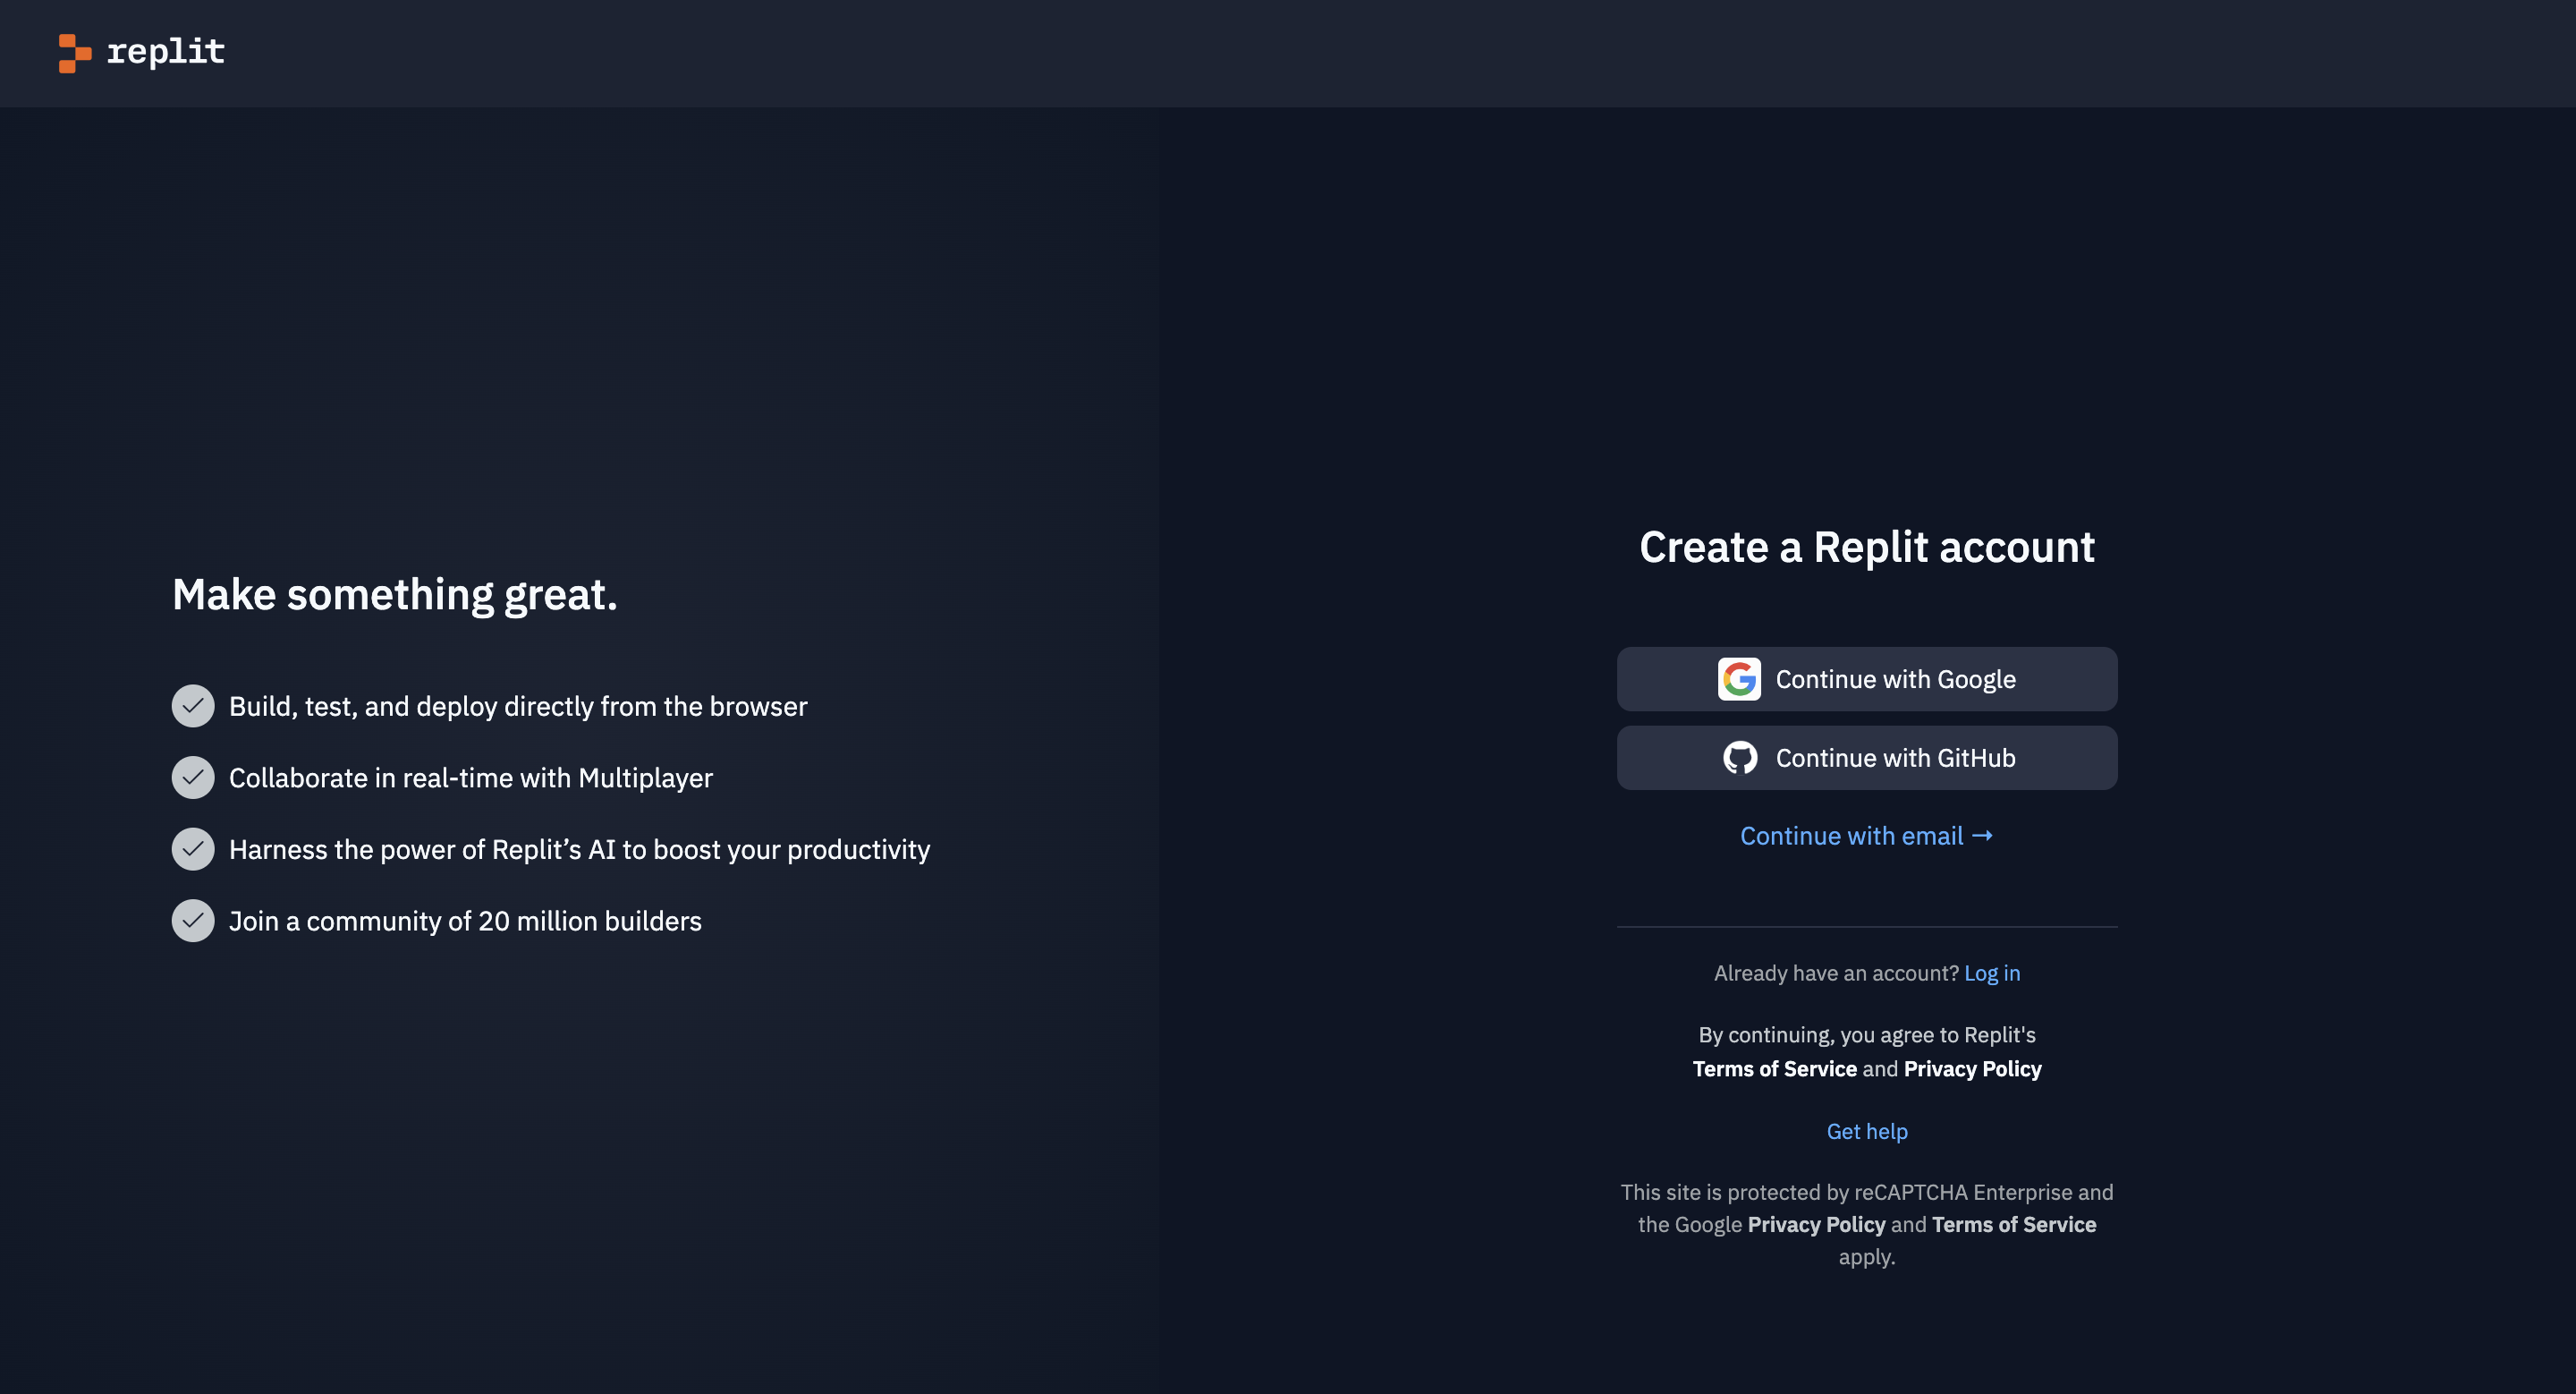
\includegraphics{./imgs/unidad_1/replit_signup.png}

}

\caption{Página de creación de cuenta de Replit}

\end{figure}%

\subsection{Creación de un nuevo
proyecto}\label{creaciuxf3n-de-un-nuevo-proyecto}

Una vez creada la cuenta e iniciado sesión, vamos a ver esta pantalla:

\begin{figure}[H]

{\centering 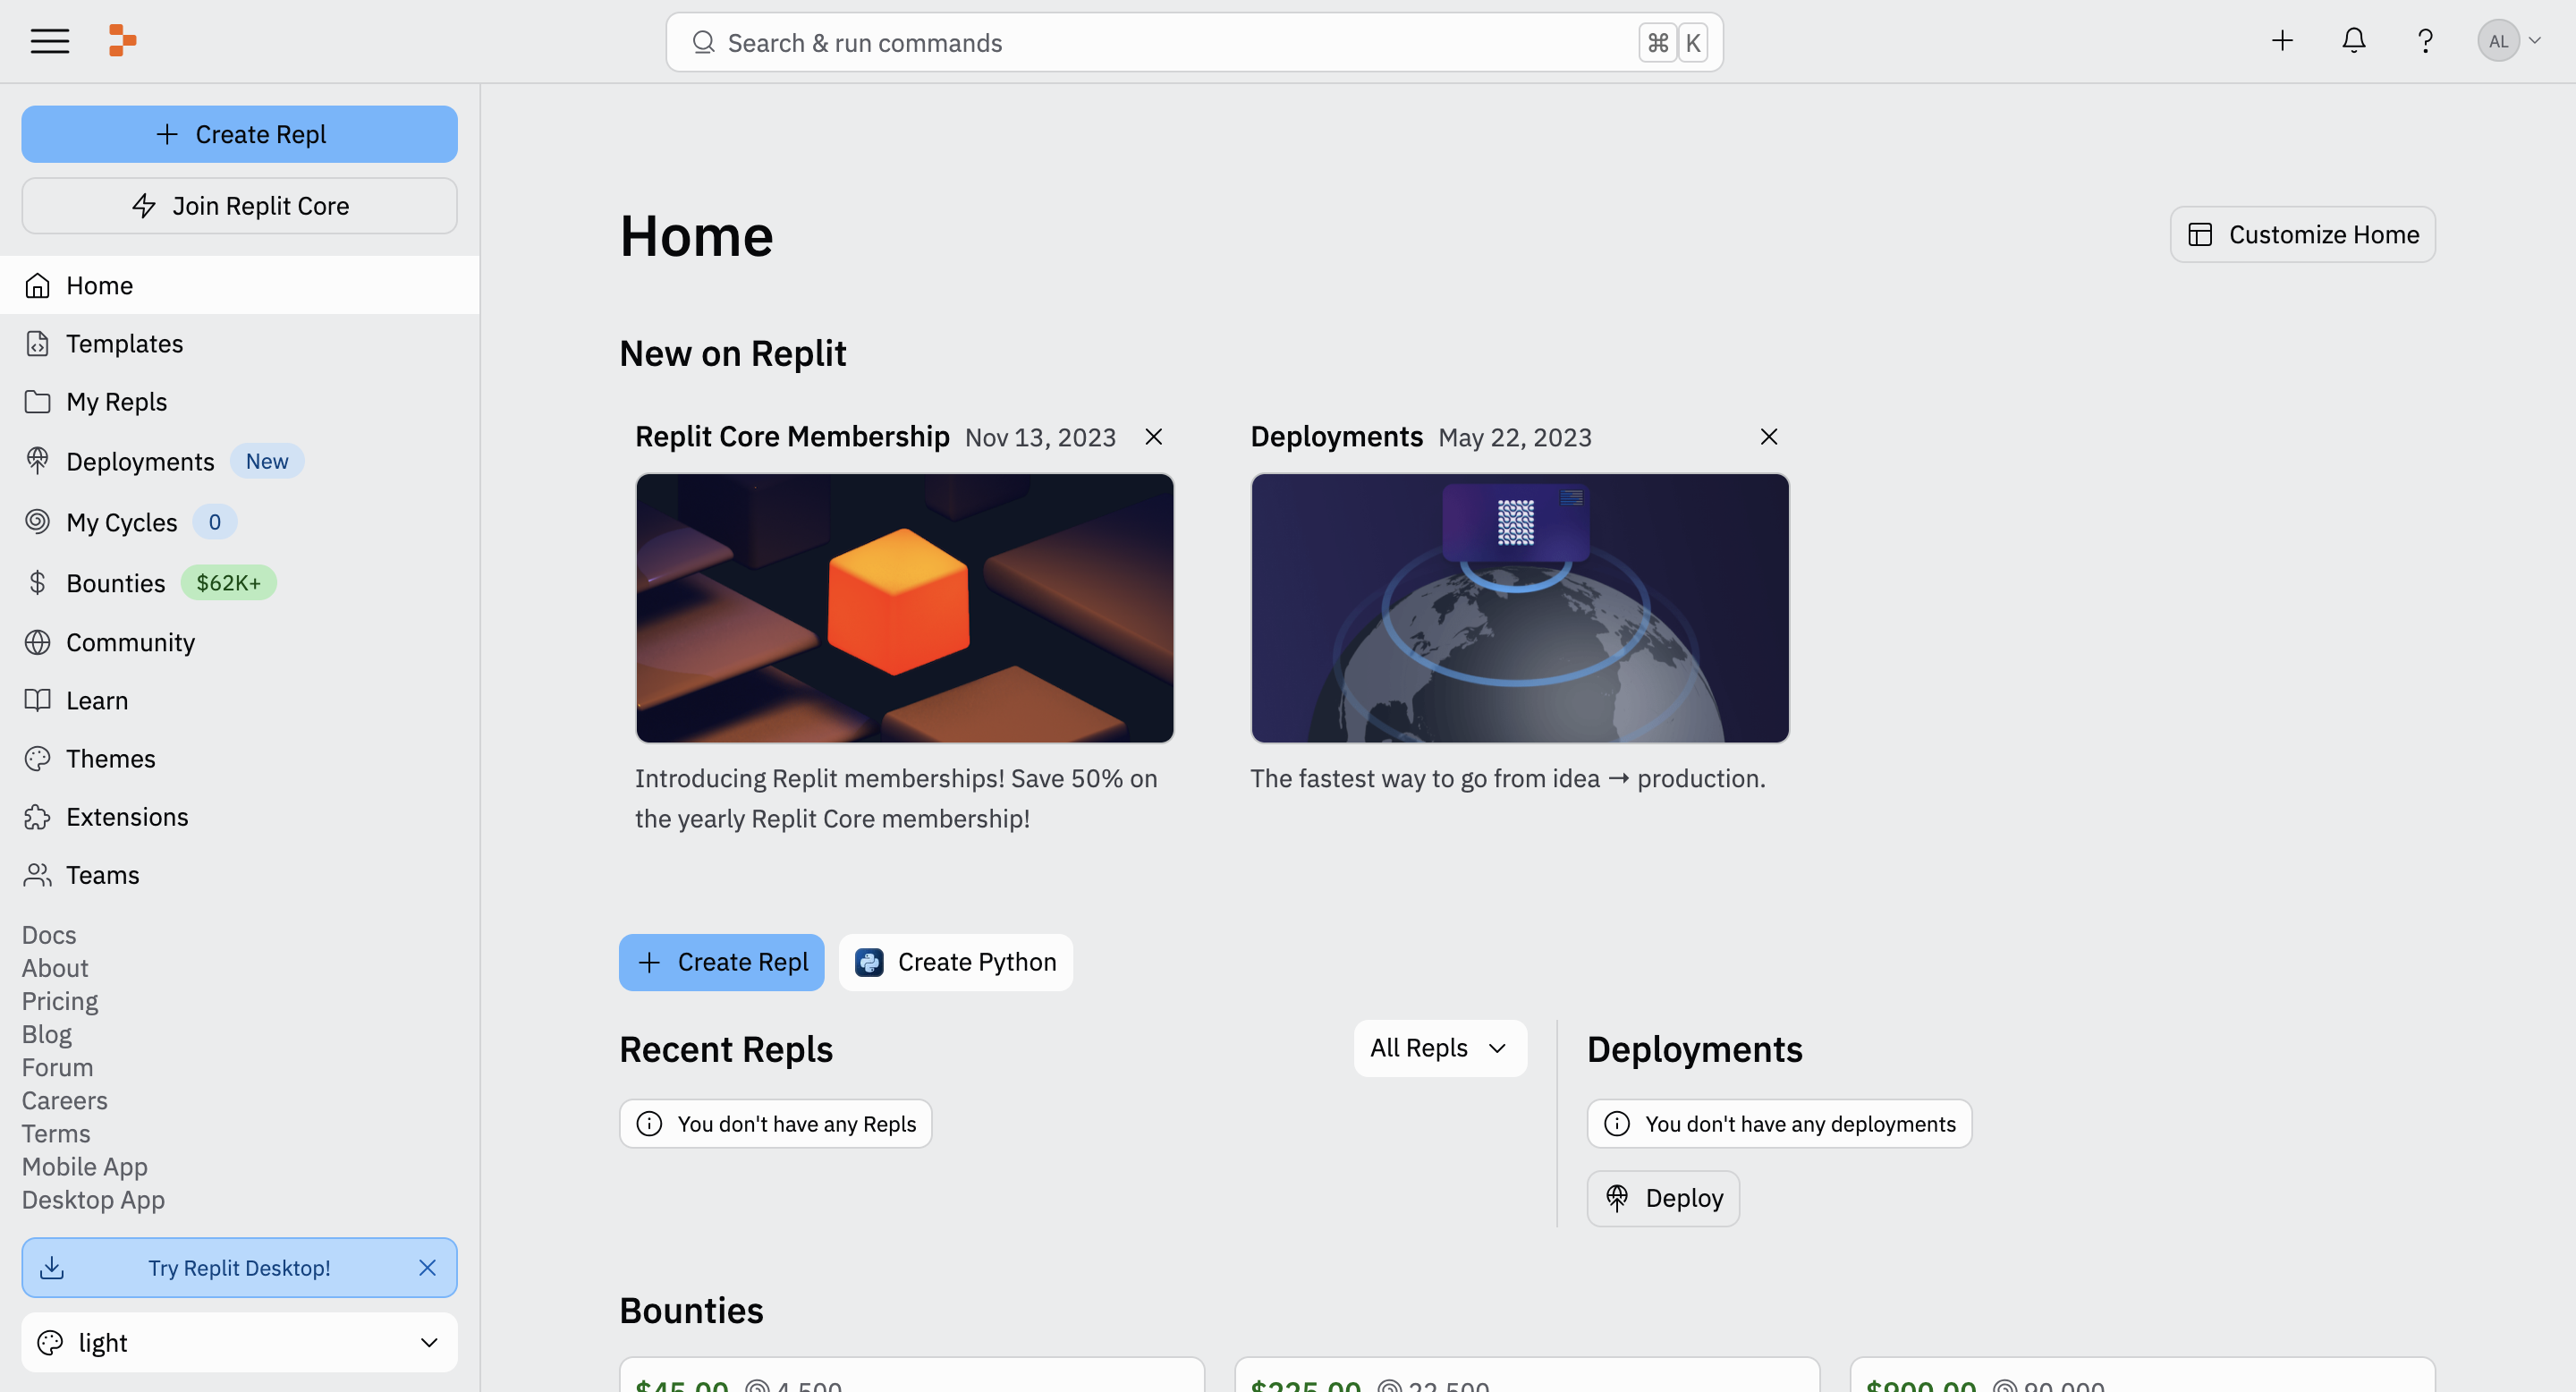
\includegraphics{./imgs/unidad_1/replit_home.png}

}

\caption{Home de Replit}

\end{figure}%

En la misma vamos a ver muchas opciones, pero la que nosotros nos
interesa es el botón de \texttt{+\ Create\ Repl}, que nos va a permitir
crear un nuevo proyecto.

\begin{figure}[H]

{\centering 
\includegraphics{./imgs/unidad_1/replit_create_repl.png}

}

\caption{Botón de creación de un nuevo proyecto en Replit}

\end{figure}%

Se va a abrir la siguiente ventana:
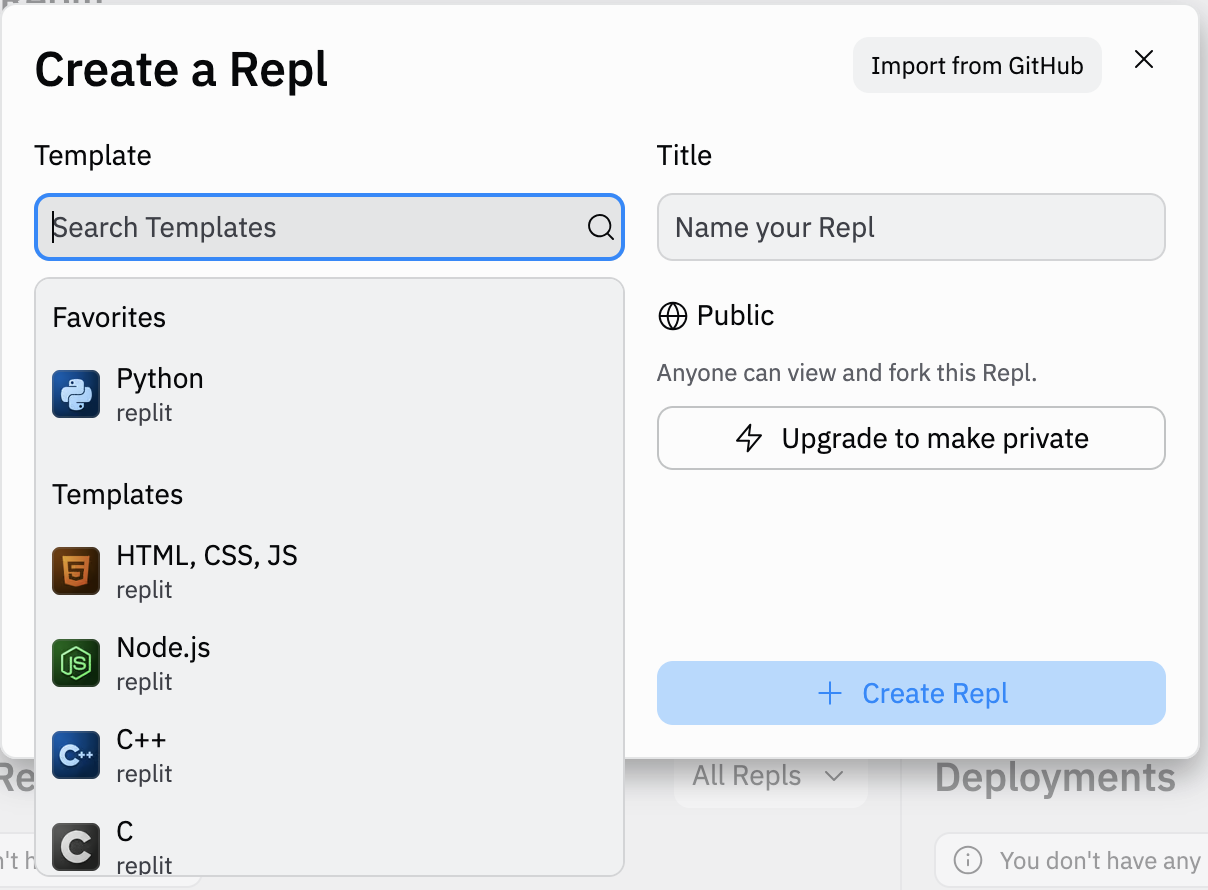
\includegraphics{./imgs/unidad_1/replit_create_repl2.png}

Donde vamos a buscar y elegir en ``Templates'' el lenguaje de
programación Python. Luego, vamos a asignarle un nombre y seleccionar
``Create repl''.\\
Se debería ver algo así:

\begin{figure}[H]

{\centering 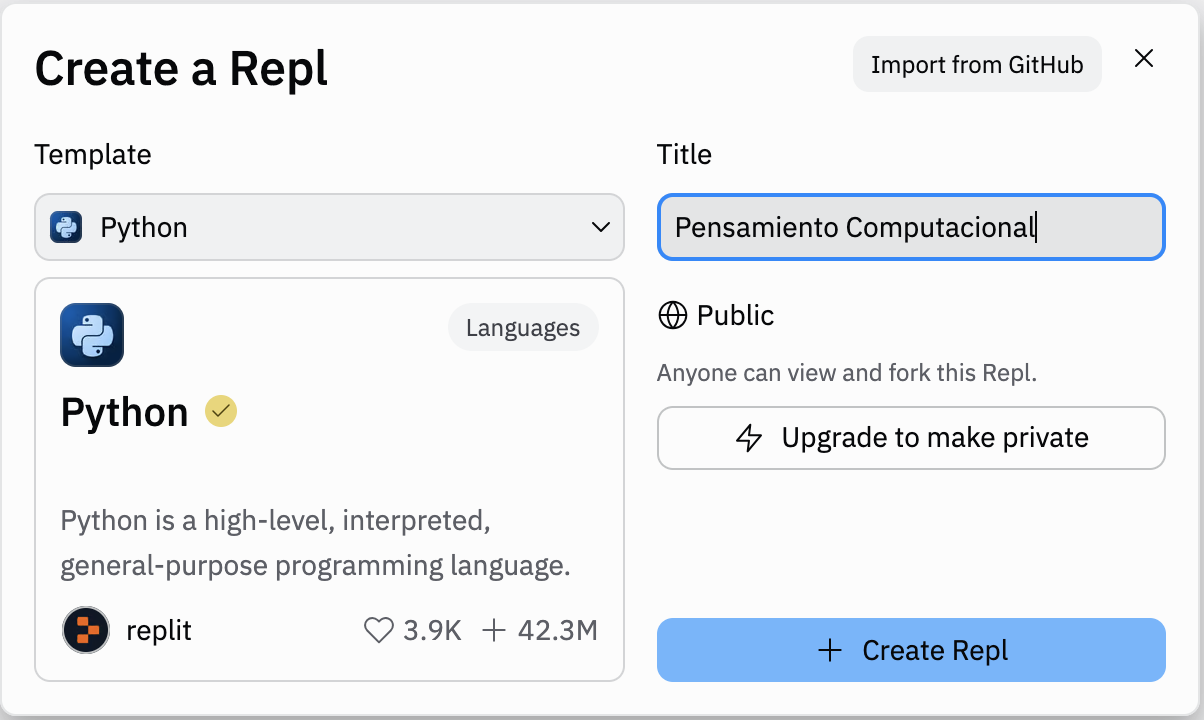
\includegraphics{./imgs/unidad_1/replit_create_repl3.png}

}

\caption{Ventana completa de creación de un nuevo proyecto en Replit}

\end{figure}%

\subsection{Uso del nuevo proyecto}\label{uso-del-nuevo-proyecto}

Los espacios o proyectos en replit se llaman \texttt{Workspace}, que
significa \texttt{espacio\ de\ trabajo}. En este espacio de trabajo
vamos a poder escribir código, ejecutarlo, y ver los resultados de la
ejecución.

Una vez creado el espacio de trabajo, se nos va a abrir una pantalla
donde vamos a ver varias cosas.

Inicialmente, tenemos en el centro el espacio de edición de código,
donde vamos a escribir nuestro programa.
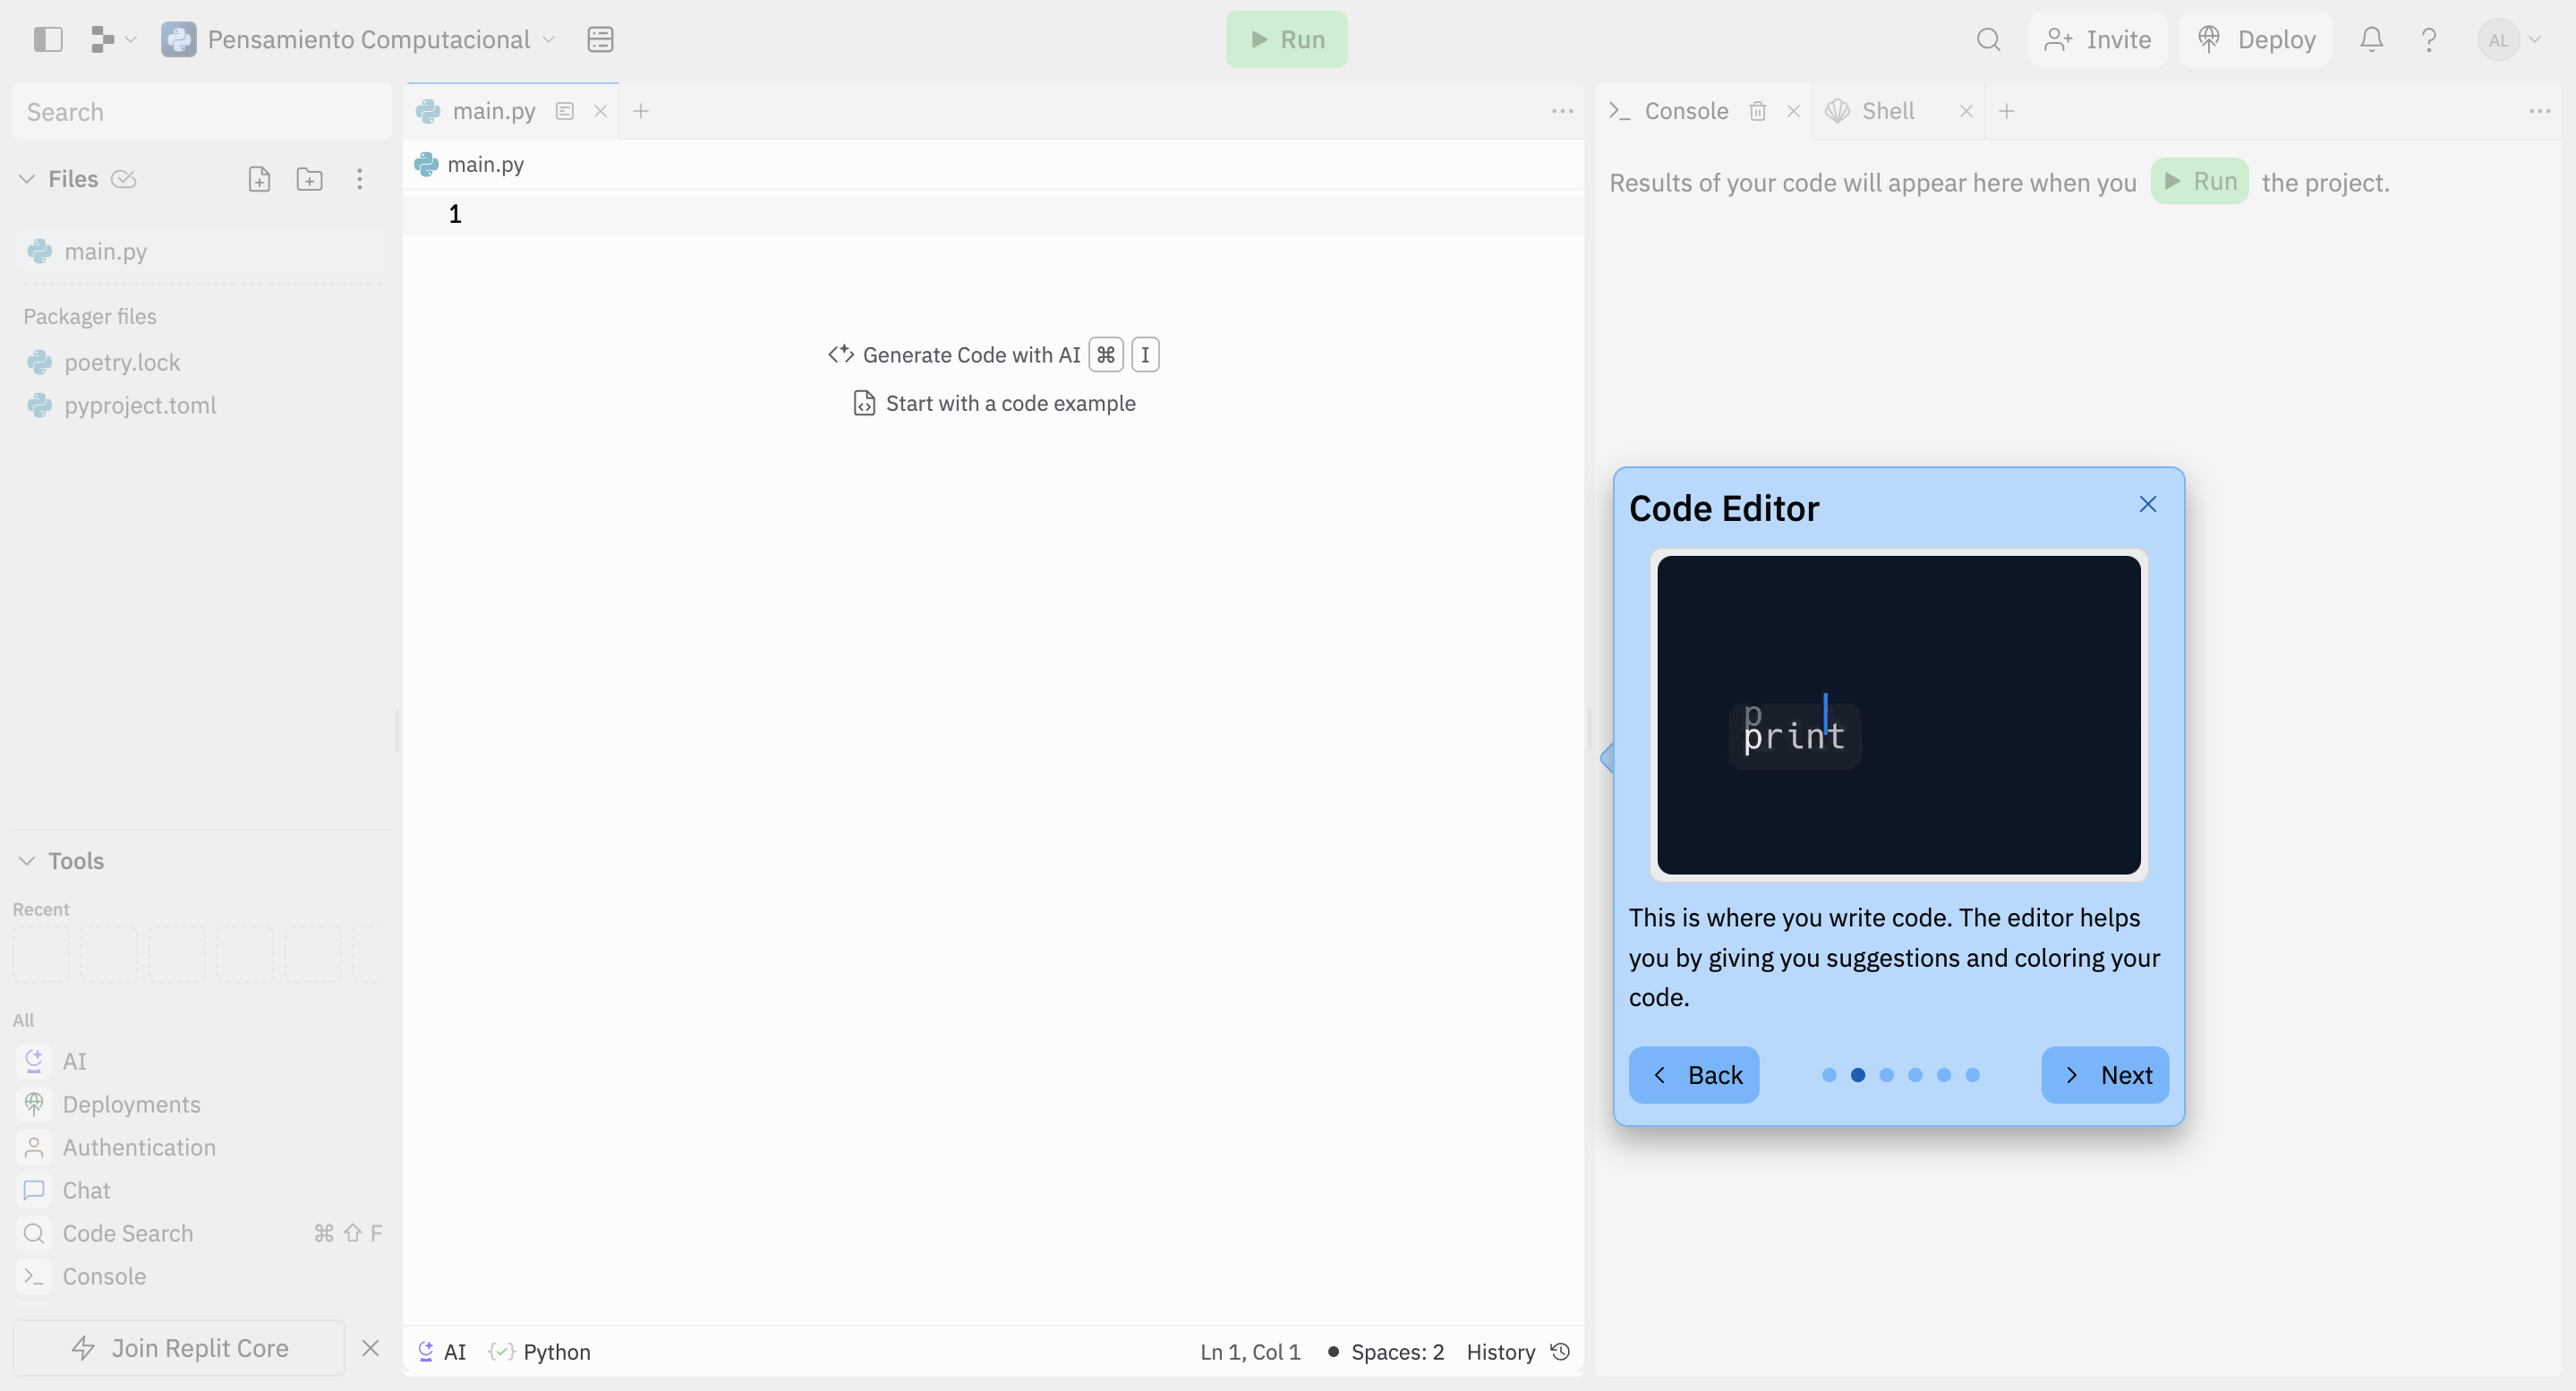
\includegraphics{./imgs/unidad_1/replit_workspace1.png}

En la parte superior, vamos a ver un botón de \texttt{Run}, que nos va a
permitir ejecutar el programa que escribimos.

\begin{figure}[H]

{\centering 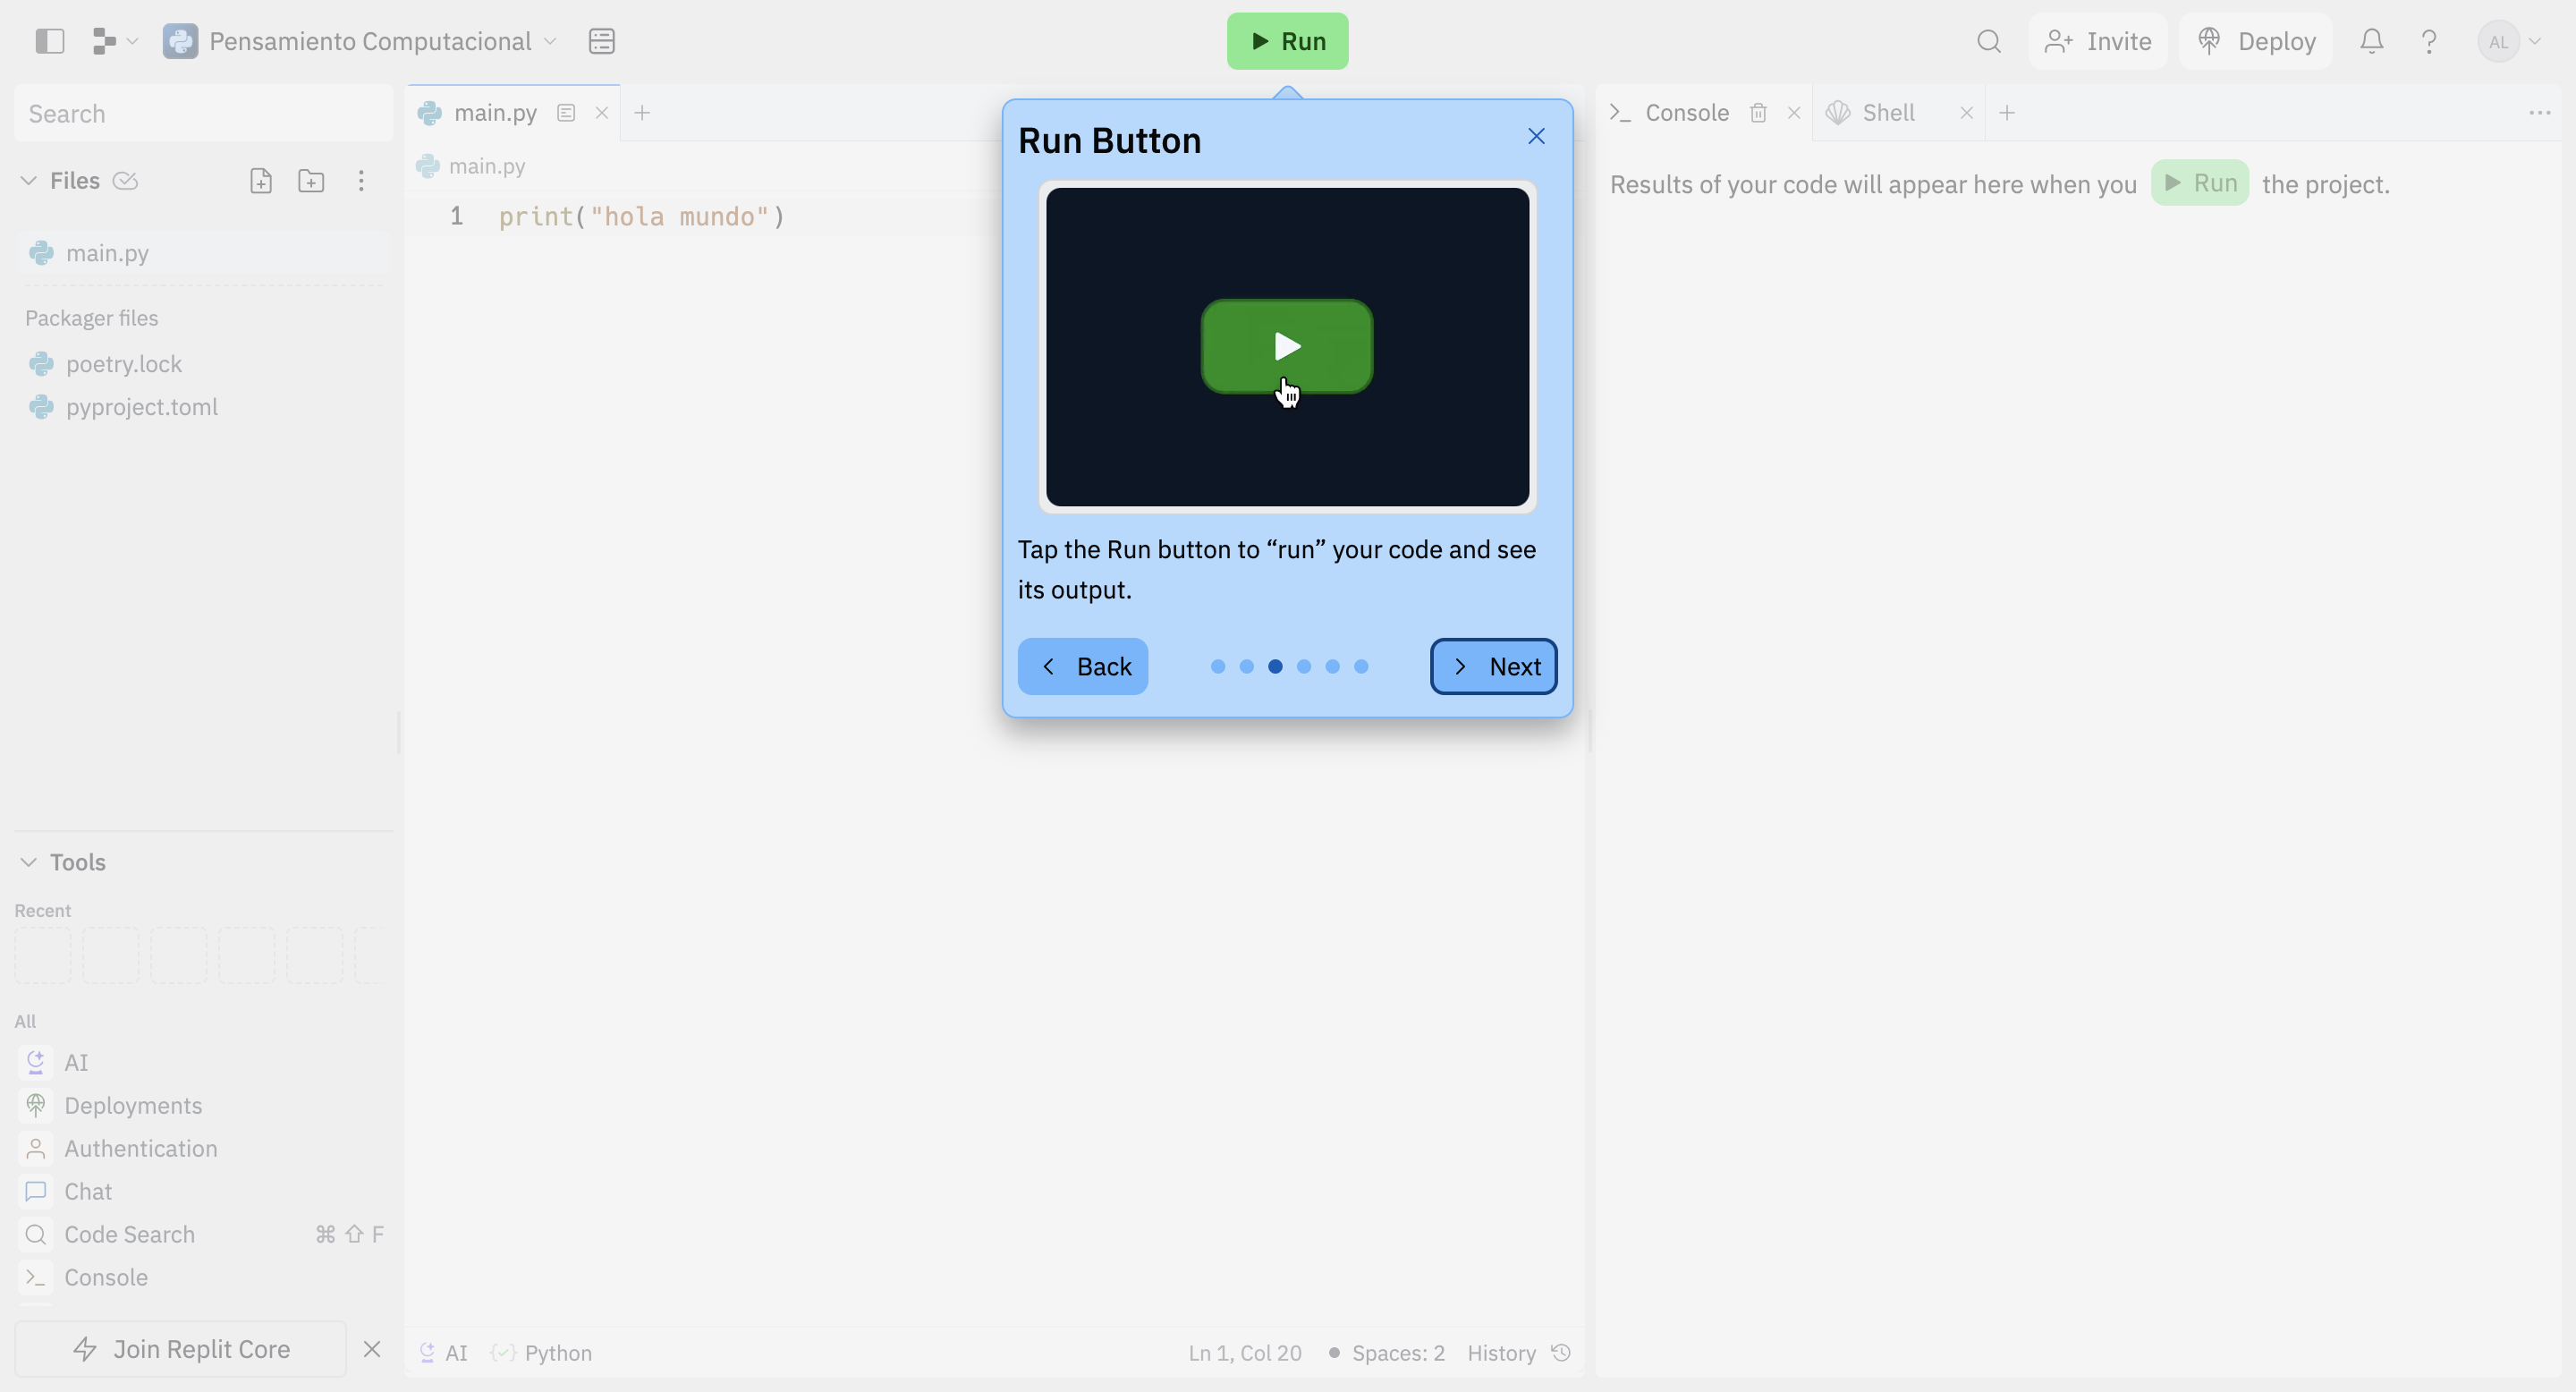
\includegraphics{./imgs/unidad_1/replit_workspace2.png}

}

\caption{Botón de ejecución de código}

\end{figure}%

En la parte derecha, vamos a ver el resultado de la ejecución del
programa. En este caso, como no escribimos nada, no hay nada para
mostrar.

\begin{figure}[H]

{\centering 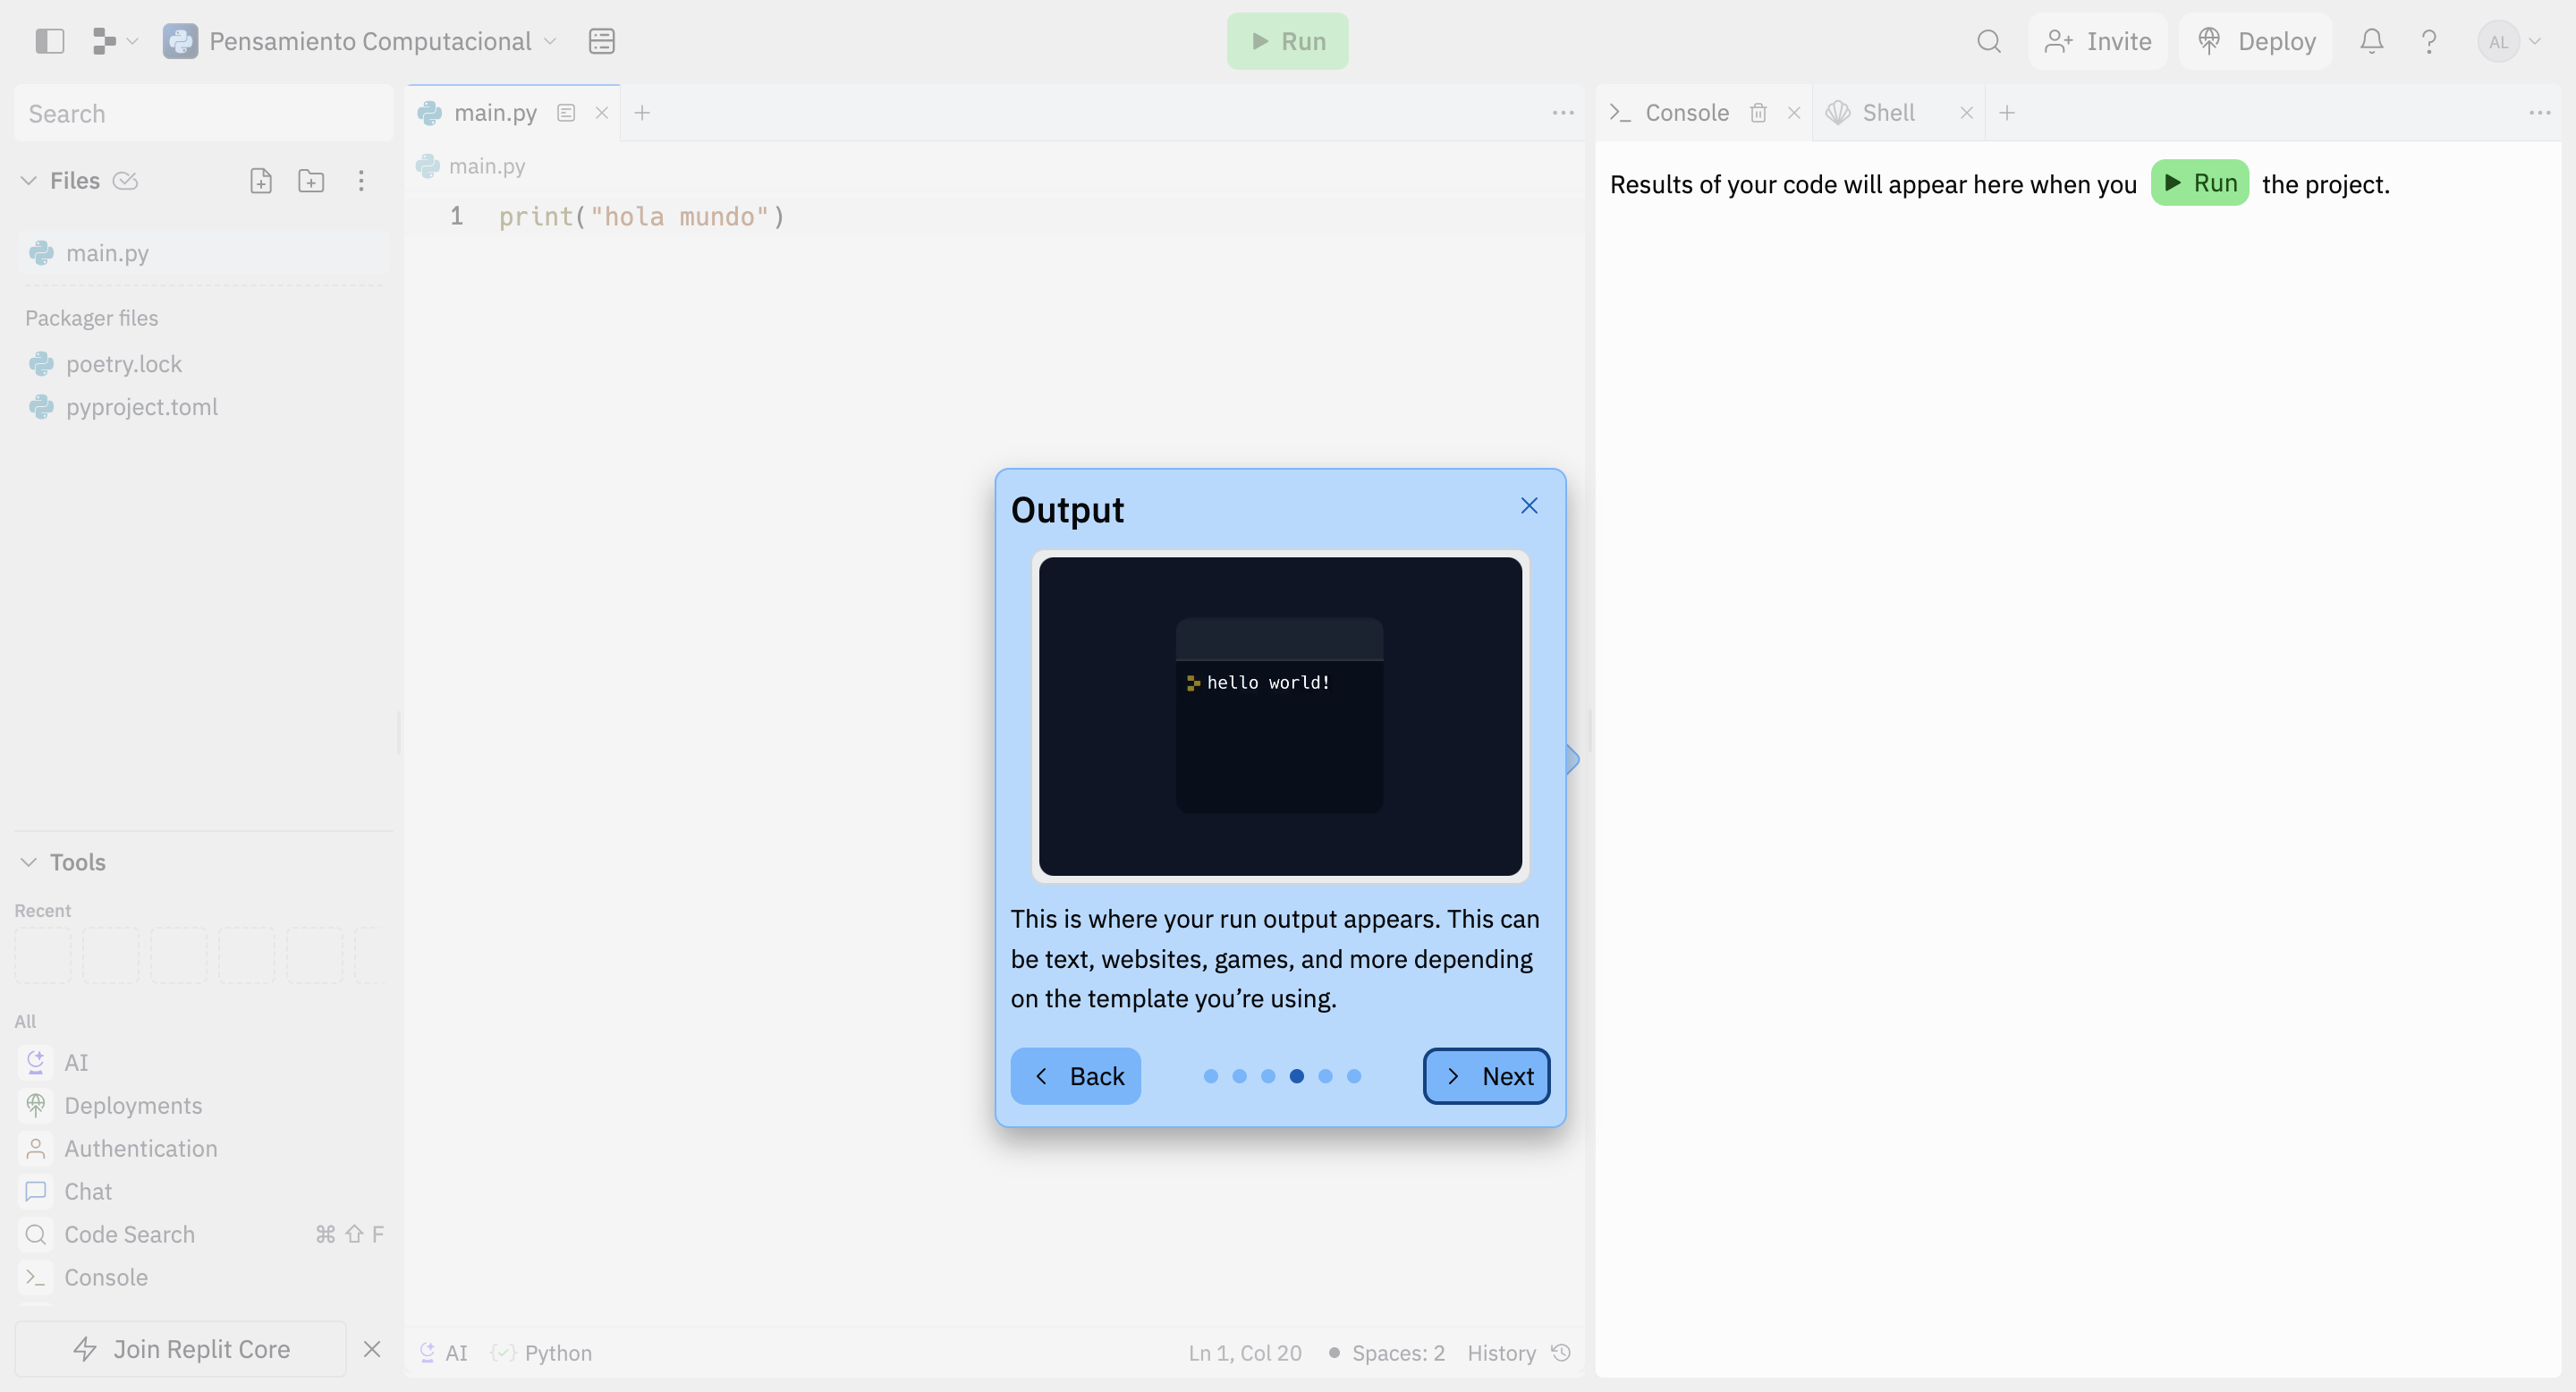
\includegraphics{./imgs/unidad_1/replit_workspace3.png}

}

\caption{Resultado de la ejecución de código}

\end{figure}%

Finalmente, en la parte izquierda vamos a tener el menú de archivos,
donde vamos a poder crear nuevos archivos, borrarlos, etc. También tiene
el acceso a otras herramientas que de momento no vamos a estar usando.

\begin{figure}[H]

{\centering 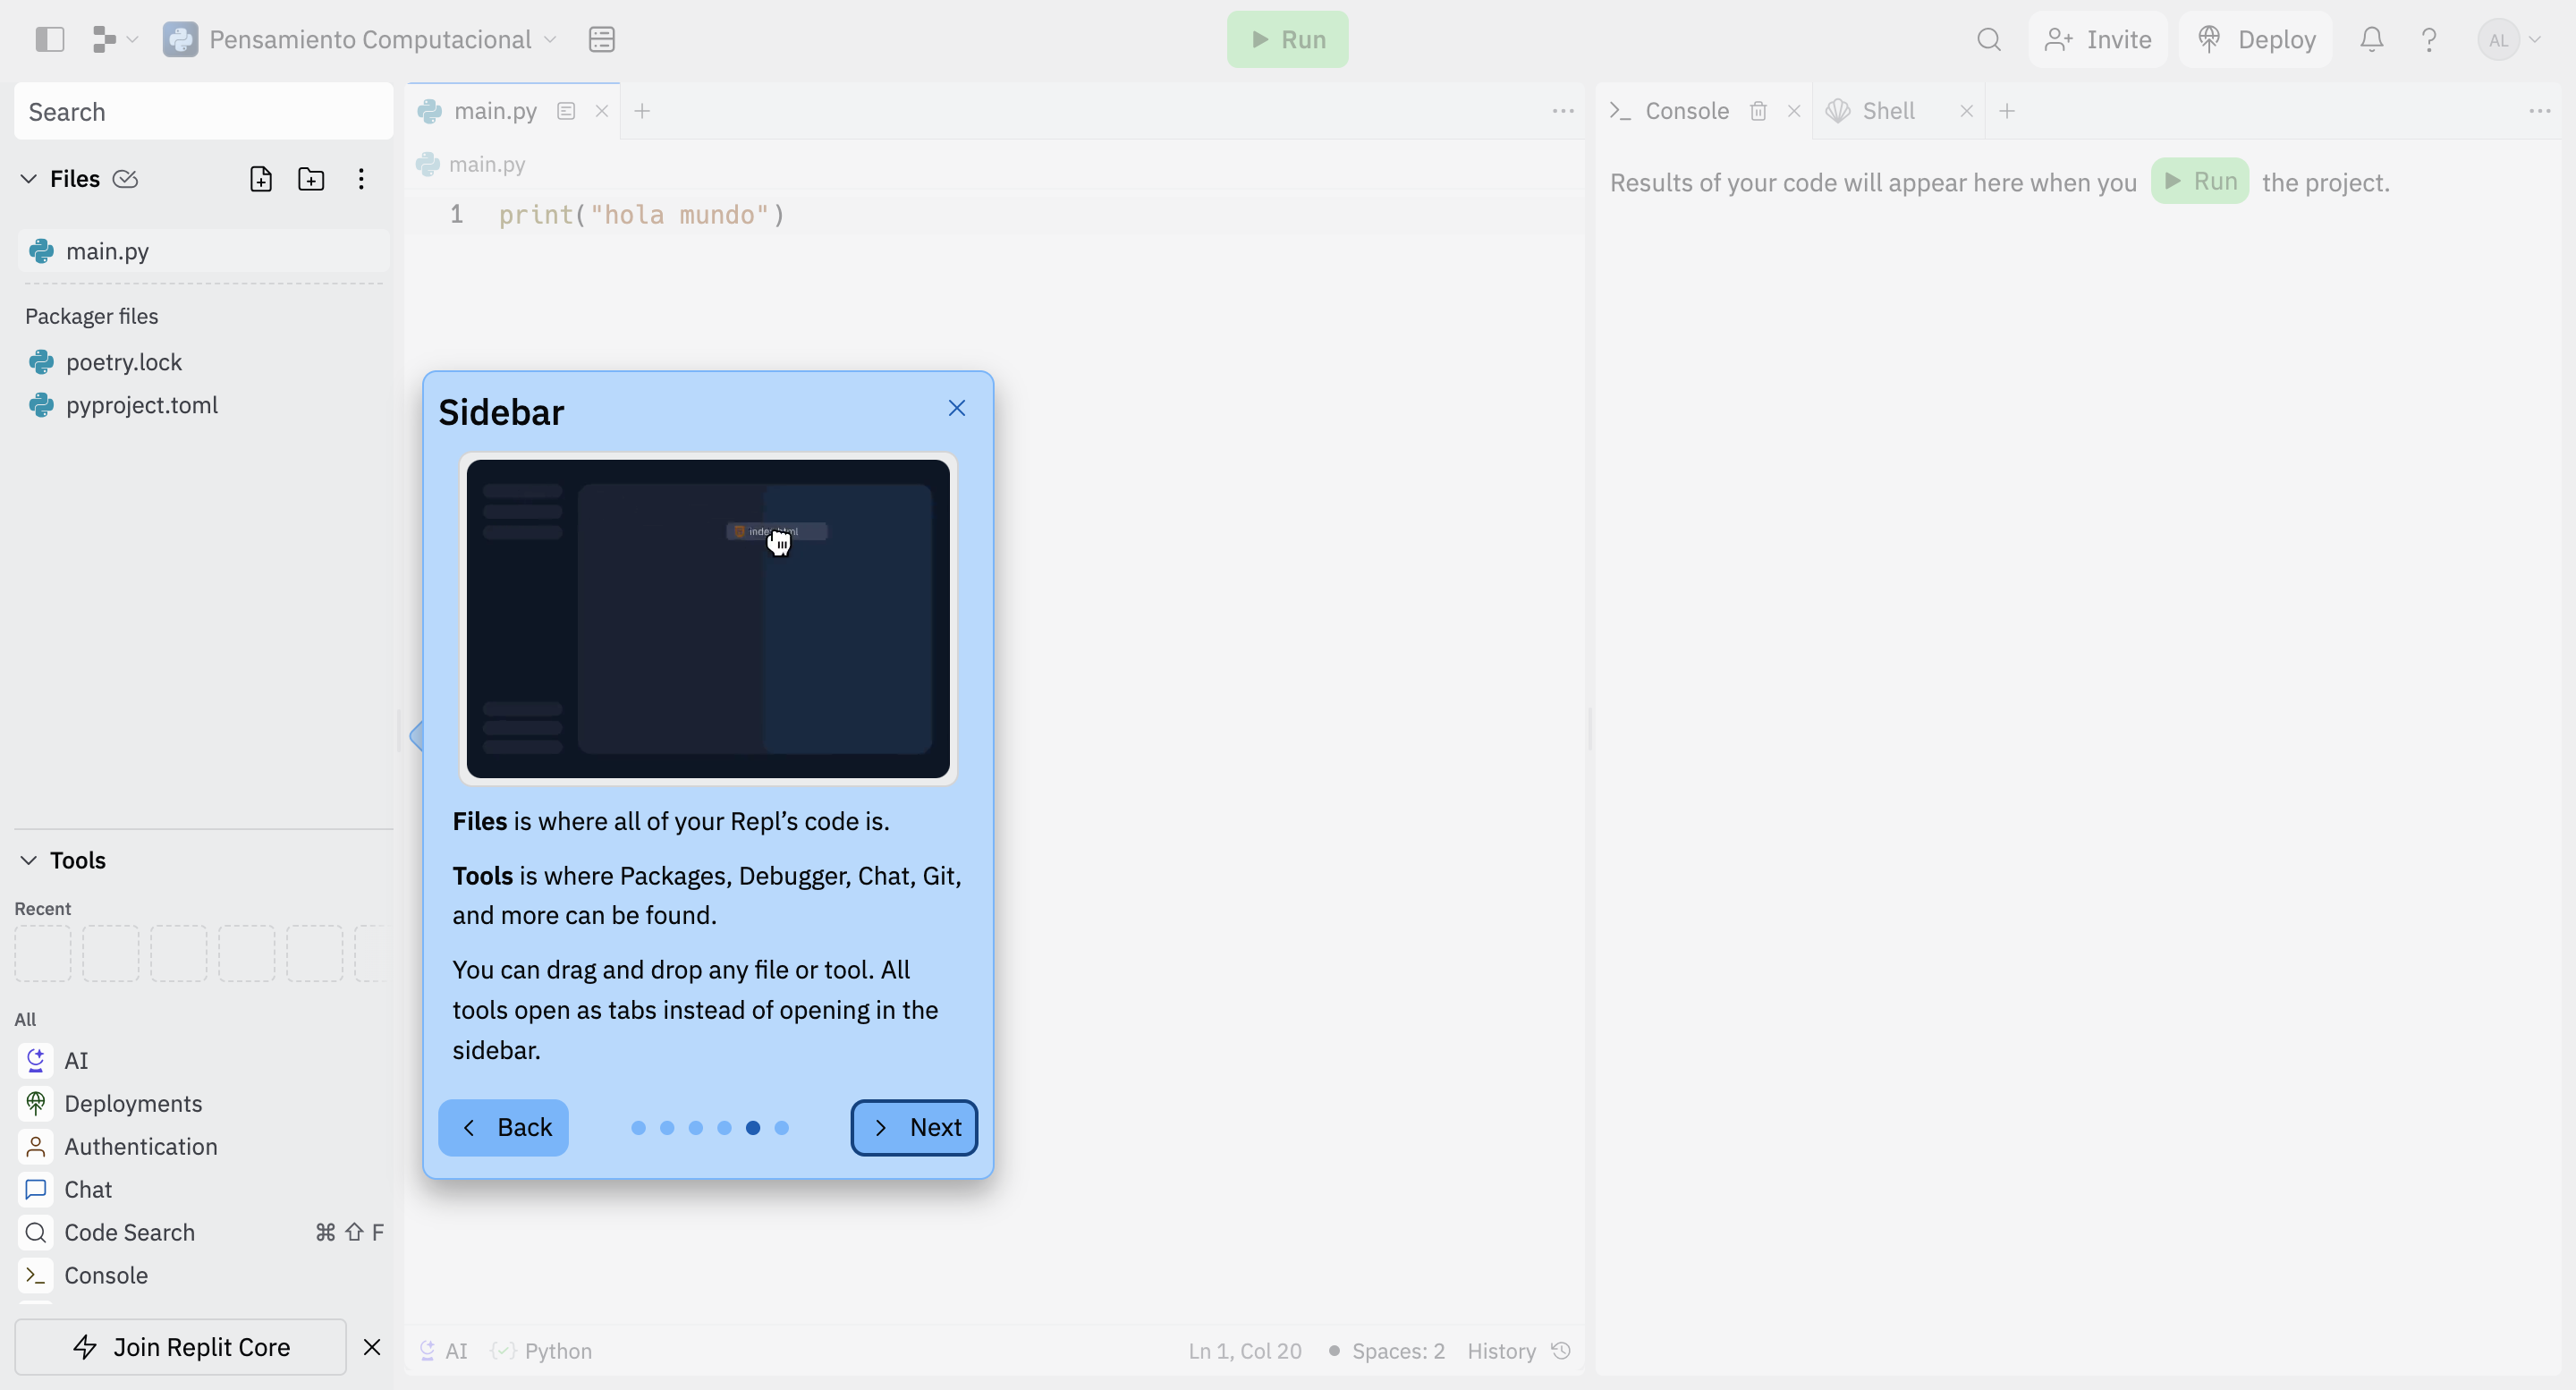
\includegraphics{./imgs/unidad_1/replit_workspace4.png}

}

\caption{Menú de archivos}

\end{figure}%

Vamos a ver que en el menú de archivos ya tenemos un archivo creado,
llamado \texttt{main.py}. Este archivo es el archivo principal de
nuestro programa, y es el que se ejecuta cuando presionamos el botón de
\texttt{Run}.\\
Si bien podemos tener otros archivos, el único que se ejecuta cuando
presionamos \texttt{Run} es \texttt{main.py}. Por lo tanto, es
importante que nuestro programa principal o lo que nosotros queremos
correr, esté en este archivo. Lo que podemos hacer, es crear otros
archivos para ir guardando nuestro código y ejercicios anteriores sin
necesidad de que se ejecuten cada vez que presionamos \texttt{Run}.

\begin{quote}
\textbf{¡Probemos el espacio de trabajo!} Vamos a escribir en el archivo
\texttt{main.py} el siguiente código: \texttt{print("Hola,\ Mundo!")}.
Luego, vamos a presionar el botón de \texttt{Run} y vamos a ver el
resultado en la parte derecha de la pantalla.
\end{quote}

¡Felicitaciones! Ya escribiste tu primer programa en Python.

\begin{tcolorbox}[enhanced jigsaw, bottomrule=.15mm, leftrule=.75mm, opacityback=0, colback=white, toprule=.15mm, bottomtitle=1mm, opacitybacktitle=0.6, rightrule=.15mm, left=2mm, arc=.35mm, coltitle=black, title=\textcolor{quarto-callout-note-color}{\faInfo}\hspace{0.5em}{}, breakable, toptitle=1mm, colframe=quarto-callout-note-color-frame, titlerule=0mm, colbacktitle=quarto-callout-note-color!10!white]

¿Lograste ver el resultado? ¿Qué pasa si presionás el botón de
\texttt{Run} varias veces seguidas?\\

\end{tcolorbox}

\bookmarksetup{startatroot}

\chapter{Tipos de Datos, Expresiones y
Funciones}\label{tipos-de-datos-expresiones-y-funciones}

\section{Sentencias Básicas}\label{sentencias-buxe1sicas}

En esta unidad vamos a centrarnos en la herramienta que vamos a emplear,
que es Python. Vamos a hacer un programa sencillo, interactuar con el
usuario y más.

\subsection{Flujo de Control de un
Programa}\label{flujo-de-control-de-un-programa}

El flujo de control de un programa es la forma en la que se ejecutan las
instrucciones de un programa. En Python, el flujo de control es
secuencial, es decir, se ejecutan las instrucciones una detrás de otra.

\textbf{Ejemplo:}

\begin{Shaded}
\begin{Highlighting}[]
\NormalTok{Esta línea se ejecutaría primero        ↓}
\NormalTok{Esta línea se ejecutaría después        ↓}
\NormalTok{Esta línea se ejecutaría a lo último    }
\end{Highlighting}
\end{Shaded}

En este curso, la comunicación de los programas con el mundo exterior se
realizará casi exclusivamente con el usuario por medio de la consola (o
terminal, la presentamos en la unidad anterior en el anexo de Replit).

\begin{tcolorbox}[enhanced jigsaw, bottomrule=.15mm, leftrule=.75mm, opacityback=0, colback=white, toprule=.15mm, bottomtitle=1mm, opacitybacktitle=0.6, rightrule=.15mm, left=2mm, arc=.35mm, coltitle=black, title=\textcolor{quarto-callout-warning-color}{\faExclamationTriangle}\hspace{0.5em}{¡Cuidado!}, breakable, toptitle=1mm, colframe=quarto-callout-warning-color-frame, titlerule=0mm, colbacktitle=quarto-callout-warning-color!10!white]

Esto no significa que todos los programas siempre se comuniquen con el
usuario para todo. Pensemos en las aplicaciones que usamos generalmente,
como instagram: imaginémonos si para cada acción que hiciéramos dentro
de la app la misma nos preguntara si queremos hacerlo o no:\\

\textbf{- ``¿Estás seguro/a de que querés iniciar sesión?''}\\
\textbf{- ``¿Estás seguro/a de que querés traer tu nombre de usuario
para mostrarse en el perfil?''}\\
\textbf{- ``¿Estás seguro/a de que querés traer tu foto de usuario para
mostrarse en el perfil?''}\\

Sería extremadamente molesto. Uno simplemente inicia sesión, y hay un
montón de cosas y procesos que se ejecutan uno detrás de otro,
automáticamente.\\

Hay cosas que no necesitan de la interacción del usuario. Nosotros nos
vamos a centrar en la interacción con el usuario en gran parte del
curso, pero no es lo único que se puede hacer. Los programas pueden
comunicarse con otros programas y las partes de un mismo programa pueden
comunicarse con otras partes del mismo programa.~ Más adelante vamos a
ver un poco más de esta diferencia.

\end{tcolorbox}

\subsection{Valores y Tipos}\label{valores-y-tipos}

Si tenemos la operación \texttt{7\ *\ 5}, sabemos que el resultado es
\texttt{35}. Decimos que tanto \texttt{7}, \texttt{5} como \texttt{35}
son \emph{valores}. En los lenguajes de programación, cada valor tiene
un \emph{tipo}.

En este caso, \texttt{7}, \texttt{5} y \texttt{35} son \emph{enteros} (o
\emph{integers} en inglés). En Python, los enteros se representan con el
tipo \texttt{int}.

Python tiene dos tipos de datos numéricos: - número enteros - números de
punto flotante

Los \textbf{números enteros} representan un valor entero exacto, como
\texttt{42}, \texttt{0}, \texttt{-5} o \texttt{10000}.\\
Los \textbf{números de punto flotante} tienen una parte fraccionaria,
como \texttt{3.14159}, \texttt{1.0} o \texttt{0.0}.

Según los operandos (los valores que se operan) y el operador (el
símbolo que indica la operación), el resultado puede ser de un tipo u
otro. Por ejemplo, si tenemos \texttt{7\ /\ 5}, el resultado es
\texttt{1.4}, que es un número de punto flotante. Si tenemos
\texttt{7\ +\ 5}, el resultado es \texttt{12}, que es un número entero.

\begin{Shaded}
\begin{Highlighting}[]
\DecValTok{1} \OperatorTok{+} \DecValTok{2}
\end{Highlighting}
\end{Shaded}

\begin{verbatim}
3
\end{verbatim}

Vamos a elegir usar enteros cada vez que necesitemos recordar, almacenar
o representar un valor exacto, como pueden ser por ejemplo: la cantidad
de alumnos, cuántas veces repetimos una operación, un número de
documento, etc.\\
Vamos a elegir usar números de punto flotante cada vez que necesitemos
recordar, almacenar o representar un valor aproximado, como pueden ser
por ejemplo: la altura o el peso de una persona, la temperatura de un
día, una distancia recorrida, etc.

\begin{Shaded}
\begin{Highlighting}[]
\FloatTok{0.1} \OperatorTok{+} \FloatTok{0.2}
\end{Highlighting}
\end{Shaded}

\begin{verbatim}
0.30000000000000004
\end{verbatim}

Como vemos, cuando hay números de punto flotante, el resultado es
aproximado. \texttt{0.1\ +\ 0.2} nos debería dar \texttt{0.3}, pero nos
da \texttt{0.30000000000000004}. Esto es porque los números de punto
flotante son aproximados, y no pueden representar todos los valores de
forma exacta. Esto es algo que vamos a tener que tener en cuenta cuando
trabajemos con números de punto flotante.

\begin{tcolorbox}[enhanced jigsaw, bottomrule=.15mm, leftrule=.75mm, opacityback=0, colback=white, toprule=.15mm, bottomtitle=1mm, opacitybacktitle=0.6, rightrule=.15mm, left=2mm, arc=.35mm, coltitle=black, title=\textcolor{quarto-callout-note-color}{\faInfo}\hspace{0.5em}{Uso de punto}, breakable, toptitle=1mm, colframe=quarto-callout-note-color-frame, titlerule=0mm, colbacktitle=quarto-callout-note-color!10!white]

Notemos que para representar números de punto flotante, usamos el punto
(\texttt{.}) y no la coma (\texttt{,}). Esto es porque en Python, la
coma se usa para separar valores, como vamos a ver más adelante.

\end{tcolorbox}

Además de efectuar operaciones matemáticas, Python nos permite trabajar
con porciones de texto, que se llaman \textbf{cadenas} (o \emph{strings}
en inglés). Las cadenas se representan con el tipo \texttt{str}.\\
Las cadenas se escriben entre comillas simples
(\texttt{\textquotesingle{}}) o dobles (\texttt{"}).

\begin{Shaded}
\begin{Highlighting}[]
\BuiltInTok{print}\NormalTok{( }\StringTok{"¡Hola!"}\NormalTok{ )}
\end{Highlighting}
\end{Shaded}

\begin{verbatim}
¡Hola!
\end{verbatim}

\begin{Shaded}
\begin{Highlighting}[]
\BuiltInTok{print}\NormalTok{( }\StringTok{\textquotesingle{}¡Hola!\textquotesingle{}}\NormalTok{ )}
\end{Highlighting}
\end{Shaded}

\begin{verbatim}
¡Hola!
\end{verbatim}

Las cadenas también tienen operaciones disponibles, como por ejemplo la
concatenación, que es la unión de dos cadenas en una sola. Esto se hace
con el operador \texttt{+}.

\begin{Shaded}
\begin{Highlighting}[]
\BuiltInTok{print}\NormalTok{( }\StringTok{"¡Hola!"} \OperatorTok{+} \StringTok{" ¿Cómo estás?"}\NormalTok{ )}
\end{Highlighting}
\end{Shaded}

\begin{verbatim}
¡Hola! ¿Cómo estás?
\end{verbatim}

Vamos a ver más de estas operaciones más adelante.

\subsection{Variables}\label{variables}

Python nos permite asignarle un nombre a un valor, de forma tal que
podamos ``recordarlo'' y usarlo más adelante. A esto se le llama
\textbf{asignación}.\\
Estos nombres se llaman \textbf{variables}, y son espacios donde podemos
almacenar valores.\\

La asignación se hace con el operador \texttt{=} de la siguiente forma:
\texttt{\textless{}nombre\textgreater{}\ =\ \textless{}valor\ o\ expresion\textgreater{}}.

\textbf{Ejemplos:}

\begin{Shaded}
\begin{Highlighting}[]
\NormalTok{x }\OperatorTok{=} \DecValTok{5}
\end{Highlighting}
\end{Shaded}

\begin{Shaded}
\begin{Highlighting}[]
\NormalTok{y }\OperatorTok{=}\NormalTok{ x }\OperatorTok{+} \DecValTok{2}
\end{Highlighting}
\end{Shaded}

\begin{Shaded}
\begin{Highlighting}[]
\BuiltInTok{print}\NormalTok{(y)}
\end{Highlighting}
\end{Shaded}

\begin{verbatim}
7
\end{verbatim}

\begin{Shaded}
\begin{Highlighting}[]
\BuiltInTok{print}\NormalTok{(y }\OperatorTok{*} \DecValTok{2}\NormalTok{)}
\end{Highlighting}
\end{Shaded}

\begin{verbatim}
14
\end{verbatim}

\begin{Shaded}
\begin{Highlighting}[]
\NormalTok{lenguaje }\OperatorTok{=} \StringTok{"Python"}

\NormalTok{texto }\OperatorTok{=} \StringTok{"Estoy programando en "} \OperatorTok{+}\NormalTok{ lenguaje}
\BuiltInTok{print}\NormalTok{(texto)}
\end{Highlighting}
\end{Shaded}

\begin{verbatim}
Estoy programando en Python
\end{verbatim}

En este ejemplo, creamos las siguientes variables:

\begin{itemize}
\tightlist
\item
  x
\item
  y
\item
  lenguaje
\item
  texto
\end{itemize}

y las asociamos a los valores 5, 7, ``Python'' y ``Estoy programando en
Python'' respectivamente. Luego podemos usar esas variables como parte
de cualquier expresión, y en el momento de evaluarla, Python reemplazará
las variables por su valor asociado.

\begin{tcolorbox}[enhanced jigsaw, bottomrule=.15mm, leftrule=.75mm, opacityback=0, colback=white, toprule=.15mm, bottomtitle=1mm, opacitybacktitle=0.6, rightrule=.15mm, left=2mm, arc=.35mm, coltitle=black, title=\textcolor{quarto-callout-note-color}{\faInfo}\hspace{0.5em}{Variables y Constantes}, breakable, toptitle=1mm, colframe=quarto-callout-note-color-frame, titlerule=0mm, colbacktitle=quarto-callout-note-color!10!white]

Si el dato es inmutable (no puede cambiar) durante la ejecución del
programa, se dice que ese dato es una \textbf{constante}. Si tiene la
habilidad de cambiar, se dice que es una variable. En Python, todas las
variables son mutables, es decir, pueden cambiar su valor durante la
ejecución del programa.\\
Y no sólo pueden cambiar su valor, sino también su tipo:
\texttt{x\ =\ 5} y \texttt{x\ =\ "Hola"} son dos asignaciones válidas, y
se pueden hacer una debajo de la otra:

\begin{Shaded}
\begin{Highlighting}[]
\NormalTok{x }\OperatorTok{=} \DecValTok{5}
\NormalTok{x }\OperatorTok{=} \StringTok{"Hola"}
\BuiltInTok{print}\NormalTok{(x)}
\end{Highlighting}
\end{Shaded}

\begin{verbatim}
Hola
\end{verbatim}

\end{tcolorbox}

\begin{tcolorbox}[enhanced jigsaw, bottomrule=.15mm, leftrule=.75mm, opacityback=0, colback=white, toprule=.15mm, bottomtitle=1mm, opacitybacktitle=0.6, rightrule=.15mm, left=2mm, arc=.35mm, coltitle=black, title=\textcolor{quarto-callout-warning-color}{\faExclamationTriangle}\hspace{0.5em}{Nombres de Variables}, breakable, toptitle=1mm, colframe=quarto-callout-warning-color-frame, titlerule=0mm, colbacktitle=quarto-callout-warning-color!10!white]

No se puede usar el mismo nombre para dos datos diferentes a la vez; una
variable puede referenciar un sólo dato por vez. Si se usa un mismo
nombre para un dato diferente, se pierde la referencia al dato
anterior.\\

\end{tcolorbox}

\subsection{Funciones}\label{funciones}

Para poder realizar algunas operaciones particulares, necesitamos
introducir el concepto de \emph{función}. Una función es un bloque de
código que se ejecuta cuando se la llama.\\
Es un fragmento de programa que permite efectuar una operación
determinada. \texttt{abs}, \texttt{print}, \texttt{max} son ejemplos de
funciones de Python: \texttt{abs}permite calcular el valor absoluto de
un número, \texttt{print} permite mostrar un valor por pantalla y
\texttt{max} permite calcular el máximo entre dos valores.\\

Una función puede recibir 0 o más \emph{parámetros} o \emph{argumentos},
que son valores que se le pasan a la función entre paréntesis y
separados por comas, para que los use.\\

\begin{Shaded}
\begin{Highlighting}[]
\BuiltInTok{abs}\NormalTok{(}\OperatorTok{{-}}\DecValTok{5}\NormalTok{)}
\end{Highlighting}
\end{Shaded}

\begin{verbatim}
5
\end{verbatim}

\begin{Shaded}
\begin{Highlighting}[]
\BuiltInTok{print}\NormalTok{(}\StringTok{"¡Hola!"}\NormalTok{)}
\end{Highlighting}
\end{Shaded}

\begin{verbatim}
¡Hola!
\end{verbatim}

\begin{Shaded}
\begin{Highlighting}[]
\BuiltInTok{max}\NormalTok{(}\DecValTok{5}\NormalTok{, }\DecValTok{7}\NormalTok{)}
\end{Highlighting}
\end{Shaded}

\begin{verbatim}
7
\end{verbatim}

La función recibe los parámetros, efectúa una operación y devuelve un
\emph{resultado}.

Python viene equipado de muchas funciones predefinidas, pero nosotros
como programadores debemos ser capaces de escribir nuevas instrucciones
para la computadora. Las grandes aplicaciones como el correo
electrónico, navegación web, chat, juegos, etc. no son más que grandes
programas implementados introduciendo nuevas funciones a la máquina,
escritas por uno o más programadores.

\begin{figure}[H]

{\centering 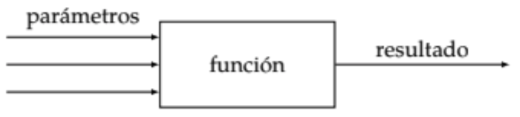
\includegraphics{./imgs/unidad_2/funcion.png}

}

\caption{Una función recibe parámetros y devuelve un resultado}

\end{figure}%

\begin{tcolorbox}[enhanced jigsaw, bottomrule=.15mm, leftrule=.75mm, opacityback=0, colback=white, toprule=.15mm, bottomtitle=1mm, opacitybacktitle=0.6, rightrule=.15mm, left=2mm, arc=.35mm, coltitle=black, title=\textcolor{quarto-callout-note-color}{\faInfo}\hspace{0.5em}{Python es Case Sensitive}, breakable, toptitle=1mm, colframe=quarto-callout-note-color-frame, titlerule=0mm, colbacktitle=quarto-callout-note-color!10!white]

Python es Case Sensitive, es decir, distingue entre mayúsculas y
minúsculas.\\
Es muy importante respetar mayúsculas y minúsculas: PRINT() o prINT() no
serán reconocidas. Esto aplica para todo lo que escribamos en nuestros
programas.

\end{tcolorbox}

Si queremos crear una función que nos devuelva un saludo a Lucia cada
vez que se la llama, debemos ingresar el siguiente conjunto de líneas en
Python:

\begin{Shaded}
\begin{Highlighting}[]
\KeywordTok{def}\NormalTok{ saludar\_lucia():}
  \ControlFlowTok{return} \StringTok{"Hola, Lucia!"}
\end{Highlighting}
\end{Shaded}

Varias cosas a notar del código:

\begin{enumerate}
\def\labelenumi{\arabic{enumi}.}
\tightlist
\item
  \texttt{saludar\_lucia} es el nombre de la función. Podría ser
  cualquier otro nombre, pero es una buena práctica que el nombre de la
  función describa lo que hace.\\
\item
  \texttt{def} es una palabra clave que indica que estamos definiendo
  una función.\\
\item
  \texttt{return} indica el valor que devuelve la función. Es decir, el
  \emph{resultado}. Puede devolverse una sola cosa, como en este caso, o
  varias cosas separadas por comas.\\
\item
  La sangría (el espacio inicial) en el renglón 2 le indica a Python que
  estamos dentro del \emph{cuerpo} de la función. El \emph{cuerpo} de la
  función es el bloque de código que se ejecuta cuando se llama a la
  misma.\\
\end{enumerate}

\begin{tcolorbox}[enhanced jigsaw, bottomrule=.15mm, leftrule=.75mm, opacityback=0, colback=white, toprule=.15mm, bottomtitle=1mm, opacitybacktitle=0.6, rightrule=.15mm, left=2mm, arc=.35mm, coltitle=black, title=\textcolor{quarto-callout-note-color}{\faInfo}\hspace{0.5em}{Sangría}, breakable, toptitle=1mm, colframe=quarto-callout-note-color-frame, titlerule=0mm, colbacktitle=quarto-callout-note-color!10!white]

La sangría puede ingresarse utilizando dos o más espacios, o presionando
la tecla Tab. Es importante prestar atención en no mezclar espacios con
tabs, para evitar ``confundir'' al intérprete.

\end{tcolorbox}

\begin{tcolorbox}[enhanced jigsaw, bottomrule=.15mm, leftrule=.75mm, opacityback=0, colback=white, toprule=.15mm, bottomtitle=1mm, opacitybacktitle=0.6, rightrule=.15mm, left=2mm, arc=.35mm, coltitle=black, title=\textcolor{quarto-callout-tip-color}{\faLightbulb}\hspace{0.5em}{Firma de la función}, breakable, toptitle=1mm, colframe=quarto-callout-tip-color-frame, titlerule=0mm, colbacktitle=quarto-callout-tip-color!10!white]

La firma de una función es la primera línea de la misma, donde se indica
el nombre de la función y los parámetros que recibe. La firma permite
identificar y diferenciar a una función de otra.

\end{tcolorbox}

Pero, como vemos, el bloque de código anterior no hace nada. Para que la
función haga algo, tenemos que llamarla. Para llamar a una función,
escribimos su nombre, seguido de paréntesis y los parámetros que recibe,
separados por comas.

\begin{Shaded}
\begin{Highlighting}[]
\NormalTok{saludar\_lucia()}
\end{Highlighting}
\end{Shaded}

Se dice que estamos \emph{invocando} o \emph{llamando} a la función. Y
al invocar una función, se ejecutan las instrucciones que habíamos
escrito en su cuerpo.\\

Pero de nuevo, vemos que no pasa nada. ¿Por qué? Porque la función usa
\texttt{return} para devolver un valor. Pero nosotros no estamos
haciendo nada con ese valor. Para poder verlo, tenemos que imprimirlo
por pantalla.

\begin{Shaded}
\begin{Highlighting}[]
\NormalTok{saludo }\OperatorTok{=}\NormalTok{ saludar\_lucia()}
\BuiltInTok{print}\NormalTok{(saludo)}
\end{Highlighting}
\end{Shaded}

\begin{verbatim}
Hola, Lucia!
\end{verbatim}

Lo que hicimos fue asignar el resultado devuelto por
\texttt{saludar\_lucia} a la variable \texttt{saludo}, y luego imprimir
el valor de la variable por pantalla.

Bueno, ahora podemos saludar a Lucia. Pero vamos a querer saludar a
otras personas también. ¿Cómo hacemos? Podemos hacer una función que
reciba el nombre de la persona a saludar como parámetro.

\begin{Shaded}
\begin{Highlighting}[]
\KeywordTok{def}\NormalTok{ saludar(nombre):}
  \ControlFlowTok{return} \StringTok{"Hola, "} \OperatorTok{+}\NormalTok{ nombre }\OperatorTok{+} \StringTok{"!"}
\end{Highlighting}
\end{Shaded}

De esta forma, podemos saludar a cualquier persona, pasando su nombre
como parámetro.

\begin{Shaded}
\begin{Highlighting}[]
\CommentTok{\# Esta es otra forma de imprimir, sin necesidad de guardarnos}
\CommentTok{\# el resultado de la función en una variable,}
\CommentTok{\# simplemente la imprimimos}
\BuiltInTok{print}\NormalTok{(saludar(}\StringTok{"Lucia"}\NormalTok{))}
\end{Highlighting}
\end{Shaded}

\begin{verbatim}
Hola, Lucia!
\end{verbatim}

\begin{Shaded}
\begin{Highlighting}[]
\BuiltInTok{print}\NormalTok{(saludar(}\StringTok{"Serena"}\NormalTok{))}
\end{Highlighting}
\end{Shaded}

\begin{verbatim}
Hola, Serena!
\end{verbatim}

\subsubsection{Ejemplos}\label{ejemplos}

\begin{quote}
\textbf{Ejemplo}\\
Escribir una función que calcule el doble de un número.
\end{quote}

\begin{Shaded}
\begin{Highlighting}[]
\KeywordTok{def}\NormalTok{ obtener\_doble(numero):}
  \ControlFlowTok{return}\NormalTok{ numero }\OperatorTok{*} \DecValTok{2}
\end{Highlighting}
\end{Shaded}

Para invocarla, debemos llamarla pasándole un número:

\begin{Shaded}
\begin{Highlighting}[]
\NormalTok{doble }\OperatorTok{=}\NormalTok{ obtener\_doble(}\DecValTok{5}\NormalTok{)}
\BuiltInTok{print}\NormalTok{(doble)}
\end{Highlighting}
\end{Shaded}

\begin{verbatim}
10
\end{verbatim}

\begin{quote}
\textbf{Ejemplo}\\
Pensá un número, duplícalo, súmale 6, divídelo por 2 y resta el número
que elegiste al comienzo. El número que queda es siempre 3.
\end{quote}

\begin{Shaded}
\begin{Highlighting}[]
\KeywordTok{def}\NormalTok{ f(numero):}
  \ControlFlowTok{return}\NormalTok{ ((numero }\OperatorTok{*} \DecValTok{2}\NormalTok{) }\OperatorTok{+} \DecValTok{6}\NormalTok{) }\OperatorTok{/} \DecValTok{2} \OperatorTok{{-}}\NormalTok{ numero}
\end{Highlighting}
\end{Shaded}

\begin{Shaded}
\begin{Highlighting}[]
\BuiltInTok{print}\NormalTok{(f(}\DecValTok{5}\NormalTok{))}
\end{Highlighting}
\end{Shaded}

\begin{verbatim}
3.0
\end{verbatim}

\subsection{Ingreso de Datos por
Consola}\label{ingreso-de-datos-por-consola}

Hasta ahora, los programas que hicimos no interactuaban con el usuario.
Pero para que nuestros programas sean más útiles, vamos a querer que el
usuario pueda ingresar datos, y que el programa pueda mostrarle datos
por pantalla. Para esto, vamos a usar la función \texttt{input}.

\begin{Shaded}
\begin{Highlighting}[]
\BuiltInTok{input}\NormalTok{()}
\end{Highlighting}
\end{Shaded}

Input es una función que bloquea el flujo del programa, esperando a que
el usuario ingrese una entrada por consola y presione \emph{enter}.
Cuando el usuario presiona \emph{enter}, la función devuelve el valor
ingresado por el usuario.\\

\begin{Shaded}
\begin{Highlighting}[]
\BuiltInTok{input}\NormalTok{()}
\BuiltInTok{print}\NormalTok{(}\StringTok{"terminé!"}\NormalTok{)}
\end{Highlighting}
\end{Shaded}

Si corremos el bloque de código anterior, vamos a tener un
comportamiento como este:

\begin{enumerate}
\def\labelenumi{\arabic{enumi}.}
\tightlist
\item
  La consola va a quedar vacía, esperando el ingreso del usuario
\item
  Ingresamos un valor, el que tengamos ganas, y presionamos enter.
\item
  La consola muestra el mensaje ``terminé!''.
\end{enumerate}

\begin{figure}[H]

{\centering 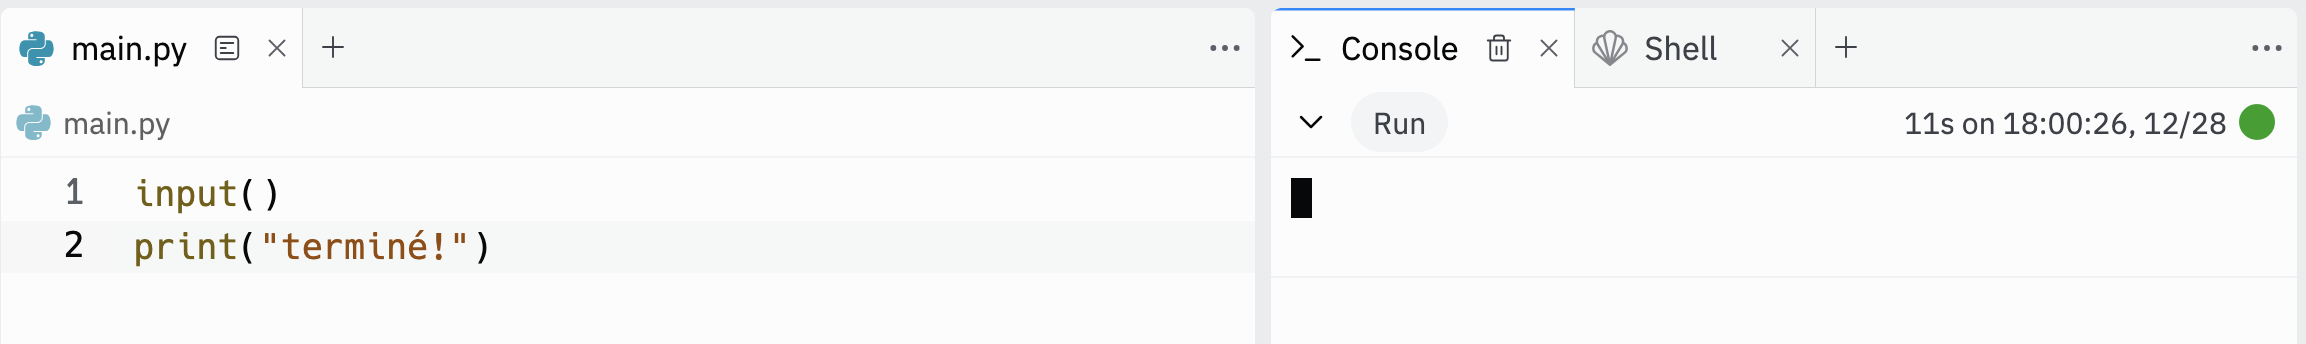
\includegraphics{./imgs/unidad_2/input1.png}

}

\caption{Input bloquea el flujo del programa}

\end{figure}%%
\begin{figure}[H]

{\centering 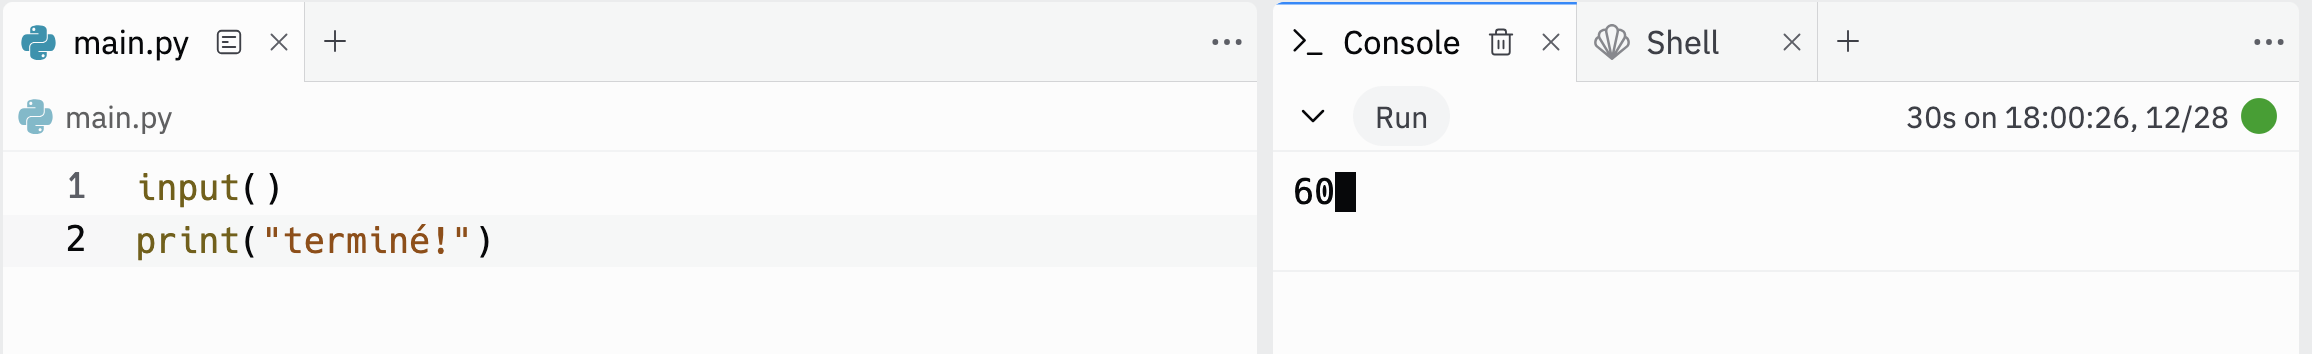
\includegraphics{./imgs/unidad_2/input2.png}

}

\caption{Ingresamos un valor (puede ser un número, texto, o ambos)}

\end{figure}%%
\begin{figure}[H]

{\centering 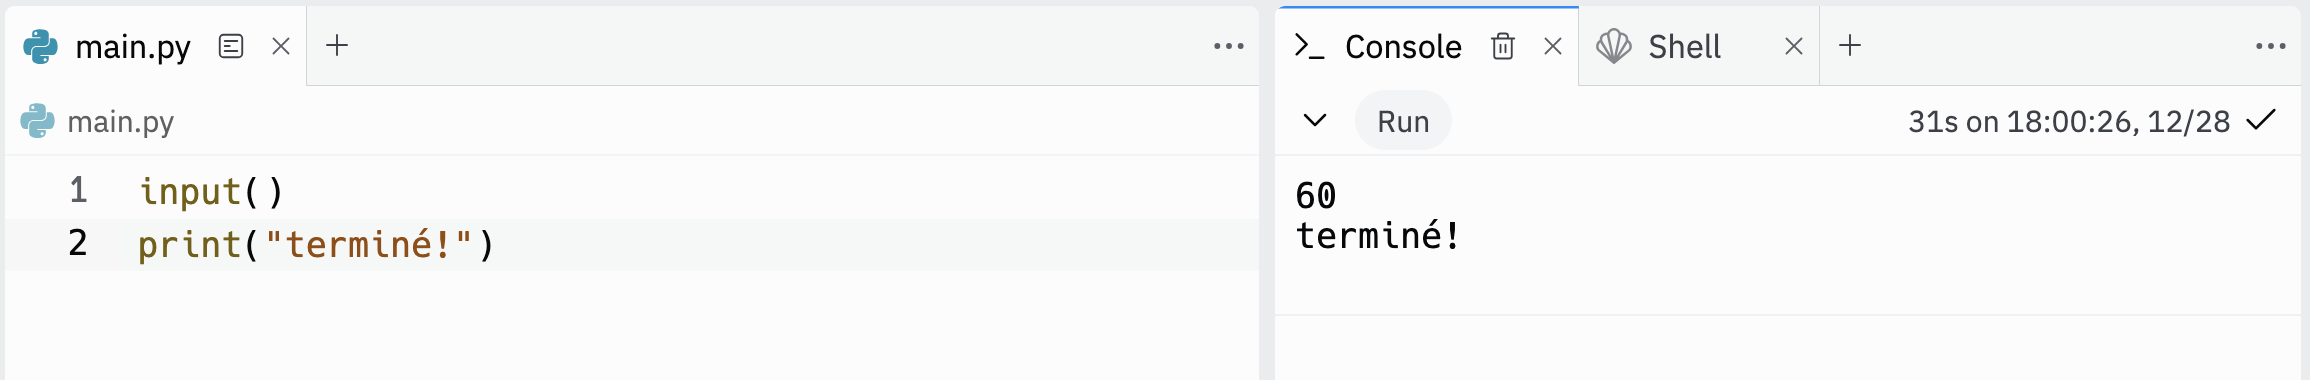
\includegraphics{./imgs/unidad_2/input3.png}

}

\caption{Al presionar Enter, la consola muestra el mensaje ``terminé!''}

\end{figure}%

\subsubsection{Obteniendo el Valor
Ingresado}\label{obteniendo-el-valor-ingresado}

Como dijimos más arriba, la función \texttt{input} devuelve el valor
ingresado por el usuario. Para poder usarlo, tenemos que guardarlo en
una variable.

\begin{Shaded}
\begin{Highlighting}[]
\NormalTok{nombre }\OperatorTok{=} \BuiltInTok{input}\NormalTok{()}
\BuiltInTok{print}\NormalTok{(}\StringTok{"Hola, "} \OperatorTok{+}\NormalTok{ nombre }\OperatorTok{+} \StringTok{"!"}\NormalTok{)}
\end{Highlighting}
\end{Shaded}

\begin{figure}[H]

{\centering 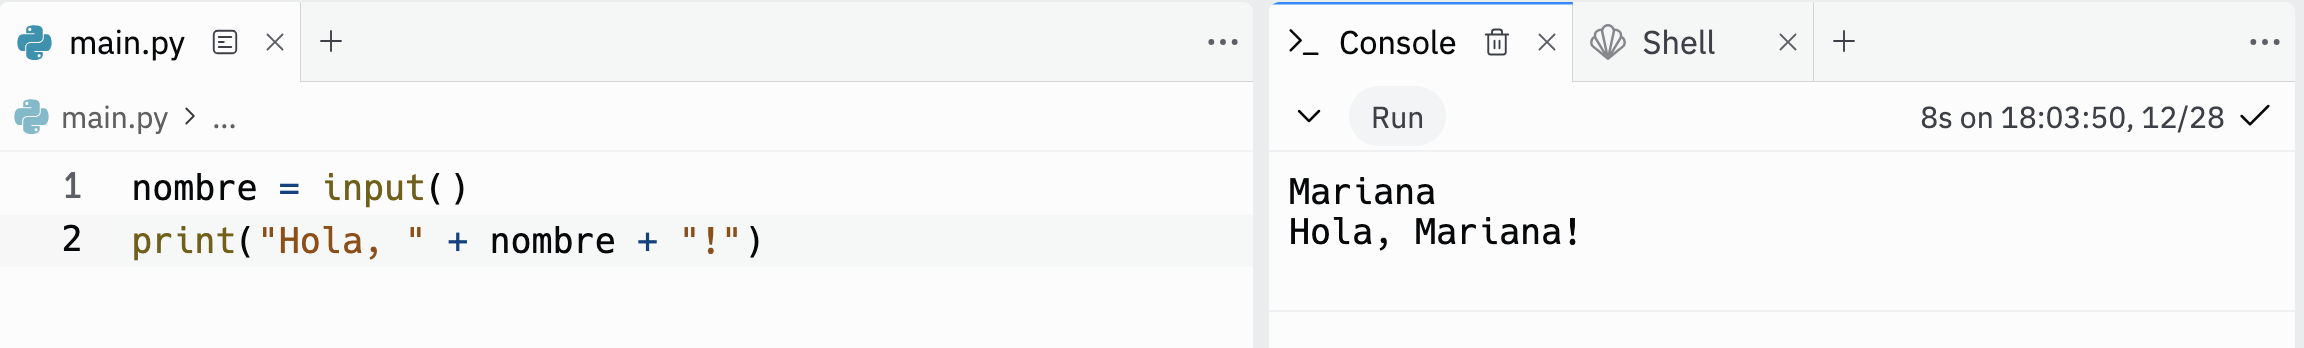
\includegraphics{./imgs/unidad_2/ejemplo_input1.png}

}

\caption{Ingresamos ``Mariana'' y presionamos Enter.}

\end{figure}%

Para hacer nuestro programa más amigable, podemos mostrarle al usuario
un mensaje antes de pedirle que ingrese un valor. Para esto, podemos
pasarle un parámetro a la función \texttt{input}, que es el mensaje que
queremos mostrarle al usuario.

\begin{Shaded}
\begin{Highlighting}[]
\NormalTok{nombre }\OperatorTok{=} \BuiltInTok{input}\NormalTok{(}\StringTok{"Ingresá tu nombre: "}\NormalTok{)}
\BuiltInTok{print}\NormalTok{(}\StringTok{"Hola, "} \OperatorTok{+}\NormalTok{ nombre }\OperatorTok{+} \StringTok{"!"}\NormalTok{)}
\end{Highlighting}
\end{Shaded}

\begin{figure}[H]

{\centering 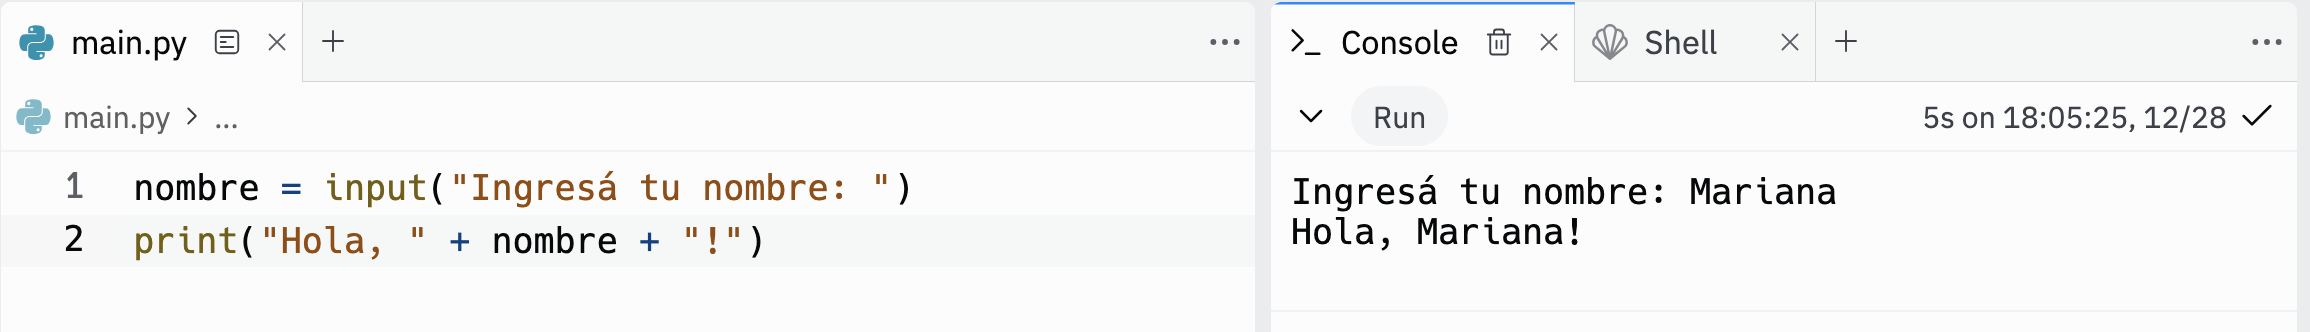
\includegraphics{./imgs/unidad_2/ejemplo_input2.png}

}

\caption{Ingresamos ``Mariana'' y presionamos Enter.}

\end{figure}%

\begin{tcolorbox}[enhanced jigsaw, bottomrule=.15mm, leftrule=.75mm, opacityback=0, colback=white, toprule=.15mm, bottomtitle=1mm, opacitybacktitle=0.6, rightrule=.15mm, left=2mm, arc=.35mm, coltitle=black, title=\textcolor{quarto-callout-warning-color}{\faExclamationTriangle}\hspace{0.5em}{¡Cuidado!}, breakable, toptitle=1mm, colframe=quarto-callout-warning-color-frame, titlerule=0mm, colbacktitle=quarto-callout-warning-color!10!white]

A partir de la guía 2, a menos que el ejercicio diga específicamente
``pedirle al usuario'', no se debe usar \texttt{input}, sino que todo
tiene que recibirse por parámetro en la función.

Lo mismo con \texttt{print}: A menos que el ejercicio diga
específicamente ``imprimir'', todo siempre se tiene que devolver con un
return.

\end{tcolorbox}

\section{Buenas Prácticas de
programación}\label{buenas-pruxe1cticas-de-programaciuxf3n}

\subsection{Sobre Comentarios}\label{sobre-comentarios}

Los comentarios son líneas que se escriben en el código, pero que no se
ejecutan. Sirven para que el programador pueda dejar notas en el código,
para que se entienda mejor qué hace el programa.\\
Los comentarios se escriben con el símbolo \texttt{\#}. Todo lo que esté
a la derecha del \texttt{\#} no se ejecuta. También se pueden encerrar
entre tres comillas dobles (\texttt{"""}) para escribir comentarios de
varias líneas.

\begin{Shaded}
\begin{Highlighting}[]
\CommentTok{\# Esto es un comentario}

\CommentTok{""" Esto es un comentario}
\CommentTok{de varias líneas """}
\end{Highlighting}
\end{Shaded}

No es correcto escribir comentarios que no aporten nada al código, o
tener el código absolutamente plagado de comentarios. Los comentarios
deben ser útiles, y deben aportar información que no se pueda inferir
del código. Nuestro primer intento de hacer el código más entendible no
tienen que ser los comentarios, sino mejorar el código en sí.

\subsection{Sobre Convención de
Nombres}\label{sobre-convenciuxf3n-de-nombres}

Para nombres de variables y funciones, se usa snake\_case, que es
básicamente dejar todas las palabras en minúscula y unirlas con un guión
bajo. Ejemplos: \texttt{numero\_positivo}, \texttt{sumar\_cinco},
\texttt{pedir\_numero}, etc.~ Siempre emplear un nombre que nos remita
al significado que tendrá ese dato, siempre en snake\_case:
\texttt{numero}, \texttt{letra}, \texttt{letra2},
\texttt{edad\_hermano}, etc.

\subsubsection{Variables}\label{variables-1}

Las variables son cosas. Entonces sus nombres son sustantivos:
\texttt{nombre}, \texttt{numero}, \texttt{suma}, \texttt{resta},
\texttt{resultado}, \texttt{respuesta\_usuario}. La única excepción son
las variables booleanas (ya las vamos a ver, son aquellas que pueden
guardar dos posibles valores: verdadero o falso), que suelen tener
nombres como \texttt{es\_par}, \texttt{es\_cero}, \texttt{es\_entero},
porque su valor es true o false.

A veces es útil alguna frase para identificar mejor el contenido:\\
\texttt{edad\_mayor\_hijo}, \texttt{apellido\_conyuge}

\subsubsection{Funciones}\label{funciones-1}

Las funciones hacen algo. Entonces sus nombres son verbos. Se usan
siempre verbos en infinitivo (terminan en \texttt{-ar}, \texttt{-er},
\texttt{-ir}): \texttt{calcular\_suma}, \texttt{imprimir\_mensaje},
\texttt{correr\_prueba}, \texttt{obtener\_triplicado}, etc.\\
De nuevo, las excepciones son las funciones que devuelven un valor
booleano (V o F). Esas pueden llamarse como: \texttt{es\_par},
\texttt{da\_cero}, \texttt{tiene\_letra\_a}, porque devuelven verdadero
o falso, y eso nos confirma o niega la afirmación que hace el nombre.

\subsection{Sobre Ordenamiento de
Código}\label{sobre-ordenamiento-de-cuxf3digo}

Cuando uno corre Python, lo que hace el lenguaje es leer línea a línea
nuestro código. Lo que se puede ejecutar, lo ejecuta. Las funciones las
guarda en memoria para poder usarlas luego.\\
Entonces es más ordenado y prolijo primero poner todas las funciones, y
después el código ``ejecutable'' (si van a dejar código suelto en el
archivo).\\

Además, no olvidemos que Python tiene un flujo de control de arriba para
abajo. Si intentamos invocar funciones antes de que estén definidas
(\texttt{def}), Python no va a saber qué hacer, y nos va a tirar un
error.\\

\textbf{Esto es correcto:}

\textbf{Esto es incorrecto:}

\subsection{Sobre uso de Parámetros en
Funciones}\label{sobre-uso-de-paruxe1metros-en-funciones}

Una función se puede pensar como una caja cerrada o una fábrica. La
función tiene dos puertas: una de entrada y una de salida.\\
La puerta de entrada son los \texttt{parámetros} y la de salida es el
\texttt{output} (el resultado).

Cuando se llama o invoca a la función, la puerta de entrada se abre,
permitiéndonos enviarle (pasarle) cero, uno o más parámetros a la
función (según cómo esté definida). Los parámetros son datos que la
función necesida para funcionar, y como ya dijimos, se le pasan a la
misma entre los paréntesis de la llamada.\\

\begin{quote}
\textbf{Ejemplo:} \texttt{saludar(nombre)},
\texttt{imprimir\_elementos(lista)}, \texttt{sumar(numero1,\ numero2)},
etc.
\end{quote}

Una vez que la función se empieza a ejecutar, ambas puertas se cierran.
Esto quiere decir que, mientras la función se está ejecutando, nada
entra y nada sale de la misma.\\
La función debería trabajar únicamente con los datos que se le hayan
pasado por parámetro o que se le pidan al usuario dentro de ella, pero
no debería utilizar nada que esté por fuera de la misma.

\begin{tcolorbox}[enhanced jigsaw, bottomrule=.15mm, leftrule=.75mm, opacityback=0, colback=white, toprule=.15mm, bottomtitle=1mm, opacitybacktitle=0.6, rightrule=.15mm, left=2mm, arc=.35mm, coltitle=black, title=\textcolor{quarto-callout-warning-color}{\faExclamationTriangle}\hspace{0.5em}{¡Cuidado!}, breakable, toptitle=1mm, colframe=quarto-callout-warning-color-frame, titlerule=0mm, colbacktitle=quarto-callout-warning-color!10!white]

Python nos deja usar cosas por fuera de la función y sin recibir los
datos por parámetro, porque es un lenguaje muy benevolente. Pero está
mal usar cosas que no se hayan recibido por parámetro: es una mala
práctica.

\end{tcolorbox}

Una vez que la función terminó de ejecutarse, el o los valores de salida
(resultados) se devuelven por el output. Una función puede retornar uno
o más elementos, o podría simplemente no retornar nada.\\
\texttt{return\ suma}, \texttt{return\ numero1,\ numero2},
\texttt{return}, etc.

Podemos ver la diferencia entre enviar algo por parámetro y usarlo por
fuera de la función a continuación:

Esto está mal

Esto está bien

\begin{Shaded}
\begin{Highlighting}[]
\KeywordTok{def}\NormalTok{ saludar():}
  \BuiltInTok{print}\NormalTok{(}\StringTok{"Hola, "} \OperatorTok{+}\NormalTok{ nombre }\OperatorTok{+} \StringTok{"!"}\NormalTok{)}

\NormalTok{nombre }\OperatorTok{=} \StringTok{"Manuela"}
\NormalTok{saludar()}
\end{Highlighting}
\end{Shaded}

\begin{Shaded}
\begin{Highlighting}[]
\KeywordTok{def}\NormalTok{ saludar(persona):}
  \BuiltInTok{print}\NormalTok{(}\StringTok{"Hola, "} \OperatorTok{+}\NormalTok{ persona }\OperatorTok{+} \StringTok{"!"}\NormalTok{)}

\NormalTok{nombre }\OperatorTok{=} \StringTok{"Manuela"}
\NormalTok{saludar(nombre)}
\end{Highlighting}
\end{Shaded}

\begin{tcolorbox}[enhanced jigsaw, bottomrule=.15mm, leftrule=.75mm, opacityback=0, colback=white, toprule=.15mm, bottomtitle=1mm, opacitybacktitle=0.6, rightrule=.15mm, left=2mm, arc=.35mm, coltitle=black, title=\textcolor{quarto-callout-tip-color}{\faLightbulb}\hspace{0.5em}{Tip}, breakable, toptitle=1mm, colframe=quarto-callout-tip-color-frame, titlerule=0mm, colbacktitle=quarto-callout-tip-color!10!white]

Como podemos observar los nombres de los argumentos cuando se invoca y
en la definición de la firma pueden ser los mismos o distintos. En este
caso, la función sabe que está recibiendo algo como parámetro, y sabe
que dentro de su cuerpo a este dato lo va a identificar como
\texttt{persona}, pero no hace falta que la variable que nosotros le
pasamos como parámetro también se llame \texttt{persona}: en este caso
se llama \texttt{nombre}.\\

\end{tcolorbox}

\section{Tipos de Datos}\label{tipos-de-datos}

\subsection{Datos Simples}\label{datos-simples}

Los programas trabajan con una gran variedad de datos. Los datos más
simples son los que ya vimos: números enteros, números de punto flotante
y cadenas.\\
Pero dependiendo de la naturaleza o el \textbf{tipo} de información,
cabrá la posibilidad de realizar distintas transformaciones aplicando
\textbf{operadores}. Por eso, a la hora de representar información no
sólo es importante que identifiquemos al dato y podamos conocer su
valor, sino saber qué tipo de tratamiento podemos darle.

Todos los lenguajes tienen tipos predefinidos de datos. Se llaman
predefinidos porque el lenguaje ya los conoce: sabe cómo guardarlos en
memoria y qué transformaciones puede aplicarles.

En Python, tenemos los siguientes tipos de datos:

\begin{longtable}[]{@{}
  >{\centering\arraybackslash}p{(\columnwidth - 4\tabcolsep) * \real{0.3333}}
  >{\centering\arraybackslash}p{(\columnwidth - 4\tabcolsep) * \real{0.3333}}
  >{\centering\arraybackslash}p{(\columnwidth - 4\tabcolsep) * \real{0.3333}}@{}}
\toprule\noalign{}
\begin{minipage}[b]{\linewidth}\centering
Tipo
\end{minipage} & \begin{minipage}[b]{\linewidth}\centering
Descripción
\end{minipage} & \begin{minipage}[b]{\linewidth}\centering
Ejemplo
\end{minipage} \\
\midrule\noalign{}
\endhead
\bottomrule\noalign{}
\endlastfoot
\texttt{int} & Números enteros & \texttt{5}, \texttt{0}, \texttt{-5},
\texttt{10000} \\
\texttt{float} & Números de punto flotante o reales & \texttt{3.14159},
\texttt{1.0}, \texttt{0.0} \\
\texttt{complex} & Números complejos & \texttt{(1,\ 2j)},
\texttt{(1.0,-2.0j)}, \texttt{(0,1j)}. La componente con \texttt{j} es
la parte imaginaria. \\
\texttt{bool} & Valores booleanos o valores lógicos & \texttt{True},
\texttt{False} \\
\texttt{str} & Cadenas de caracteres & \texttt{"Hola"},
\texttt{"Python"}, \texttt{"¡Hola,\ mundo!"}, \texttt{""} (cadena vacía,
no contiene ningún caracter) \\
\end{longtable}

\begin{tcolorbox}[enhanced jigsaw, bottomrule=.15mm, leftrule=.75mm, opacityback=0, colback=white, toprule=.15mm, bottomtitle=1mm, opacitybacktitle=0.6, rightrule=.15mm, left=2mm, arc=.35mm, coltitle=black, title=\textcolor{quarto-callout-note-color}{\faInfo}\hspace{0.5em}{¿Por qué se llaman ``cadenas de caracteres''?}, breakable, toptitle=1mm, colframe=quarto-callout-note-color-frame, titlerule=0mm, colbacktitle=quarto-callout-note-color!10!white]

Porque son una cadena de caracteres, es decir, una secuencia de
caracteres. Por ejemplo, la cadena ``Hola'' está formada por los
caracteres ``H'', ``o'', ``l'' y ``a''.~Esto nos permite acceder a cada
uno de los caracteres de la cadena por separado si quisiéramos, o a
porciones de una cadena, como vamos a ver más adelante.\\
Más aún, podemos ver que el texto ``hola'' no será igual a ``aloh'' ni a
``Holá'', porque son cadenas distintas.\\
Un string permite almacenar cualquier tipo de caracter unicode dentro
(letras, números, símbolos, emojis, etc.).

\end{tcolorbox}

\subsection{Operadores Numéricos}\label{operadores-numuxe9ricos}

Los operadores son símbolos que representan una operación. Por ejemplo,
el operador \texttt{+} representa la suma.\\

Para transformar datos numéricos, emplearemos los siguientes operadores:

\begin{longtable}[]{@{}ccc@{}}
\toprule\noalign{}
Símbolo & Definición & Ejemplo \\
\midrule\noalign{}
\endhead
\bottomrule\noalign{}
\endlastfoot
\texttt{+} & Suma & \texttt{5\ +\ 3} \\
\texttt{-} & Resta & \texttt{5\ -\ 3} \\
\texttt{*} & Producto & \texttt{5\ *\ 3} \\
\texttt{**} & Potencia & \texttt{5\ **\ 2} \\
\texttt{/} & División & \texttt{5\ /\ 3} \\
\texttt{//} & División entera & \texttt{5\ //\ 3} \\
\texttt{\%} & Módulo o Resto & \texttt{5\ \%\ 3} \\
\texttt{+=} & Suma abreviada & \texttt{x\ =\ 0}\texttt{x\ +=\ 3} \\
\texttt{-=} & Resta abreviada & \texttt{x\ =\ 0}\texttt{x\ -=\ 3} \\
\texttt{*=} & Producto abreviado & \texttt{x\ =\ 0}\texttt{x\ *=\ 3} \\
\texttt{/=} & División abreviada & \texttt{x\ =\ 0}\texttt{x\ /=\ 3} \\
\texttt{//=} & División entera abreviada &
\texttt{x\ =\ 0}\texttt{x\ //=\ 3} \\
\texttt{\%=} & Módulo o Resto abreviado &
\texttt{x\ =\ 0}\texttt{x\ \%=\ 3} \\
\end{longtable}

Como pasa en matemática, para alterar cualquier precedencia (prioridad
de operadores) se pueden usar paréntesis.

\begin{Shaded}
\begin{Highlighting}[]
\NormalTok{(}\DecValTok{5} \OperatorTok{+} \DecValTok{3}\NormalTok{) }\OperatorTok{*} \DecValTok{2}
\end{Highlighting}
\end{Shaded}

\begin{verbatim}
16
\end{verbatim}

\begin{Shaded}
\begin{Highlighting}[]
\DecValTok{5} \OperatorTok{+}\NormalTok{ (}\DecValTok{3} \OperatorTok{*} \DecValTok{2}\NormalTok{)}
\end{Highlighting}
\end{Shaded}

\begin{verbatim}
11
\end{verbatim}

El orden de prioridad de ejecución para los operadores va a ser el mismo
que en matemática.

\subsection{Operadores de Texto}\label{operadores-de-texto}

Para transformar datos de texto, emplearemos los siguientes operadores:

\begin{longtable}[]{@{}
  >{\centering\arraybackslash}p{(\columnwidth - 4\tabcolsep) * \real{0.3333}}
  >{\centering\arraybackslash}p{(\columnwidth - 4\tabcolsep) * \real{0.3333}}
  >{\centering\arraybackslash}p{(\columnwidth - 4\tabcolsep) * \real{0.3333}}@{}}
\toprule\noalign{}
\begin{minipage}[b]{\linewidth}\centering
Símbolo
\end{minipage} & \begin{minipage}[b]{\linewidth}\centering
Definición
\end{minipage} & \begin{minipage}[b]{\linewidth}\centering
Ejemplo
\end{minipage} \\
\midrule\noalign{}
\endhead
\bottomrule\noalign{}
\endlastfoot
\texttt{+} & Concatenación & \texttt{"Hola"\ +\ "\ "\ +\ "Mundo"} \\
\texttt{*} & Repetición & \texttt{"Hola"\ *\ 3} \\
\texttt{+=} & Concatenación abreviada &
\texttt{x\ =\ "Hola"}\texttt{x\ +=\ "\ Mundo"} \\
\texttt{*=} & Repetición abreviada &
\texttt{x\ =\ "Hola"}\texttt{x\ *=\ 3} \\
{[}k{]} o {[}-k{]} & Acceso a un caracter &
\texttt{"Hola"{[}0{]}}\texttt{"Hola"{[}-1{]}} \\
{[}k1:k2{]} & Acceso a una porción &
\texttt{"Hola"{[}0:2{]}}\texttt{"Hola"{[}1:{]}}\texttt{"Hola"{[}:2{]}}\texttt{"Hola"{[}:{]}} \\
\end{longtable}

De nuevo, para alterar precedencias, se deben usar \texttt{()}.

\subsubsection{Manipulando Strings}\label{manipulando-strings}

Si bien esto se va a ahondar en la siguiente sesión de la materia, es
importante saber que los strings, como se dijo más arriba, son un
conjunto de caracteres. Pero no sólo un conjunto, sino un
\textbf{conjunto ordenado}. Esto quiere decir que cada caracter tiene
una posición dentro de la cadena, y que esa posición es importante.\\

Por ejemplo, la cadena \texttt{"Hola"} tiene 4 caracteres: \texttt{"H"},
\texttt{"o"}, \texttt{"l"} y \texttt{"a"}.\\
La posición de cada caracter es la siguiente:

\begin{longtable}[]{@{}ccccc@{}}
\toprule\noalign{}
Posición & 0 & 1 & 2 & 3 \\
\midrule\noalign{}
\endhead
\bottomrule\noalign{}
\endlastfoot
Caracter & ``H'' & ``o'' & ``l'' & ``a'' \\
\end{longtable}

Entonces, si queremos acceder al caracter \texttt{"H"}, tenemos que usar
la posición 0. Si queremos acceder al caracter \texttt{"a"}, tenemos que
usar la posición 3.\\

\begin{tcolorbox}[enhanced jigsaw, bottomrule=.15mm, leftrule=.75mm, opacityback=0, colback=white, toprule=.15mm, bottomtitle=1mm, opacitybacktitle=0.6, rightrule=.15mm, left=2mm, arc=.35mm, coltitle=black, title=\textcolor{quarto-callout-tip-color}{\faLightbulb}\hspace{0.5em}{Tip}, breakable, toptitle=1mm, colframe=quarto-callout-tip-color-frame, titlerule=0mm, colbacktitle=quarto-callout-tip-color!10!white]

Para acceder a un caracter de una cadena, usamos los corchetes
(\texttt{{[}{]}}) y dentro de ellos la posición del caracter que
queremos acceder.\\

\end{tcolorbox}

\begin{Shaded}
\begin{Highlighting}[]
\NormalTok{letra }\OperatorTok{=} \StringTok{"Hola"}\NormalTok{[}\DecValTok{0}\NormalTok{]}
\BuiltInTok{print}\NormalTok{(letra)}
\end{Highlighting}
\end{Shaded}

\begin{verbatim}
H
\end{verbatim}

Pero no sólo puedo obtener los caracteres en las posicione de la
palabra, sino que puedo obtener \emph{slices} o \emph{porciones} de la
misma, usando algo que vemos por primera vez: los \textbf{rangos}.

Un rango tiene tres partes:

\begin{Shaded}
\begin{Highlighting}[]
\NormalTok{[start : end : step]}
\end{Highlighting}
\end{Shaded}

\begin{itemize}
\tightlist
\item
  \texttt{start} es el índice de inicio del rango. Si no se especifica,
  se toma el índice 0. El caracter en la posición de inicio siempre se
  incluye.
\item
  \texttt{end} es el índice de fin del rango. Si no se especifica, se
  toma el índice final de la cadena. El caracter en la posición de fin
  nunca se incluye.
\item
  \texttt{step} es el tamaño del paso. Si no se especifica, se toma el
  valor 1.
\end{itemize}

\begin{quote}
\textbf{Ejemplos:}
\end{quote}

\subsection{Input y Casteo}\label{input-y-casteo}

Cuando usamos la función \texttt{input}, el valor que devuelve es
siempre una cadena. Esto es porque el usuario puede ingresar cualquier
cosa, y no sabemos qué tipo de dato es.\\

Por ejemplo, si le pedimos al usuario que ingrese un número, el usuario
puede ingresar un número entero, un número de punto flotante, un número
complejo, o incluso un texto. Entonces, el valor que devuelve
\texttt{input} es siempre una cadena, y nosotros tenemos que
transformarla al tipo de dato que necesitemos.\\

Por ejemplo:

\begin{Shaded}
\begin{Highlighting}[]
\NormalTok{edad }\OperatorTok{=} \BuiltInTok{input}\NormalTok{(}\StringTok{"Indique su edad:"}\NormalTok{)}
\BuiltInTok{print}\NormalTok{(}\StringTok{"Su edad es:"}\NormalTok{, edad\_nueva)}
\end{Highlighting}
\end{Shaded}

\begin{tcolorbox}[enhanced jigsaw, bottomrule=.15mm, leftrule=.75mm, opacityback=0, colback=white, toprule=.15mm, bottomtitle=1mm, opacitybacktitle=0.6, rightrule=.15mm, left=2mm, arc=.35mm, coltitle=black, title=\textcolor{quarto-callout-tip-color}{\faLightbulb}\hspace{0.5em}{Imprimiendo Strings y Variables (Iterpolación de Cadenas)}, breakable, toptitle=1mm, colframe=quarto-callout-tip-color-frame, titlerule=0mm, colbacktitle=quarto-callout-tip-color!10!white]

Existen muchas formas de concatenar variables con texto.

\begin{enumerate}
\def\labelenumi{\arabic{enumi}.}
\tightlist
\item
  Usando el operador \texttt{+}: \texttt{"Su\ edad\ es:\ "\ +\ edad}
\item
  Usando el método \texttt{fstring}: \texttt{f"Su\ edad\ es:\ \{edad\}"}
\item
  Usando el caracter \texttt{,}: \texttt{print("Su\ edad\ es:",\ edad)}
\end{enumerate}

La forma más recomendada es la segunda, usando \texttt{fstring}. Pero
dependerá de cada caso.

\end{tcolorbox}

El problema es que, si bien nuestro código anterior funciona, no podemos
operar \texttt{edad} como si fuese un número, porque es un string.\\
El siguiente código va a fallar:

\begin{Shaded}
\begin{Highlighting}[]
\NormalTok{edad }\OperatorTok{=} \BuiltInTok{input}\NormalTok{(}\StringTok{"Indique su edad:"}\NormalTok{)}
\NormalTok{edad\_nueva }\OperatorTok{=}\NormalTok{ edad }\OperatorTok{+} \DecValTok{1}
\BuiltInTok{print}\NormalTok{(}\StringTok{"Edad siguiente:"}\NormalTok{, edad\_nueva)}
\end{Highlighting}
\end{Shaded}

\begin{figure}[H]

{\centering 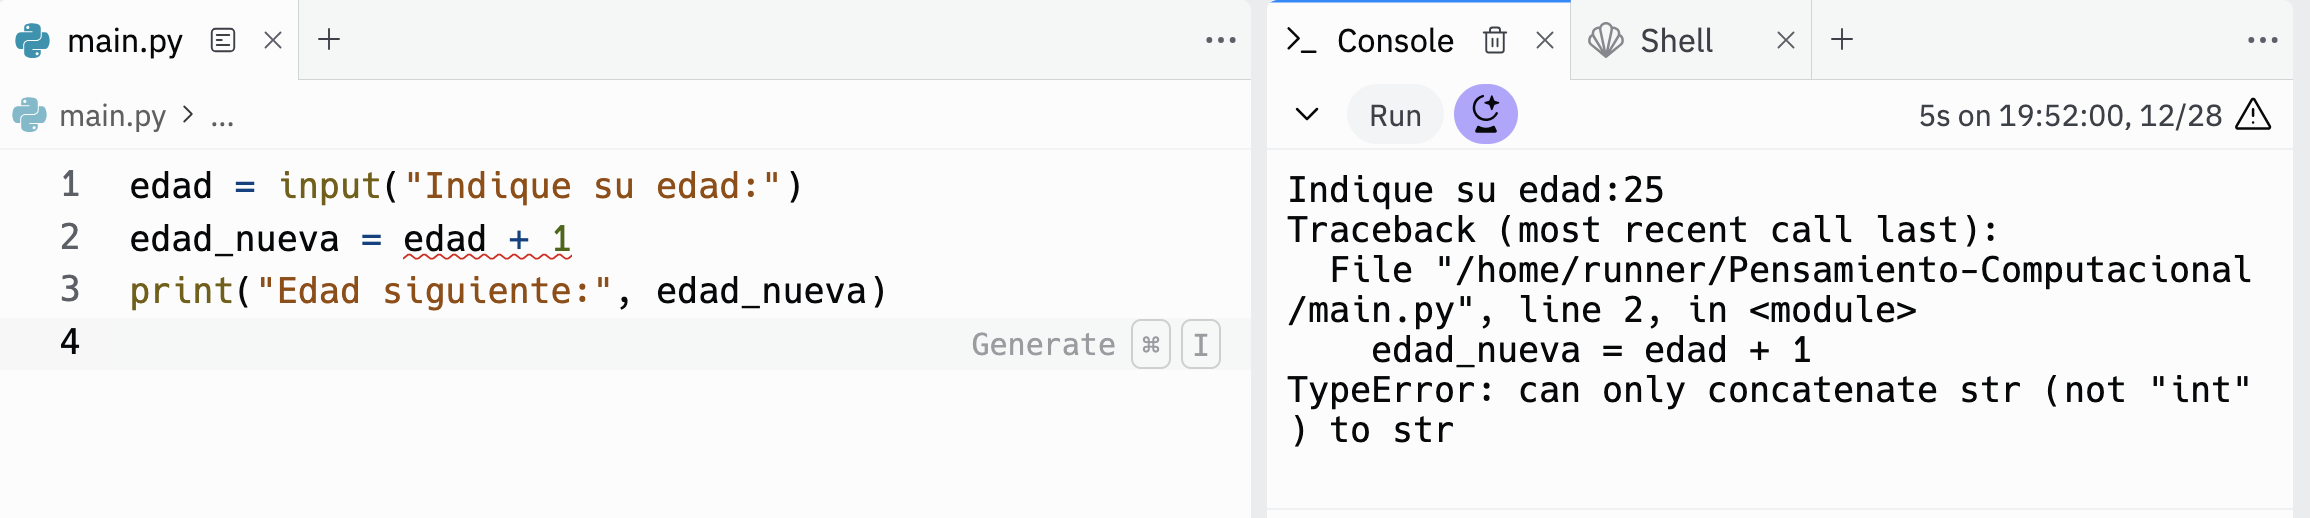
\includegraphics{./imgs/unidad_2/error_input1.png}

}

\caption{Ejecución del bloque de código}

\end{figure}%

Como vemos, la consola nos arroja un error, o en términos simples
decimos que ``explotó''.

\begin{tcolorbox}[enhanced jigsaw, bottomrule=.15mm, leftrule=.75mm, opacityback=0, colback=white, toprule=.15mm, bottomtitle=1mm, opacitybacktitle=0.6, rightrule=.15mm, left=2mm, arc=.35mm, coltitle=black, title=\textcolor{quarto-callout-tip-color}{\faLightbulb}\hspace{0.5em}{¿Qué es un error?}, breakable, toptitle=1mm, colframe=quarto-callout-tip-color-frame, titlerule=0mm, colbacktitle=quarto-callout-tip-color!10!white]

Los errores son información que nos da la consola para que podamos
corregir nuestro código.

\end{tcolorbox}

En este caso, nos dice que no se puede concatenar un string con un
int.\\
¿Por qué nos dice eso? Porque \texttt{edad} es un string: \texttt{"25"},
y estamos tratando de sumarle 1, que es un int: \texttt{1}.\\

Para poder operar con \texttt{edad} como si fuese un número, tenemos que
transformarla a un número. Esto se llama \textbf{castear}.\\

Para castear un valor a un tipo de dato, usamos el nombre del tipo de
dato, seguido de paréntesis y el valor que queremos castear.

\begin{Shaded}
\begin{Highlighting}[]
\BuiltInTok{int}\NormalTok{(}\StringTok{"25"}\NormalTok{)}
\end{Highlighting}
\end{Shaded}

De esta forma, podemos modificar nuestro código anterior:

\begin{Shaded}
\begin{Highlighting}[]
\NormalTok{edad }\OperatorTok{=} \BuiltInTok{int}\NormalTok{(}\BuiltInTok{input}\NormalTok{(}\StringTok{"Indique su edad:"}\NormalTok{)) }\CommentTok{\# Le agregamos int}
\NormalTok{edad\_nueva }\OperatorTok{=}\NormalTok{ edad }\OperatorTok{+} \DecValTok{1}
\BuiltInTok{print}\NormalTok{(}\StringTok{"Edad siguiente:"}\NormalTok{, edad\_nueva)}
\end{Highlighting}
\end{Shaded}

Y obtenemos un código que funciona correctamente.

\begin{figure}[H]

{\centering 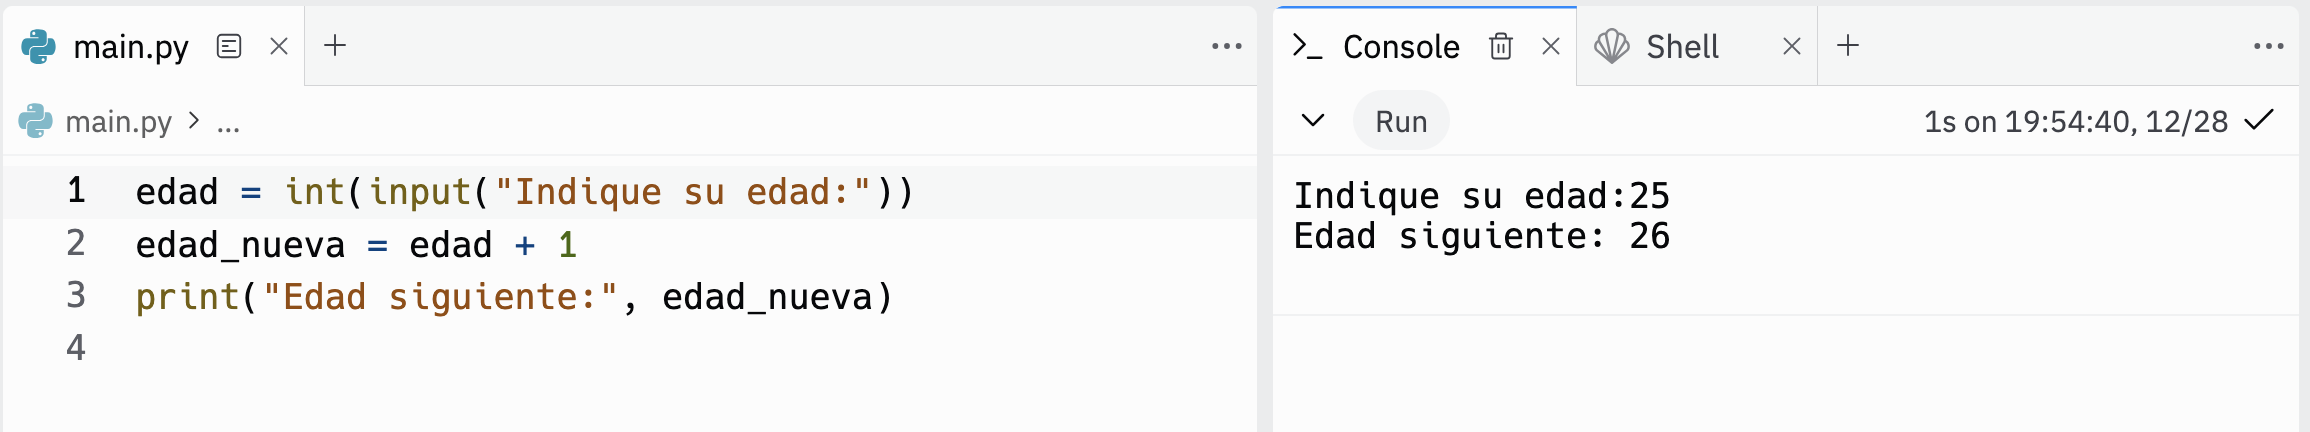
\includegraphics{./imgs/unidad_2/error_input2.png}

}

\caption{Ejecución del bloque de código}

\end{figure}%

De esta forma, podemos castear a varios tipos de datos:

\begin{Shaded}
\begin{Highlighting}[]
\NormalTok{numero\_entero }\OperatorTok{=} \BuiltInTok{int}\NormalTok{(}\BuiltInTok{input}\NormalTok{(}\StringTok{"Ingrese un número"}\NormalTok{))}
\NormalTok{punto\_flotante }\OperatorTok{=} \BuiltInTok{float}\NormalTok{(}\BuiltInTok{input}\NormalTok{(}\StringTok{"Ingrese un número"}\NormalTok{))}

\NormalTok{punto\_flotante2 }\OperatorTok{=} \BuiltInTok{float}\NormalTok{(numero\_entero)}

\NormalTok{numero\_en\_str }\OperatorTok{=} \BuiltInTok{str}\NormalTok{(numero\_entero)}
\end{Highlighting}
\end{Shaded}

Ejemplo:

\begin{Shaded}
\begin{Highlighting}[]
\NormalTok{nombre\_menor }\OperatorTok{=} \BuiltInTok{input}\NormalTok{(}\StringTok{\textquotesingle{}Ingresá el nombre de un conocido/a:\textquotesingle{}}\NormalTok{)}
\NormalTok{edad\_menor }\OperatorTok{=} \BuiltInTok{int}\NormalTok{(}\BuiltInTok{input}\NormalTok{(}\SpecialStringTok{f\textquotesingle{}Ingresá la edad de }\SpecialCharTok{\{}\NormalTok{ nombre\_menor }\SpecialCharTok{\}}\SpecialStringTok{ \textquotesingle{}}\NormalTok{))}
\NormalTok{nombre\_mayor }\OperatorTok{=} \BuiltInTok{input}\NormalTok{(}\SpecialStringTok{f\textquotesingle{}Cómo se llama el hermano/a mayor de }\SpecialCharTok{\{}\NormalTok{nombre\_menor}\SpecialCharTok{\}}\SpecialStringTok{? \textquotesingle{}}\NormalTok{)}
\NormalTok{diferencia }\OperatorTok{=} \BuiltInTok{int}\NormalTok{(}\BuiltInTok{input}\NormalTok{(}\SpecialStringTok{f\textquotesingle{}Cuántos años más grande es }\SpecialCharTok{\{}\NormalTok{nombre\_mayor}\SpecialCharTok{\}}\SpecialStringTok{?  \textquotesingle{}}\NormalTok{))}

\NormalTok{edad\_mayor }\OperatorTok{=}\NormalTok{ edad\_menor }\OperatorTok{+}\NormalTok{ diferencia}

\BuiltInTok{print}\NormalTok{(nombre\_menor,}\StringTok{\textquotesingle{}tiene\textquotesingle{}}\NormalTok{,edad\_menor,}\StringTok{\textquotesingle{}años\textquotesingle{}}\NormalTok{)}
\BuiltInTok{print}\NormalTok{(nombre\_mayor,}\StringTok{\textquotesingle{}es mayor y tiene\textquotesingle{}}\NormalTok{, edad\_mayor, }\StringTok{\textquotesingle{}años\textquotesingle{}}\NormalTok{)}
\end{Highlighting}
\end{Shaded}

\begin{figure}[H]

{\centering 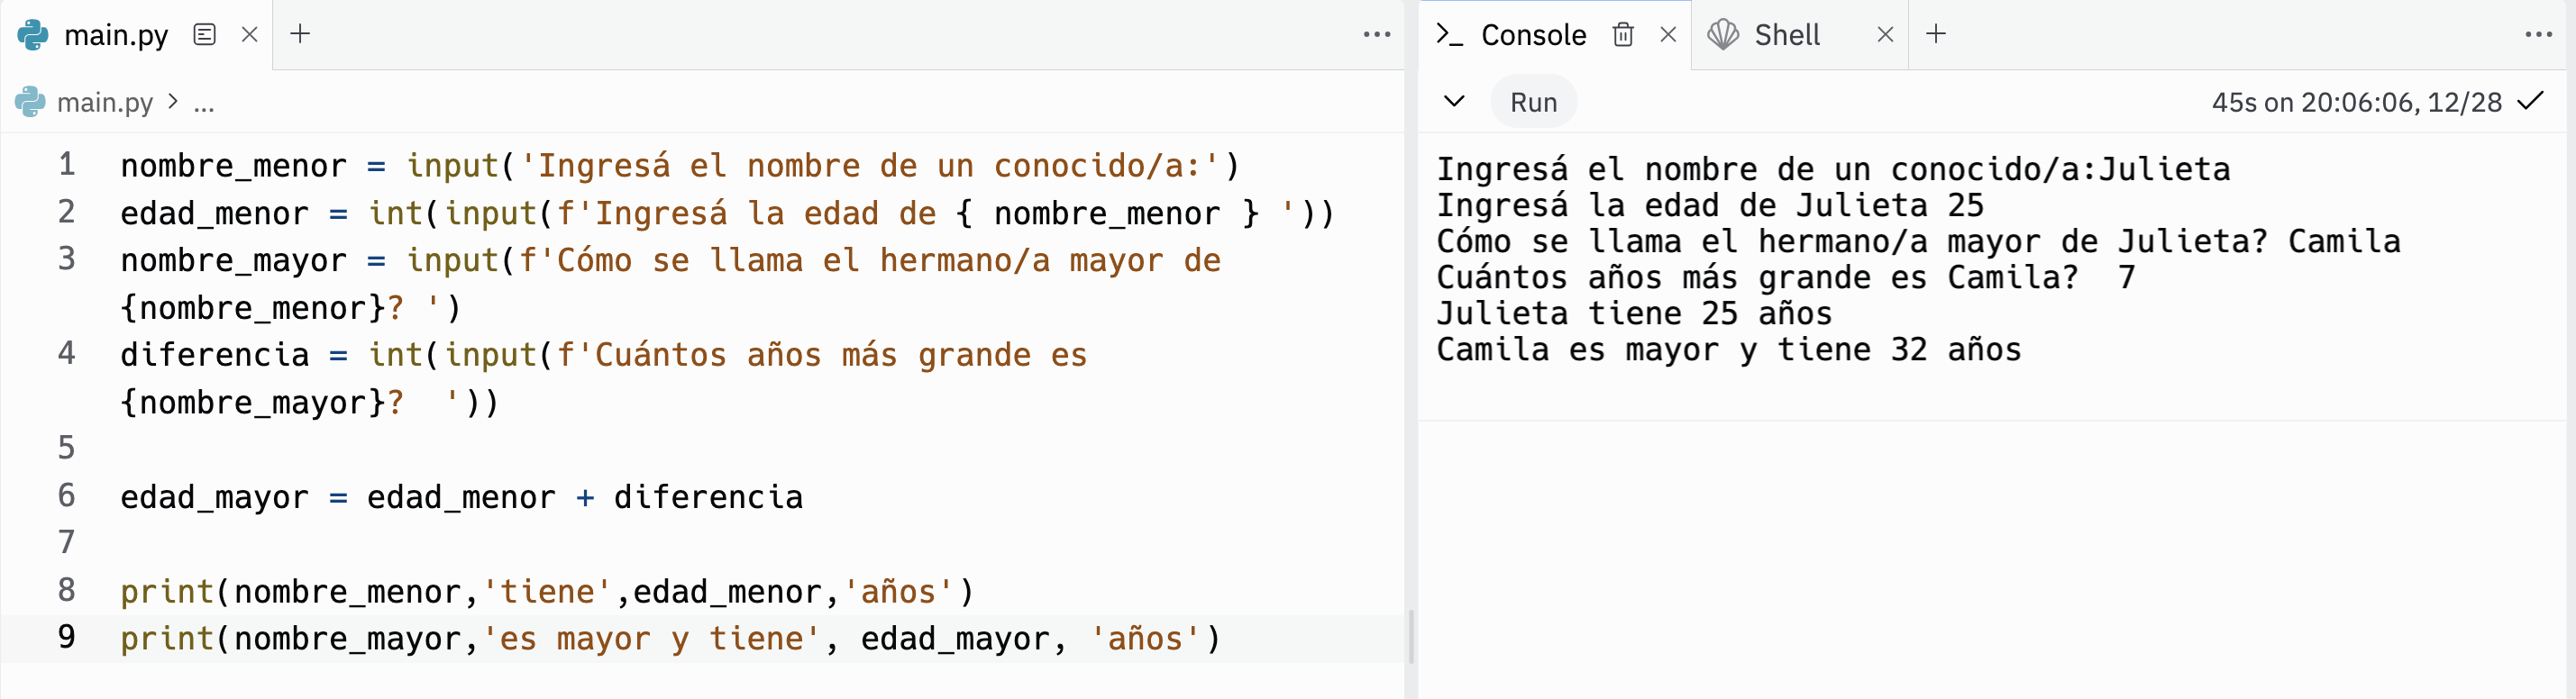
\includegraphics{./imgs/unidad_2/ejemplo_casteo.png}

}

\caption{Ejecución del bloque de código}

\end{figure}%

\section{Bonus Track: Algunas Funciones Predefinidas de
Python}\label{bonus-track-algunas-funciones-predefinidas-de-python}

\begin{tcolorbox}[enhanced jigsaw, bottomrule=.15mm, leftrule=.75mm, opacityback=0, colback=white, toprule=.15mm, bottomtitle=1mm, opacitybacktitle=0.6, rightrule=.15mm, left=2mm, arc=.35mm, coltitle=black, title=\textcolor{quarto-callout-note-color}{\faInfo}\hspace{0.5em}{Recomendación}, breakable, toptitle=1mm, colframe=quarto-callout-note-color-frame, titlerule=0mm, colbacktitle=quarto-callout-note-color!10!white]

Te recomendamos que te animes a probar estas funciones, para ver qué
hacen y terminar de entenderlas.

\end{tcolorbox}

\begin{longtable}[]{@{}
  >{\centering\arraybackslash}p{(\columnwidth - 4\tabcolsep) * \real{0.3333}}
  >{\centering\arraybackslash}p{(\columnwidth - 4\tabcolsep) * \real{0.3333}}
  >{\centering\arraybackslash}p{(\columnwidth - 4\tabcolsep) * \real{0.3333}}@{}}
\toprule\noalign{}
\begin{minipage}[b]{\linewidth}\centering
Función
\end{minipage} & \begin{minipage}[b]{\linewidth}\centering
Definición
\end{minipage} & \begin{minipage}[b]{\linewidth}\centering
Ejemplo de uso
\end{minipage} \\
\midrule\noalign{}
\endhead
\bottomrule\noalign{}
\endlastfoot
\texttt{print()} & Imprime un mensaje o valor en la consola &
\texttt{print("Hello,\ world!")} \\
\texttt{input()} & Lee una entrada de texto desde el usuario &
\texttt{name\ =\ input("Enter\ your\ name:\ ")} \\
\texttt{abs()} & Devuelve el valor absoluto de un número &
\texttt{abs(-5)} \\
\texttt{round()} & Redondea un número al entero más cercano &
\texttt{round(3.7)} \\
\texttt{int()} & Convierte un valor en un entero &
\texttt{x\ =\ int("5")} \\
\texttt{float()} & Convierte un valor en un número de punto flotante &
\texttt{y\ =\ float("3.14")} \\
\texttt{str()} & Convierte un valor en una cadena de texto &
\texttt{message\ =\ str(42)} \\
\texttt{bool()} & Convierte un valor en un booleano &
\texttt{is\_valid\ =\ bool(1)} \\
\texttt{len()} & Devuelve la longitud (número de elementos) de un objeto
& \texttt{length\ =\ len("Hello")} \\
\texttt{max()} & Devuelve el valor máximo entre varios elementos o una
secuencia & \texttt{max(4,\ 9,\ 2)} \\
\texttt{min()} & Devuelve el valor mínimo entre varios elementos o una
secuencia & \texttt{min(4,\ 9,\ 2)} \\
\texttt{pow()} & Calcula la potencia de un número &
\texttt{result\ =\ pow(2,\ 3)} \\
\texttt{range()} & Genera una secuencia de números &
\texttt{numbers\ =\ range(1,\ 5)} \\
\texttt{type()} & Devuelve el tipo de un objeto &
\texttt{data\_type\ =\ type("Hello")} \\
\texttt{round()} & Redondea un número a un número de decimales
específico & \texttt{rounded\_num\ =\ round(3.14159,\ 2)} \\
\texttt{isinstance()} & Verifica si un objeto es una instancia de una
clase específica & \texttt{is\_instance\ =\ isinstance(5,\ int)} \\
\texttt{replace()} & Reemplaza todas las apariciones de un substring por
otro &
\texttt{text\ =\ "Hello,\ World!"}\texttt{new\_text\ =\ text.replace("Hello",\ "Hi")} \\
\texttt{eval(\textless{}expr\textgreater{})} & Evalúa una expresión &
\texttt{eval("2\ +\ 2")} \\
\end{longtable}

\bookmarksetup{startatroot}

\chapter{Estructuras de Control}\label{estructuras-de-control}

\section{Decisiones}\label{decisiones}

\begin{quote}
\textbf{Ejemplo} Leer un número y, si el número es positivo, imprimir en
pantalla ``Número positivo''.
\end{quote}

Necesitamos \emph{decidir} de alguna forma si nuestro número \(x\) es
positivo (\textgreater0) o no. Para resolver este problema, introducimos
una nueva instrucción, llamada \emph{condicional}: \texttt{if}.

\begin{Shaded}
\begin{Highlighting}[]
\ControlFlowTok{if} \OperatorTok{\textless{}}\NormalTok{expresion}\OperatorTok{\textgreater{}}\NormalTok{:}
    \OperatorTok{\textless{}}\NormalTok{cuerpo}\OperatorTok{\textgreater{}}
\end{Highlighting}
\end{Shaded}

Donde \texttt{if} es una palabra reservada,
\texttt{\textless{}expresion\textgreater{}} es una \emph{condición} y
\texttt{\textless{}cuerpo} es un bloque de código que se ejecuta sólo si
la condición es verdadera.

Por lo tanto, antes de seguir explicando sobre la instrucción
\texttt{if}, debemos entender qué es una \emph{condición}. Estas
expresiones tendrán valores del tipo \emph{sí} o \emph{no}.

\subsection{Expresiones Booleanas}\label{expresiones-booleanas}

Las expresiones booleanas forman parte de la lógica binomial, es decir,
sólo pueden tener dos valores: \texttt{True} o \texttt{False}. Estos
valores no tienen elementos en común, por lo que no se pueden comparar
entre sí. Por ejemplo, \texttt{True\ \textgreater{}\ False} no tiene
sentido. Y además, son complementarios: algo que \textbf{no} es True, es
False; y algo que \textbf{no} es False, es True. Son las únicas dos
opciones posibles.

Python, además de los tipos numéricos como \texttt{int}y \texttt{float},
y de las cadenas de caracteres \texttt{str}, tiene un tipo de datos
llamado \texttt{bool}. Este tipo de datos sólo puede tener dos valores:
\texttt{True} o \texttt{False}. Por ejemplo:

\begin{Shaded}
\begin{Highlighting}[]
\NormalTok{n }\OperatorTok{=} \DecValTok{3} \CommentTok{\# n es de tipo \textquotesingle{}int\textquotesingle{} y tiene valor 3}
\NormalTok{b }\OperatorTok{=} \VariableTok{True} \CommentTok{\# b es de tipo \textquotesingle{}bool\textquotesingle{} y tiene valor True}
\end{Highlighting}
\end{Shaded}

\subsection{Expresiones de
Comparación}\label{expresiones-de-comparaciuxf3n}

Las expresiones booleanas se pueden construir usando los operadores de
comparación: sirven para comparar valores entre sí, y permiten construir
una pregunta en forma de código.

Por ejemplo, si quisiéramos saber si \texttt{5} es mayor a \texttt{3},
podemos construir la expresión:

\begin{Shaded}
\begin{Highlighting}[]
\DecValTok{5} \OperatorTok{\textgreater{}} \DecValTok{3}
\end{Highlighting}
\end{Shaded}

\begin{verbatim}
True
\end{verbatim}

Como 5 es en efecto mayor a 3, esta expresión, al ser evaluada, nos
devuelve el valor \texttt{True}.

Si quisiéramos saber si \texttt{5} es menor a \texttt{3}, podemos
construir la expresión:

\begin{Shaded}
\begin{Highlighting}[]
\DecValTok{5} \OperatorTok{\textless{}} \DecValTok{3}
\end{Highlighting}
\end{Shaded}

\begin{verbatim}
False
\end{verbatim}

Como 5 no es menor a 3, esta expresión, al ser evaluada, nos devuelve el
valor \texttt{False}.

Las expresiones booleanas de comparación que ofrece Python son:

\begin{longtable}[]{@{}ll@{}}
\toprule\noalign{}
Expresión & Significado \\
\midrule\noalign{}
\endhead
\bottomrule\noalign{}
\endlastfoot
\texttt{a\ ==\ b} & \texttt{a} es igual a \texttt{b} \\
\texttt{a\ !=\ b} & \texttt{a} es distinto de \texttt{b} \\
\texttt{a\ \textless{}\ b} & \texttt{a} es menor que \texttt{b} \\
\texttt{a\ \textgreater{}\ b} & \texttt{a} es mayor que \texttt{b} \\
\texttt{a\ \textless{}=\ b} & \texttt{a} es menor o igual que
\texttt{b} \\
\texttt{a\ \textgreater{}=\ b} & \texttt{a} es mayor o igual que
\texttt{b} \\
\end{longtable}

Veamos algunos ejemplos:

\begin{Shaded}
\begin{Highlighting}[]
\DecValTok{5} \OperatorTok{==} \DecValTok{5}

\DecValTok{5} \OperatorTok{!=} \DecValTok{5}

\DecValTok{5} \OperatorTok{\textless{}} \DecValTok{5}

\DecValTok{5} \OperatorTok{\textgreater{}=} \DecValTok{5}

\DecValTok{5} \OperatorTok{\textgreater{}} \DecValTok{4}

\DecValTok{5} \OperatorTok{\textless{}=} \DecValTok{4}
\end{Highlighting}
\end{Shaded}

\begin{tcolorbox}[enhanced jigsaw, bottomrule=.15mm, leftrule=.75mm, opacityback=0, colback=white, toprule=.15mm, bottomtitle=1mm, opacitybacktitle=0.6, rightrule=.15mm, left=2mm, arc=.35mm, coltitle=black, title=\textcolor{quarto-callout-tip-color}{\faLightbulb}\hspace{0.5em}{Tip}, breakable, toptitle=1mm, colframe=quarto-callout-tip-color-frame, titlerule=0mm, colbacktitle=quarto-callout-tip-color!10!white]

Te recomendamos probar estas expresiones para ver qué valores devuelven.
Podés hacerlo de dos formas:

\begin{enumerate}
\def\labelenumi{\arabic{enumi}.}
\tightlist
\item
  Guardando el resultado de la expresión en una variable, para luego
  imprimirla:
\end{enumerate}

\begin{Shaded}
\begin{Highlighting}[]
\NormalTok{resultado }\OperatorTok{=} \DecValTok{5} \OperatorTok{==} \DecValTok{5}
\BuiltInTok{print}\NormalTok{(resultado)}
\end{Highlighting}
\end{Shaded}

\begin{enumerate}
\def\labelenumi{\arabic{enumi}.}
\setcounter{enumi}{1}
\tightlist
\item
  Imprimiendo directamente el resultado de la expresión:
\end{enumerate}

\begin{Shaded}
\begin{Highlighting}[]
\BuiltInTok{print}\NormalTok{(}\DecValTok{5} \OperatorTok{==} \DecValTok{5}\NormalTok{)}
\end{Highlighting}
\end{Shaded}

\end{tcolorbox}

\subsection{Operadores Lógicos}\label{operadores-luxf3gicos}

Además de los operadores de comparación, Python también tiene operadores
lógicos, que permiten combinar expresiones booleanas para construir
expresiones más complejas. Por ejemplo, quizás no sólo queremos saber si
\texttt{5} es mayor a \texttt{3}, sino que también queremos saber si
\texttt{5} es menor que \texttt{10}. Para esto, podemos usar el operador
\texttt{and}:

\begin{Shaded}
\begin{Highlighting}[]
\DecValTok{5} \OperatorTok{\textgreater{}} \DecValTok{3} \KeywordTok{and} \DecValTok{5} \OperatorTok{\textless{}} \DecValTok{10}
\end{Highlighting}
\end{Shaded}

Python tiene tres operadores lógicos: \texttt{and}, \texttt{or} y
\texttt{not}. Veamos qué hacen:

\begin{longtable}[]{@{}
  >{\raggedright\arraybackslash}p{(\columnwidth - 2\tabcolsep) * \real{0.4348}}
  >{\raggedright\arraybackslash}p{(\columnwidth - 2\tabcolsep) * \real{0.5652}}@{}}
\toprule\noalign{}
\begin{minipage}[b]{\linewidth}\raggedright
Operador
\end{minipage} & \begin{minipage}[b]{\linewidth}\raggedright
Significado
\end{minipage} \\
\midrule\noalign{}
\endhead
\bottomrule\noalign{}
\endlastfoot
\texttt{a\ and\ b} & El resultado es \texttt{True}solamente si
\texttt{a}es \texttt{True}\textbf{y} \texttt{b}es \texttt{True}. Ambos
deben ser \texttt{True}, de lo contrario devuelve \texttt{False}. \\
\texttt{a\ or\ b} & El resultado es \texttt{True}si \texttt{a}es
\texttt{True} \textbf{o} \texttt{b}es \texttt{True} (o ambos). Si ambos
son \texttt{False}, devuelve \texttt{False}. \\
\texttt{not\ a} & El resultado es \texttt{True} si \texttt{a}es
\texttt{False}, y viceversa. \\
\end{longtable}

Algunos ejemplos:

\begin{Shaded}
\begin{Highlighting}[]
\DecValTok{5} \OperatorTok{\textgreater{}} \DecValTok{2} \KeywordTok{and} \DecValTok{5} \OperatorTok{\textgreater{}} \DecValTok{3}
\end{Highlighting}
\end{Shaded}

\begin{verbatim}
True
\end{verbatim}

\begin{Shaded}
\begin{Highlighting}[]
\DecValTok{5} \OperatorTok{\textgreater{}} \DecValTok{2} \KeywordTok{or} \DecValTok{5} \OperatorTok{\textgreater{}} \DecValTok{3}
\end{Highlighting}
\end{Shaded}

\begin{verbatim}
True
\end{verbatim}

\begin{Shaded}
\begin{Highlighting}[]
\DecValTok{5} \OperatorTok{\textgreater{}} \DecValTok{2} \KeywordTok{and} \DecValTok{5} \OperatorTok{\textgreater{}} \DecValTok{6}
\end{Highlighting}
\end{Shaded}

\begin{verbatim}
False
\end{verbatim}

\begin{Shaded}
\begin{Highlighting}[]
\DecValTok{5} \OperatorTok{\textgreater{}} \DecValTok{2} \KeywordTok{or} \DecValTok{5} \OperatorTok{\textgreater{}} \DecValTok{6}
\end{Highlighting}
\end{Shaded}

\begin{verbatim}
True
\end{verbatim}

\begin{Shaded}
\begin{Highlighting}[]
\DecValTok{5} \OperatorTok{\textgreater{}} \DecValTok{6}
\end{Highlighting}
\end{Shaded}

\begin{verbatim}
False
\end{verbatim}

\begin{Shaded}
\begin{Highlighting}[]
\KeywordTok{not} \DecValTok{5} \OperatorTok{\textgreater{}} \DecValTok{6}
\end{Highlighting}
\end{Shaded}

\begin{verbatim}
True
\end{verbatim}

\begin{Shaded}
\begin{Highlighting}[]
\DecValTok{5} \OperatorTok{\textgreater{}} \DecValTok{2}
\end{Highlighting}
\end{Shaded}

\begin{verbatim}
True
\end{verbatim}

\begin{Shaded}
\begin{Highlighting}[]
\KeywordTok{not} \DecValTok{5} \OperatorTok{\textgreater{}} \DecValTok{2}
\end{Highlighting}
\end{Shaded}

\begin{verbatim}
False
\end{verbatim}

\begin{tcolorbox}[enhanced jigsaw, bottomrule=.15mm, leftrule=.75mm, opacityback=0, colback=white, toprule=.15mm, bottomtitle=1mm, opacitybacktitle=0.6, rightrule=.15mm, left=2mm, arc=.35mm, coltitle=black, title=\textcolor{quarto-callout-caution-color}{\faFire}\hspace{0.5em}{Prioridad de Operadores}, breakable, toptitle=1mm, colframe=quarto-callout-caution-color-frame, titlerule=0mm, colbacktitle=quarto-callout-caution-color!10!white]

Las expresiones lógicas complejas (con más de un operador), se resuelven
al igual que en matemáticas: respetando precedencias y de izquierda a
derecha. También admiten el uso de \texttt{()} para alterar las
precedencias.

Sin embargo, si no tenemos precedencias explícitas con \texttt{()},
Python prioriza resolver primero los \texttt{and}, luego los \texttt{or}
y por último los \texttt{not}.

Ejemplos:

\begin{Shaded}
\begin{Highlighting}[]
\VariableTok{True} \KeywordTok{or} \VariableTok{False} \KeywordTok{and} \VariableTok{False}
\end{Highlighting}
\end{Shaded}

\begin{verbatim}
True
\end{verbatim}

Por la prioridad del \texttt{and}, primero se resuelve
\texttt{False\ and\ False}, que da \texttt{False}. Luego, se resuelve
\texttt{True\ or\ False}, que da \texttt{True}.

\begin{Shaded}
\begin{Highlighting}[]
\VariableTok{True} \KeywordTok{or} \VariableTok{False} \KeywordTok{or} \VariableTok{False}
\end{Highlighting}
\end{Shaded}

\begin{verbatim}
True
\end{verbatim}

Como no hay \texttt{and}, se resuelve de izquierda a derecha. Primero se
resuelve \texttt{True\ or\ False}, que da \texttt{True}. Luego, se
resuelve \texttt{True\ or\ False}, que da \texttt{True}.

\begin{Shaded}
\begin{Highlighting}[]
\NormalTok{(}\VariableTok{True} \KeywordTok{or} \VariableTok{False}\NormalTok{) }\KeywordTok{and} \VariableTok{False}
\end{Highlighting}
\end{Shaded}

\begin{verbatim}
False
\end{verbatim}

Como hay paréntesis, se resuelve primero lo que está dentro de los
paréntesis. \texttt{True\ or\ False} da \texttt{True}. Luego,
\texttt{True\ and\ False} da \texttt{False}.

\end{tcolorbox}

\subsection{Comparaciones Simples}\label{comparaciones-simples}

Volvamos al problema inicial: Queremos saber, dado un número \(x\), si
es positivo o no, e imprimir un mensaje en consecuencia.\\
Recordemos la instrucción \texttt{if} que acabamos de introducir y que
sirve para tomar decisiones simples. Esta instrucción tiene la siguiente
estructura:

\begin{Shaded}
\begin{Highlighting}[]
\ControlFlowTok{if} \OperatorTok{\textless{}}\NormalTok{expresion}\OperatorTok{\textgreater{}}\NormalTok{:}
    \OperatorTok{\textless{}}\NormalTok{cuerpo}\OperatorTok{\textgreater{}}
\end{Highlighting}
\end{Shaded}

donde:

\begin{enumerate}
\def\labelenumi{\arabic{enumi}.}
\tightlist
\item
  \texttt{\textless{}expresion\textgreater{}}debe ser una expresión
  lógica.
\item
  \texttt{\textless{}cuerpo\textgreater{}}es un bloque de código que se
  ejecuta sólo si la expresión es verdadera.
\end{enumerate}

\begin{figure}[H]

{\centering 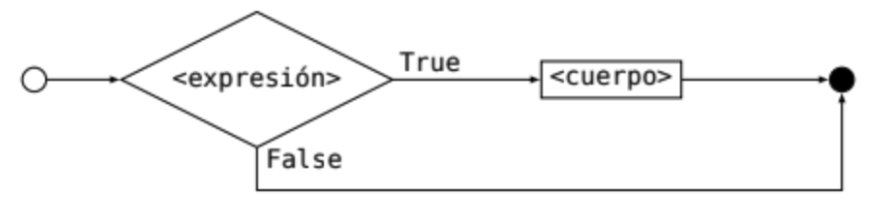
\includegraphics{imgs/unidad_3/if.png}

}

\caption{Diagrama de Flujo para la instrucción \texttt{if}}

\end{figure}%

Como ahora ya sabemos cómo construir condiciones de comparación, vamos a
comparar si nuestro número \texttt{x} es mayor a \texttt{0}:

\begin{Shaded}
\begin{Highlighting}[]
\KeywordTok{def}\NormalTok{ imprimir\_si\_positivo(x):}
  \ControlFlowTok{if}\NormalTok{ x }\OperatorTok{\textgreater{}} \DecValTok{0}\NormalTok{:}
      \BuiltInTok{print}\NormalTok{(}\StringTok{"Número positivo"}\NormalTok{)}
\end{Highlighting}
\end{Shaded}

Podemos probarlo:

\begin{Shaded}
\begin{Highlighting}[]
\NormalTok{imprimir\_si\_positivo(}\DecValTok{5}\NormalTok{)}
\NormalTok{imprimir\_si\_positivo(}\OperatorTok{{-}}\DecValTok{5}\NormalTok{)}
\NormalTok{imprimir\_si\_positivo(}\DecValTok{0}\NormalTok{)}
\end{Highlighting}
\end{Shaded}

\begin{verbatim}
Número positivo
\end{verbatim}

Como vemos, si el número es positivo, se imprime el mensaje. Pero si el
número no es positivo, no se imprime nada. Necesitamos además agregar un
mensaje ``Número no positivo'', si es que la condición no se cumple.

Modifiquemos el diseño: 1. Si \(x>0\), se imprime ``Número positivo''.
2. En caso contrario, se imprime ``Número no positivo''.

Podríamos probar con el siguiente código:

\begin{Shaded}
\begin{Highlighting}[]
\KeywordTok{def}\NormalTok{ imprimir\_si\_positivo(x):}
  \ControlFlowTok{if}\NormalTok{ x }\OperatorTok{\textgreater{}} \DecValTok{0}\NormalTok{:}
      \BuiltInTok{print}\NormalTok{(}\StringTok{"Número positivo"}\NormalTok{)}
  \ControlFlowTok{if} \KeywordTok{not}\NormalTok{ x }\OperatorTok{\textgreater{}} \DecValTok{0}\NormalTok{:}
      \BuiltInTok{print}\NormalTok{(}\StringTok{"Número no positivo"}\NormalTok{)}
\end{Highlighting}
\end{Shaded}

Otra solución posible es:

\begin{Shaded}
\begin{Highlighting}[]
\KeywordTok{def}\NormalTok{ imprimir\_si\_positivo(x):}
  \ControlFlowTok{if}\NormalTok{ x }\OperatorTok{\textgreater{}} \DecValTok{0}\NormalTok{:}
      \BuiltInTok{print}\NormalTok{(}\StringTok{"Número positivo"}\NormalTok{)}
  \ControlFlowTok{if}\NormalTok{ x }\OperatorTok{\textless{}=} \DecValTok{0}\NormalTok{:}
      \BuiltInTok{print}\NormalTok{(}\StringTok{"Número no positivo"}\NormalTok{)}
\end{Highlighting}
\end{Shaded}

Ambas están bien. Si lo probamos, vemos que funciona:

\begin{Shaded}
\begin{Highlighting}[]
\NormalTok{imprimir\_si\_positivo(}\DecValTok{5}\NormalTok{)}
\NormalTok{imprimir\_si\_positivo(}\OperatorTok{{-}}\DecValTok{5}\NormalTok{)}
\NormalTok{imprimir\_si\_positivo(}\DecValTok{0}\NormalTok{)}
\end{Highlighting}
\end{Shaded}

\begin{verbatim}
Número positivo
Número no positivo
Número no positivo
\end{verbatim}

Sin embargo, hay una mejor forma de hacer esta función. Existe una
condición alternativa para la estructura de decisión \texttt{if}, que
tiene la forma:

\begin{Shaded}
\begin{Highlighting}[]
\ControlFlowTok{if} \OperatorTok{\textless{}}\NormalTok{expresion}\OperatorTok{\textgreater{}}\NormalTok{:}
    \OperatorTok{\textless{}}\NormalTok{cuerpo}\OperatorTok{\textgreater{}}
\ControlFlowTok{else}\NormalTok{:}
    \OperatorTok{\textless{}}\NormalTok{cuerpo}\OperatorTok{\textgreater{}}
\end{Highlighting}
\end{Shaded}

donde \texttt{if} y \texttt{else} son palabras reservadas. Su efecto es
el siguiente:

\begin{enumerate}
\def\labelenumi{\arabic{enumi}.}
\tightlist
\item
  Se evalúa la \texttt{\textless{}expresion\textgreater{}}.
\item
  Si la \texttt{\textless{}expresion\textgreater{}} es verdadera, se
  ejecuta el \texttt{\textless{}cuerpo\textgreater{}} del \texttt{if}.
\item
  Si la \texttt{\textless{}expresion\textgreater{}} es falsa, se ejecuta
  el \texttt{\textless{}cuerpo\textgreater{}} del \texttt{else}.
\end{enumerate}

\begin{figure}[H]

{\centering 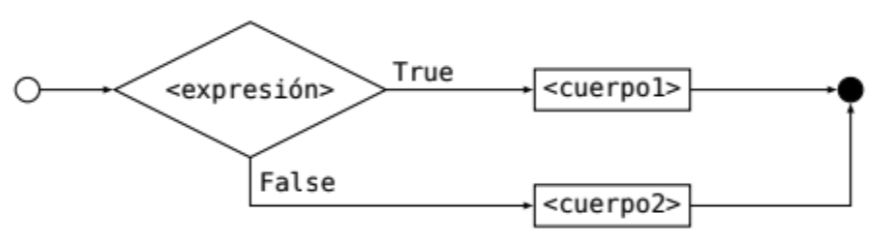
\includegraphics{imgs/unidad_3/if-else.png}

}

\caption{Diagrama de Flujo para la instrucción \texttt{if-else}}

\end{figure}%

Por lo tanto, podemos reescribir nuestra función de la siguiente forma:

\begin{Shaded}
\begin{Highlighting}[]
\KeywordTok{def}\NormalTok{ imprimir\_si\_positivo\_o\_no(x): }\CommentTok{\# le cambiamos el nombre}
  \ControlFlowTok{if}\NormalTok{ x }\OperatorTok{\textgreater{}} \DecValTok{0}\NormalTok{:}
      \BuiltInTok{print}\NormalTok{(}\StringTok{"Número positivo"}\NormalTok{)}
  \ControlFlowTok{else}\NormalTok{:}
      \BuiltInTok{print}\NormalTok{(}\StringTok{"Número no positivo"}\NormalTok{)}
\end{Highlighting}
\end{Shaded}

Probemos:

\begin{Shaded}
\begin{Highlighting}[]
\NormalTok{imprimir\_si\_positivo\_o\_no(}\DecValTok{5}\NormalTok{)}
\NormalTok{imprimir\_si\_positivo\_o\_no(}\OperatorTok{{-}}\DecValTok{5}\NormalTok{)}
\NormalTok{imprimir\_si\_positivo\_o\_no(}\DecValTok{0}\NormalTok{)}
\end{Highlighting}
\end{Shaded}

\begin{verbatim}
Número positivo
Número no positivo
Número no positivo
\end{verbatim}

¡Sigue funcionando!

Lo importante a destacar es que, si la condición del \texttt{if} es
verdadera, se ejecuta el \texttt{\textless{}cuerpo\textgreater{}} del
\texttt{if} y \textbf{no} se ejecuta el
\texttt{\textless{}cuerpo\textgreater{}} del \texttt{else}. Y viceversa:
si la condición del \texttt{if} es falsa, se ejecuta el
\texttt{\textless{}cuerpo\textgreater{}} del \texttt{else} y \textbf{no}
se ejecuta el \texttt{\textless{}cuerpo\textgreater{}} del \texttt{if}.
Nunca se ejecutan ambos casos, porque son caminos paralelos que no se
cruzan, como vimos en el diagrama de flujo más arriba.

\subsection{Múltiples decisiones
consecutivas.}\label{muxfaltiples-decisiones-consecutivas.}

Supongamos que ahora queremos imprimir un mensaje distinto si el número
es positivo, negativo o cero. Podríamos hacerlo con dos decisiones
consecutivas:

\begin{Shaded}
\begin{Highlighting}[]
\KeywordTok{def}\NormalTok{ imprimir\_si\_positivo\_negativo\_o\_cero(x):}
  \ControlFlowTok{if}\NormalTok{ x }\OperatorTok{\textgreater{}} \DecValTok{0}\NormalTok{:}
      \BuiltInTok{print}\NormalTok{(}\StringTok{"Número positivo"}\NormalTok{) }\CommentTok{\# cuerpo del primer if}
  \ControlFlowTok{else}\NormalTok{:}
      \ControlFlowTok{if}\NormalTok{ x }\OperatorTok{==} \DecValTok{0}\NormalTok{:                      }\CommentTok{\#}
          \BuiltInTok{print}\NormalTok{(}\StringTok{"Número cero"}\NormalTok{)        }\CommentTok{\#}
      \ControlFlowTok{else}\NormalTok{:                           }\CommentTok{\#}
          \BuiltInTok{print}\NormalTok{(}\StringTok{"Número negativo"}\NormalTok{)    }\CommentTok{\# todo esto es el cuerpo del primer else}
\end{Highlighting}
\end{Shaded}

A esto se le llama \emph{anidar}, y es donde dentro de unas ramas de la
decisión (en este caso, la del \texttt{else}), se anida una nueva
decisión. Pero no es la única forma de implementarlo. Podríamos hacerlo
de la siguiente forma:

\begin{Shaded}
\begin{Highlighting}[]
\KeywordTok{def}\NormalTok{ imprimir\_si\_positivo\_negativo\_o\_cero(x):}
  \ControlFlowTok{if}\NormalTok{ x }\OperatorTok{\textgreater{}} \DecValTok{0}\NormalTok{:}
      \BuiltInTok{print}\NormalTok{(}\StringTok{"Número positivo"}\NormalTok{)}
  \ControlFlowTok{elif}\NormalTok{ x }\OperatorTok{==} \DecValTok{0}\NormalTok{:}
      \BuiltInTok{print}\NormalTok{(}\StringTok{"Número cero"}\NormalTok{)}
  \ControlFlowTok{else}\NormalTok{:}
      \BuiltInTok{print}\NormalTok{(}\StringTok{"Número negativo"}\NormalTok{)}
\end{Highlighting}
\end{Shaded}

La estructura \texttt{elif} es una abreviatura de \texttt{else\ if}. Es
decir, es un \texttt{else} que tiene una condición. Su efecto es el
siguiente:

\begin{figure}[H]

{\centering 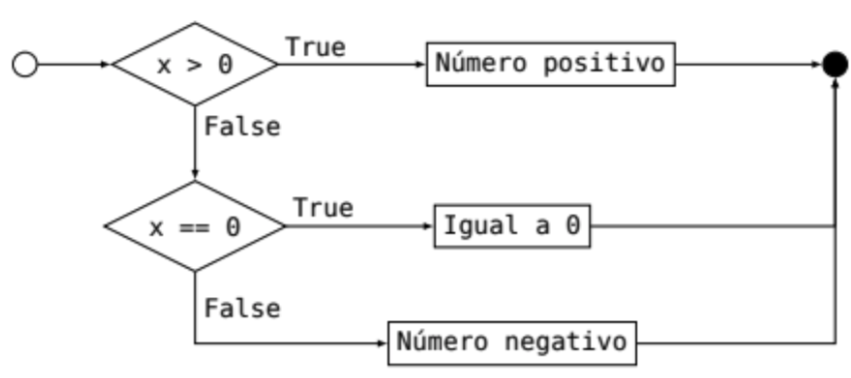
\includegraphics{imgs/unidad_3/if-elif-else.png}

}

\caption{Diagrama de Flujo para la instrucción \texttt{if-elif-else} del
ejemplo}

\end{figure}%

\begin{enumerate}
\def\labelenumi{\arabic{enumi}.}
\tightlist
\item
  Se evalúa la \texttt{\textless{}expresion\textgreater{}} del
  \texttt{if}.
\item
  Si la \texttt{\textless{}expresion\textgreater{}} es verdadera, se
  ejecuta el \texttt{\textless{}cuerpo\textgreater{}} del \texttt{if}.
\item
  Si la \texttt{\textless{}expresion\textgreater{}} es falsa, se evalúa
  la \texttt{\textless{}expresion\textgreater{}} del \texttt{elif}.
\item
  Si la \texttt{\textless{}expresion\textgreater{}} del \texttt{elif} es
  verdadera, se ejecuta su \texttt{\textless{}cuerpo\textgreater{}}.
\item
  Si la \texttt{\textless{}expresion\textgreater{}} del \texttt{elif} es
  falsa, se ejecuta el \texttt{\textless{}cuerpo\textgreater{}} del
  \texttt{else}.
\end{enumerate}

\begin{tcolorbox}[enhanced jigsaw, bottomrule=.15mm, leftrule=.75mm, opacityback=0, colback=white, toprule=.15mm, bottomtitle=1mm, opacitybacktitle=0.6, rightrule=.15mm, left=2mm, arc=.35mm, coltitle=black, title=\textcolor{quarto-callout-tip-color}{\faLightbulb}\hspace{0.5em}{Sabías que\ldots{} ?}, breakable, toptitle=1mm, colframe=quarto-callout-tip-color-frame, titlerule=0mm, colbacktitle=quarto-callout-tip-color!10!white]

En Python se consideran \emph{verdaderos} (True) también todos los
valores numéricos distintos de 0, las cadenas de caracteres que no sean
vacías, y cualquier valor que no sea vacío en general. Los valores nulos
o vacíos son \emph{falsos}.

\begin{Shaded}
\begin{Highlighting}[]
\ControlFlowTok{if}\NormalTok{ x }\OperatorTok{==} \DecValTok{0}\NormalTok{:}
\end{Highlighting}
\end{Shaded}

es equivalente a:

\begin{Shaded}
\begin{Highlighting}[]
\ControlFlowTok{if} \KeywordTok{not}\NormalTok{ x:}
\end{Highlighting}
\end{Shaded}

Y además, existe el valor especial \textbf{\texttt{None}}, que
representa la ausencia de valor, y es considerado \emph{falso}. Podemos
preguntar si una variable tiene el valor \texttt{None} usando el
operador \texttt{is}:

\begin{Shaded}
\begin{Highlighting}[]
\ControlFlowTok{if}\NormalTok{ x }\KeywordTok{is} \VariableTok{None}\NormalTok{:}
\end{Highlighting}
\end{Shaded}

o también:

\begin{Shaded}
\begin{Highlighting}[]
\ControlFlowTok{if} \KeywordTok{not}\NormalTok{ x:}
\end{Highlighting}
\end{Shaded}

\end{tcolorbox}

\begin{tcolorbox}[enhanced jigsaw, bottomrule=.15mm, leftrule=.75mm, opacityback=0, colback=white, toprule=.15mm, bottomtitle=1mm, opacitybacktitle=0.6, rightrule=.15mm, left=2mm, arc=.35mm, coltitle=black, title=\textcolor{quarto-callout-important-color}{\faExclamation}\hspace{0.5em}{Ejercicio Desafío}, breakable, toptitle=1mm, colframe=quarto-callout-important-color-frame, titlerule=0mm, colbacktitle=quarto-callout-important-color!10!white]

Debemos calcular el pago de una persona empleada en nuestra empresa. El
cálculo debe hacerse por la cantidad de horas trabajadas, y se le debe
pedir al usuario la cantidad de horas y cuánto vale cada hora.\\
Adicionalmente, se abona un plus fijo de guardería a todo empleado/a con
infantes a su cargo. Y se paga un 10\% de incentivo a todo empleado/a
que haya trabajado 30 horas o más y \textbf{no} reciba el plus por
guardería.\\

Pista: pensar los distintos tipos de liquidación:\\
a) Empleado/a con menos de 30 horas y sin infantes a cargo.\\
b) Empleado/a con 30 horas o más y sin infantes a cargo.\\
c) Empleado/a con menos de 30 horas y con infantes a cargo.\\
d) Empleado/a con 30 horas o más y con infantes a cargo.

\begin{tcolorbox}[enhanced jigsaw, bottomrule=.15mm, leftrule=.75mm, opacityback=0, colback=white, toprule=.15mm, bottomtitle=1mm, opacitybacktitle=0.6, rightrule=.15mm, left=2mm, arc=.35mm, coltitle=black, title=\textcolor{quarto-callout-tip-color}{\faLightbulb}\hspace{0.5em}{Ayuda: Flujo de la resolución}, breakable, toptitle=1mm, colframe=quarto-callout-tip-color-frame, titlerule=0mm, colbacktitle=quarto-callout-tip-color!10!white]

\begin{figure}[H]

{\centering 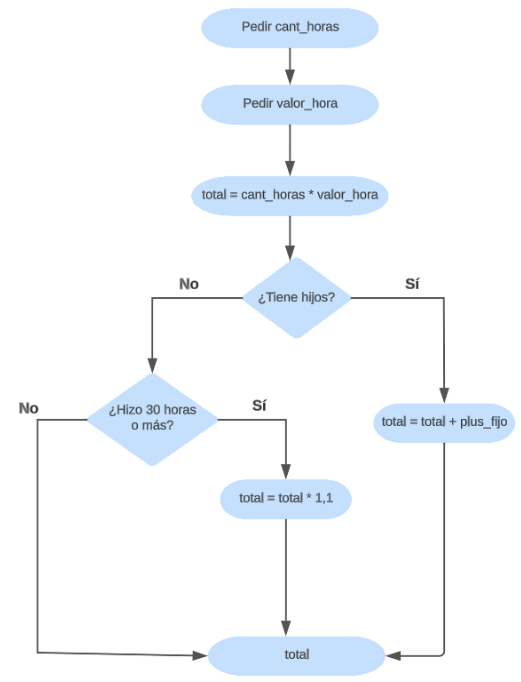
\includegraphics{imgs/unidad_3/flujo-desafio.png}

}

\caption{Diagrama de Flujo para el desafío}

\end{figure}%

\end{tcolorbox}

\end{tcolorbox}

\section{Ciclos y Rangos}\label{ciclos-y-rangos}

Supongamos que en una fábrica se nos pide hacer un procedimiento para
entrenar al personal nuevo. Para comenzar se nos encarga la descripción
de uno muy simple: descarga de cajas de material del camión del
proveedor y almacenamiento en el depósito. Así que aplicamos lo que
venimos aprendiendo hasta ahora sobre algoritmos y describimos la
operación para la descarga de 3 cajas:

\begin{verbatim}
1 Abrir la puerta del depósito y encender luces 
2 Ir al garage o playón donde estacionó el camión 
3 Abrir las puertas traseras de la caja del transporte

4 Tomar una caja con ambas manos, asegurándola para no tirarla 
5 Caminar sosteniendo la caja hasta el depósito 
6 Colocar la caja sobre el piso en el sector correspondiente 
7 Ir al garage o playón donde estacionó el camión

8 Tomar OTRA caja con ambas manos, asegurándola para no tirarla 
9 Caminar sosteniendo la caja hasta el depósito 
10 Colocar la caja sobre la caja anterior 
11 Ir al garage o playón donde estacionó el camión

12 Tomar OTRA caja con ambas manos, asegurándola para no tirarla 
13 Caminar sosteniendo la caja hasta el depósito 
14 Colocar la caja sobre la caja anterior

15 Apagar luces y cerrar puerta del depósito 
16 Ir al garage o playón donde estacionó el camión 
17 Cerrar y trabar puertas del camión 
18 Avisar fin de descarga al transportista
\end{verbatim}

Ya lo tenemos. Ahora la persona a cargo dice que en el camión suelen
venir entre 5 y 15 cajas de material y pide que definas el mismo
procedimiento para todos los casos posibles. Notemos que se repiten las
instrucciones 2, 3, 4, 5 y 6 para cada caja ¿Qué hacemos? ¿Vamos a
seguir copiando y pegando las instrucciones para cada caja? ¿Y si algún
día vienen más de 15 o menos de 5? ¿Vamos a tener una lista de
instrucciones distinta para cada cantidad de cajas que puedan venir?
Parece ser necesario hacer algo más genérico que le facilite la vida a
todos. Una nueva versión:

\begin{verbatim}
1 Abrir la puerta del depósito y encender luces 
2 Ir al garage o playón donde estacionó el camión 
3 Abrir las puertas traseras de la caja del transporte 
4 Tomar una caja con ambas manos, asegurándola para no tirarla 
5 Caminar sosteniendo la caja hasta el depósito 
6 Si es la primera caja, colocarla sobre el piso en el sector correspondiente;
si no, apilarla sobre la anterior;
salvo que ya haya 3 apiladas,
en ese caso colocarla a la derecha sobre el piso 
7 Ir al garage o playón donde estacionó el camión 

8 Repetir 4,5,6,7 mientras queden cajas para descargar 

9 Cerrar y trabar puertas del camión 
10 Avisar fin de descarga al transportista 
11 Volver a depósito 
12 Apagar luces y cerrar puerta del depósito
\end{verbatim}

Esta descripción es bastante más compacta y cubre todas las posibles
cantidades de cajas en un envío (habituales y excepcionales), de modo
que con una única página en el manual de procedimientos será suficiente.

Sin embargo, los algoritmos que venimos escribiendo se parecen más al
primer procedimiento que al segundo. ¿Cómo podemos mejorarlos?

\begin{tcolorbox}[enhanced jigsaw, bottomrule=.15mm, leftrule=.75mm, opacityback=0, colback=white, toprule=.15mm, bottomtitle=1mm, opacitybacktitle=0.6, rightrule=.15mm, left=2mm, arc=.35mm, coltitle=black, title=\textcolor{quarto-callout-note-color}{\faInfo}\hspace{0.5em}{Ciclos}, breakable, toptitle=1mm, colframe=quarto-callout-note-color-frame, titlerule=0mm, colbacktitle=quarto-callout-note-color!10!white]

El \textbf{ciclo}, \textbf{bucle} o \textbf{sentencia iterativa} es una
instrucción que permite ejecutar un bloque de código varias veces. En
Python, existen dos tipos de ciclos: \texttt{while} y \texttt{for}.

\end{tcolorbox}

\subsection{\texorpdfstring{Ciclo
\texttt{for}}{Ciclo for}}\label{ciclo-for}

La instrucción \texttt{for} nos indica que queremos repetir un bloque de
código una cierta cantidad de veces. Por ejemplo, si queremos imprimir
los números del 1 al 10, podemos hacerlo de la siguiente forma:

\begin{Shaded}
\begin{Highlighting}[]
\ControlFlowTok{for}\NormalTok{ i }\KeywordTok{in} \BuiltInTok{range}\NormalTok{(}\DecValTok{1}\NormalTok{, }\DecValTok{11}\NormalTok{):}
    \BuiltInTok{print}\NormalTok{(i)}
\end{Highlighting}
\end{Shaded}

\begin{verbatim}
1
2
3
4
5
6
7
8
9
10
\end{verbatim}

El ciclo \texttt{for} incluye una línea de \emph{inicialización} y una
línea de \texttt{\textless{}cuerpo\textgreater{}}, que puede tener una o
más instrucciones. El ciclo definido es de la forma:

\begin{Shaded}
\begin{Highlighting}[]
\ControlFlowTok{for} \OperatorTok{\textless{}}\NormalTok{nombre}\OperatorTok{\textgreater{}} \KeywordTok{in} \OperatorTok{\textless{}}\NormalTok{expresion}\OperatorTok{\textgreater{}}\NormalTok{:}
    \OperatorTok{\textless{}}\NormalTok{cuerpo}\OperatorTok{\textgreater{}}
\end{Highlighting}
\end{Shaded}

El ciclo se dice \emph{definido} porque una vez evaluada la
\texttt{\textless{}expresion\textgreater{}}, se sabe cuántas veces se va
a ejecutar el \texttt{\textless{}cuerpo\textgreater{}}: tantas veces
como elementos tenga la \texttt{\textless{}expresion\textgreater{}}.

La expresión puede indicarse con \texttt{range}:

\begin{itemize}
\tightlist
\item
  \texttt{range(n)} devuelve una secuencia de números desde 0 hasta
  \texttt{n-1}.
\item
  \texttt{range(a,\ b)} devuelve una secuencia de números desde
  \texttt{a} hasta \texttt{b-1}.
\item
  \texttt{range(a,\ b,\ c)} devuelve una secuencia de números desde
  \texttt{a} hasta \texttt{b-1}, de a \texttt{c} en \texttt{c}.
\end{itemize}

Se podría decir que el \texttt{range} puede recibir 3 valores:
\texttt{range(start,\ end,\ step)} o
\texttt{range(inicio,\ fin,\ paso)}, donde:

\begin{itemize}
\tightlist
\item
  \texttt{start} o \texttt{inicio} es el valor inicial de la secuencia.
  Por defecto es 0.
\item
  \texttt{end} o \texttt{fin} es el valor final de la secuencia.
  \textbf{No} se incluye en la secuencia.
\item
  \texttt{step} o \texttt{paso} es el incremento entre cada elemento de
  la secuencia. Por defecto es 1.
\end{itemize}

Si le pasamos un sólo parámetro, lo toma como \texttt{end}.\\
Si le pasamos dos, los toma como \texttt{start} y \texttt{end}.\\
Y si le pasamos tres, los toma como \texttt{start}, \texttt{end} y
\texttt{step}.

\begin{tcolorbox}[enhanced jigsaw, bottomrule=.15mm, leftrule=.75mm, opacityback=0, colback=white, toprule=.15mm, bottomtitle=1mm, opacitybacktitle=0.6, rightrule=.15mm, left=2mm, arc=.35mm, coltitle=black, title=\textcolor{quarto-callout-note-color}{\faInfo}\hspace{0.5em}{Note}, breakable, toptitle=1mm, colframe=quarto-callout-note-color-frame, titlerule=0mm, colbacktitle=quarto-callout-note-color!10!white]

¿Te suena quizás a algo que ya vimos? Quizás\ldots{} ¿los \emph{slices}
de las cadenas de caracteres?

\end{tcolorbox}

Además, la variable \texttt{\textless{}nombre\textgreater{}} va a ir
tomando el valor de cada elemento de la
\texttt{\textless{}expresion\textgreater{}} en cada iteración. En
nuestro ejemplo de imprimir los números del 1 al 10, vemos que i toma
los valores 1, 2, 3, 4, 5, 6, 7, 8, 9 y 10, en ese orden.\\

\begin{quote}
\textbf{Ejemplo}\\
Se pide una función que imprima todos los números pares entre dos
números dados \texttt{a} y \texttt{b}. Se considera que \texttt{a} y
\texttt{b} son siempre números enteros positivos, y que \texttt{a} es
menor que \texttt{b}.
\end{quote}

\begin{Shaded}
\begin{Highlighting}[]
\KeywordTok{def}\NormalTok{ imprimir\_pares(a, b):}
  \ControlFlowTok{for}\NormalTok{ i }\KeywordTok{in} \BuiltInTok{range}\NormalTok{(a, b):}
    \ControlFlowTok{if}\NormalTok{ i }\OperatorTok{\%} \DecValTok{2} \OperatorTok{==} \DecValTok{0}\NormalTok{: }\CommentTok{\# si el resto de dividir por 2 es cero, es par}
      \BuiltInTok{print}\NormalTok{(i)}

\NormalTok{imprimir\_pares(}\DecValTok{1}\NormalTok{,}\DecValTok{15}\NormalTok{)}
\end{Highlighting}
\end{Shaded}

\begin{verbatim}
2
4
6
8
10
12
14
\end{verbatim}

\hfill\break

\begin{quote}
\textbf{Ejemplo}\\
Se pide una función que imprima todos los números del 1 al 10, en orden
inverso.
\end{quote}

\begin{Shaded}
\begin{Highlighting}[]
\KeywordTok{def}\NormalTok{ imprimir\_inverso():}
  \ControlFlowTok{for}\NormalTok{ i }\KeywordTok{in} \BuiltInTok{range}\NormalTok{(}\DecValTok{10}\NormalTok{, }\DecValTok{0}\NormalTok{, }\OperatorTok{{-}}\DecValTok{1}\NormalTok{):}
      \BuiltInTok{print}\NormalTok{(i)}

\NormalTok{imprimir\_inverso()}
\end{Highlighting}
\end{Shaded}

\begin{verbatim}
10
9
8
7
6
5
4
3
2
1
\end{verbatim}

\hfill\break

\subsubsection{Iterables}\label{iterables}

Como dijimos más arriba, la expresión del \texttt{for} puede ser
cualquier expresión que devuelva una secuencia de valores. A estas
expresiones se las llama \emph{iterables}.

Un ciclo \texttt{for} también podría iterar sobre elementos de una lista
(tema que vamos a ver más adelante), o sobre caracteres de una palabra.
Por ejemplo:

\begin{Shaded}
\begin{Highlighting}[]
\ControlFlowTok{for}\NormalTok{ num }\KeywordTok{in}\NormalTok{ [}\DecValTok{1}\NormalTok{, }\DecValTok{3}\NormalTok{, }\DecValTok{7}\NormalTok{, }\DecValTok{5}\NormalTok{, }\DecValTok{2}\NormalTok{]:}
    \BuiltInTok{print}\NormalTok{(num)}
\end{Highlighting}
\end{Shaded}

\begin{verbatim}
1
3
7
5
2
\end{verbatim}

\begin{Shaded}
\begin{Highlighting}[]
\ControlFlowTok{for}\NormalTok{ c }\KeywordTok{in} \StringTok{"Hola"}\NormalTok{:}
    \BuiltInTok{print}\NormalTok{(c)}
\end{Highlighting}
\end{Shaded}

\begin{verbatim}
H
o
l
a
\end{verbatim}

\subsection{\texorpdfstring{Ciclo
\texttt{while}}{Ciclo while}}\label{ciclo-while}

La instrucción \texttt{while} nos indica que queremos repetir un bloque
de código \emph{mientras} se cumpla una condición. Por ejemplo, si
queremos imprimir los números del 1 al 10, podemos hacerlo de la
siguiente forma:

\begin{Shaded}
\begin{Highlighting}[]
\NormalTok{i }\OperatorTok{=} \DecValTok{1}
\ControlFlowTok{while}\NormalTok{ i }\OperatorTok{\textless{}} \DecValTok{11}\NormalTok{:}
    \BuiltInTok{print}\NormalTok{(i)}
\NormalTok{    i }\OperatorTok{+=} \DecValTok{1}
\end{Highlighting}
\end{Shaded}

\begin{verbatim}
1
2
3
4
5
6
7
8
9
10
\end{verbatim}

El ciclo \texttt{while} incluye una línea de \emph{inicialización} y una
línea de \texttt{\textless{}cuerpo\textgreater{}}, que puede tener una o
más instrucciones. El ciclo definido es de la forma:

\begin{Shaded}
\begin{Highlighting}[]
\ControlFlowTok{while} \OperatorTok{\textless{}}\NormalTok{expresion}\OperatorTok{\textgreater{}}\NormalTok{:}
    \OperatorTok{\textless{}}\NormalTok{cuerpo}\OperatorTok{\textgreater{}}
\end{Highlighting}
\end{Shaded}

El ciclo se dice \emph{indefinido} porque una vez evaluada la
\texttt{\textless{}expresion\textgreater{}}, \textbf{no} se sabe cuántas
veces se va a ejecutar el \texttt{\textless{}cuerpo\textgreater{}}: se
ejecuta mientras la \texttt{\textless{}expresion\textgreater{}} sea
verdadera.

Para usar la instrucción \texttt{while}, tenemos cuatro aspectos para
armar y afinar correctamente:

\begin{itemize}
\tightlist
\item
  Cuerpo
\item
  Condición
\item
  Estado Previo
\item
  Paso
\end{itemize}

Antes, para la instrucción \texttt{for}, sólo considerábamos el cuerpo y
la condición. Ahora, además, tenemos que considerar el estado previo y
el paso.

El \textbf{cuerpo} es la porción de código que se repetirá mientras la
condición sea verdadera.\\
La \textbf{condición} es la expresión booleana que se evalúa para
decidir si se ejecuta el cuerpo o no.\\
El \textbf{estado previo} es el estado de las variables antes de
ejecutar el cuerpo. En general, se refiere al estado de las variables
que participan de la condición.\\
El \textbf{paso} es la porción de código que modifica el estado previo.
En general, se refiere a la modificación de las variables que participan
de la condición.\\

\begin{tcolorbox}[enhanced jigsaw, bottomrule=.15mm, leftrule=.75mm, opacityback=0, colback=white, toprule=.15mm, bottomtitle=1mm, opacitybacktitle=0.6, rightrule=.15mm, left=2mm, arc=.35mm, coltitle=black, title=\textcolor{quarto-callout-warning-color}{\faExclamationTriangle}\hspace{0.5em}{Warning}, breakable, toptitle=1mm, colframe=quarto-callout-warning-color-frame, titlerule=0mm, colbacktitle=quarto-callout-warning-color!10!white]

Con los ciclos \texttt{while} hay que tener mucho cuidado de no caer en
un loop infinito. Esto sucede cuando la condición siempre es verdadera,
y el cuerpo no modifica el estado previo. Por ejemplo:

\begin{Shaded}
\begin{Highlighting}[]
\ControlFlowTok{while} \VariableTok{True}\NormalTok{: }\CommentTok{\# más adelante sobre el uso de \textasciigrave{}while True\textasciigrave{}}
    \BuiltInTok{print}\NormalTok{(}\StringTok{"Hola"}\NormalTok{)}
\end{Highlighting}
\end{Shaded}

o bien:

\begin{Shaded}
\begin{Highlighting}[]
\NormalTok{i }\OperatorTok{=} \DecValTok{0}
\ControlFlowTok{while}\NormalTok{ i }\OperatorTok{\textless{}} \DecValTok{10}\NormalTok{:}
    \BuiltInTok{print}\NormalTok{(i) }\CommentTok{\# el valor de i nunca cambia}
\end{Highlighting}
\end{Shaded}

\end{tcolorbox}

\begin{quote}
\textbf{Ejercicio}\\
Repetir el ejercicio 7.b de la guía 2 usando un ciclo \texttt{while}.
Repetir usando un ciclo \texttt{for}. ¿Qué diferencias hay entre ambos?
~
\end{quote}

\subsection{Break, Continue y Return}\label{break-continue-y-return}

\texttt{break} y \texttt{continue}son dos palabras clave en Python que
se utilizan en bucles (tanto \texttt{for} como \texttt{while}) para
alterar el flujo de ejecución del bucle.

\subsubsection{Break}\label{break}

La declaración \texttt{break} se usa para salir inmediatamente de un
bucle antes de que se complete su iteración normal. Cuando se encuentra
una declaración \texttt{break} dentro de un bucle, el bucle \texttt{for}
o \texttt{while} se detiene inmediatamente y continúa con la ejecución
de las instrucciones que están después del mismo.

Por ejemplo, supongamos que queremos encontrar al primer número múltiplo
de 3 entre 10 y 30:

\begin{Shaded}
\begin{Highlighting}[]
\NormalTok{numero }\OperatorTok{=} \DecValTok{10}
\ControlFlowTok{while}\NormalTok{ numero }\OperatorTok{\textless{}=} \DecValTok{30}\NormalTok{:}
  \ControlFlowTok{if}\NormalTok{ numero }\OperatorTok{\%} \DecValTok{3} \OperatorTok{==} \DecValTok{0}\NormalTok{:}
      \BuiltInTok{print}\NormalTok{(}\StringTok{"El primer número múltiplo de 3 es:"}\NormalTok{, numero)}
      \ControlFlowTok{break}
\NormalTok{  numero }\OperatorTok{+=} \DecValTok{1}
\end{Highlighting}
\end{Shaded}

\begin{verbatim}
El primer número múltiplo de 3 es: 12
\end{verbatim}

\begin{Shaded}
\begin{Highlighting}[]
\ControlFlowTok{for}\NormalTok{ numero }\KeywordTok{in} \BuiltInTok{range}\NormalTok{(}\DecValTok{10}\NormalTok{, }\DecValTok{31}\NormalTok{):}
  \ControlFlowTok{if}\NormalTok{ numero }\OperatorTok{\%} \DecValTok{3} \OperatorTok{==} \DecValTok{0}\NormalTok{:}
      \BuiltInTok{print}\NormalTok{(}\StringTok{"El primer número múltiplo de 3 es:"}\NormalTok{, numero)}
      \ControlFlowTok{break}
\end{Highlighting}
\end{Shaded}

\begin{verbatim}
El primer número múltiplo de 3 es: 12
\end{verbatim}

\subsubsection{Continue}\label{continue}

La declaración \texttt{continue} se usa para omitir el resto del código
dentro de una iteración actual del bucle y continuar con la siguiente
iteración. Cuando se encuentra una declaración \texttt{continue} dentro
de un bucle, el bucle \texttt{for} o \texttt{while} salta a la siguiente
iteración del bucle sin ejecutar las instrucciones que están después del
\texttt{continue}.

Por ejemplo, supongamos que queremos imprimir todos los números entre 1
y 20, excepto los múltiplos de 4:

\begin{Shaded}
\begin{Highlighting}[]
\NormalTok{numero }\OperatorTok{=} \DecValTok{1}
\ControlFlowTok{while}\NormalTok{ numero }\OperatorTok{\textless{}=} \DecValTok{20}\NormalTok{:}
  \ControlFlowTok{if}\NormalTok{ numero }\OperatorTok{\%} \DecValTok{4} \OperatorTok{==} \DecValTok{0}\NormalTok{:}
\NormalTok{      numero }\OperatorTok{+=} \DecValTok{1}
      \ControlFlowTok{continue}
  \BuiltInTok{print}\NormalTok{(numero)}
\NormalTok{  numero }\OperatorTok{+=} \DecValTok{1}
\end{Highlighting}
\end{Shaded}

\begin{verbatim}
1
2
3
5
6
7
9
10
11
13
14
15
17
18
19
\end{verbatim}

\begin{Shaded}
\begin{Highlighting}[]
\ControlFlowTok{for}\NormalTok{ numero }\KeywordTok{in} \BuiltInTok{range}\NormalTok{(}\DecValTok{1}\NormalTok{, }\DecValTok{21}\NormalTok{):}
  \ControlFlowTok{if}\NormalTok{ numero }\OperatorTok{\%} \DecValTok{4} \OperatorTok{==} \DecValTok{0}\NormalTok{:}
      \ControlFlowTok{continue}
  \BuiltInTok{print}\NormalTok{(numero)}
\end{Highlighting}
\end{Shaded}

\begin{verbatim}
1
2
3
5
6
7
9
10
11
13
14
15
17
18
19
\end{verbatim}

\begin{tcolorbox}[enhanced jigsaw, bottomrule=.15mm, leftrule=.75mm, opacityback=0, colback=white, toprule=.15mm, bottomtitle=1mm, opacitybacktitle=0.6, rightrule=.15mm, left=2mm, arc=.35mm, coltitle=black, title=\textcolor{quarto-callout-note-color}{\faInfo}\hspace{0.5em}{Note}, breakable, toptitle=1mm, colframe=quarto-callout-note-color-frame, titlerule=0mm, colbacktitle=quarto-callout-note-color!10!white]

Notemos que tanto para el uso de \texttt{break} como de
\texttt{continue}, si el código se encuentra con uno de ellos en la
ejecución, no ejecuta nada posterior a ellos: en el caso de
\texttt{break}, corta o interrumpe la ejecución del bucle; en el case de
\texttt{continue}, saltea el resto del código de esa iteración y pasa a
la siguiente, volviendo a evaluar la condición si el bucle es
\texttt{while}.

\end{tcolorbox}

\subsubsection{Return}\label{return}

Cuando estamos dentro de una función, la instrucción \texttt{return} nos
permite devolver un valor y salir de la función. Ahora, si además
estamos dentro de un ciclo, también nos permite salir del mismo sin
ejecutar el resto del código.

Por ejemplo:

\begin{Shaded}
\begin{Highlighting}[]
\KeywordTok{def}\NormalTok{ obtener\_primer\_par\_desde(n):}
  \ControlFlowTok{for}\NormalTok{ num }\KeywordTok{in} \BuiltInTok{range}\NormalTok{(n, n}\OperatorTok{+}\DecValTok{10}\NormalTok{):}
    \BuiltInTok{print}\NormalTok{(}\SpecialStringTok{f"Analizando si el número }\SpecialCharTok{\{}\NormalTok{num}\SpecialCharTok{\}}\SpecialStringTok{ es par"}\NormalTok{)}
    \ControlFlowTok{if}\NormalTok{ num }\OperatorTok{\%} \DecValTok{2} \OperatorTok{==} \DecValTok{0}\NormalTok{:}
      \ControlFlowTok{return}\NormalTok{ num}
  \ControlFlowTok{return} \VariableTok{None}
\end{Highlighting}
\end{Shaded}

\begin{Shaded}
\begin{Highlighting}[]
\NormalTok{obtener\_primer\_par\_desde(}\DecValTok{9}\NormalTok{)}
\end{Highlighting}
\end{Shaded}

\begin{verbatim}
Analizando si el número 9 es par
Analizando si el número 10 es par
\end{verbatim}

\begin{verbatim}
10
\end{verbatim}

Como vemos, la función \texttt{obtener\_primer\_par\_desde} recibe un
número \texttt{n}, y devuelve el primer número par que encuentra a
partir de \texttt{n}. Si no encuentra ningún número par, devuelve
\texttt{None}.\\
Si encuentra un número par, no sigue analizando el resto de los números.
Usa \texttt{return} para salir del ciclo y devuelve el número
encontrado.

\subsection{Consideraciones del While}\label{consideraciones-del-while}

Es importante \textbf{no} ser redundantes con el código y no ``hacer
preguntas'' que ya sabemos.

\begin{Shaded}
\begin{Highlighting}[]
\ControlFlowTok{while} \OperatorTok{\textless{}}\NormalTok{condicion}\OperatorTok{\textgreater{}}\NormalTok{:}
  \OperatorTok{\textless{}}\NormalTok{cuerpo}\OperatorTok{\textgreater{}}

\OperatorTok{\textless{}}\NormalTok{codigo cuando ya no se cumple la condición}\OperatorTok{\textgreater{}}
\end{Highlighting}
\end{Shaded}

Veamos un ejemplo:

\begin{Shaded}
\begin{Highlighting}[]
\NormalTok{numero }\OperatorTok{=} \DecValTok{0}
\ControlFlowTok{while}\NormalTok{ numero }\OperatorTok{\textless{}} \DecValTok{3}\NormalTok{:}
  \BuiltInTok{print}\NormalTok{(numero)}
\NormalTok{  numero }\OperatorTok{+=} \DecValTok{1}

\ControlFlowTok{if}\NormalTok{ numero }\OperatorTok{==} \DecValTok{3}\NormalTok{:}
  \BuiltInTok{print}\NormalTok{(}\StringTok{"El número es 3"}\NormalTok{)}
\ControlFlowTok{else}\NormalTok{:}
  \BuiltInTok{print}\NormalTok{(}\StringTok{"El número no es 3"}\NormalTok{)}
\end{Highlighting}
\end{Shaded}

El output va a ser siempre el mismo:

\begin{verbatim}
1
2
3
El número es 3
\end{verbatim}

¿Por qué? Porque nuestra condición del while es lo que dice
\emph{``mientras esto se cumpla, yo repito el bloque del código de
adentro''}. Nuestra condición es que \texttt{numero\ \textless{}\ 3}. En
el momento en que \texttt{numero} llega a 3, el bucle
\texttt{while}\textbf{deja} de cumplir con la condición, y la ejecución
se corta, se termina con el bucle.

Es decir, el bloque

\begin{Shaded}
\begin{Highlighting}[]
\ControlFlowTok{if}\NormalTok{ numero }\OperatorTok{==} \DecValTok{3}\NormalTok{:}
  \BuiltInTok{print}\NormalTok{(}\StringTok{"El número es 3"}\NormalTok{)}
\end{Highlighting}
\end{Shaded}

siempre se ejecuta.

Y el bloque

\begin{Shaded}
\begin{Highlighting}[]
\ControlFlowTok{else}\NormalTok{:}
  \BuiltInTok{print}\NormalTok{(}\StringTok{"El número no es 3"}\NormalTok{)}
\end{Highlighting}
\end{Shaded}

nunca se ejecuta.

Por lo tanto, podemos reescribir el código de la siguiente forma:

\begin{Shaded}
\begin{Highlighting}[]
\NormalTok{numero }\OperatorTok{=} \DecValTok{0}
\ControlFlowTok{while}\NormalTok{ numero }\OperatorTok{\textless{}} \DecValTok{3}\NormalTok{:}
  \BuiltInTok{print}\NormalTok{(numero)}
\NormalTok{  numero }\OperatorTok{+=} \DecValTok{1}

\BuiltInTok{print}\NormalTok{(}\StringTok{"El número es 3"}\NormalTok{)}
\end{Highlighting}
\end{Shaded}

\hfill\break
De la misma forma, no tendría sentido hacer algo así:

\begin{Shaded}
\begin{Highlighting}[]
\NormalTok{numero }\OperatorTok{=} \DecValTok{0} 
\ControlFlowTok{while}\NormalTok{ numero }\OperatorTok{\textless{}} \DecValTok{3}\NormalTok{:}
  \BuiltInTok{print}\NormalTok{(numero)}
\NormalTok{  numero }\OperatorTok{+=} \DecValTok{1}
  \ControlFlowTok{continue}

  \ControlFlowTok{if}\NormalTok{ numero }\OperatorTok{==} \DecValTok{3}\NormalTok{:}
    \ControlFlowTok{break}
\end{Highlighting}
\end{Shaded}

\begin{enumerate}
\def\labelenumi{\arabic{enumi}.}
\tightlist
\item
  \texttt{if\ numero\ ==\ 3} está absolutamente de más. Si
  \texttt{numero} es 3, el bucle \texttt{while} \textbf{no} se ejecuta,
  por lo que nunca se va a llegar a esa línea de código. No es necesario
  ``re-chequear'' la condición del while dentro del mismo, porque
  asumimos que si llegamos a esa línea de código, es porque la condición
  se cumplió. Por lo tanto, podemos reescribir el código de la siguiente
  forma:
\end{enumerate}

\begin{Shaded}
\begin{Highlighting}[]
\NormalTok{numero }\OperatorTok{=} \DecValTok{0} 
\ControlFlowTok{while}\NormalTok{ numero }\OperatorTok{\textless{}} \DecValTok{3}\NormalTok{:}
  \BuiltInTok{print}\NormalTok{(numero)}
\NormalTok{  numero }\OperatorTok{+=} \DecValTok{1}
  \ControlFlowTok{continue}
\end{Highlighting}
\end{Shaded}

\begin{enumerate}
\def\labelenumi{\arabic{enumi}.}
\setcounter{enumi}{1}
\tightlist
\item
  Ahora, el continue está de más también, porque se usa cuando nosotros
  queremos \emph{forzar} a que el ciclo pase a la siguiente iteración.
  Pero en este caso, el ciclo ya va a pasar a la siguiente iteración,
  porque estamos en la última línea del cuerpo.
\end{enumerate}

Este es nuestro código final, escrito de forma correcta:

\begin{Shaded}
\begin{Highlighting}[]
\NormalTok{numero }\OperatorTok{=} \DecValTok{0} 
\ControlFlowTok{while}\NormalTok{ numero }\OperatorTok{\textless{}} \DecValTok{3}\NormalTok{:}
  \BuiltInTok{print}\NormalTok{(numero)}
\NormalTok{  numero }\OperatorTok{+=} \DecValTok{1}
\end{Highlighting}
\end{Shaded}

\subsubsection{While True}\label{while-true}

La instrucción \texttt{while} está hecha para que se ejecute mientras la
condición sea verdadera. Pero, ¿qué pasa si usamos \texttt{while\ True}?
Lo que pasa al usar \texttt{while\ True} es que nuestro código se vuelve
más propenso al error: si no tenemos cuidado, podemos caer en un loop
infinito.\\

Como no tenemos una condición a evaluar ni modificar en cada iteración,
el bucle se ejecuta infinitamente. Dependería de nosotros, como
programadores, que el bucle se corte en algún momento. Es decir,
dependería de que nos acordemos de poner dentro del \texttt{while}
alguna decisión que haga que el bucle se corte. Y si por alguna razón no
nos acordamos, el bucle se ejecutaría infinitamente, dejando al programa
``congelado'' o ``colgado'', sin responder, y usando todos los recursos
de la computadora.

En pocas palabras, podemos afirmar que el uso de \texttt{while\ True} en
Python es una mala práctica de programación, y recomendamos evitarla
fuertemente.

\subsubsection{Modificando la
Condición}\label{modificando-la-condiciuxf3n}

\begin{Shaded}
\begin{Highlighting}[]
\ControlFlowTok{while} \OperatorTok{\textless{}}\NormalTok{condicion}\OperatorTok{\textgreater{}}\NormalTok{:}
  \OperatorTok{\textless{}}\NormalTok{cuerpo}\OperatorTok{\textgreater{}}
\end{Highlighting}
\end{Shaded}

La mejor decisión que se puede tomar para el de un bloque \texttt{while}
es asumir que, durante toda su ejecución exceptuando la última línea, la
condición se cumple. Es decir, que el cuerpo del bucle se ejecuta
mientras la condición sea verdadera. Por lo tanto, si queremos modificar
la condición, debemos hacerlo en la última línea del cuerpo.

Por ejemplo, esto no es correcto:

\begin{Shaded}
\begin{Highlighting}[]
\CommentTok{\# Se deben imprimir los números 0, 1, 2}
\NormalTok{numero }\OperatorTok{=} \DecValTok{0}
\ControlFlowTok{while}\NormalTok{ numero }\OperatorTok{\textless{}} \DecValTok{3}\NormalTok{:}
\NormalTok{  numero }\OperatorTok{+=} \DecValTok{1}     \CommentTok{\# actualización de la condición}
  \BuiltInTok{print}\NormalTok{(numero)}
\end{Highlighting}
\end{Shaded}

\begin{verbatim}
1
2
3
\end{verbatim}

Como vemos, se imprimen los números 1, 2, 3; pero no el 0. Esto es
porque estamos modificando la condición ni bien empieza el bucle, y no
en la última línea del cuerpo.

La forma correcta de hacerlo sería:

\begin{Shaded}
\begin{Highlighting}[]
\CommentTok{\# Se deben imprimir los números 0, 1, 2}
\NormalTok{numero }\OperatorTok{=} \DecValTok{0}
\ControlFlowTok{while}\NormalTok{ numero }\OperatorTok{\textless{}} \DecValTok{3}\NormalTok{:}
  \BuiltInTok{print}\NormalTok{(numero)}
\NormalTok{  numero }\OperatorTok{+=} \DecValTok{1}     \CommentTok{\# actualización de la condición}
\end{Highlighting}
\end{Shaded}

\begin{verbatim}
0
1
2
\end{verbatim}

De esta forma, todo lo que se encuentre antes de la última línea del
cuerpo se ejecuta mientras la condición sea verdadera. Y la última línea
del cuerpo es la que modifica la condición.

\hfill\break
\hfill\break

\begin{tcolorbox}[enhanced jigsaw, bottomrule=.15mm, leftrule=.75mm, opacityback=0, colback=white, toprule=.15mm, bottomtitle=1mm, opacitybacktitle=0.6, rightrule=.15mm, left=2mm, arc=.35mm, coltitle=black, title=\textcolor{quarto-callout-warning-color}{\faExclamationTriangle}\hspace{0.5em}{Ejercicio Desafío}, breakable, toptitle=1mm, colframe=quarto-callout-warning-color-frame, titlerule=0mm, colbacktitle=quarto-callout-warning-color!10!white]

Escribir un programa que pida al usuario un número entero positivo y
muestre por pantalla todos los números pares desde 1 hasta ese número.\\
Resolver primero usando un ciclo \texttt{while} y luego usando un ciclo
\texttt{for}.

\end{tcolorbox}

\begin{tcolorbox}[enhanced jigsaw, bottomrule=.15mm, leftrule=.75mm, opacityback=0, colback=white, toprule=.15mm, bottomtitle=1mm, opacitybacktitle=0.6, rightrule=.15mm, left=2mm, arc=.35mm, coltitle=black, title=\textcolor{quarto-callout-warning-color}{\faExclamationTriangle}\hspace{0.5em}{Ejercicio Desafío}, breakable, toptitle=1mm, colframe=quarto-callout-warning-color-frame, titlerule=0mm, colbacktitle=quarto-callout-warning-color!10!white]

Escribir un programa que pida al usuario un número par. Mientras el
usuario ingrese números que no cumplan con lo pedido, se lo debe volver
a solicitar.\\
Pista: resolver usando \texttt{while}.

\end{tcolorbox}

\bookmarksetup{startatroot}

\chapter{Tipos de Estructuras de
Datos}\label{tipos-de-estructuras-de-datos}

\section{Introducción: Secuencias}\label{introducciuxf3n-secuencias}

Una secuencia es una serie de elementos ordenados que se suceden unos a
otros.

Una secuencia en Python es un grupo de elementos con una organización
interna, que se alojan de manera contigua en memoria.

Las secuencias son tipos de datos que pueden ser iterados, y que tienen
un orden definido. Las secuencias más comunes son los rangos, las
cadenas de caracteres, las listas y las tuplas. En este capítulo vamos a
ver las características de cada una de ellas y cómo podemos
manipularlas.

\section{Rangos}\label{rangos}

Los rangos ya los hemos visto antes, pero lo que no habíamos definido es
que son secuencias. Los rangos representan específicamente una secuencia
de números inmutable.

Los rangos se definen con la función \texttt{range()}, que recibe como
parámetros el inicio, el fin y el paso. El inicio es opcional y por
defecto es 0, el paso también es opcional y por defecto es 1.

\begin{tcolorbox}[enhanced jigsaw, bottomrule=.15mm, leftrule=.75mm, opacityback=0, colback=white, toprule=.15mm, bottomtitle=1mm, opacitybacktitle=0.6, rightrule=.15mm, left=2mm, arc=.35mm, coltitle=black, title=\textcolor{quarto-callout-note-color}{\faInfo}\hspace{0.5em}{Note}, breakable, toptitle=1mm, colframe=quarto-callout-note-color-frame, titlerule=0mm, colbacktitle=quarto-callout-note-color!10!white]

Para más información de los rangos, ver la \hyperref[ciclo-for]{unidad
3}.

\end{tcolorbox}

\section{Cadenas de Caracteres}\label{cadenas-de-caracteres}

Un \texttt{string} es un tipo de secuencia que sólo admite caracteres
como elementos. Los strings son inmutables, es decir, no se pueden
modificar una vez creados.

Internamente, cada uno de los caracteres se almacenará de forma contigua
en memoria. Es por esto que podemos acceder a cada uno de los caracteres
de un string a través de su índice haciendo uso de \texttt{{[}{]}}.

\begin{longtable}[]{@{}lllllllllll@{}}
\toprule\noalign{}
Índice & 0 & 1 & 2 & 3 & 4 & 5 & 6 & 7 & 8 & 9 \\
\midrule\noalign{}
\endhead
\bottomrule\noalign{}
\endlastfoot
Letra & H & o & l & a & & M & u & n & d & o \\
\end{longtable}

Hasta ahora, vimos que:

\begin{enumerate}
\def\labelenumi{\arabic{enumi}.}
\tightlist
\item
  Las cadenas de caracteres pueden ser concatenadas con el operador
  \texttt{+}:
\end{enumerate}

\begin{Shaded}
\begin{Highlighting}[]
\NormalTok{saludo }\OperatorTok{=} \StringTok{"Hola"}
\NormalTok{despedida }\OperatorTok{=} \StringTok{"Chau"}
\BuiltInTok{print}\NormalTok{(saludo }\OperatorTok{+}\NormalTok{ despedida)}
\end{Highlighting}
\end{Shaded}

\begin{verbatim}
HolaChau
\end{verbatim}

\begin{enumerate}
\def\labelenumi{\arabic{enumi}.}
\setcounter{enumi}{1}
\tightlist
\item
  Las cadenas de caracteres pueden ser \emph{sliceadas} o incluso
  acceder a un único elemento usando \texttt{{[}{]}}:
\end{enumerate}

\begin{Shaded}
\begin{Highlighting}[]
\NormalTok{saludo }\OperatorTok{=} \StringTok{"Hola Mundo"}
\BuiltInTok{print}\NormalTok{(saludo[}\DecValTok{0}\NormalTok{:}\DecValTok{4}\NormalTok{])}
\BuiltInTok{print}\NormalTok{(saludo[}\DecValTok{5}\NormalTok{])}
\end{Highlighting}
\end{Shaded}

\begin{verbatim}
Hola
M
\end{verbatim}

Podemos agregar también que:

\begin{enumerate}
\def\labelenumi{\arabic{enumi}.}
\setcounter{enumi}{2}
\tightlist
\item
  Las cadenas de caracteres pueden ser multiplicadas por un número
  entero (y el resultado es la concatenación de la cadena consigo misma
  esa cantidad de veces):
\end{enumerate}

\begin{Shaded}
\begin{Highlighting}[]
\NormalTok{saludo }\OperatorTok{=} \StringTok{"Hola"}
\BuiltInTok{print}\NormalTok{(saludo }\OperatorTok{*} \DecValTok{3}\NormalTok{)}
\end{Highlighting}
\end{Shaded}

\begin{verbatim}
HolaHolaHola
\end{verbatim}

Adicional a esas 3 operaciones, las cadenas de caracteres tienen una
gran cantidad de métodos que nos permiten manipularlas. Veamos algunos
de ellos.

\subsection{Métodos de Cadenas de
Caracteres}\label{muxe9todos-de-cadenas-de-caracteres}

Todos los métodos de las cadenas de caracteres devuelven una nueva
cadena de caracteres o un valor, y no modifican la cadena original (ya
que las cadenas de caracteres son inmutables).

\subsubsection{Longitud de una Cadena}\label{longitud-de-una-cadena}

Se puede averiguar la cantidad de caracteres que conforman una cadena
utilizando la función predefinida \texttt{len()}:

\begin{Shaded}
\begin{Highlighting}[]
\BuiltInTok{print}\NormalTok{(}\BuiltInTok{len}\NormalTok{(}\StringTok{"Pensamiento Computacional"}\NormalTok{))}
\end{Highlighting}
\end{Shaded}

\begin{verbatim}
25
\end{verbatim}

Existe también una cadena especial, la cadena vacía (ya la hemos visto
antes), que es la cadena que no contiene ningún caracter entre las
comillas. La longitud de la cadena vacía es 0.

\begin{tcolorbox}[enhanced jigsaw, bottomrule=.15mm, leftrule=.75mm, opacityback=0, colback=white, toprule=.15mm, bottomtitle=1mm, opacitybacktitle=0.6, rightrule=.15mm, left=2mm, arc=.35mm, coltitle=black, title=\textcolor{quarto-callout-tip-color}{\faLightbulb}\hspace{0.5em}{Tip: Len e Índices de la Cadena}, breakable, toptitle=1mm, colframe=quarto-callout-tip-color-frame, titlerule=0mm, colbacktitle=quarto-callout-tip-color!10!white]

Es interesante notar lo siguiente: si tenemos una cadena de caracteres
de longitud \texttt{n}, los índices de la cadena van desde \texttt{0}
hasta \texttt{n-1}. Esto es porque el índice \texttt{n} no existe, ya
que el primer índice es \texttt{0} y el último es \texttt{n-1}.

Veámoslo con un ejemplo: tenemos el caracter \texttt{Hola}.

\begin{longtable}[]{@{}lllll@{}}
\toprule\noalign{}
Índice & 0 & 1 & 2 & 3 \\
\midrule\noalign{}
\endhead
\bottomrule\noalign{}
\endlastfoot
Letra & H & o & l & a \\
\end{longtable}

La longitud de la cadena es 4, pero el último índice es 3. Si intentamos
acceder al índice 4, nos dará un error:

\begin{Shaded}
\begin{Highlighting}[]
\NormalTok{saludo }\OperatorTok{=} \StringTok{"Hola"}
\BuiltInTok{print}\NormalTok{(saludo[}\DecValTok{4}\NormalTok{])}
\end{Highlighting}
\end{Shaded}

\begin{Shaded}
\begin{Highlighting}[]
\NormalTok{IndexError: string index out of range}
\end{Highlighting}
\end{Shaded}

Lo que nos indica el error es que el índice está fuera del rango de la
cadena. Esto es porque el índice \texttt{4} no existe, ya que el último
índice es \texttt{3}. El largo de la cadena es \texttt{4}, y el último
índice disponible es \texttt{4-1=3}.

\begin{itemize}
\tightlist
\item
  Los índices positivos (entre \texttt{0} y \texttt{len(s)\ -\ 1}) son
  los caracteres de la cadena del primero al último.
\item
  Los índices negativos (entre \texttt{-len(s)} y \texttt{-1}) proveen
  una notación que hace más fácil indicar cuál es el último caracter de
  la cadena: \texttt{s{[}-1{]}} es el último caracter,
  \texttt{s{[}-2{]}} es el penúltimo, y así sucesivamente.
\end{itemize}

\begin{Shaded}
\begin{Highlighting}[]
\NormalTok{saludo }\OperatorTok{=} \StringTok{"Hola"}
\BuiltInTok{print}\NormalTok{(saludo[}\OperatorTok{{-}}\DecValTok{1}\NormalTok{])}
\BuiltInTok{print}\NormalTok{(saludo[}\OperatorTok{{-}}\DecValTok{2}\NormalTok{])}
\BuiltInTok{print}\NormalTok{(saludo[}\OperatorTok{{-}}\DecValTok{3}\NormalTok{])}
\BuiltInTok{print}\NormalTok{(saludo[}\OperatorTok{{-}}\DecValTok{4}\NormalTok{])}
\end{Highlighting}
\end{Shaded}

\begin{verbatim}
a
l
o
H
\end{verbatim}

Además, el uso de índices negativos también es válido para
\emph{slices}:

\begin{Shaded}
\begin{Highlighting}[]
\NormalTok{saludo }\OperatorTok{=} \StringTok{"Hola"}
\BuiltInTok{print}\NormalTok{(saludo[}\OperatorTok{{-}}\DecValTok{3}\NormalTok{:}\OperatorTok{{-}}\DecValTok{1}\NormalTok{])}
\end{Highlighting}
\end{Shaded}

\begin{verbatim}
ol
\end{verbatim}

Al usar índices negativos, es importante no salirse del rango de los
índices permitidos.

\end{tcolorbox}

\subsubsection{Recorriendo Cadenas de
Caracteres}\label{recorriendo-cadenas-de-caracteres}

Dijimos que los strings son secuencias, y por lo tanto podemos iterar
sobre ellos. Esto significa que podemos recorrerlos con un ciclo
\texttt{for}:

\begin{Shaded}
\begin{Highlighting}[]
\NormalTok{saludo }\OperatorTok{=} \StringTok{"Hola Mundo"}
\ControlFlowTok{for}\NormalTok{ caracter }\KeywordTok{in}\NormalTok{ saludo:}
    \BuiltInTok{print}\NormalTok{(caracter)}
\end{Highlighting}
\end{Shaded}

\begin{verbatim}
H
o
l
a
 
M
u
n
d
o
\end{verbatim}

Si bien esto ya lo habíamos nombrado en la sección anterior como una
posibilidad, ahora sabemos por qué: todas las secuencias son iterables,
y por lo tanto, podemos recorrerlas.

\subsubsection{Buscando Subcadenas}\label{buscando-subcadenas}

El operador \texttt{in} nos permite saber si una subcadena se encuentra
dentro de otra cadena. En la guía de la unidad 3 te pedimos que
investigues acerca del operador \texttt{in} y \texttt{not\ in} para el
ejercicio de vocales y consonantes.

\texttt{a\ in\ b} es una expresión (¿qué era una expresión?, repasar de
ser necesario la \hyperref[expresiones-booleanas]{unidad 3}) que
devuelve \texttt{True} si \texttt{a} es una subcadena de \texttt{b}, y
\texttt{False} en caso contrario.

\begin{Shaded}
\begin{Highlighting}[]
\BuiltInTok{print}\NormalTok{( }\StringTok{"Hola"} \KeywordTok{in} \StringTok{"Hola Mundo"}\NormalTok{)}
\end{Highlighting}
\end{Shaded}

\begin{verbatim}
True
\end{verbatim}

Al ser una expresión booleana, se puede usar como condición tanto de un
\texttt{if} como de un \texttt{while}:

\begin{Shaded}
\begin{Highlighting}[]
\ControlFlowTok{if} \StringTok{"Hola"} \KeywordTok{in} \StringTok{"Hola Mundo"}\NormalTok{:}
    \BuiltInTok{print}\NormalTok{(}\StringTok{"Se encontró una subcadena!"}\NormalTok{)}
\end{Highlighting}
\end{Shaded}

\begin{verbatim}
Se encontró una subcadena!
\end{verbatim}

\begin{quote}
\textbf{Ejercicio}\\
1. Investigar, para un string dado \(s\), cuál es el resultado del slice
\texttt{s{[}:{]}}\\
2. Investigar, para un string dado \(s\), cuál es el resultado del slice
\texttt{s{[}j:{]}} con \(j\) un número entero negativo.
\end{quote}

\subsubsection{Inmutabilidad}\label{inmutabilidad}

Las cadenas son inmutables. Esto significa que no se pueden modificar
una vez creadas. Por ejemplo, si queremos cambiar un caracter de una
cadena, no podemos hacerlo:

\begin{Shaded}
\begin{Highlighting}[]
\NormalTok{saludo }\OperatorTok{=} \StringTok{"Hola Mundo"}
\NormalTok{saludo[}\DecValTok{0}\NormalTok{] }\OperatorTok{=} \StringTok{"h"}
\end{Highlighting}
\end{Shaded}

\begin{Shaded}
\begin{Highlighting}[]
\NormalTok{TypeError: \textquotesingle{}str\textquotesingle{} object does not support item assignment}
\end{Highlighting}
\end{Shaded}

Si queremos realizar una modificación sobre una cadena, lo que tenemos
que hacer es crear una nueva cadena con la modificación que queremos:

\begin{Shaded}
\begin{Highlighting}[]
\NormalTok{saludo }\OperatorTok{=} \StringTok{"Hola Mundo"}
\NormalTok{saludo }\OperatorTok{=} \StringTok{"h"} \OperatorTok{+}\NormalTok{ saludo[}\DecValTok{1}\NormalTok{:]}
\BuiltInTok{print}\NormalTok{(saludo)}
\end{Highlighting}
\end{Shaded}

\subsubsection{Otros Métodos de Cadenas de
Caracteres}\label{otros-muxe9todos-de-cadenas-de-caracteres}

Las cadenas de caracteres tienen una gran cantidad de métodos que nos
permiten manipularlas. Algunos ya los vimos, como \texttt{len()},
\texttt{in} y \texttt{not\ in}. Veamos otros.

\begin{longtable}[]{@{}
  >{\raggedright\arraybackslash}p{(\columnwidth - 4\tabcolsep) * \real{0.3333}}
  >{\raggedright\arraybackslash}p{(\columnwidth - 4\tabcolsep) * \real{0.3333}}
  >{\raggedright\arraybackslash}p{(\columnwidth - 4\tabcolsep) * \real{0.3333}}@{}}
\toprule\noalign{}
\begin{minipage}[b]{\linewidth}\raggedright
Método
\end{minipage} & \begin{minipage}[b]{\linewidth}\raggedright
Descripción
\end{minipage} & \begin{minipage}[b]{\linewidth}\raggedright
Ejemplo
\end{minipage} \\
\midrule\noalign{}
\endhead
\bottomrule\noalign{}
\endlastfoot
\texttt{capitalize()} & Devuelve una copia de la cadena con el primer
caracter en mayúscula y el resto en minúscula &
\texttt{"hola\ mundo".capitalize()} devuelve \texttt{"Hola\ mundo"} \\
\texttt{count(subcadena)} & Devuelve la cantidad de veces que aparece la
subcadena en la cadena & \texttt{"Hola\ mundo".count("o")} devuelve
\texttt{2} \\
\texttt{find(subcadena)} & Devuelve el índice de la primera aparición de
la subcadena en la cadena, o \texttt{-1} si no se encuentra. Cada vez
que se llama, devuelve la primer aparición. Puede recibir un parámetro
adicional para buscar a partir de una posición particular. &
\texttt{"Hola\ mundo".find("mundo")} devuelve
\texttt{5}.\texttt{"Hola\ mundo".find("Hola",6)} devuelve
\texttt{-1}. \\
\texttt{upper()} & Devuelve una copia de la cadena con todos los
caracteres en mayúscula & \texttt{"Hola\ mundo".upper()} devuelve
\texttt{"HOLA\ MUNDO"} \\
\texttt{lower()} & Devuelve una copia de la cadena con todos los
caracteres en minúscula & \texttt{"Hola\ mundo".lower()} devuelve
\texttt{"hola\ mundo"} \\
\texttt{strip()} & Devuelve una copia de la cadena sin los espacios en
blanco al principio y al final & \texttt{"\ Hola\ mundo\ ".strip()}
devuelve \texttt{"Hola\ mundo"}. \\
\texttt{strip(subcadena)} & Devuelve una copia de la cadena sin los
caracteres de la subcadena al principio y al final. Sólo funciona para
quitar elementos de los extremos del string &
\texttt{"Hola\ mundo".strip("do")} devuelve \texttt{"Hola\ mun"} \\
\texttt{replace(subcadena1,\ subcadena2)} & Devuelve una copia de la
cadena reemplazando todas las apariciones de la subcadena1 por la
subcadena2 & \texttt{"Hola\ mundo".replace("mundo",\ "amigos")} devuelve
\texttt{"Hola\ amigos"} \\
\texttt{split()} & Devuelve una lista de subcadenas separando la cadena
por los espacios en blanco & \texttt{"Hola\ mundo\ \ ".split()} devuelve
\texttt{{[}"Hola",\ "mundo"{]}} \\
\texttt{split(separador)} & Devuelve una lista de subcadenas separando
la cadena por el separador & \texttt{"Hola,\ mundo".split(",\ ")}
devuelve \texttt{{[}"Hola",\ "mundo"{]}} \\
\texttt{isdigit()} & Devuelve \texttt{True} si todos los caracteres de
la cadena son dígitos, \texttt{False} en caso contrario &
\texttt{"123".isdigit()} devuelve \texttt{True} \\
\texttt{isalpha()} & Devuelve \texttt{True} si todos los caracteres de
la cadena son letras, \texttt{False} en caso contrario &
\texttt{"Hola".isalpha()} devuelve \texttt{True} \\
\texttt{isalnum()} & Devuelve \texttt{True} si todos los caracteres de
la cadena son letras o dígitos, \texttt{False} en caso contrario &
\texttt{"Hola123".isalnum()} devuelve \texttt{True} \\
\texttt{capitalize()} & Devuelve una copia de la cadena con el primer
caracter en mayúscula y el resto en minúscula &
\texttt{"hola\ mundo".capitalize()} devuelve \texttt{"Hola\ mundo"} \\
\texttt{index(subcadena)} & Devuelve el índice de la primera aparición
de la subcadena en la cadena, o produce un error si no se encuentra &
\texttt{"Hola\ mundo".index("mundo")} devuelve \texttt{5} \\
\end{longtable}

\begin{tcolorbox}[enhanced jigsaw, bottomrule=.15mm, leftrule=.75mm, opacityback=0, colback=white, toprule=.15mm, bottomtitle=1mm, opacitybacktitle=0.6, rightrule=.15mm, left=2mm, arc=.35mm, coltitle=black, title=\textcolor{quarto-callout-note-color}{\faInfo}\hspace{0.5em}{Recomendación}, breakable, toptitle=1mm, colframe=quarto-callout-note-color-frame, titlerule=0mm, colbacktitle=quarto-callout-note-color!10!white]

Te recomendamos que te animes a probar estas funciones, para ver qué
hacen y terminar de entenderlas.

\end{tcolorbox}

\section{Tuplas}\label{tuplas}

Las tuplas son una secuencia de elementos inmutable. Esto significa que
no se pueden modificar una vez creadas. En Python, el tipo de dato
asociado a las tuplas se llama \texttt{tuple} y se definen con
paréntesis \texttt{()}:

\begin{Shaded}
\begin{Highlighting}[]
\NormalTok{tupla }\OperatorTok{=}\NormalTok{ (}\DecValTok{1}\NormalTok{, }\DecValTok{2}\NormalTok{, }\DecValTok{3}\NormalTok{)}
\end{Highlighting}
\end{Shaded}

Las tuplas pueden tener elementos de cualquier tipo, es decir, pueden
ser heterogéneas. Por ejemplo, podemos tener una tupla con un número, un
string y un booleano:

\begin{Shaded}
\begin{Highlighting}[]
\NormalTok{tupla }\OperatorTok{=}\NormalTok{ (}\DecValTok{1}\NormalTok{, }\StringTok{"Hola"}\NormalTok{, }\VariableTok{True}\NormalTok{)}
\end{Highlighting}
\end{Shaded}

Una tupla de un sólo elemento (unitaria) debe definirse de la siguiente
manera:

\begin{Shaded}
\begin{Highlighting}[]
\NormalTok{tupla }\OperatorTok{=}\NormalTok{ (}\DecValTok{1}\NormalTok{,)}
\end{Highlighting}
\end{Shaded}

La coma al final es necesaria para diferenciar una tupla de un número
entre paréntesis \texttt{(1)}.\\

Ejemplos de tuplas podrían ser:

\begin{itemize}
\tightlist
\item
  Una fecha, representada como una tupla de 3 elementos: día, mes y año:
  \texttt{(1,\ 1,\ 2020)}
\item
  Datos de una persona: \texttt{(nombre,\ edad,\ dni)}:
  \texttt{("Carla",\ 30,\ 12345678)}
\end{itemize}

Incluso es posible anidar tuplas, como por ejemplo guardar, para una
persona, la fecha de nacimiento:
\texttt{("Carla",\ 30,\ 12345678,\ (1,\ 1,\ 1990))}

\subsection{Tuplas como Secuencias}\label{tuplas-como-secuencias}

Como las tuplas son secuencias, al igual que las cadenas, podemos
utilizar la misma notación de índices para obtener cada uno de sus
elementos y, de la misma forma que las cadenas, los elementos comienzan
a enumerarse en su posición desde el \texttt{0}:

\begin{Shaded}
\begin{Highlighting}[]
\NormalTok{fecha }\OperatorTok{=}\NormalTok{ (}\DecValTok{1}\NormalTok{, }\DecValTok{12}\NormalTok{, }\DecValTok{2020}\NormalTok{)}
\BuiltInTok{print}\NormalTok{(fecha[}\DecValTok{0}\NormalTok{])}
\end{Highlighting}
\end{Shaded}

\begin{verbatim}
1
\end{verbatim}

También podemos usar la notación de rangos, o \emph{slices}, para
obtener subconjuntos de la tupla. Esto es algo típico de las secuencias:

\begin{Shaded}
\begin{Highlighting}[]
\NormalTok{fecha }\OperatorTok{=}\NormalTok{ (}\DecValTok{1}\NormalTok{, }\DecValTok{12}\NormalTok{, }\DecValTok{2020}\NormalTok{)}
\BuiltInTok{print}\NormalTok{(fecha[}\DecValTok{0}\NormalTok{:}\DecValTok{2}\NormalTok{])}
\end{Highlighting}
\end{Shaded}

\begin{verbatim}
(1, 12)
\end{verbatim}

\subsection{Tuplas como Inmutables}\label{tuplas-como-inmutables}

Al igual que con las cadenas, las componentes de las tuplas no pueden
ser modificadas. Es decir, no puedo cambiar los valores de una tupla una
vez creada:

\begin{Shaded}
\begin{Highlighting}[]
\NormalTok{fecha }\OperatorTok{=}\NormalTok{ (}\DecValTok{1}\NormalTok{, }\DecValTok{12}\NormalTok{, }\DecValTok{2020}\NormalTok{)}
\NormalTok{fecha[}\DecValTok{0}\NormalTok{] }\OperatorTok{=} \DecValTok{2}
\end{Highlighting}
\end{Shaded}

\begin{Shaded}
\begin{Highlighting}[]
\NormalTok{TypeError: \textquotesingle{}tuple\textquotesingle{} object does not support item assignment}
\end{Highlighting}
\end{Shaded}

\subsection{Longitud de una Tupla}\label{longitud-de-una-tupla}

La longitud de una tupla se puede obtener con la función predefinida
\texttt{len()}, que devuelve la cantidad de elementos o componentes que
tiene esa tupla:

\begin{Shaded}
\begin{Highlighting}[]
\NormalTok{fecha }\OperatorTok{=}\NormalTok{ (}\DecValTok{1}\NormalTok{, }\DecValTok{12}\NormalTok{, }\DecValTok{2020}\NormalTok{)}
\BuiltInTok{print}\NormalTok{(}\BuiltInTok{len}\NormalTok{(fecha))}
\end{Highlighting}
\end{Shaded}

\begin{verbatim}
3
\end{verbatim}

Una tupla vacía es una tupla que no tiene elementos: \texttt{()}. La
longitud de una tupla vacía es 0.

\begin{quote}
\textbf{Ejercicio} Calcular la longitud de la tupla anidada
\texttt{("Carla",\ 30,\ 12345678,\ (1,\ 1,\ 1990))}. ¿Cuántos elementos
tiene?
\end{quote}

\subsection{Empaquetado y desempaquetado de
tuplas}\label{empaquetado-y-desempaquetado-de-tuplas}

Si a una variable se le asigna una secuencia de valores separados por
comas, el valor de esa variable será la tupla formada por esos valores.
Ejemplo:

\begin{Shaded}
\begin{Highlighting}[]
\NormalTok{a }\OperatorTok{=} \DecValTok{1}
\NormalTok{b }\OperatorTok{=} \DecValTok{2}
\NormalTok{c }\OperatorTok{=} \DecValTok{3}
\NormalTok{d }\OperatorTok{=}\NormalTok{ a, b, c}

\BuiltInTok{print}\NormalTok{(d)}
\end{Highlighting}
\end{Shaded}

\begin{verbatim}
(1, 2, 3)
\end{verbatim}

A esto se le llama \emph{empaquetado}.\\

De forma similar, si se tiene una tupla de largo \(k\), se puede asignar
cada uno de los elementos de la tupla a \(k\) variables distintas. Esto
se llama \emph{desempaquetado}.

\begin{Shaded}
\begin{Highlighting}[]
\NormalTok{d }\OperatorTok{=}\NormalTok{ (}\DecValTok{1}\NormalTok{, }\DecValTok{2}\NormalTok{, }\DecValTok{3}\NormalTok{)}
\NormalTok{a, b, c }\OperatorTok{=}\NormalTok{ d}

\BuiltInTok{print}\NormalTok{(a)}
\BuiltInTok{print}\NormalTok{(b)}
\BuiltInTok{print}\NormalTok{(c)}
\end{Highlighting}
\end{Shaded}

\begin{verbatim}
1
2
3
\end{verbatim}

\begin{tcolorbox}[enhanced jigsaw, bottomrule=.15mm, leftrule=.75mm, opacityback=0, colback=white, toprule=.15mm, bottomtitle=1mm, opacitybacktitle=0.6, rightrule=.15mm, left=2mm, arc=.35mm, coltitle=black, title=\textcolor{quarto-callout-warning-color}{\faExclamationTriangle}\hspace{0.5em}{¡Cuidado!}, breakable, toptitle=1mm, colframe=quarto-callout-warning-color-frame, titlerule=0mm, colbacktitle=quarto-callout-warning-color!10!white]

Si estamos desempaquetando una tupla de largo \(k\) pero lo hacemos en
una cantidad de variables menor a \(k\), se producirá un error.

\begin{Shaded}
\begin{Highlighting}[]
\NormalTok{d }\OperatorTok{=}\NormalTok{ (}\DecValTok{1}\NormalTok{, }\DecValTok{2}\NormalTok{, }\DecValTok{3}\NormalTok{)}
\NormalTok{a, b }\OperatorTok{=}\NormalTok{ d}
\end{Highlighting}
\end{Shaded}

Obtendremos:

\begin{Shaded}
\begin{Highlighting}[]
\NormalTok{ValueError: too many values to unpack}
\NormalTok{o}
\NormalTok{ValueError: not enough values to unpack}
\end{Highlighting}
\end{Shaded}

\end{tcolorbox}

\section{Listas}\label{listas}

Las listas, al igual que las tuplas, también pueden usarse para modelar
datos compuestos, pero cuya cantidad y valor varían a lo largo del
tiempo. Son secuencias \emph{mutables}, y vienen dotadas de una variedad
de operaciones muy útiles.

La notación para lista es una secuencia de valores entre corchetes y
separados por comas.

\begin{Shaded}
\begin{Highlighting}[]
\NormalTok{lista }\OperatorTok{=}\NormalTok{ [}\DecValTok{1}\NormalTok{, }\DecValTok{2}\NormalTok{, }\DecValTok{3}\NormalTok{]}

\NormalTok{lista\_vacia }\OperatorTok{=}\NormalTok{ []}
\end{Highlighting}
\end{Shaded}

\subsection{Longitud de una Lista}\label{longitud-de-una-lista}

La longitud de una lista se puede obtener con la función predefinida
\texttt{len()}, que devuelve la cantidad de elementos que tiene esa
lista:

\begin{Shaded}
\begin{Highlighting}[]
\NormalTok{lista }\OperatorTok{=}\NormalTok{ [}\DecValTok{1}\NormalTok{, }\DecValTok{2}\NormalTok{, }\DecValTok{3}\NormalTok{]}
\BuiltInTok{print}\NormalTok{(}\BuiltInTok{len}\NormalTok{(lista))}
\end{Highlighting}
\end{Shaded}

\begin{verbatim}
3
\end{verbatim}

\subsection{Listas como Secuencias}\label{listas-como-secuencias}

De la misma forma que venimos haciendo con las cadenas y las tuplas,
podremos acceder a los elementos de una lista a través de su índice,
\emph{slicear} y recorrerla con un ciclo \texttt{for}.

\begin{Shaded}
\begin{Highlighting}[]
\NormalTok{lista }\OperatorTok{=}\NormalTok{ [}\DecValTok{1}\NormalTok{, }\DecValTok{2}\NormalTok{, }\DecValTok{3}\NormalTok{]}
\BuiltInTok{print}\NormalTok{(lista[}\DecValTok{0}\NormalTok{])}
\end{Highlighting}
\end{Shaded}

\begin{verbatim}
1
\end{verbatim}

\begin{Shaded}
\begin{Highlighting}[]
\NormalTok{lista }\OperatorTok{=}\NormalTok{ [}\StringTok{"Civil"}\NormalTok{, }\StringTok{"Informática"}\NormalTok{, }\StringTok{"Química"}\NormalTok{, }\StringTok{"Industrial"}\NormalTok{]}
\BuiltInTok{print}\NormalTok{(lista[}\DecValTok{1}\NormalTok{:}\DecValTok{3}\NormalTok{])}
\end{Highlighting}
\end{Shaded}

\begin{verbatim}
['Informática', 'Química']
\end{verbatim}

\begin{Shaded}
\begin{Highlighting}[]
\NormalTok{lista }\OperatorTok{=}\NormalTok{ [}\StringTok{"Civil"}\NormalTok{, }\StringTok{"Informática"}\NormalTok{, }\StringTok{"Química"}\NormalTok{, }\StringTok{"Industrial"}\NormalTok{]}
\ControlFlowTok{for}\NormalTok{ elemento }\KeywordTok{in}\NormalTok{ lista:}
    \BuiltInTok{print}\NormalTok{(elemento)}
\end{Highlighting}
\end{Shaded}

\begin{verbatim}
Civil
Informática
Química
Industrial
\end{verbatim}

\subsection{Listas como Mutables}\label{listas-como-mutables}

A diferencia de las tuplas, las listas son mutables. Esto significa que
podemos modificar sus elementos una vez creadas.

\begin{itemize}
\tightlist
\item
  Para cambiar un elemento de una lista, se usa la notación de índices:
\end{itemize}

\begin{Shaded}
\begin{Highlighting}[]
\NormalTok{lista }\OperatorTok{=}\NormalTok{ [}\DecValTok{1}\NormalTok{, }\DecValTok{2}\NormalTok{, }\DecValTok{3}\NormalTok{]}
\NormalTok{lista[}\DecValTok{0}\NormalTok{] }\OperatorTok{=} \DecValTok{4}
\BuiltInTok{print}\NormalTok{(lista)}
\end{Highlighting}
\end{Shaded}

\begin{verbatim}
[4, 2, 3]
\end{verbatim}

\begin{itemize}
\tightlist
\item
  Para agregar un elemento al final de una lista, se usa el método
  \texttt{append()}:
\end{itemize}

\begin{Shaded}
\begin{Highlighting}[]
\NormalTok{lista }\OperatorTok{=}\NormalTok{ [}\DecValTok{1}\NormalTok{, }\DecValTok{2}\NormalTok{, }\DecValTok{3}\NormalTok{]}
\NormalTok{lista.append(}\DecValTok{4}\NormalTok{)}
\BuiltInTok{print}\NormalTok{(lista)}
\end{Highlighting}
\end{Shaded}

\begin{verbatim}
[1, 2, 3, 4]
\end{verbatim}

\begin{itemize}
\tightlist
\item
  Para agregar un elemento en una posición específica de una lista, se
  usa el método \texttt{insert()}:
\end{itemize}

\begin{Shaded}
\begin{Highlighting}[]
\NormalTok{lista }\OperatorTok{=}\NormalTok{ [}\DecValTok{1}\NormalTok{, }\DecValTok{2}\NormalTok{, }\DecValTok{3}\NormalTok{]}
\NormalTok{lista.insert(}\DecValTok{0}\NormalTok{, }\DecValTok{4}\NormalTok{)}
\BuiltInTok{print}\NormalTok{(lista)}
\end{Highlighting}
\end{Shaded}

\begin{verbatim}
[4, 1, 2, 3]
\end{verbatim}

El método ingresa el número \texttt{4} en la posición \texttt{0} de la
lista, y desplaza el resto de los elementos hacia la derecha.

\begin{Shaded}
\begin{Highlighting}[]
\NormalTok{lista }\OperatorTok{=}\NormalTok{ [}\DecValTok{1}\NormalTok{, }\DecValTok{2}\NormalTok{, }\DecValTok{3}\NormalTok{]}
\NormalTok{lista.insert(}\DecValTok{1}\NormalTok{, }\DecValTok{3}\NormalTok{)}
\BuiltInTok{print}\NormalTok{(lista)}
\end{Highlighting}
\end{Shaded}

\begin{verbatim}
[1, 3, 2, 3]
\end{verbatim}

El método ingresa el número \texttt{3} en la posición \texttt{1} de la
lista, y desplaza el resto de los elementos hacia la derecha.

Las listas no controlan si se insertan elementos repetidos, por lo que
si queremos exigir unicidad, debemos hacerlo mediante otras herramientas
en nuestro código.

\begin{itemize}
\tightlist
\item
  Para eliminar un elemento de una lista, se usa el método
  \texttt{remove()}:
\end{itemize}

\begin{Shaded}
\begin{Highlighting}[]
\NormalTok{lista }\OperatorTok{=}\NormalTok{ [}\DecValTok{1}\NormalTok{, }\DecValTok{2}\NormalTok{, }\DecValTok{3}\NormalTok{]}
\NormalTok{lista.remove(}\DecValTok{2}\NormalTok{)}
\BuiltInTok{print}\NormalTok{(lista)}
\end{Highlighting}
\end{Shaded}

\begin{verbatim}
[1, 3]
\end{verbatim}

Remove busca el elemento \texttt{2} en la lista y lo elimina. Si el
elemento no existe, se produce un error.

Si el valor está repetido, se eliminará la primera aparición del
elemento, empezando por la izquierda.

\begin{Shaded}
\begin{Highlighting}[]
\NormalTok{lista }\OperatorTok{=}\NormalTok{ [}\DecValTok{1}\NormalTok{, }\DecValTok{2}\NormalTok{, }\DecValTok{3}\NormalTok{, }\DecValTok{2}\NormalTok{]}
\NormalTok{lista.remove(}\DecValTok{2}\NormalTok{)}
\BuiltInTok{print}\NormalTok{(lista)}
\end{Highlighting}
\end{Shaded}

\begin{verbatim}
[1, 3, 2]
\end{verbatim}

\begin{itemize}
\tightlist
\item
  Para quitar el último elemento de una lista, se usa el método
  \texttt{pop()}:
\end{itemize}

\begin{Shaded}
\begin{Highlighting}[]
\NormalTok{lista }\OperatorTok{=}\NormalTok{ [}\DecValTok{1}\NormalTok{, }\DecValTok{2}\NormalTok{, }\DecValTok{3}\NormalTok{]}
\NormalTok{lista.pop()}
\BuiltInTok{print}\NormalTok{(lista)}
\end{Highlighting}
\end{Shaded}

\begin{verbatim}
[1, 2]
\end{verbatim}

El método \texttt{pop()} devuelve el elemento que se eliminó de la
lista. Si la lista está vacía, se produce un error.

\begin{Shaded}
\begin{Highlighting}[]
\NormalTok{lista }\OperatorTok{=}\NormalTok{ [}\DecValTok{1}\NormalTok{, }\DecValTok{2}\NormalTok{, }\DecValTok{3}\NormalTok{]}
\NormalTok{elemento }\OperatorTok{=}\NormalTok{ lista.pop()}
\BuiltInTok{print}\NormalTok{(elemento)}
\end{Highlighting}
\end{Shaded}

\begin{verbatim}
3
\end{verbatim}

\begin{itemize}
\tightlist
\item
  Para quitar un elemento de una lista en una posición específica, se
  usa el método \texttt{pop()} con un índice:
\end{itemize}

\begin{Shaded}
\begin{Highlighting}[]
\NormalTok{lista }\OperatorTok{=}\NormalTok{ [}\DecValTok{1}\NormalTok{, }\DecValTok{2}\NormalTok{, }\DecValTok{3}\NormalTok{]}
\NormalTok{lista.pop(}\DecValTok{1}\NormalTok{)}
\BuiltInTok{print}\NormalTok{(lista)}
\end{Highlighting}
\end{Shaded}

\begin{verbatim}
[1, 3]
\end{verbatim}

Al igual que antes, el método \texttt{pop()} devuelve el elemento que se
eliminó de la lista. Si la lista está vacía, se produce un error.

\begin{itemize}
\tightlist
\item
  \texttt{extend()} agrega los elementos de una lista al final de otra.
  Es lo mismo que concatenar dos listas con el operador \texttt{+}:
\end{itemize}

\begin{Shaded}
\begin{Highlighting}[]
\NormalTok{lista1 }\OperatorTok{=}\NormalTok{ [}\DecValTok{1}\NormalTok{, }\DecValTok{2}\NormalTok{, }\DecValTok{3}\NormalTok{]}
\NormalTok{lista2 }\OperatorTok{=}\NormalTok{ [}\DecValTok{4}\NormalTok{, }\DecValTok{5}\NormalTok{, }\DecValTok{6}\NormalTok{]}
\NormalTok{lista1.extend(lista2)}
\BuiltInTok{print}\NormalTok{(lista1)}
\end{Highlighting}
\end{Shaded}

\begin{verbatim}
[1, 2, 3, 4, 5, 6]
\end{verbatim}

\subsection{Referencias de Listas}\label{referencias-de-listas}

\begin{Shaded}
\begin{Highlighting}[]
\NormalTok{a }\OperatorTok{=}\NormalTok{ [}\DecValTok{1}\NormalTok{,}\DecValTok{2}\NormalTok{,}\DecValTok{3}\NormalTok{,}\DecValTok{4}\NormalTok{]}
\NormalTok{b }\OperatorTok{=}\NormalTok{ a}
\NormalTok{a.pop()}

\BuiltInTok{print}\NormalTok{(b)}
\end{Highlighting}
\end{Shaded}

\begin{verbatim}
[1, 2, 3]
\end{verbatim}

Se dice que \texttt{b} es una referencia a \texttt{a}. Esto significa
que \texttt{b} no es una copia de \texttt{a}, sino que es \texttt{a}
misma. Por lo tanto, si modificamos \texttt{a}, también modificamos
\texttt{b}.

Una forma de crear una copia de una lista es usando el método
\texttt{copy()}:

\begin{Shaded}
\begin{Highlighting}[]
\NormalTok{a }\OperatorTok{=}\NormalTok{ [}\DecValTok{1}\NormalTok{,}\DecValTok{2}\NormalTok{,}\DecValTok{3}\NormalTok{,}\DecValTok{4}\NormalTok{]}
\NormalTok{b }\OperatorTok{=}\NormalTok{ a.copy()}
\NormalTok{a.pop()}

\BuiltInTok{print}\NormalTok{(b)}
\end{Highlighting}
\end{Shaded}

\begin{verbatim}
[1, 2, 3, 4]
\end{verbatim}

\subsection{Búsqueda de Elementos en una
Lista}\label{buxfasqueda-de-elementos-en-una-lista}

\begin{itemize}
\tightlist
\item
  Para saber si un elemento se encuentra en una lista, se puede utilizar
  el operador \texttt{in}:
\end{itemize}

\begin{Shaded}
\begin{Highlighting}[]
\NormalTok{lista }\OperatorTok{=}\NormalTok{ [}\DecValTok{1}\NormalTok{, }\DecValTok{2}\NormalTok{, }\DecValTok{3}\NormalTok{]}
\BuiltInTok{print}\NormalTok{(}\DecValTok{2} \KeywordTok{in}\NormalTok{ lista)}
\end{Highlighting}
\end{Shaded}

\begin{verbatim}
True
\end{verbatim}

Como vemos, el operador \texttt{in} es válido para todas las secuencias,
incluyendo tuplas y cadenas.

\begin{itemize}
\tightlist
\item
  Para averiguar la posición de un valor dentro de una lista, usaremos
  el método \texttt{index()}:
\end{itemize}

\begin{Shaded}
\begin{Highlighting}[]
\NormalTok{lista }\OperatorTok{=}\NormalTok{ [}\StringTok{"a"}\NormalTok{, }\StringTok{"b"}\NormalTok{, }\StringTok{"t"}\NormalTok{, }\StringTok{"z"}\NormalTok{]}
\BuiltInTok{print}\NormalTok{(lista.index(}\StringTok{"t"}\NormalTok{))}
\end{Highlighting}
\end{Shaded}

\begin{verbatim}
2
\end{verbatim}

Si el valor no se encuentra en la lista, se produce un error.\\
Si el valor se encuentra repetido, se devuelve la posición de la primera
aparición del elemento, empezando por la izquierda.

\subsection{Iterando sobre Listas}\label{iterando-sobre-listas}

Las listas son secuencias, y por lo tanto podemos iterar sobre ellas.
Esto significa que podemos recorrerlas con un ciclo \texttt{for}:

\begin{Shaded}
\begin{Highlighting}[]
\NormalTok{lista }\OperatorTok{=}\NormalTok{ [}\DecValTok{1}\NormalTok{, }\DecValTok{2}\NormalTok{, }\DecValTok{3}\NormalTok{]}
\ControlFlowTok{for}\NormalTok{ elemento }\KeywordTok{in}\NormalTok{ lista:}
    \BuiltInTok{print}\NormalTok{(elemento)}
\end{Highlighting}
\end{Shaded}

\begin{verbatim}
1
2
3
\end{verbatim}

Esta forma de recorrer elementos usando \texttt{for} es utilizable con
todos los tipos de secuencias.

\subsection{Ordenando Listas}\label{ordenando-listas}

Nos puede interesar que los elementos de una lista estén ordenados según
algún criterio. Python provee dos operaciones para obtener una lista
ordenada a partir de la desordenada.

\begin{itemize}
\tightlist
\item
  \texttt{sorted(s)} devuelve una lista ordenada con los elementos de la
  secuencia \texttt{s}. La secuencia \texttt{s} no se modifica.
\end{itemize}

\begin{Shaded}
\begin{Highlighting}[]
\NormalTok{lista }\OperatorTok{=}\NormalTok{ [}\DecValTok{3}\NormalTok{, }\DecValTok{1}\NormalTok{, }\DecValTok{2}\NormalTok{]}
\NormalTok{lista\_nueva }\OperatorTok{=} \BuiltInTok{sorted}\NormalTok{(lista)}

\BuiltInTok{print}\NormalTok{(lista)}
\BuiltInTok{print}\NormalTok{(lista\_nueva)}
\end{Highlighting}
\end{Shaded}

\begin{verbatim}
[3, 1, 2]
[1, 2, 3]
\end{verbatim}

\begin{itemize}
\tightlist
\item
  \texttt{s.sort()} ordena la lista \texttt{s} en el lugar. Es decir,
  modifica la lista \texttt{s} y no devuelve nada.
\end{itemize}

\begin{Shaded}
\begin{Highlighting}[]
\NormalTok{lista }\OperatorTok{=}\NormalTok{ [}\DecValTok{3}\NormalTok{, }\DecValTok{1}\NormalTok{, }\DecValTok{2}\NormalTok{]}
\NormalTok{lista.sort()}

\BuiltInTok{print}\NormalTok{(lista)}
\end{Highlighting}
\end{Shaded}

\begin{verbatim}
[1, 2, 3]
\end{verbatim}

Tanto el método \texttt{sort()} como el método \texttt{sorted()} ordenan
la lista en orden ascendente. Si queremos ordenarla en orden
descendente, podemos usar el parámetro \texttt{reverse}:

\begin{Shaded}
\begin{Highlighting}[]
\NormalTok{lista }\OperatorTok{=}\NormalTok{ [}\DecValTok{3}\NormalTok{, }\DecValTok{1}\NormalTok{, }\DecValTok{2}\NormalTok{]}
\NormalTok{lista.sort(reverse}\OperatorTok{=}\VariableTok{True}\NormalTok{)}
\BuiltInTok{print}\NormalTok{(lista)}
\end{Highlighting}
\end{Shaded}

\begin{verbatim}
[3, 2, 1]
\end{verbatim}

Existe un método \texttt{reverse} (no disponible en Replit) que invierte
la lista sin ordenarla. Una forma de reemplazarlo es usando
\emph{slices}, como ya vimos: \texttt{lista{[}::-1{]}}.

\begin{tcolorbox}[enhanced jigsaw, bottomrule=.15mm, leftrule=.75mm, opacityback=0, colback=white, toprule=.15mm, bottomtitle=1mm, opacitybacktitle=0.6, rightrule=.15mm, left=2mm, arc=.35mm, coltitle=black, title=\textcolor{quarto-callout-warning-color}{\faExclamationTriangle}\hspace{0.5em}{¡Cuidado con los Ordenamientos!}, breakable, toptitle=1mm, colframe=quarto-callout-warning-color-frame, titlerule=0mm, colbacktitle=quarto-callout-warning-color!10!white]

\begin{enumerate}
\def\labelenumi{\arabic{enumi}.}
\item
  Todos los elementos de la secuencia deben ser comparables entre sí. Si
  no lo son, se producirá un error. Por ejemplo, no se puede ordenar una
  lista que contenga números y strings.
\item
  Al ordenar, las letras en minúscula no valen lo mismo que las letras
  en mayúscula. Si queremos ordenar ``hola'' y ``HOLA'' (por ejemplo),
  tenemos que compararlas convirtiendo todo a minúscula o todo a
  mayúscula.\\
  De lo contrario, se ordena poniendo las mayúsculas primero y luego las
  minúsculas. Es decir, para una lista con los valores
  \texttt{{[}"hola",\ "HOLA"{]}}, el ordenamiento será
  \texttt{{[}"HOLA",\ "hola"{]}}.
\end{enumerate}

¿Existe una forma mejor de hacerlo? Sí. Usando \emph{keys} de
ordenamiento:

\begin{Shaded}
\begin{Highlighting}[]
\NormalTok{lista }\OperatorTok{=}\NormalTok{ [}\StringTok{"hola"}\NormalTok{, }\StringTok{"HOLA"}\NormalTok{]}
\NormalTok{lista.sort(key}\OperatorTok{=}\BuiltInTok{str}\NormalTok{.lower)}
\BuiltInTok{print}\NormalTok{(lista)}
\end{Highlighting}
\end{Shaded}

\begin{verbatim}
['hola', 'HOLA']
\end{verbatim}

Lo importante de momento es que sepas que existe esta forma de ordenar.
A \emph{key} se le puede pasar una función que se va a aplicar a cada
elemento de la lista antes de ordenar. En este caso, la función
\texttt{str.lower} convierte todo a minúscula antes de intentar ordenar.

\end{tcolorbox}

\subsection{Listas por Comprensión}\label{listas-por-comprensiuxf3n}

Las listas por comprensión son una forma de crear listas de forma
concisa y elegante.

Por ejemplo, si queremos crear una lista con los números del 1 al 10,
podemos hacerlo de la siguiente forma:

\begin{Shaded}
\begin{Highlighting}[]
\NormalTok{numeros }\OperatorTok{=}\NormalTok{ []}
\ControlFlowTok{for}\NormalTok{ i }\KeywordTok{in} \BuiltInTok{range}\NormalTok{(}\DecValTok{1}\NormalTok{, }\DecValTok{11}\NormalTok{):}
\NormalTok{    numeros.append(i)}
\BuiltInTok{print}\NormalTok{(numeros)}
\end{Highlighting}
\end{Shaded}

\begin{verbatim}
[1, 2, 3, 4, 5, 6, 7, 8, 9, 10]
\end{verbatim}

Sin embargo, podemos hacerlo de forma más concisa usando una lista por
comprensión:

\begin{Shaded}
\begin{Highlighting}[]
\NormalTok{numeros }\OperatorTok{=}\NormalTok{ [i }\ControlFlowTok{for}\NormalTok{ i }\KeywordTok{in} \BuiltInTok{range}\NormalTok{(}\DecValTok{1}\NormalTok{, }\DecValTok{11}\NormalTok{)]}
\BuiltInTok{print}\NormalTok{(numeros)}
\end{Highlighting}
\end{Shaded}

\begin{verbatim}
[1, 2, 3, 4, 5, 6, 7, 8, 9, 10]
\end{verbatim}

La sintaxis de una lista por comprensión es la siguiente:

\begin{Shaded}
\begin{Highlighting}[]
\NormalTok{[}\OperatorTok{\textless{}}\NormalTok{expresión}\OperatorTok{\textgreater{}} \ControlFlowTok{for} \OperatorTok{\textless{}}\NormalTok{elemento}\OperatorTok{\textgreater{}} \KeywordTok{in} \OperatorTok{\textless{}}\NormalTok{secuencia}\OperatorTok{\textgreater{}}\NormalTok{]}
\end{Highlighting}
\end{Shaded}

La expresión se evalúa para cada elemento de la secuencia, y el
resultado de esa evaluación se agrega a la lista.

\subsection{Listas anidadas}\label{listas-anidadas}

Las listas también puede estar anidadas, es decir, una lista puede
contener a otras listas. Por ejemplo, podemos tener una lista de listas
de números:

\begin{Shaded}
\begin{Highlighting}[]
\NormalTok{valores }\OperatorTok{=}\NormalTok{ [[}\DecValTok{1}\NormalTok{, }\DecValTok{2}\NormalTok{, }\DecValTok{3}\NormalTok{], [}\DecValTok{4}\NormalTok{, }\DecValTok{5}\NormalTok{, }\DecValTok{6}\NormalTok{], [}\DecValTok{7}\NormalTok{, }\DecValTok{8}\NormalTok{, }\DecValTok{9}\NormalTok{]]}
\end{Highlighting}
\end{Shaded}

Aquía \(valores\) es una lista que contiene 3 elementos, que a su vez
son también listas. Entonces, \texttt{valores{[}0{]}} sería la lista
\texttt{{[}1,2,3{]}}. Si quisiéramos, por ejemplo, acceder al número
\texttt{2} de dicha lista, tendríamos que volver a acceder al índice
\texttt{1} de la lista \texttt{valores{[}0{]}}:

\begin{Shaded}
\begin{Highlighting}[]
\NormalTok{valores }\OperatorTok{=}\NormalTok{ [[}\DecValTok{1}\NormalTok{, }\DecValTok{2}\NormalTok{, }\DecValTok{3}\NormalTok{], [}\DecValTok{4}\NormalTok{, }\DecValTok{5}\NormalTok{, }\DecValTok{6}\NormalTok{], [}\DecValTok{7}\NormalTok{, }\DecValTok{8}\NormalTok{, }\DecValTok{9}\NormalTok{]]}
\NormalTok{numero }\OperatorTok{=}\NormalTok{ valores[}\DecValTok{0}\NormalTok{][}\DecValTok{1}\NormalTok{]}
\BuiltInTok{print}\NormalTok{(numero)}
\end{Highlighting}
\end{Shaded}

\begin{verbatim}
2
\end{verbatim}

\begin{tcolorbox}[enhanced jigsaw, bottomrule=.15mm, leftrule=.75mm, opacityback=0, colback=white, toprule=.15mm, bottomtitle=1mm, opacitybacktitle=0.6, rightrule=.15mm, left=2mm, arc=.35mm, coltitle=black, title=\textcolor{quarto-callout-note-color}{\faInfo}\hspace{0.5em}{Generalización}, breakable, toptitle=1mm, colframe=quarto-callout-note-color-frame, titlerule=0mm, colbacktitle=quarto-callout-note-color!10!white]

Este concepto de listas anidadas se puede generalizar a cualquier
secuencia anidada. Por ejemplo, una tupla de tuplas, o una lista de
tuplas, o una tupla de listas, etc.

\begin{Shaded}
\begin{Highlighting}[]
\NormalTok{tupla }\OperatorTok{=}\NormalTok{ ((}\DecValTok{1}\NormalTok{, }\DecValTok{2}\NormalTok{, }\DecValTok{3}\NormalTok{), (}\DecValTok{4}\NormalTok{, }\DecValTok{5}\NormalTok{, }\DecValTok{6}\NormalTok{), (}\DecValTok{7}\NormalTok{, }\DecValTok{8}\NormalTok{, }\DecValTok{9}\NormalTok{))}
\NormalTok{numero }\OperatorTok{=}\NormalTok{ tupla[}\DecValTok{1}\NormalTok{][}\DecValTok{2}\NormalTok{]}
\BuiltInTok{print}\NormalTok{(numero)}
\end{Highlighting}
\end{Shaded}

\begin{verbatim}
6
\end{verbatim}

\begin{Shaded}
\begin{Highlighting}[]
\NormalTok{lista }\OperatorTok{=}\NormalTok{ [(}\DecValTok{1}\NormalTok{, }\DecValTok{2}\NormalTok{, }\DecValTok{3}\NormalTok{), (}\DecValTok{4}\NormalTok{, }\DecValTok{5}\NormalTok{, }\DecValTok{6}\NormalTok{), (}\DecValTok{7}\NormalTok{, }\DecValTok{8}\NormalTok{, }\DecValTok{9}\NormalTok{)]}
\NormalTok{numero }\OperatorTok{=}\NormalTok{ lista[}\DecValTok{2}\NormalTok{][}\DecValTok{0}\NormalTok{]}
\BuiltInTok{print}\NormalTok{(numero)}
\end{Highlighting}
\end{Shaded}

\begin{verbatim}
7
\end{verbatim}

\begin{Shaded}
\begin{Highlighting}[]
\NormalTok{tupla }\OperatorTok{=}\NormalTok{ ([}\DecValTok{1}\NormalTok{, }\DecValTok{2}\NormalTok{, }\DecValTok{3}\NormalTok{], [}\DecValTok{4}\NormalTok{, }\DecValTok{5}\NormalTok{, }\DecValTok{6}\NormalTok{], [}\DecValTok{7}\NormalTok{, }\DecValTok{8}\NormalTok{, }\DecValTok{9}\NormalTok{])}
\NormalTok{numero }\OperatorTok{=}\NormalTok{ tupla[}\DecValTok{0}\NormalTok{][}\DecValTok{1}\NormalTok{]}
\BuiltInTok{print}\NormalTok{(numero)}
\end{Highlighting}
\end{Shaded}

\begin{verbatim}
2
\end{verbatim}

Incluso se puede reemplazar un elemento anidado por otro:

\begin{Shaded}
\begin{Highlighting}[]
\NormalTok{tupla }\OperatorTok{=}\NormalTok{ ([}\DecValTok{1}\NormalTok{, }\DecValTok{2}\NormalTok{, }\DecValTok{3}\NormalTok{], [}\DecValTok{4}\NormalTok{, }\DecValTok{5}\NormalTok{, }\DecValTok{6}\NormalTok{], [}\DecValTok{7}\NormalTok{, }\DecValTok{8}\NormalTok{, }\DecValTok{9}\NormalTok{])}
\NormalTok{tupla[}\DecValTok{0}\NormalTok{][}\DecValTok{1}\NormalTok{] }\OperatorTok{=} \DecValTok{10}
\BuiltInTok{print}\NormalTok{(tupla)}
\end{Highlighting}
\end{Shaded}

\begin{verbatim}
([1, 10, 3], [4, 5, 6], [7, 8, 9])
\end{verbatim}

Esto es válido siempre y cuando el \emph{elemento} a reemplazar esté
dentro de una secuencia \emph{mutable}. En el caso de arriba, estamos
cambiando el valor de una lista, que se encuentra dentro de la tupla. La
tupla no cambia: sigue teniendo 3 listas guardadas.

Si quisiéramos editar una tupla guardada dentro de una lista, no
funcionaría:

\begin{Shaded}
\begin{Highlighting}[]
\NormalTok{lista }\OperatorTok{=}\NormalTok{ [(}\DecValTok{1}\NormalTok{, }\DecValTok{2}\NormalTok{, }\DecValTok{3}\NormalTok{), (}\DecValTok{4}\NormalTok{, }\DecValTok{5}\NormalTok{, }\DecValTok{6}\NormalTok{), (}\DecValTok{7}\NormalTok{, }\DecValTok{8}\NormalTok{, }\DecValTok{9}\NormalTok{)]}
\NormalTok{lista[}\DecValTok{0}\NormalTok{][}\DecValTok{1}\NormalTok{] }\OperatorTok{=} \DecValTok{10}
\BuiltInTok{print}\NormalTok{(lista)}
\end{Highlighting}
\end{Shaded}

\begin{Shaded}
\begin{Highlighting}[]
\NormalTok{TypeError: \textquotesingle{}tuple\textquotesingle{} object does not support item assignment}
\end{Highlighting}
\end{Shaded}

\end{tcolorbox}

Las listas anidadas suelen usarse para representar matrices. Para ello,
se puede pensar que cada lista representa una fila de la matriz, y cada
elemento de la lista representa un elemento de la fila. Por ejemplo, la
matriz:

\[
\begin{bmatrix}
1 & 2 & 3 \\
4 & 5 & 6 \\
7 & 8 & 9
\end{bmatrix}
\]

se puede representar como la lista de listas:

\begin{Shaded}
\begin{Highlighting}[]
\NormalTok{matriz }\OperatorTok{=}\NormalTok{ [[}\DecValTok{1}\NormalTok{, }\DecValTok{2}\NormalTok{, }\DecValTok{3}\NormalTok{], [}\DecValTok{4}\NormalTok{, }\DecValTok{5}\NormalTok{, }\DecValTok{6}\NormalTok{], [}\DecValTok{7}\NormalTok{, }\DecValTok{8}\NormalTok{, }\DecValTok{9}\NormalTok{]]}
\end{Highlighting}
\end{Shaded}

\begin{tcolorbox}[enhanced jigsaw, bottomrule=.15mm, leftrule=.75mm, opacityback=0, colback=white, toprule=.15mm, bottomtitle=1mm, opacitybacktitle=0.6, rightrule=.15mm, left=2mm, arc=.35mm, coltitle=black, title=\textcolor{quarto-callout-important-color}{\faExclamation}\hspace{0.5em}{Ejercicio Desafío}, breakable, toptitle=1mm, colframe=quarto-callout-important-color-frame, titlerule=0mm, colbacktitle=quarto-callout-important-color!10!white]

Escribir una función que reciba una cantidad de filas y una cantidad de
columnas y devuelva una matriz de ceros de ese tamaño. Usar listas por
comprensión.\\
Ejemplo: \texttt{matrix(2,3)} devuelve
\texttt{{[}{[}0,\ 0,\ 0{]},\ {[}0,\ 0,\ 0{]}{]}}

\end{tcolorbox}

\hfill\break

\begin{quote}
\textbf{Ejemplo} Dada una lista de tuplas de dos elementos (precio,
producto), desempaquetar la lista en dos listas separadas: una con los
precios y otra con los productos.
\end{quote}

\begin{Shaded}
\begin{Highlighting}[]
\NormalTok{lista }\OperatorTok{=}\NormalTok{ [(}\DecValTok{100}\NormalTok{, }\StringTok{"Coca Cola"}\NormalTok{), (}\DecValTok{200}\NormalTok{, }\StringTok{"Pepsi"}\NormalTok{), (}\DecValTok{300}\NormalTok{, }\StringTok{"Sprite"}\NormalTok{)]}

\NormalTok{precios }\OperatorTok{=}\NormalTok{ []}
\NormalTok{productos }\OperatorTok{=}\NormalTok{ []}

\ControlFlowTok{for}\NormalTok{ precio, producto }\KeywordTok{in}\NormalTok{ lista: }\CommentTok{\# Acá estamos desempaquetando: precio, producto}
\NormalTok{    precios.append(precio)}
\NormalTok{    productos.append(producto)}

\BuiltInTok{print}\NormalTok{(precios)}
\BuiltInTok{print}\NormalTok{(productos)}
\end{Highlighting}
\end{Shaded}

\begin{verbatim}
[100, 200, 300]
['Coca Cola', 'Pepsi', 'Sprite']
\end{verbatim}

\section{Listas y Cadenas}\label{listas-y-cadenas}

Vimos que las cadenas tienen el método \texttt{split}, que nos permite
separar una cadena en una lista de subcadenas. Por ejemplo:

\begin{Shaded}
\begin{Highlighting}[]
\NormalTok{cadena }\OperatorTok{=} \StringTok{"Esta es una      cadena con    espacios   varios"}
\NormalTok{lista }\OperatorTok{=}\NormalTok{ cadena.split()}

\BuiltInTok{print}\NormalTok{(lista)}
\end{Highlighting}
\end{Shaded}

\begin{verbatim}
['Esta', 'es', 'una', 'cadena', 'con', 'espacios', 'varios']
\end{verbatim}

También podemos hacer lo contrario: podemos unir una lista de subcadenas
en una cadena usando el método \texttt{join}:

\begin{Shaded}
\begin{Highlighting}[]
\NormalTok{lista }\OperatorTok{=}\NormalTok{ [}\StringTok{"Esta"}\NormalTok{, }\StringTok{"es"}\NormalTok{, }\StringTok{"una"}\NormalTok{, }\StringTok{"cadena"}\NormalTok{, }\StringTok{"con"}\NormalTok{, }\StringTok{"espacios"}\NormalTok{, }\StringTok{"varios"}\NormalTok{]}
\NormalTok{cadena }\OperatorTok{=} \StringTok{" "}\NormalTok{.join(lista)}

\BuiltInTok{print}\NormalTok{(cadena)}
\end{Highlighting}
\end{Shaded}

\begin{verbatim}
Esta es una cadena con espacios varios
\end{verbatim}

La sintaxis del método join es:

\begin{Shaded}
\begin{Highlighting}[]
\OperatorTok{\textless{}}\NormalTok{separador}\OperatorTok{\textgreater{}}\NormalTok{.join(}\OperatorTok{\textless{}}\NormalTok{lista}\OperatorTok{\textgreater{}}\NormalTok{)}
\end{Highlighting}
\end{Shaded}

El separador es el caracter que se va a usar para unir los elementos de
la lista. En el ejemplo, el separador es un espacio \texttt{"\ "}, pero
puede ser cualquier caracter. La lista contiene a las subcadenas que se
van a unir.

\begin{tcolorbox}[enhanced jigsaw, bottomrule=.15mm, leftrule=.75mm, opacityback=0, colback=white, toprule=.15mm, bottomtitle=1mm, opacitybacktitle=0.6, rightrule=.15mm, left=2mm, arc=.35mm, coltitle=black, title=\textcolor{quarto-callout-note-color}{\faInfo}\hspace{0.5em}{Set}, breakable, toptitle=1mm, colframe=quarto-callout-note-color-frame, titlerule=0mm, colbacktitle=quarto-callout-note-color!10!white]

Adicional a las estructuras vistas (cadenas, rangos, listas y tuplas),
también tenemos los \texttt{sets}. Los sets \textbf{no} son secuencias,
y por lo tanto no tienen índices y no se pueden \emph{slicear}. Sin
embargo, son muy útiles para realizar operaciones de conjuntos, como
unión, intersección, diferencia, etc.\\

La gracia de un set es que es desordenado (no tiene orden
predeterminado) pero cada uno de sus elementos es único. Por lo que
agregar varias veces el mismo elemento a un set (\texttt{set.add(elem)})
no tiene efecto, sólo se agrega la primera vez.\\

De sets vamos a ver más en la siguiente unidad, junto con los
diccionarios.

\end{tcolorbox}

\section{Operaciones de las
Secuencias}\label{operaciones-de-las-secuencias}

Tanto las cadenas, como las tuplas y las listas son secuencias, y por lo
tanto comparten una serie de operaciones que podemos realizar sobre
ellas.

\begin{longtable}[]{@{}
  >{\raggedright\arraybackslash}p{(\columnwidth - 2\tabcolsep) * \real{0.5000}}
  >{\raggedright\arraybackslash}p{(\columnwidth - 2\tabcolsep) * \real{0.5000}}@{}}
\toprule\noalign{}
\begin{minipage}[b]{\linewidth}\raggedright
Operación
\end{minipage} & \begin{minipage}[b]{\linewidth}\raggedright
Descripción
\end{minipage} \\
\midrule\noalign{}
\endhead
\bottomrule\noalign{}
\endlastfoot
\texttt{x\ in\ s} & Devuelve \texttt{True} si el elemento \texttt{x} se
encuentra en la secuencia \texttt{s}, \texttt{False} en caso
contrario~ \\
\texttt{s\ +\ t} & Concatena las secuencias \texttt{s} y \texttt{t} \\
\texttt{s\ *\ n} & Repite la secuencia \texttt{s} \texttt{n} veces \\
\texttt{s{[}i{]}} & Devuelve el elemento de la secuencia \texttt{s} en
la posición \texttt{i} \\
\texttt{s{[}i:j:k{]}} & Devuelve un \emph{slice} de la secuencia
\texttt{s} desde la posición \texttt{i} hasta la posición \texttt{j} (no
incluída), con pasos de a \texttt{k} \\
\texttt{len(s)} & Devuelve la cantidad de elementos de la secuencia
\texttt{s} \\
\texttt{min(s)} & Devuelve el elemento mínimo de la secuencia
\texttt{s} \\
\texttt{max(s)} & Devuelve el elemento máximo de la secuencia
\texttt{s} \\
\texttt{sum(s)} & Devuelve la suma de los elementos de la secuencia
\texttt{s} \\
\texttt{enumerate(s)} & Devuelve una secuencia de tuplas de la forma
\texttt{(i,\ s{[}i{]})} para cada elemento de la secuencia \texttt{s} \\
\texttt{count(x)} & Devuelve la cantidad de veces que aparece el
elemento \texttt{x} en la secuencia \texttt{s} \\
\texttt{index(x)} & Devuelve el índice de la primera aparición del
elemento \texttt{x} en la secuencia \texttt{s} \\
\end{longtable}

\begin{tcolorbox}[enhanced jigsaw, bottomrule=.15mm, leftrule=.75mm, opacityback=0, colback=white, toprule=.15mm, bottomtitle=1mm, opacitybacktitle=0.6, rightrule=.15mm, left=2mm, arc=.35mm, coltitle=black, title=\textcolor{quarto-callout-tip-color}{\faLightbulb}\hspace{0.5em}{Tip}, breakable, toptitle=1mm, colframe=quarto-callout-tip-color-frame, titlerule=0mm, colbacktitle=quarto-callout-tip-color!10!white]

Te recomendamos que pruebes cada una de estas operaciones con las
distintas secuencias que vimos en este capítulo.

\end{tcolorbox}

Además, es posible crear una lista o tupla a partir de cualquier otra
secuencia, usando las funciones \texttt{list} y \texttt{tuple}
respectivamente:

\begin{Shaded}
\begin{Highlighting}[]
\NormalTok{lista }\OperatorTok{=} \BuiltInTok{list}\NormalTok{(}\StringTok{"Hola"}\NormalTok{)}
\BuiltInTok{print}\NormalTok{(lista)}
\end{Highlighting}
\end{Shaded}

\begin{verbatim}
['H', 'o', 'l', 'a']
\end{verbatim}

\begin{Shaded}
\begin{Highlighting}[]
\NormalTok{tupla }\OperatorTok{=} \BuiltInTok{tuple}\NormalTok{(}\StringTok{"Hola"}\NormalTok{)}
\BuiltInTok{print}\NormalTok{(tupla)}
\end{Highlighting}
\end{Shaded}

\begin{verbatim}
('H', 'o', 'l', 'a')
\end{verbatim}

\begin{Shaded}
\begin{Highlighting}[]
\NormalTok{lista }\OperatorTok{=} \BuiltInTok{list}\NormalTok{( (}\DecValTok{1}\NormalTok{, }\DecValTok{2}\NormalTok{, }\DecValTok{3}\NormalTok{) ) }\CommentTok{\# Convertimos una tupla en una lista}
\BuiltInTok{print}\NormalTok{(lista)}
\end{Highlighting}
\end{Shaded}

\begin{verbatim}
[1, 2, 3]
\end{verbatim}

Esta última es particularmente útil cuando necesitamos trabajar con una
tupla, pero como son inmutables, la convertimos a lista para manipularla
sin problemas.

\begin{quote}
\textbf{Ejercicio} Escribir una función que le pida al usuario que
ingrese números enteros positivos, los vaya agregando a una lista, y que
cuando el usuario ingrese un 0, devuelva la lista de números ingresados.
\end{quote}

\begin{Shaded}
\begin{Highlighting}[]
\KeywordTok{def}\NormalTok{ ingresar\_numeros():}
\NormalTok{    numeros }\OperatorTok{=}\NormalTok{ []}
\NormalTok{    numero }\OperatorTok{=} \BuiltInTok{int}\NormalTok{(}\BuiltInTok{input}\NormalTok{(}\StringTok{"Ingrese un número: "}\NormalTok{))}

    \ControlFlowTok{while}\NormalTok{ numero }\OperatorTok{!=} \DecValTok{0}\NormalTok{:}
\NormalTok{        numeros.append(numero)}
\NormalTok{        numero }\OperatorTok{=} \BuiltInTok{int}\NormalTok{(}\BuiltInTok{input}\NormalTok{(}\StringTok{"Ingrese un número: "}\NormalTok{))}
    \ControlFlowTok{return}\NormalTok{ numeros}
\end{Highlighting}
\end{Shaded}

\hfill\break

\begin{center}\rule{0.5\linewidth}{0.5pt}\end{center}

\hfill\break

\begin{quote}
\textbf{Ejercicio} Escribir una función que cuente la cantidad de letras
que tiene una cadena de caracteres, y devuelva su valor.\\
Luego, usar esa función como \emph{key} para ordenar la siguiente lista:
\texttt{{[}"Año",\ "Onomatopeya",\ "Murcielago",\ "Arañas",\ "Messi",\ "Camiseta"{]}}.
\end{quote}

\begin{Shaded}
\begin{Highlighting}[]
\KeywordTok{def}\NormalTok{ contar\_letras(cadena):}
    \ControlFlowTok{return} \BuiltInTok{len}\NormalTok{(cadena)}

\NormalTok{lista }\OperatorTok{=}\NormalTok{ [}\StringTok{"Año"}\NormalTok{, }\StringTok{"Onomatopeya"}\NormalTok{, }\StringTok{"Murcielago"}\NormalTok{, }\StringTok{"Arañas"}\NormalTok{, }\StringTok{"Messi"}\NormalTok{, }\StringTok{"Camiseta"}\NormalTok{]}
\NormalTok{lista.sort(key}\OperatorTok{=}\NormalTok{contar\_letras)}

\BuiltInTok{print}\NormalTok{(lista)}
\end{Highlighting}
\end{Shaded}

\begin{verbatim}
['Año', 'Messi', 'Arañas', 'Camiseta', 'Murcielago', 'Onomatopeya']
\end{verbatim}

\begin{tcolorbox}[enhanced jigsaw, bottomrule=.15mm, leftrule=.75mm, opacityback=0, colback=white, toprule=.15mm, bottomtitle=1mm, opacitybacktitle=0.6, rightrule=.15mm, left=2mm, arc=.35mm, coltitle=black, title=\textcolor{quarto-callout-important-color}{\faExclamation}\hspace{0.5em}{Ejercicio Desafío}, breakable, toptitle=1mm, colframe=quarto-callout-important-color-frame, titlerule=0mm, colbacktitle=quarto-callout-important-color!10!white]

Escribir una función que cuente la cantidad de vocales que tiene una
cadena de caracteres, y devuelva su valor. Debe considerar mayúsculas y
minúsculas. Pista: podés usar la función para saber si una letra es
vocal que hiciste en la unidad 3.

Luego, usar esa función como \emph{key} para ordenar la siguiente lista:
\texttt{{[}"Año",\ "Onomatopeya",\ "Murcielago",\ "Arañas",\ "Messi",\ "Camiseta"{]}}.\\

\end{tcolorbox}

\hfill\break

\begin{center}\rule{0.5\linewidth}{0.5pt}\end{center}

\hfill\break

\subsection{Map}\label{map}

La función \texttt{map} aplica una función a cada uno de los elementos
de una secuencia, y devuelve una nueva secuencia con los resultados.

\begin{Shaded}
\begin{Highlighting}[]
\KeywordTok{def}\NormalTok{ obtener\_cuadrado(x):}
  \ControlFlowTok{return}\NormalTok{ x}\OperatorTok{**}\DecValTok{2}

\NormalTok{lista }\OperatorTok{=}\NormalTok{ [}\DecValTok{1}\NormalTok{, }\DecValTok{2}\NormalTok{, }\DecValTok{3}\NormalTok{, }\DecValTok{4}\NormalTok{]}
\NormalTok{lista\_cuadrados }\OperatorTok{=} \BuiltInTok{list}\NormalTok{(}\BuiltInTok{map}\NormalTok{(obtener\_cuadrado, lista))}
\BuiltInTok{print}\NormalTok{(lista\_cuadrados)}
\end{Highlighting}
\end{Shaded}

\begin{verbatim}
[1, 4, 9, 16]
\end{verbatim}

La sintaxis es:

\begin{Shaded}
\begin{Highlighting}[]
\BuiltInTok{map}\NormalTok{(}\OperatorTok{\textless{}}\NormalTok{funcion}\OperatorTok{\textgreater{}}\NormalTok{, }\OperatorTok{\textless{}}\NormalTok{secuencia}\OperatorTok{\textgreater{}}\NormalTok{)}
\end{Highlighting}
\end{Shaded}

La función \texttt{map} devuelve un objeto de tipo \texttt{map}, por lo
que en general lo vamos a convertir a una lista usando \texttt{list()}.
Sin embargo, el tipo \texttt{map} es iterable, por lo que podríamos
recorrerlo con un ciclo \texttt{for}:

\begin{Shaded}
\begin{Highlighting}[]
\ControlFlowTok{for}\NormalTok{ n }\KeywordTok{in}\NormalTok{ lista\_cuadrados:}
  \BuiltInTok{print}\NormalTok{(n)}
\end{Highlighting}
\end{Shaded}

\begin{verbatim}
1
4
9
16
\end{verbatim}

\begin{tcolorbox}[enhanced jigsaw, bottomrule=.15mm, leftrule=.75mm, opacityback=0, colback=white, toprule=.15mm, bottomtitle=1mm, opacitybacktitle=0.6, rightrule=.15mm, left=2mm, arc=.35mm, coltitle=black, title=\textcolor{quarto-callout-tip-color}{\faLightbulb}\hspace{0.5em}{Tip}, breakable, toptitle=1mm, colframe=quarto-callout-tip-color-frame, titlerule=0mm, colbacktitle=quarto-callout-tip-color!10!white]

Las funciones a pasar como parámetro a \texttt{map} devuelven
\emph{valores transformados} del elemento original. Lo que hace
\texttt{map} es aplicar la función a cada uno de los elementos de la
secuencia original.

\end{tcolorbox}

\subsection{Filter}\label{filter}

La función \texttt{filter} aplica una función a cada uno de los
elementos de una secuencia, y devuelve una nueva secuencia con los
elementos para los cuales la función devuelve \texttt{True}.

\begin{Shaded}
\begin{Highlighting}[]
\KeywordTok{def}\NormalTok{ es\_par(x):}
  \ControlFlowTok{return}\NormalTok{ x }\OperatorTok{\%} \DecValTok{2} \OperatorTok{==} \DecValTok{0}

\NormalTok{lista }\OperatorTok{=}\NormalTok{ [}\DecValTok{1}\NormalTok{, }\DecValTok{2}\NormalTok{, }\DecValTok{3}\NormalTok{, }\DecValTok{4}\NormalTok{]}
\NormalTok{lista\_pares }\OperatorTok{=} \BuiltInTok{list}\NormalTok{(}\BuiltInTok{filter}\NormalTok{(es\_par, lista))}
\BuiltInTok{print}\NormalTok{(lista\_pares)}
\end{Highlighting}
\end{Shaded}

\begin{verbatim}
[2, 4]
\end{verbatim}

La sintaxis es:

\begin{Shaded}
\begin{Highlighting}[]
\BuiltInTok{filter}\NormalTok{(}\OperatorTok{\textless{}}\NormalTok{funcion}\OperatorTok{\textgreater{}}\NormalTok{, }\OperatorTok{\textless{}}\NormalTok{secuencia}\OperatorTok{\textgreater{}}\NormalTok{)}
\end{Highlighting}
\end{Shaded}

La función \texttt{filter} devuelve un objeto de tipo \texttt{filter},
por lo que en general lo vamos a convertir a una lista usando
\texttt{list()}. Sin embargo, el tipo \texttt{filter} es iterable, por
lo que podríamos recorrerlo con un ciclo \texttt{for}:

\begin{Shaded}
\begin{Highlighting}[]
\ControlFlowTok{for}\NormalTok{ n }\KeywordTok{in}\NormalTok{ lista\_pares:}
  \BuiltInTok{print}\NormalTok{(n)}
\end{Highlighting}
\end{Shaded}

\begin{verbatim}
2
4
\end{verbatim}

\begin{tcolorbox}[enhanced jigsaw, bottomrule=.15mm, leftrule=.75mm, opacityback=0, colback=white, toprule=.15mm, bottomtitle=1mm, opacitybacktitle=0.6, rightrule=.15mm, left=2mm, arc=.35mm, coltitle=black, title=\textcolor{quarto-callout-tip-color}{\faLightbulb}\hspace{0.5em}{Tip}, breakable, toptitle=1mm, colframe=quarto-callout-tip-color-frame, titlerule=0mm, colbacktitle=quarto-callout-tip-color!10!white]

Las funciones a pasar como parámetro a \texttt{filter} devuelven
\emph{valores booleanos} del elemento original. Lo que hace
\texttt{filter} es filtrar la secuencia original y quedarse sólo con los
valores para los cuales la función devuelve \texttt{True}.

\end{tcolorbox}

\begin{quote}
\textbf{Ejemplo} Escribir una función que reciba una lista de números y
devuelva una lista con los números positivos de la lista original.
\end{quote}

\begin{Shaded}
\begin{Highlighting}[]
\KeywordTok{def}\NormalTok{ es\_positivo(x):}
  \ControlFlowTok{return}\NormalTok{ x }\OperatorTok{\textgreater{}} \DecValTok{0}

\KeywordTok{def}\NormalTok{ quitar\_negativos\_o\_cero(lista):}
  \ControlFlowTok{return} \BuiltInTok{list}\NormalTok{(}\BuiltInTok{filter}\NormalTok{(es\_positivo, lista))}

\NormalTok{lista }\OperatorTok{=}\NormalTok{ [}\DecValTok{1}\NormalTok{, }\OperatorTok{{-}}\DecValTok{2}\NormalTok{, }\DecValTok{3}\NormalTok{, }\OperatorTok{{-}}\DecValTok{4}\NormalTok{, }\DecValTok{5}\NormalTok{, }\DecValTok{0}\NormalTok{]}
\NormalTok{lista\_positivos }\OperatorTok{=}\NormalTok{ quitar\_negativos\_o\_cero(lista)}
\BuiltInTok{print}\NormalTok{(lista\_positivos)}
\end{Highlighting}
\end{Shaded}

\begin{verbatim}
[1, 3, 5]
\end{verbatim}

\begin{quote}
\textbf{Ejemplo} Escribir una función que reciba una lista de nombres y
devuelva una lista con los mismos nombres pero con la primer letra en
mayúscula.
\end{quote}

\begin{Shaded}
\begin{Highlighting}[]
\KeywordTok{def}\NormalTok{ capitalizar\_nombre(nombre):}
  \ControlFlowTok{return}\NormalTok{ nombre.capitalize()}

\KeywordTok{def}\NormalTok{ capitalizar\_lista(lista):}
  \ControlFlowTok{return} \BuiltInTok{list}\NormalTok{(}\BuiltInTok{map}\NormalTok{(capitalizar\_nombre, lista))}

\NormalTok{lista }\OperatorTok{=}\NormalTok{ [}\StringTok{"pilar"}\NormalTok{, }\StringTok{"barbie"}\NormalTok{, }\StringTok{"violeta"}\NormalTok{]}
\NormalTok{lista\_capitalizada }\OperatorTok{=}\NormalTok{ capitalizar\_lista(lista)}
\BuiltInTok{print}\NormalTok{(lista\_capitalizada)}
\end{Highlighting}
\end{Shaded}

\begin{verbatim}
['Pilar', 'Barbie', 'Violeta']
\end{verbatim}

\begin{tcolorbox}[enhanced jigsaw, bottomrule=.15mm, leftrule=.75mm, opacityback=0, colback=white, toprule=.15mm, bottomtitle=1mm, opacitybacktitle=0.6, rightrule=.15mm, left=2mm, arc=.35mm, coltitle=black, title=\textcolor{quarto-callout-note-color}{\faInfo}\hspace{0.5em}{Note}, breakable, toptitle=1mm, colframe=quarto-callout-note-color-frame, titlerule=0mm, colbacktitle=quarto-callout-note-color!10!white]

Tanto \texttt{map} como \texttt{filter} son aplicables a cualquiera de
las secuencias vistas (rangos, cadena de caracteres, listas, tuplas).

\end{tcolorbox}

\hfill\break

\begin{center}\rule{0.5\linewidth}{0.5pt}\end{center}

\hfill\break

\begin{tcolorbox}[enhanced jigsaw, bottomrule=.15mm, leftrule=.75mm, opacityback=0, colback=white, toprule=.15mm, bottomtitle=1mm, opacitybacktitle=0.6, rightrule=.15mm, left=2mm, arc=.35mm, coltitle=black, title=\textcolor{quarto-callout-important-color}{\faExclamation}\hspace{0.5em}{Ejercicio Desafío}, breakable, toptitle=1mm, colframe=quarto-callout-important-color-frame, titlerule=0mm, colbacktitle=quarto-callout-important-color!10!white]

Se está procesando una base de datos para entrenar un modelo de Machine
Learning. La base de datos contiene información de personas, y cada
persona está representada por una tupla de 2 elementos: nombre, edad.\\
Escribir una función que reciba una lista de estas tuplas. La función
debe devolver la lista ordenada por edad; y filtrada de forma que sólo
queden los nombres de las personas mayores de edad (\textgreater18).
Además, los nombres deben estar en mayúscula.\\
Ejemplo:\\
Si se tiene
\texttt{{[}("sol",\ 40),\ ("priscila",\ 15),\ ("agostina",\ 30){]}}\\
una vez ejecutada, la función debe devolver:
\texttt{{[}("AGOSTINA",30),\ ("SOL",40){]}}

\end{tcolorbox}

\section{Diccionarios}\label{diccionarios}

Un diccionario es una colección de pares clave-valor. Es una estructura
de datos que nos permite guardar información de forma organizada, y
acceder a ella de forma eficiente. Cada clave está asociada a un valor
determinado.

\begin{figure}[H]

{\centering 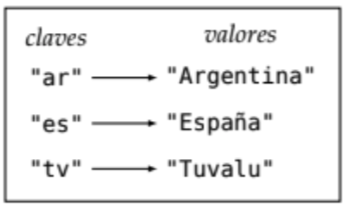
\includegraphics{./imgs/unidad_4/diccionarios1.png}

}

\caption{Diccionario cuyas claves son dominios de internet (.ar, .es,
.tv) y cuyos valores asociados son los países correspondientes.}

\end{figure}%

Las claves deben ser únicas, es decir, no puede haber dos claves iguales
en un mismo diccionario. Los valores pueden repetirse. Si se asigna un
valor a una clave ya existente, se reemplaza el valor anterior.

Podemos acceder a un valor a través de su clave porque las claves son
únicas, pero no a la inversa. Es decir, no podemos acceder a una clave a
través de su valor, porque los valores pueden repetirse y podría haber
varias claves asociadas al mismo valor.

Además, los diccionarios no tienen un orden interno particular. Se
consideran entonces iguales dos diccionarios si tienen las mismas claves
asociadas a los mismos valores, independientemente del orden en que se
hayan agregado.

Al igual que las listas, los diccionarios son mutables. Esto significa
que podemos modificar sus elementos una vez creados.

\begin{itemize}
\tightlist
\item
  Cualquier valor de tipo inmutable puede ser \texttt{clave} de un
  diccionario: cadenas, enteros tuplas.
\item
  No hay restricciones para los \texttt{valores}, pueden ser de
  cualquier tipo: cadenas, enteros, tuplas, listas, otros diccionarios,
  etc.
\end{itemize}

\subsection{Diccionarios en Python}\label{diccionarios-en-python}

Para definir un diccionario, se utilizan llaves \texttt{\{\}} y se
separan las claves de los valores con dos puntos \texttt{:}. Cada par
clave-valor se separa con comas \texttt{,}.

\begin{Shaded}
\begin{Highlighting}[]
\NormalTok{dominios }\OperatorTok{=}\NormalTok{ \{}\StringTok{"ar"}\NormalTok{: }\StringTok{"Argentina"}\NormalTok{, }\StringTok{"es"}\NormalTok{: }\StringTok{"España"}\NormalTok{, }\StringTok{"tv"}\NormalTok{: }\StringTok{"Tuvalu"}\NormalTok{\}}
\end{Highlighting}
\end{Shaded}

El tipo asociado a los diccionarios es \texttt{dict}:

\begin{Shaded}
\begin{Highlighting}[]
\BuiltInTok{print}\NormalTok{(}\BuiltInTok{type}\NormalTok{(dominios))}
\end{Highlighting}
\end{Shaded}

\begin{verbatim}
<class 'dict'>
\end{verbatim}

Para declararlo vacío y luego ingresar valores, se lo declara como un
par de llaves vacías. Luego, haciendo uso de la notación de corchetes
\texttt{{[}{]}}, se le asigna un valor a una clave:

\begin{Shaded}
\begin{Highlighting}[]
\NormalTok{materias }\OperatorTok{=}\NormalTok{ \{\}}
\NormalTok{materias[}\StringTok{"lunes"}\NormalTok{] }\OperatorTok{=}\NormalTok{ [}\DecValTok{6103}\NormalTok{, }\DecValTok{7540}\NormalTok{]}
\NormalTok{materias[}\StringTok{"martes"}\NormalTok{] }\OperatorTok{=}\NormalTok{ [}\DecValTok{6201}\NormalTok{]}
\NormalTok{materias[}\StringTok{"miércoles"}\NormalTok{] }\OperatorTok{=}\NormalTok{ [}\DecValTok{6103}\NormalTok{, }\DecValTok{7540}\NormalTok{]}
\NormalTok{materias[}\StringTok{"jueves"}\NormalTok{] }\OperatorTok{=}\NormalTok{ []}
\NormalTok{materias[}\StringTok{"viernes"}\NormalTok{] }\OperatorTok{=}\NormalTok{ [}\DecValTok{6201}\NormalTok{]}
\end{Highlighting}
\end{Shaded}

En el código de arriba, se está creando una variable \texttt{materias}
de tipo \texttt{dict}, y se le están asignando valores a las claves
\texttt{"lunes"}, \texttt{"martes"}, \texttt{"miércoles"},
\texttt{"jueves"} y \texttt{"viernes"}.\\
Los valores asociados a cada clave son listas con los códigos de las
materias que se dan esos días. El diccionario se ve algo así:

\begin{verbatim}
{
    "lunes": [6103, 7540],
    "martes": [6201],
    "miércoles": [6103, 7540],
    "jueves": [],
    "viernes": [6201]
}
\end{verbatim}

\subsection{Accediendo a los Valores de un
Diccionario}\label{accediendo-a-los-valores-de-un-diccionario}

Para acceder a los valores de un diccionario, se utiliza la notación de
corchetes \texttt{{[}{]}} con la clave correspondiente:

\begin{Shaded}
\begin{Highlighting}[]
\NormalTok{cods\_lunes }\OperatorTok{=}\NormalTok{ materias[}\StringTok{"lunes"}\NormalTok{]}
\BuiltInTok{print}\NormalTok{(cods\_lunes)}
\end{Highlighting}
\end{Shaded}

\begin{verbatim}
[6103, 7540]
\end{verbatim}

Veamos que la clave ``lunes'' no va a ser igual a la clave ``Lunes'' o
``LUNES'', porque como ya dijimos antes, Python es \emph{case
sensitive}.

\begin{tcolorbox}[enhanced jigsaw, bottomrule=.15mm, leftrule=.75mm, opacityback=0, colback=white, toprule=.15mm, bottomtitle=1mm, opacitybacktitle=0.6, rightrule=.15mm, left=2mm, arc=.35mm, coltitle=black, title=\textcolor{quarto-callout-warning-color}{\faExclamationTriangle}\hspace{0.5em}{¡Cuidado! Acceso a Claves que no Existen}, breakable, toptitle=1mm, colframe=quarto-callout-warning-color-frame, titlerule=0mm, colbacktitle=quarto-callout-warning-color!10!white]

Si intentamos acceder a una clave que no existe en el diccionario, se
produce un error:

\begin{Shaded}
\begin{Highlighting}[]
\BuiltInTok{print}\NormalTok{(materias[}\StringTok{"sábado"}\NormalTok{])}
\end{Highlighting}
\end{Shaded}

\begin{Shaded}
\begin{Highlighting}[]
\NormalTok{Traceback (most recent call last):}
\NormalTok{File "\textless{}stdin\textgreater{}", line 1, in \textless{}module\textgreater{}}
\NormalTok{KeyError: \textquotesingle{}sábado\textquotesingle{}}
\end{Highlighting}
\end{Shaded}

\end{tcolorbox}

\hfill\break
Para evitar tratar de acceder a una clave que no existe, podemos
verificar si una clave se encuentra o no en el diccionario haciendo uso
del operador \texttt{in}:

\begin{Shaded}
\begin{Highlighting}[]
\ControlFlowTok{if} \StringTok{"sábado"} \KeywordTok{in}\NormalTok{ materias:}
    \BuiltInTok{print}\NormalTok{(materias[}\StringTok{"sábado"}\NormalTok{])}
\ControlFlowTok{else}\NormalTok{:}
    \BuiltInTok{print}\NormalTok{(}\StringTok{"No hay clases el sábado"}\NormalTok{)}
\end{Highlighting}
\end{Shaded}

\begin{verbatim}
No hay clases el sábado
\end{verbatim}

También podemos usar la función \texttt{get}, que recibe una clave
\texttt{k}y un valor por omisión \texttt{v}, y devuelve el valor
asociado a la clave \texttt{k}, en caso de existir, o el valor
\texttt{v} en caso contrario.

\begin{Shaded}
\begin{Highlighting}[]
\BuiltInTok{print}\NormalTok{(materias.get(}\StringTok{"sábado"}\NormalTok{, }\StringTok{"Error de clave: sábado"}\NormalTok{))}
\end{Highlighting}
\end{Shaded}

\begin{verbatim}
Error de clave: sábado
\end{verbatim}

\begin{Shaded}
\begin{Highlighting}[]
\BuiltInTok{print}\NormalTok{(materias.get(}\StringTok{"domingo"}\NormalTok{,[]))}
\end{Highlighting}
\end{Shaded}

\begin{verbatim}
[]
\end{verbatim}

Como vemos el valor por omisión puede ser de cualquier tipo.

\subsection{Iterando Elementos del
Diccionario}\label{iterando-elementos-del-diccionario}

\subsubsection{Por Claves}\label{por-claves}

Para iterar sobre las claves de un diccionario, podemos usar un ciclo
\texttt{for}:

\begin{Shaded}
\begin{Highlighting}[]
\ControlFlowTok{for}\NormalTok{ dia }\KeywordTok{in}\NormalTok{ materias:}
    \BuiltInTok{print}\NormalTok{(}\SpecialStringTok{f"El }\SpecialCharTok{\{}\NormalTok{dia}\SpecialCharTok{\}}\SpecialStringTok{ tengo que cursar las materias }\SpecialCharTok{\{}\NormalTok{materias[dia]}\SpecialCharTok{\}}\SpecialStringTok{"}\NormalTok{)}
\end{Highlighting}
\end{Shaded}

\begin{verbatim}
El lunes tengo que cursar las materias [6103, 7540]
El martes tengo que cursar las materias [6201]
El miércoles tengo que cursar las materias [6103, 7540]
El jueves tengo que cursar las materias []
El viernes tengo que cursar las materias [6201]
\end{verbatim}

También podemos obtener las claves del diccionario como una lista usando
el método \texttt{keys()}:

\begin{Shaded}
\begin{Highlighting}[]
\ControlFlowTok{for}\NormalTok{ dia }\KeywordTok{in}\NormalTok{ materias.keys():}
    \BuiltInTok{print}\NormalTok{(}\SpecialStringTok{f"El }\SpecialCharTok{\{}\NormalTok{dia}\SpecialCharTok{\}}\SpecialStringTok{ tengo que cursar las materias }\SpecialCharTok{\{}\NormalTok{materias[dia]}\SpecialCharTok{\}}\SpecialStringTok{"}\NormalTok{)}
\end{Highlighting}
\end{Shaded}

\begin{verbatim}
El lunes tengo que cursar las materias [6103, 7540]
El martes tengo que cursar las materias [6201]
El miércoles tengo que cursar las materias [6103, 7540]
El jueves tengo que cursar las materias []
El viernes tengo que cursar las materias [6201]
\end{verbatim}

\subsubsection{Por Valores}\label{por-valores}

Para iterar sobre los valores de un diccionario, podemos usar el método
\texttt{values()}:

\begin{Shaded}
\begin{Highlighting}[]
\ControlFlowTok{for}\NormalTok{ codigos }\KeywordTok{in}\NormalTok{ materias.values():}
    \BuiltInTok{print}\NormalTok{(codigos)}
\end{Highlighting}
\end{Shaded}

\begin{verbatim}
[6103, 7540]
[6201]
[6103, 7540]
[]
[6201]
\end{verbatim}

Nótese que en este último ejemplo, no podemos obtener la clave a partir
de los valores. Por eso no imprimimos los \texttt{días}.

\subsubsection{Por Clave-Valor}\label{por-clave-valor}

Para iterar sobre los pares clave-valor de un diccionario, podemos usar
el método \texttt{items()}, que nos devuelve un conjunto de tuplas donde
el primer elemento de cada una es una clave y el segundo, su valor
asociado \texttt{(clave,valor)}:

\begin{Shaded}
\begin{Highlighting}[]
\ControlFlowTok{for}\NormalTok{ tupla }\KeywordTok{in}\NormalTok{ materias.items():}
\NormalTok{  dia }\OperatorTok{=}\NormalTok{ tupla[}\DecValTok{0}\NormalTok{]}
\NormalTok{  codigos }\OperatorTok{=}\NormalTok{ tupla[}\DecValTok{1}\NormalTok{]}
  \BuiltInTok{print}\NormalTok{(}\SpecialStringTok{f"El }\SpecialCharTok{\{}\NormalTok{dia}\SpecialCharTok{\}}\SpecialStringTok{ tengo que cursar las materias }\SpecialCharTok{\{}\NormalTok{codigos}\SpecialCharTok{\}}\SpecialStringTok{"}\NormalTok{)}
\end{Highlighting}
\end{Shaded}

\begin{verbatim}
El lunes tengo que cursar las materias [6103, 7540]
El martes tengo que cursar las materias [6201]
El miércoles tengo que cursar las materias [6103, 7540]
El jueves tengo que cursar las materias []
El viernes tengo que cursar las materias [6201]
\end{verbatim}

También podemos desempaquetar las tuplas como vimos previamente:

\begin{Shaded}
\begin{Highlighting}[]
\ControlFlowTok{for}\NormalTok{ dia, codigos }\KeywordTok{in}\NormalTok{ materias.items():}
  \BuiltInTok{print}\NormalTok{(}\SpecialStringTok{f"El }\SpecialCharTok{\{}\NormalTok{dia}\SpecialCharTok{\}}\SpecialStringTok{ tengo que cursar las materias }\SpecialCharTok{\{}\NormalTok{codigos}\SpecialCharTok{\}}\SpecialStringTok{"}\NormalTok{)}
\end{Highlighting}
\end{Shaded}

\begin{verbatim}
El lunes tengo que cursar las materias [6103, 7540]
El martes tengo que cursar las materias [6201]
El miércoles tengo que cursar las materias [6103, 7540]
El jueves tengo que cursar las materias []
El viernes tengo que cursar las materias [6201]
\end{verbatim}

\begin{tcolorbox}[enhanced jigsaw, bottomrule=.15mm, leftrule=.75mm, opacityback=0, colback=white, toprule=.15mm, bottomtitle=1mm, opacitybacktitle=0.6, rightrule=.15mm, left=2mm, arc=.35mm, coltitle=black, title=\textcolor{quarto-callout-note-color}{\faInfo}\hspace{0.5em}{Note}, breakable, toptitle=1mm, colframe=quarto-callout-note-color-frame, titlerule=0mm, colbacktitle=quarto-callout-note-color!10!white]

Como los diccionarios no son secuencias, no tienen orden interno
específico, por lo que no podemos obtener porciones de un diccionario
usando \emph{slices} o \texttt{{[}:{]}} como hacíamos con otras
estructuras de datos.

\end{tcolorbox}

\begin{tcolorbox}[enhanced jigsaw, bottomrule=.15mm, leftrule=.75mm, opacityback=0, colback=white, toprule=.15mm, bottomtitle=1mm, opacitybacktitle=0.6, rightrule=.15mm, left=2mm, arc=.35mm, coltitle=black, title=\textcolor{quarto-callout-tip-color}{\faLightbulb}\hspace{0.5em}{Acerca de la Iteración de un Diccionario}, breakable, toptitle=1mm, colframe=quarto-callout-tip-color-frame, titlerule=0mm, colbacktitle=quarto-callout-tip-color!10!white]

El mayor beneficio de los diccionarios es que podemos acceder a sus
valores de forma eficiente, a través de sus claves.\\
Si la única funcionalidad que necesitamos de un diccionario es iterarlo,
entonces no estamos aprovechando su potencial. En ese caso, es
preferible usar una o más listas o tuplas, que es más simple y más
eficiente.\\
Iterar un diccionario es una funcionalidad adicional que nos brinda
Python, pero no es su principal uso.

\end{tcolorbox}

\subsection{Usos de un Diccionario}\label{usos-de-un-diccionario}

Los diccionarios son muy versátiles. Se puede utilizar un diccionario
para, por ejemplo, contar cuántas apariciones de cada palabra hay en un
texto, o cuántas apariciones por cada letra.

También se puede usar un diccionario para tener una agenda de contactos,
donde la clave es el nombre de la persona y el valor el número de
teléfono.

\begin{tcolorbox}[enhanced jigsaw, bottomrule=.15mm, leftrule=.75mm, opacityback=0, colback=white, toprule=.15mm, bottomtitle=1mm, opacitybacktitle=0.6, rightrule=.15mm, left=2mm, arc=.35mm, coltitle=black, title=\textcolor{quarto-callout-note-color}{\faInfo}\hspace{0.5em}{Hashmaps: Dato interesante}, breakable, toptitle=1mm, colframe=quarto-callout-note-color-frame, titlerule=0mm, colbacktitle=quarto-callout-note-color!10!white]

Los diccionarios de Python son implementados usando una estructura de
datos llamada \emph{hashmap}.\\
Para cada clave, se le calcula un valor numérico llamado \emph{hash},
que es el que se usa para acceder al valor asociado a esa clave.\\
Cuando se recibe una clave, se le calcula su \emph{hash} y se busca en
el diccionario el valor asociado a ese \emph{hash}.\\

\end{tcolorbox}

\subsection{Operaciones de los
Diccionarios}\label{operaciones-de-los-diccionarios}

\begin{longtable}[]{@{}
  >{\raggedright\arraybackslash}p{(\columnwidth - 2\tabcolsep) * \real{0.5000}}
  >{\raggedright\arraybackslash}p{(\columnwidth - 2\tabcolsep) * \real{0.5000}}@{}}
\toprule\noalign{}
\begin{minipage}[b]{\linewidth}\raggedright
Operación
\end{minipage} & \begin{minipage}[b]{\linewidth}\raggedright
Descripción
\end{minipage} \\
\midrule\noalign{}
\endhead
\bottomrule\noalign{}
\endlastfoot
\texttt{d{[}k{]}} & Devuelve el valor asociado a la clave \texttt{k} \\
\texttt{d{[}k{]}\ =\ v} & Asigna el valor \texttt{v} a la clave
\texttt{k}. Si la clave no existe, la agrega al diccionario. Si ya
existe, le actualiza el valor asociado. \\
\texttt{del\ d{[}k{]}} & Elimina la clave \texttt{k} y su valor asociado
del diccionario \texttt{d} \\
\texttt{k\ in\ d} & Devuelve \texttt{True} si la clave \texttt{k} se
encuentra en el diccionario \texttt{d}, \texttt{False} en caso
contrario \\
\texttt{len(d)} & Devuelve la cantidad de pares clave-valor del
diccionario \texttt{d} \\
\texttt{d.keys()} & Devuelve una lista con las claves del diccionario
\texttt{d} \\
\texttt{d.values()} & Devuelve una lista con los valores del diccionario
\texttt{d} \\
\texttt{d.items()} & Devuelve una lista de tuplas con los pares
clave-valor del diccionario \texttt{d} \\
\texttt{d.clear()} & Elimina todos los pares clave-valor del diccionario
\texttt{d} \\
\texttt{d.copy()} & Devuelve una copia del diccionario \texttt{d} \\
\texttt{d.pop(k)} & Elimina la clave \texttt{k} y su valor asociado del
diccionario \texttt{d}, y devuelve el valor asociado \\
\texttt{d.popitem()} & Elimina un par clave-valor del diccionario
\texttt{d}, y devuelve una tupla con la clave y el valor eliminados \\
\texttt{d.get(k,\ v)} & Devuelve el valor asociado a la clave \texttt{k}
si la clave existe, o el valor \texttt{v} en caso contrario \\
\texttt{d.update(d2)} & Agrega los pares clave-valor del diccionario
\texttt{d2} al diccionario \texttt{d}. Si una clave ya existe en
\texttt{d}, actualiza su valor asociado. \\
\end{longtable}

\begin{tcolorbox}[enhanced jigsaw, bottomrule=.15mm, leftrule=.75mm, opacityback=0, colback=white, toprule=.15mm, bottomtitle=1mm, opacitybacktitle=0.6, rightrule=.15mm, left=2mm, arc=.35mm, coltitle=black, title=\textcolor{quarto-callout-note-color}{\faInfo}\hspace{0.5em}{Note}, breakable, toptitle=1mm, colframe=quarto-callout-note-color-frame, titlerule=0mm, colbacktitle=quarto-callout-note-color!10!white]

Existen más métodos de diccionarios, pero estos son los más utilizados y
los que vamos a ver en la materia. Recomendamos que pruebes cada uno de
ellos con los diccionarios que vimos en este capítulo.

\end{tcolorbox}

\subsection{Diccionarios y Funciones}\label{diccionarios-y-funciones}

Los diccionarios son mutables, por lo que podemos pasarlos como
parámetros a funciones y modificarlos dentro de la función.

\begin{Shaded}
\begin{Highlighting}[]
\KeywordTok{def}\NormalTok{ agregar\_alumno(alumnos, nombre, legajo):}
\NormalTok{  alumnos[nombre] }\OperatorTok{=}\NormalTok{ legajo}

\NormalTok{alumnos }\OperatorTok{=}\NormalTok{ \{\}}
\NormalTok{agregar\_alumno(alumnos, }\StringTok{"Juan"}\NormalTok{, }\DecValTok{1234}\NormalTok{)}
\NormalTok{agregar\_alumno(alumnos, }\StringTok{"María"}\NormalTok{, }\DecValTok{5678}\NormalTok{)}
\BuiltInTok{print}\NormalTok{(alumnos)}
\end{Highlighting}
\end{Shaded}

\begin{verbatim}
{'Juan': 1234, 'María': 5678}
\end{verbatim}

\subsection{Ordenamiento de
Diccionarios}\label{ordenamiento-de-diccionarios}

Tenemos algunas operaciones que nos permiten ordenar un diccionario:

\begin{longtable}[]{@{}
  >{\raggedright\arraybackslash}p{(\columnwidth - 2\tabcolsep) * \real{0.5000}}
  >{\raggedright\arraybackslash}p{(\columnwidth - 2\tabcolsep) * \real{0.5000}}@{}}
\toprule\noalign{}
\begin{minipage}[b]{\linewidth}\raggedright
Operación
\end{minipage} & \begin{minipage}[b]{\linewidth}\raggedright
Descripción
\end{minipage} \\
\midrule\noalign{}
\endhead
\bottomrule\noalign{}
\endlastfoot
\texttt{dict()} & Crea un diccionario vacío \\
\texttt{sorted(d)} & Devuelve una lista ordenada con las claves del
diccionario \texttt{d} \\
\texttt{dict(sorted(d.items()))} & Devuelve un diccionario ordenado con
las claves del diccionario \texttt{d} \\
\end{longtable}

Si lo que necesitamos es ordenar diccionarios entre sí (por ejemplo,
teniendo una lista de diccionarios), vamos a usar el parámetro
\texttt{key} de la función \texttt{sorted}:

\begin{Shaded}
\begin{Highlighting}[]
\KeywordTok{def}\NormalTok{ obtener\_nombre(alumno):}
  \ControlFlowTok{return}\NormalTok{ alumno[}\StringTok{"nombre"}\NormalTok{]}

\NormalTok{alumnos }\OperatorTok{=}\NormalTok{ [}
\NormalTok{  \{}\StringTok{"nombre"}\NormalTok{: }\StringTok{"Priscila"}\NormalTok{, }\StringTok{"legajo"}\NormalTok{: }\DecValTok{1234}\NormalTok{\},}
\NormalTok{  \{}\StringTok{"nombre"}\NormalTok{: }\StringTok{"Iara"}\NormalTok{, }\StringTok{"legajo"}\NormalTok{: }\DecValTok{5678}\NormalTok{\},}
\NormalTok{  \{}\StringTok{"nombre"}\NormalTok{: }\StringTok{"Agostina"}\NormalTok{, }\StringTok{"legajo"}\NormalTok{: }\DecValTok{9012}\NormalTok{\}}
\NormalTok{]}
\NormalTok{alumnos\_ordenados }\OperatorTok{=} \BuiltInTok{sorted}\NormalTok{(alumnos, key}\OperatorTok{=}\NormalTok{obtener\_nombre)}
\BuiltInTok{print}\NormalTok{(alumnos\_ordenados)}
\end{Highlighting}
\end{Shaded}

\begin{verbatim}
[{'nombre': 'Agostina', 'legajo': 9012}, {'nombre': 'Iara', 'legajo': 5678}, {'nombre': 'Priscila', 'legajo': 1234}]
\end{verbatim}

\begin{tcolorbox}[enhanced jigsaw, bottomrule=.15mm, leftrule=.75mm, opacityback=0, colback=white, toprule=.15mm, bottomtitle=1mm, opacitybacktitle=0.6, rightrule=.15mm, left=2mm, arc=.35mm, coltitle=black, title=\textcolor{quarto-callout-note-color}{\faInfo}\hspace{0.5em}{Note}, breakable, toptitle=1mm, colframe=quarto-callout-note-color-frame, titlerule=0mm, colbacktitle=quarto-callout-note-color!10!white]

En el ejemplo de arriba, estamos ordenando una lista de diccionarios por
el valor de la clave \texttt{"nombre"}.\\
El parámetro \texttt{key} recibe una función que se va a aplicar a cada
elemento de la lista antes de ordenar. En este caso, la función
\texttt{obtener\_nombre} devuelve el valor de la clave \texttt{"nombre"}
de cada diccionario, y es lo que se usa para ordenar.

\end{tcolorbox}

\begin{tcolorbox}[enhanced jigsaw, bottomrule=.15mm, leftrule=.75mm, opacityback=0, colback=white, toprule=.15mm, bottomtitle=1mm, opacitybacktitle=0.6, rightrule=.15mm, left=2mm, arc=.35mm, coltitle=black, title=\textcolor{quarto-callout-important-color}{\faExclamation}\hspace{0.5em}{Ejercicio Desafío}, breakable, toptitle=1mm, colframe=quarto-callout-important-color-frame, titlerule=0mm, colbacktitle=quarto-callout-important-color!10!white]

Escribir una función que reciba una lista de diccionarios y una clave, y
devuelva una lista con los diccionarios ordenados según la clave.\\

Ejemplo:\\
Si se tiene
\texttt{{[}\{"nombre":\ "Priscila",\ "legajo":\ 1234\},\ \{"nombre":\ "Iara",\ "legajo":\ 5678\},\ \{"nombre":\ "Agostina",\ "legajo":\ 9012\}{]}}
y se recibe la clave \texttt{nombre}\\
una vez ejecutada, la función debe devolver:\\
\texttt{{[}\{"nombre":\ "Agostina",\ "legajo":\ 9012\},\ \{"nombre":\ "Iara",\ "legajo":\ 5678\},\ \{"nombre":\ "Priscila",\ "legajo":\ 1234\}{]}}\strut \\

\end{tcolorbox}

\begin{tcolorbox}[enhanced jigsaw, bottomrule=.15mm, leftrule=.75mm, opacityback=0, colback=white, toprule=.15mm, bottomtitle=1mm, opacitybacktitle=0.6, rightrule=.15mm, left=2mm, arc=.35mm, coltitle=black, title=\textcolor{quarto-callout-tip-color}{\faLightbulb}\hspace{0.5em}{Lambda}, breakable, toptitle=1mm, colframe=quarto-callout-tip-color-frame, titlerule=0mm, colbacktitle=quarto-callout-tip-color!10!white]

En el ejemplo anterior, la función \texttt{obtener\_nombre} es muy
simple, y sólo la usamos una vez.\\
En estos casos, podemos usar una \emph{función lambda}, que es una
función anónima que se declara en una sola línea.\\

\begin{Shaded}
\begin{Highlighting}[]
\NormalTok{alumnos }\OperatorTok{=}\NormalTok{ [}
\NormalTok{  \{}\StringTok{"nombre"}\NormalTok{: }\StringTok{"Priscila"}\NormalTok{, }\StringTok{"legajo"}\NormalTok{: }\DecValTok{1234}\NormalTok{\},}
\NormalTok{  \{}\StringTok{"nombre"}\NormalTok{: }\StringTok{"Iara"}\NormalTok{, }\StringTok{"legajo"}\NormalTok{: }\DecValTok{5678}\NormalTok{\},}
\NormalTok{  \{}\StringTok{"nombre"}\NormalTok{: }\StringTok{"Agostina"}\NormalTok{, }\StringTok{"legajo"}\NormalTok{: }\DecValTok{9012}\NormalTok{\}}
\NormalTok{]}

\NormalTok{alumnos\_ordenados }\OperatorTok{=} \BuiltInTok{sorted}\NormalTok{(alumnos, key}\OperatorTok{=}\KeywordTok{lambda}\NormalTok{ alumno: alumno[}\StringTok{"nombre"}\NormalTok{])}
\BuiltInTok{print}\NormalTok{(alumnos\_ordenados)}
\end{Highlighting}
\end{Shaded}

\begin{verbatim}
[{'nombre': 'Agostina', 'legajo': 9012}, {'nombre': 'Iara', 'legajo': 5678}, {'nombre': 'Priscila', 'legajo': 1234}]
\end{verbatim}

Lo que estamos haciendo es declarar una función que recibe un parámetro
\texttt{alumno} y devuelve el valor de la clave \texttt{"nombre"} de ese
diccionario.\\
La función se declara en una sola línea, y no tiene nombre.\\
La función se pasa como parámetro \texttt{key} a \texttt{sorted}, y se
ejecuta para cada elemento de la lista antes de ordenar.

\end{tcolorbox}

\section{Sets}\label{sets}

Un set es una estructura de datos mutable (como las listas y los
diccionarios), que permite agregar y quitar elementos cumpliendo los
requisitos de unicidad y búsqueda en tiempo constante. Además, es
posible hacer operaciones entre sets como la unión, intersección y
diferencia.

La sintaxis de un set es con llaves \texttt{\{\}}, al igual que el
diccionario, pero no contiene pares de clave-valor asociados, únicamente
elementos.

\begin{Shaded}
\begin{Highlighting}[]
\NormalTok{s1 }\OperatorTok{=}\NormalTok{ \{}\DecValTok{1}\NormalTok{, }\DecValTok{2}\NormalTok{, }\DecValTok{3}\NormalTok{, }\DecValTok{4}\NormalTok{\}}
\BuiltInTok{print}\NormalTok{(s1)}
\end{Highlighting}
\end{Shaded}

\begin{verbatim}
{1, 2, 3, 4}
\end{verbatim}

El set no permite tener elementos repetidos, por lo que tratar de
agregar un elemento a un set en donde ya existe, no lo agrega por
duplicado:

\begin{Shaded}
\begin{Highlighting}[]
\NormalTok{s1.add(}\DecValTok{1}\NormalTok{)}
\BuiltInTok{print}\NormalTok{(s1)}
\end{Highlighting}
\end{Shaded}

\begin{verbatim}
{1, 2, 3, 4}
\end{verbatim}

Para unir dos sets, podemos usar el método \texttt{union}:

\begin{Shaded}
\begin{Highlighting}[]
\NormalTok{s2 }\OperatorTok{=}\NormalTok{ \{}\DecValTok{3}\NormalTok{,}\DecValTok{4}\NormalTok{,}\DecValTok{5}\NormalTok{,}\DecValTok{6}\NormalTok{\}}
\NormalTok{s1.union(s2)}
\BuiltInTok{print}\NormalTok{(s1)}
\end{Highlighting}
\end{Shaded}

\begin{verbatim}
{1, 2, 3, 4}
\end{verbatim}

También podemos ver la intersección, y la diferencia:

\begin{Shaded}
\begin{Highlighting}[]
\NormalTok{intersection }\OperatorTok{=}\NormalTok{ s1.intersection(s2)}
\NormalTok{diff }\OperatorTok{=}\NormalTok{ s1.difference(s2)}

\BuiltInTok{print}\NormalTok{(}\SpecialStringTok{f"La intersección de s1 y s2 es }\SpecialCharTok{\{}\NormalTok{intersection}\SpecialCharTok{\}}\SpecialStringTok{ y la diferencia es: }\SpecialCharTok{\{}\NormalTok{diff}\SpecialCharTok{\}}\SpecialStringTok{"}\NormalTok{)}
\end{Highlighting}
\end{Shaded}

\begin{verbatim}
La intersección de s1 y s2 es {3, 4} y la diferencia es: {1, 2}
\end{verbatim}

Para crear un set vacío, no podemos usar un par de llaves \texttt{\{\}},
porque esa es sintaxis para crear un diccionario vacío. Lo que tenemos
que hacer es usar el método \texttt{set()}.

\begin{Shaded}
\begin{Highlighting}[]
\NormalTok{legajos }\OperatorTok{=} \BuiltInTok{set}\NormalTok{()}

\NormalTok{legajos.add(}\DecValTok{105609}\NormalTok{)}
\BuiltInTok{print}\NormalTok{(legajos)}
\end{Highlighting}
\end{Shaded}

\begin{verbatim}
{105609}
\end{verbatim}

\subsection{Operaciones con Sets}\label{operaciones-con-sets}

\begin{longtable}[]{@{}
  >{\raggedright\arraybackslash}p{(\columnwidth - 2\tabcolsep) * \real{0.5000}}
  >{\raggedright\arraybackslash}p{(\columnwidth - 2\tabcolsep) * \real{0.5000}}@{}}
\toprule\noalign{}
\begin{minipage}[b]{\linewidth}\raggedright
Operación
\end{minipage} & \begin{minipage}[b]{\linewidth}\raggedright
Descripción
\end{minipage} \\
\midrule\noalign{}
\endhead
\bottomrule\noalign{}
\endlastfoot
\texttt{s.add(x)} & Agrega el elemento \texttt{x} al set \texttt{s} \\
\texttt{s.remove(x)} & Elimina el elemento \texttt{x} del set
\texttt{s}. Si \texttt{x} no se encuentra en \texttt{s}, se produce un
error \\
\texttt{s.discard(x)} & Elimina el elemento \texttt{x} del set
\texttt{s}. Si \texttt{x} no se encuentra en \texttt{s}, no se produce
un error \\
\texttt{s.clear()} & Elimina todos los elementos del set \texttt{s} \\
\texttt{s.copy()} & Devuelve una copia del set \texttt{s} \\
\texttt{s.union(s2)} & Devuelve un set con los elementos de \texttt{s} y
\texttt{s2} \\
\texttt{s.intersection(s2)} & Devuelve un set con los elementos que
están en \texttt{s} y en \texttt{s2} \\
\texttt{s.difference(s2)} & Devuelve un set con los elementos que están
en \texttt{s} pero no en \texttt{s2} \\
len(s) & Devuelve la cantidad de elementos en \texttt{s} \\
x in s & Devuelve True si el elemento \texttt{x} se encuentra en
\texttt{s} \\
\end{longtable}

\subsection{Ordenamiento e Iteración de
Sets}\label{ordenamiento-e-iteraciuxf3n-de-sets}

Un set es un conjunto de datos sin ordenar. Sin embargo, podemos de
todas formas y si quisiéramos, ordenar los elementos haciendo uso de
\texttt{sorted}. El método \texttt{sort()} no está disponible para los
sets.

\begin{Shaded}
\begin{Highlighting}[]
\NormalTok{s3 }\OperatorTok{=}\NormalTok{ \{}\DecValTok{1}\NormalTok{,}\DecValTok{7}\NormalTok{,}\DecValTok{2}\NormalTok{,}\DecValTok{8}\NormalTok{,}\DecValTok{4}\NormalTok{\}}
\BuiltInTok{print}\NormalTok{(}\BuiltInTok{sorted}\NormalTok{(s3))}
\end{Highlighting}
\end{Shaded}

\begin{verbatim}
[1, 2, 4, 7, 8]
\end{verbatim}

Los elementos también pueden iterarse:

\begin{Shaded}
\begin{Highlighting}[]
\NormalTok{s4 }\OperatorTok{=}\NormalTok{ \{}\DecValTok{1}\NormalTok{, }\DecValTok{2}\NormalTok{, }\DecValTok{3}\NormalTok{, }\DecValTok{4}\NormalTok{\}}
\ControlFlowTok{for}\NormalTok{ e }\KeywordTok{in}\NormalTok{ s4:}
  \BuiltInTok{print}\NormalTok{(e)}
\end{Highlighting}
\end{Shaded}

\begin{verbatim}
1
2
3
4
\end{verbatim}

\bookmarksetup{startatroot}

\chapter{Entrada y Salida}\label{entrada-y-salida}

\section{Archivos}\label{archivos}

Cuando un programa se esta ejecutando los datos están en la memoria,
pero cuando el programa termina los datos se pierden.

Para almacenar los datos de forma permanente se hace uso de
\textbf{archivos}. Cada archivo se identifica con un nombre unico dentro
de directorio o carpeta en que se encuentre. Por ejemplo dentro la
carpeta \emph{Documentos} puede existir solo un archivo con el nombre
\emph{Apuntes.txt}.

Los archivos se utilizan para organizar los datos e intercambiarlos para
distintos fines. El modo de trabajar con archivos es como trabajar con
libros, se pueden abrir, leer, escribir y cerrar. Además se puede leer
en orden o secuencialmente o yendo a un lugar especifico.

\begin{tcolorbox}[enhanced jigsaw, bottomrule=.15mm, leftrule=.75mm, opacityback=0, colback=white, toprule=.15mm, bottomtitle=1mm, opacitybacktitle=0.6, rightrule=.15mm, left=2mm, arc=.35mm, coltitle=black, title=\textcolor{quarto-callout-note-color}{\faInfo}\hspace{0.5em}{Note}, breakable, toptitle=1mm, colframe=quarto-callout-note-color-frame, titlerule=0mm, colbacktitle=quarto-callout-note-color!10!white]

Toda la organización de las computadoras esta basada en archivos y
directorios.

\end{tcolorbox}

\subsection{Abriendo un Archivo}\label{abriendo-un-archivo}

En python para abrir un archivo utilizamos la función \texttt{open}

\begin{Shaded}
\begin{Highlighting}[]
\NormalTok{ruta\_archivo }\OperatorTok{=} \StringTok{"alumnos.txt"}
\NormalTok{archivo }\OperatorTok{=} \BuiltInTok{open}\NormalTok{(ruta\_archivo)}
\end{Highlighting}
\end{Shaded}

Esta función intentara abrir el archivo ``alumnos.txt'' y si tiene éxito
en la variable archivo quedara un tipo de dato que nos permitira
manipularlo.

\subsection{Leyendo un Archivo}\label{leyendo-un-archivo}

La operación más frecuente con los archivos es leerlos de forma
secuencial

\begin{Shaded}
\begin{Highlighting}[]
\NormalTok{archivo }\OperatorTok{=} \BuiltInTok{open}\NormalTok{(ruta\_archivo)}
\NormalTok{linea }\OperatorTok{=}\NormalTok{ archivo.readline()}

\ControlFlowTok{while}\NormalTok{ linea }\OperatorTok{!=} \StringTok{\textquotesingle{}\textquotesingle{}}\NormalTok{:}
  \CommentTok{\# hacer algo con la linea}
\NormalTok{  linea }\OperatorTok{=}\NormalTok{ archivo.readline()}

\NormalTok{archivo.close()}
\end{Highlighting}
\end{Shaded}

Este último bloque de código lee todas las lineas (renglones) del
archivo hasta que no queden más.

La variable \texttt{archivo}, que mencionamos más arriba como un ``tipo
de dato que nos permitira manipularlo'' guarda cual es la siguiente
posición que debe leer y cuando se ejecuta \texttt{archivo.readline()}
lee esa posición y avanza una posición más.

La función \texttt{close()} cierra el archivo, esta operación es
importante para mantener la consistencia de la información. Volveremos
más adelante sobre este tema.

\begin{quote}
\textbf{Ejemplo} ``alumnos.txt''
\end{quote}

\begin{Shaded}
\begin{Highlighting}[]
\NormalTok{DNI;Nombre;Nota}
\NormalTok{45000001;Mariana Szischik;9}
\NormalTok{46000001;Emilia Duzac;8}
\NormalTok{46000001;Lucia Capon;9}
\end{Highlighting}
\end{Shaded}

En el ejemplo anterior leimos el archivo linea por linea, pero existe
otra forma de leer un archivo. Veamos otro ejemplo.

\begin{Shaded}
\begin{Highlighting}[]
\NormalTok{archivo }\OperatorTok{=} \BuiltInTok{open}\NormalTok{(ruta\_archivo)}
\NormalTok{lineas }\OperatorTok{=}\NormalTok{ archivo.readlines()}
\NormalTok{archivo.close()}

\ControlFlowTok{for}\NormalTok{ linea }\KeywordTok{in}\NormalTok{ lineas:}
  \CommentTok{\# hacer algo con la linea}
  \BuiltInTok{print}\NormalTok{(linea)}
\end{Highlighting}
\end{Shaded}

\begin{Shaded}
\begin{Highlighting}[]
\ExtensionTok{linea}\NormalTok{ número 0 }
\ExtensionTok{linea}\NormalTok{ número 1 }
\ExtensionTok{linea}\NormalTok{ número 2 }
\ExtensionTok{linea}\NormalTok{ número 3 }
\ExtensionTok{linea}\NormalTok{ número 4 }
\end{Highlighting}
\end{Shaded}

\textbf{¿ Que diferencias hay entre el ejemplo de más arriba y éste ?}

La diferencia pricipal y que condiciona el resto de los cambios es que
en lugar de leer linea por linea utilizamos la funcion
\texttt{readlines()}. Esta función leer \emph{todo} el contenido del
archivo y devueve una lista donde cada elemento de la lista es un
renglón. Por otro lado se llama a la función \texttt{close()}
inmediatamente después de leer todo el archivo. ¿ Por qué ? ¿ Te animas
a analizar todas las diferencias ?

\subsubsection{Resumen}\label{resumen}

\begin{itemize}
\tightlist
\item
  \texttt{read()}: Lee todo el archivo y lo devuelve como una cadena de
  texto.
\item
  \texttt{readline()}: Lee una línea del archivo y la devuelve como una
  cadena de texto. Cuando se llega al final del archivo, devuelve una
  cadena vacía.
\item
  \texttt{readlines()}: Lee todas las líneas del archivo y las devuelve
  como una lista de cadenas de texto.
\end{itemize}

\subsection{Escribiendo en un archivo}\label{escribiendo-en-un-archivo}

Python también tiene métodos para escribir archivos, los más comunes
son:

\begin{itemize}
\tightlist
\item
  \texttt{write()}: Escribe una cadena de texto en el archivo.
\item
  \texttt{writelines()}: Escribe una lista de cadenas de texto en el
  archivo.
\end{itemize}

\begin{Shaded}
\begin{Highlighting}[]
\NormalTok{ruta\_archivo\_nuevo }\OperatorTok{=} \StringTok{"saludo.txt"}
\NormalTok{archivo }\OperatorTok{=} \BuiltInTok{open}\NormalTok{(ruta\_archivo\_nuevo, }\StringTok{\textquotesingle{}w\textquotesingle{}}\NormalTok{)}

\NormalTok{archivo.write(}\StringTok{"Hola!}\CharTok{\textbackslash{}n}\StringTok{"}\NormalTok{)}
\NormalTok{archivo.writelines([}\StringTok{"¿Cómo estás?}\CharTok{\textbackslash{}n}\StringTok{"}\NormalTok{, }\StringTok{"Espero que bien.}\CharTok{\textbackslash{}n}\StringTok{"}\NormalTok{])}
\NormalTok{archivo.close()}
\end{Highlighting}
\end{Shaded}

\begin{tcolorbox}[enhanced jigsaw, bottomrule=.15mm, leftrule=.75mm, opacityback=0, colback=white, toprule=.15mm, bottomtitle=1mm, opacitybacktitle=0.6, rightrule=.15mm, left=2mm, arc=.35mm, coltitle=black, title=\textcolor{quarto-callout-tip-color}{\faLightbulb}\hspace{0.5em}{Tip}, breakable, toptitle=1mm, colframe=quarto-callout-tip-color-frame, titlerule=0mm, colbacktitle=quarto-callout-tip-color!10!white]

En este ejemplo se puede ver el uso de \texttt{\textbackslash{}n}. Este
caracter es lo que indica a los medios de salida de información que lo
que se escribió finaliza con una nueva linea. Ninguno de los métodos de
escritura agrega automáticamente un salto de línea al final de lo que se
escribe, a menos que se lo indiquemos explícitamente.

Cuando leemos un archivo tenemos que tener en cuenta que el último
caracter de cada linea va a ser \texttt{\textbackslash{}n}

\end{tcolorbox}

Pero no todos los archivos pueden ser escritos, por ejemplo los archivos
que se encuentran en modo lectura (`r'). ¿De qué depende? Depende del
tipo de acceso con el que se abrió el archivo.

\subsection{Tipos de acceso}\label{tipos-de-acceso}

Cuando se abre un archivo hay que especificar para qué lo estamos
abriendo, las opciones en general son: leer o escribir. Por defecto, si
no especificamos nada, tal como vimos en los ejemplos anteriores, se
abre para leer.

\begin{figure}[H]

{\centering 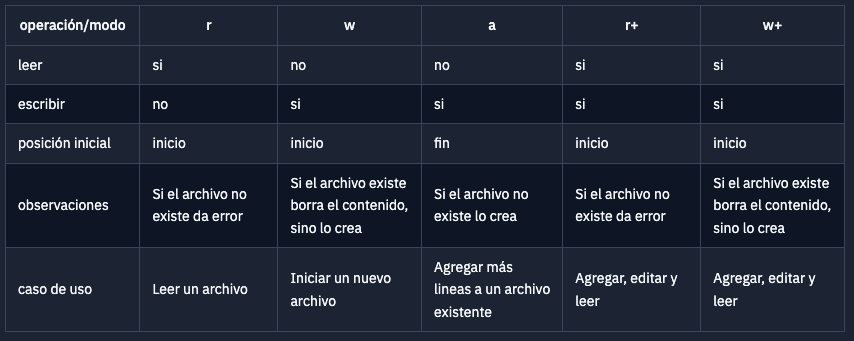
\includegraphics{./imgs/unidad_5/tipos_acceso.png}

}

\caption{Resumen de los tipos de acceso con los que se puede abrir un
archivo.}

\end{figure}%

Veamos ejemplos de los casos más comunes

\begin{quote}
\textbf{Ejemplo Write (w)}
\end{quote}

\begin{Shaded}
\begin{Highlighting}[]
\NormalTok{ruta\_archivo\_nuevo }\OperatorTok{=} \StringTok{"alumnos\_nuevo.txt"}
\NormalTok{archivo }\OperatorTok{=} \BuiltInTok{open}\NormalTok{(ruta\_archivo\_nuevo, }\StringTok{\textquotesingle{}w\textquotesingle{}}\NormalTok{)}

\ControlFlowTok{for}\NormalTok{ x }\KeywordTok{in} \BuiltInTok{range}\NormalTok{(}\DecValTok{5}\NormalTok{):}
  \CommentTok{\# hacer algo con la linea}
\NormalTok{  archivo.write(}\SpecialStringTok{f"linea número }\SpecialCharTok{\{}\NormalTok{x}\SpecialCharTok{\}}\SpecialStringTok{ }\CharTok{\textbackslash{}n}\SpecialStringTok{"}\NormalTok{)}

\NormalTok{archivo.close()}
\end{Highlighting}
\end{Shaded}

\begin{quote}
\textbf{Ejemplo Read (r)}
\end{quote}

\begin{Shaded}
\begin{Highlighting}[]
\NormalTok{archivo }\OperatorTok{=} \BuiltInTok{open}\NormalTok{(ruta\_archivo\_nuevo, }\StringTok{\textquotesingle{}r\textquotesingle{}}\NormalTok{)}
\NormalTok{lineas }\OperatorTok{=}\NormalTok{ archivo.readlines()}
\NormalTok{archivo.close()}

\ControlFlowTok{for}\NormalTok{ linea }\KeywordTok{in}\NormalTok{ lineas:}
  \CommentTok{\# hacer algo con la linea}
  \BuiltInTok{print}\NormalTok{(linea)}
\end{Highlighting}
\end{Shaded}

\begin{quote}
\textbf{Ejemplo Append (a)}
\end{quote}

\begin{Shaded}
\begin{Highlighting}[]
\NormalTok{archivo }\OperatorTok{=} \BuiltInTok{open}\NormalTok{(ruta\_archivo\_nuevo, }\StringTok{\textquotesingle{}a\textquotesingle{}}\NormalTok{)}
\NormalTok{archivo.write(}\StringTok{"linea número 5 }\CharTok{\textbackslash{}n}\StringTok{"}\NormalTok{) }\CommentTok{\# agrega una nueva linea al final del archivo}
\NormalTok{archivo.close()}
\end{Highlighting}
\end{Shaded}

\subsection{Close}\label{close}

Al terminar de trabajar con un archivo, es importante cerrarlo, por
diversos motivos: en algunos sistemas los archivos sólo pueden ser
abiertos de a un programa por la vez; en otros, lo que se haya escrito
no se guardará realmente hasta no cerrar el archivo.

\begin{Shaded}
\begin{Highlighting}[]
\NormalTok{archivo }\OperatorTok{=} \BuiltInTok{open}\NormalTok{(ruta\_archivo)}
\NormalTok{lineas }\OperatorTok{=}\NormalTok{ archivo.readlines()}
\NormalTok{archivo.close()}
\end{Highlighting}
\end{Shaded}

\begin{tcolorbox}[enhanced jigsaw, bottomrule=.15mm, leftrule=.75mm, opacityback=0, colback=white, toprule=.15mm, bottomtitle=1mm, opacitybacktitle=0.6, rightrule=.15mm, left=2mm, arc=.35mm, coltitle=black, title=\textcolor{quarto-callout-warning-color}{\faExclamationTriangle}\hspace{0.5em}{Warning}, breakable, toptitle=1mm, colframe=quarto-callout-warning-color-frame, titlerule=0mm, colbacktitle=quarto-callout-warning-color!10!white]

Cuando abrimos un archivo, queremos dejarlo abierto siempre la
\textbf{menor cantidad de tiempo posible}. Si abrimos un archivo y no lo
cerramos, estamos ocupando recursos del sistema que podrían ser
utilizados por otros programas. Por lo que tenemos que pensar muy bien
la forma de armar nuestro código para que los archivos se abran y
cierren sólo cuando los necesitamos usar.

\end{tcolorbox}

Una forma de asegurarse de que un archivo se cierre es utilizar la
sentencia \texttt{with}. Esta sentencia se encarga de cerrar el archivo
automáticamente al finalizar el bloque de código que se le pasa.

\begin{Shaded}
\begin{Highlighting}[]
\ControlFlowTok{with} \BuiltInTok{open}\NormalTok{(ruta\_archivo) }\ImportTok{as}\NormalTok{ archivo:}
\NormalTok{  lineas }\OperatorTok{=}\NormalTok{ archivo.readlines()}

\CommentTok{\# Acá el archivo ya se cerró sólo}
\end{Highlighting}
\end{Shaded}

\begin{tcolorbox}[enhanced jigsaw, bottomrule=.15mm, leftrule=.75mm, opacityback=0, colback=white, toprule=.15mm, bottomtitle=1mm, opacitybacktitle=0.6, rightrule=.15mm, left=2mm, arc=.35mm, coltitle=black, title=\textcolor{quarto-callout-tip-color}{\faLightbulb}\hspace{0.5em}{Tip}, breakable, toptitle=1mm, colframe=quarto-callout-tip-color-frame, titlerule=0mm, colbacktitle=quarto-callout-tip-color!10!white]

¿ Te animas a probar que pasa si intentas escribir en un archivo que fue
abierto para lectura (`r') y a leer en uno que fue abierto para
escritura (`w') ?

\end{tcolorbox}

\subsection{Ejemplos}\label{ejemplos-1}

Veamos un ejemplo en el que trabajaremos con dos archivos.

\begin{quote}
\textbf{Ejemplo} Obtener un el promedio de notas y guardarlo en un nuevo
archivo llamado ``promedio.txt''
\end{quote}

\begin{Shaded}
\begin{Highlighting}[]
\CommentTok{\# Abrimos el archivo de notas}
\NormalTok{ruta\_archivo }\OperatorTok{=} \StringTok{"alumnos.txt"}
\NormalTok{archivo }\OperatorTok{=} \BuiltInTok{open}\NormalTok{(ruta\_archivo, }\StringTok{\textquotesingle{}r\textquotesingle{}}\NormalTok{)}
\NormalTok{lineas }\OperatorTok{=}\NormalTok{ archivo.readlines()}
\NormalTok{archivo.close()}

\CommentTok{\# Leemos linea por linea cada nota }
\NormalTok{suma\_notas }\OperatorTok{=} \DecValTok{0}
\NormalTok{cantidad\_notas }\OperatorTok{=} \DecValTok{0}
\ControlFlowTok{for}\NormalTok{ linea }\KeywordTok{in}\NormalTok{ lineas[}\DecValTok{1}\NormalTok{:]: }\CommentTok{\# la primer línea no contiene datos, solo los nombres de los campos}
\NormalTok{  nota }\OperatorTok{=}\NormalTok{ linea.split(}\StringTok{";"}\NormalTok{)[}\DecValTok{2}\NormalTok{].strip(}\StringTok{\textquotesingle{}}\CharTok{\textbackslash{}n}\StringTok{\textquotesingle{}}\NormalTok{) }\CommentTok{\# nos quedamos con la nota}
\NormalTok{  suma\_notas }\OperatorTok{+=} \BuiltInTok{int}\NormalTok{(nota)}
\NormalTok{  cantidad\_notas }\OperatorTok{+=} \DecValTok{1}

\CommentTok{\# Guardamos el promedio en un nuevo archivo}
\NormalTok{ruta\_archivo\_promedios }\OperatorTok{=} \StringTok{"promedio.txt"}
\NormalTok{archivo }\OperatorTok{=} \BuiltInTok{open}\NormalTok{(ruta\_archivo\_promedios, }\StringTok{\textquotesingle{}w\textquotesingle{}}\NormalTok{)}
\NormalTok{archivo.write(}\BuiltInTok{str}\NormalTok{(suma\_notas}\OperatorTok{/}\NormalTok{cantidad\_notas))}
\NormalTok{archivo.close()}
\end{Highlighting}
\end{Shaded}

Veamos el contenido del archivo ``promedio.txt''

\begin{Shaded}
\begin{Highlighting}[]
\NormalTok{ruta\_archivo }\OperatorTok{=} \StringTok{"promedio.txt"}
\NormalTok{archivo }\OperatorTok{=} \BuiltInTok{open}\NormalTok{(ruta\_archivo, }\StringTok{\textquotesingle{}r\textquotesingle{}}\NormalTok{)}
\NormalTok{linea }\OperatorTok{=}\NormalTok{ archivo.readline()}
\NormalTok{archivo.close()}
\BuiltInTok{print}\NormalTok{(linea)}
\end{Highlighting}
\end{Shaded}

\begin{Shaded}
\begin{Highlighting}[]
\ExtensionTok{6.25}
\end{Highlighting}
\end{Shaded}

En el ejemplo anterior hay al menos dos cosas que vale la pena remarcar:
el uso de la función \texttt{split()}\footnote{\href{https://docs.python.org/es/3/library/stdtypes.html\#str.split}{Split}}
nos permite separar cada linea en una lista que tiene 3 elementos, a
nosostros nos interesa el elemento que esta en la posición 2, la nota;
por otro lado también utilizamos la función \texttt{strip()}\footnote{\href{https://docs.python.org/es/3/library/stdtypes.html\#str.strip}{Strip}},
esto remueve el caracter de nueva linea \texttt{\textbackslash{}n} y nos
permite leer la nota como un número.

Un detalle que no hay que evadir cómo se recorre la lista teniendo en
cuenta que la primer linea del archivo no nos interesa ya que contiene
los nombres de cada campo. Esto se explica en
\hyperref[listas-como-secuencias]{unidad 4}.

\subsection{Tipos de archivos}\label{tipos-de-archivos}

En la sección anterior utilizamos para todos los archivos la extención
`.txt' el uso de extenciónes es una \textbf{convención}, una manera de
nombrar las cosas que nos da una idea de lo que hay en el contenido del
archivo.

Comunmente a los archivos que estuvimos usando como ejemplo se los
nombra con la extención `.csv' las siglas de ``comma separated
values''\footnote{\href{https://es.wikipedia.org/wiki/Valores_separados_por_comas}{CSV}}.

\subsection{Conclusiones}\label{conclusiones}

\begin{itemize}
\tightlist
\item
  Para utilizar un archivo desde un programa, es necesario abrirlo, y
  cuando ya no se lo necesite, se lo debe cerrar.
\item
  Las instrucciones más básicas para manejar un archivo son leer y
  escribir.
\item
  Los archivos de texto se procesan generalmente línea por línea y
  sirven para intercambiar información entre diversos programas o entre
  programas y humanos.
\end{itemize}

\section{Manejo de errores}\label{manejo-de-errores}

Cuando cometemos un error de tipeo o utilizamos mal una sentencia el
interprete nos muestra un error de sintaxis. En la practica lo vemos
como un \texttt{SintaxisError}, este tipo de errores se los llama
errores sintácticos, la menera de resolverlo es revisar la sintáxis y
corregirlo.

\textbf{Ejemplo: Función mal definida}

\begin{Shaded}
\begin{Highlighting}[]
\NormalTok{deff incrementar(n):}
  \ControlFlowTok{return}\NormalTok{ n }\OperatorTok{+} \DecValTok{1}
\end{Highlighting}
\end{Shaded}

\begin{verbatim}
 File ...., line 1
    deff incrementar(n):
         ^^^^^^^^^^^
SyntaxError: invalid syntax
\end{verbatim}

Cuando un programa se esta ejecutando y ocurre un error se crea una
excepción, normalmente el programa detiene su ejecución y se imprime un
mensaje. Este tipo de errores se los llama \textbf{errores de
ejecución}, vamos a ver como manejarlos.

\textbf{Ejemplo: División por cero}

\begin{Shaded}
\begin{Highlighting}[]
\NormalTok{dividendo }\OperatorTok{=} \DecValTok{10}
\NormalTok{divisor }\OperatorTok{=} \DecValTok{0}
\NormalTok{resultado }\OperatorTok{=}\NormalTok{ dividendo}\OperatorTok{/}\NormalTok{divisor }
\end{Highlighting}
\end{Shaded}

\begin{Shaded}
\begin{Highlighting}[]
\ExtensionTok{{-}{-}{-}{-}{-}{-}{-}{-}{-}{-}{-}{-}{-}{-}{-}{-}{-}{-}{-}{-}{-}{-}{-}{-}{-}{-}{-}{-}{-}{-}{-}{-}{-}{-}{-}{-}{-}{-}{-}{-}{-}{-}{-}{-}{-}{-}{-}{-}{-}{-}{-}{-}{-}{-}{-}{-}{-}{-}{-}{-}{-}{-}{-}{-}{-}{-}{-}{-}{-}{-}{-}{-}{-}{-}{-}}
\ExtensionTok{ZeroDivisionError}\NormalTok{                         Traceback }\ErrorTok{(}\ExtensionTok{most}\NormalTok{ recent call last}\KeywordTok{)}
\ExtensionTok{File}\NormalTok{ ...}
      \ExtensionTok{1}\NormalTok{ dividendo = 10}
      \ExtensionTok{2}\NormalTok{ divisor = 0}
\ExtensionTok{{-}{-}{-}{-}}\OperatorTok{\textgreater{}}\NormalTok{ 3 resultado = dividendo/divisor }
\ExtensionTok{ZeroDivisionError:}\NormalTok{ division by zero}
\end{Highlighting}
\end{Shaded}

\textbf{Ejemplo: Acceso a un elemento que no existe}

\begin{Shaded}
\begin{Highlighting}[]
\NormalTok{lista }\OperatorTok{=}\NormalTok{ [}\StringTok{"a"}\NormalTok{,}\StringTok{"b"}\NormalTok{]}
\NormalTok{segundo\_elemento }\OperatorTok{=}\NormalTok{ lista[}\DecValTok{2}\NormalTok{]}
\end{Highlighting}
\end{Shaded}

\begin{Shaded}
\begin{Highlighting}[]
\ExtensionTok{{-}{-}{-}{-}{-}{-}{-}{-}{-}{-}{-}{-}{-}{-}{-}{-}{-}{-}{-}{-}{-}{-}{-}{-}{-}{-}{-}{-}{-}{-}{-}{-}{-}{-}{-}{-}{-}{-}{-}{-}{-}{-}{-}{-}{-}{-}{-}{-}{-}{-}{-}{-}{-}{-}{-}{-}{-}{-}{-}{-}{-}{-}{-}{-}{-}{-}{-}{-}{-}{-}{-}{-}{-}{-}{-}}
\ExtensionTok{IndexError}\NormalTok{                                Traceback }\ErrorTok{(}\ExtensionTok{most}\NormalTok{ recent call last}\KeywordTok{)}
\ExtensionTok{File}\NormalTok{ /...}
      \ExtensionTok{1}\NormalTok{ lista = }\PreprocessorTok{[}\StringTok{"a"}\SpecialStringTok{,}\StringTok{"b"}\PreprocessorTok{]}
\ExtensionTok{{-}{-}{-}{-}}\OperatorTok{\textgreater{}}\NormalTok{ 2 segundo\_elemento = lista}\PreprocessorTok{[}\SpecialStringTok{2}\PreprocessorTok{]}
\ExtensionTok{IndexError:}\NormalTok{ list index out of range}
\end{Highlighting}
\end{Shaded}

\textbf{Ejemplo: Abrir un archivo que no existe}

\begin{Shaded}
\begin{Highlighting}[]
\NormalTok{archivo }\OperatorTok{=} \BuiltInTok{open}\NormalTok{(}\StringTok{"archivo\_falso.txt"}\NormalTok{,}\StringTok{"r"}\NormalTok{)}
\end{Highlighting}
\end{Shaded}

\begin{Shaded}
\begin{Highlighting}[]
\ExtensionTok{FileNotFoundError}\NormalTok{                         Traceback }\ErrorTok{(}\ExtensionTok{most}\NormalTok{ recent call last}\KeywordTok{)}
\ExtensionTok{File}\NormalTok{ ...}
\ExtensionTok{{-}{-}{-}{-}}\OperatorTok{\textgreater{}}\NormalTok{ 1 archivo = open}\ErrorTok{(}\StringTok{"archivo\_falso.txt"}\ExtensionTok{,}\StringTok{"r"}\KeywordTok{)}
\ExtensionTok{FileNotFoundError:}\NormalTok{ [Errno 2] No such file or directory: }\StringTok{\textquotesingle{}archivo\_falso.txt\textquotesingle{}}
\end{Highlighting}
\end{Shaded}

En cada caso el mensaje de error tiene dos partes, la primera indica el
tipo de error:

\begin{itemize}
\tightlist
\item
  \texttt{ZeroDivisionError}
\item
  \texttt{IndexError}
\item
  \texttt{FileNotFoundError}
\end{itemize}

La segunda tiene una descripción:

\begin{itemize}
\tightlist
\item
  \texttt{division\ by\ zero}
\item
  \texttt{list\ index\ out\ of\ range}
\item
  \texttt{No\ such\ file\ or\ directory}
\end{itemize}

Además nos da información contextual que puede indicar en la ejecucuión
de qué linea se dió el error:

\begin{itemize}
\tightlist
\item
  Linea 3:
  \texttt{-\/-\/-\/-\textgreater{}\ 3\ resultado\ =\ dividendo/divisor}.
\item
  Linea 2:
  \texttt{-\/-\/-\/-\textgreater{}\ 2\ segundo\_elemento\ =\ lista{[}2{]}}.
\item
  Linea 1:
  \texttt{-\/-\/-\/-\textgreater{}\ 1\ archivo\ =\ open("archivo\_falso.txt","r")}.
\end{itemize}

En algunas ocaciones es parte del programa manejar operaciones que
puedan lanzar este tipo de excepciones sin que el programa detenga su
ejecución, para estos casos Python nos provee las sentencias
\texttt{try}y \texttt{except}.

\textbf{Ejemplo}

\begin{Shaded}
\begin{Highlighting}[]
\NormalTok{dividendo }\OperatorTok{=} \DecValTok{10}
\NormalTok{divisor }\OperatorTok{=} \DecValTok{0}
\ControlFlowTok{try}\NormalTok{:}
\NormalTok{  resultado }\OperatorTok{=}\NormalTok{ dividendo}\OperatorTok{/}\NormalTok{divisor }
\ControlFlowTok{except} \PreprocessorTok{ZeroDivisionError}\NormalTok{:}
  \BuiltInTok{print}\NormalTok{(}\StringTok{"No se puede dividir por cero."}\NormalTok{)}
\end{Highlighting}
\end{Shaded}

\begin{Shaded}
\begin{Highlighting}[]
\ExtensionTok{No}\NormalTok{ se puede dividir por cero.}
\end{Highlighting}
\end{Shaded}

Como se ve en el ejemplo se ``envuelve'' la operación que puede generar
ese tipo de excepción para que lo que resulte de esa operación se pueda
controlar. Como vimos más arriba hay distintos tipos de excepciones, la
lista completa se puede ver en
\href{https://docs.python.org/es/3/library/exceptions.html\#base-classes}{excepciones}.

\subsection{Validaciones}\label{validaciones}

Las validaciones son técnicas que permiten asegurar que los valores con
los que se vaya a operar estén dentro de determinado conjunto de
posibilidades o que tengan ciertas características.

Si bien quien invoca una función debe preocuparse de cumplir con las
precondiciones de ésta, si las validaciones están hechas correctamente
pueden devolver información valiosa para que el invocante pueda actuar
en consecuencia.

También se debe tener en cuenta qué hará nuestro código cuando una
validación falle, ya que queremos darle información al invocante que le
sirva para procesar el error. El error producido tiene que ser
fácilmente reconocible.

Ejemplo:

\begin{Shaded}
\begin{Highlighting}[]
\KeywordTok{def}\NormalTok{ convertir\_a\_int(ingreso\_usuario):}
  \ControlFlowTok{try}\NormalTok{:}
    \ControlFlowTok{return} \BuiltInTok{int}\NormalTok{(ingreso\_usuario)}
  \ControlFlowTok{except} \PreprocessorTok{ValueError}\NormalTok{:}
    \BuiltInTok{print}\NormalTok{(}\StringTok{"El valor ingresado no es un número"}\NormalTok{)}

\NormalTok{convertir\_a\_int(}\StringTok{"cuarenta"}\NormalTok{)}
\end{Highlighting}
\end{Shaded}

\begin{verbatim}
El valor ingresado no es un número
\end{verbatim}

\begin{tcolorbox}[enhanced jigsaw, bottomrule=.15mm, leftrule=.75mm, opacityback=0, colback=white, toprule=.15mm, bottomtitle=1mm, opacitybacktitle=0.6, rightrule=.15mm, left=2mm, arc=.35mm, coltitle=black, title=\textcolor{quarto-callout-note-color}{\faInfo}\hspace{0.5em}{Note}, breakable, toptitle=1mm, colframe=quarto-callout-note-color-frame, titlerule=0mm, colbacktitle=quarto-callout-note-color!10!white]

En Python también tenemos una forma de \emph{arrojar} nosotros un error,
es decir, hacer que la función falle y devuelva un mensaje de error.
Esto se hace con la sentencia \texttt{raise}. No lo vemos en la materia,
pero se usaría de la siguiente manera:

\begin{Shaded}
\begin{Highlighting}[]
\KeywordTok{def}\NormalTok{ dividir(n1, n2):}
  \ControlFlowTok{if}\NormalTok{ n2 }\OperatorTok{==} \DecValTok{0}\NormalTok{:}
    \ControlFlowTok{raise} \PreprocessorTok{ZeroDivisionError}\NormalTok{(}\StringTok{"No se puede dividir por cero"}\NormalTok{)}
  \ControlFlowTok{return}\NormalTok{ n1}\OperatorTok{/}\NormalTok{n2}

\NormalTok{dividir(}\DecValTok{10}\NormalTok{, }\DecValTok{0}\NormalTok{)}
\end{Highlighting}
\end{Shaded}

\begin{verbatim}
ZeroDivisionError: No se puede dividir por cero
\end{verbatim}

Arrojar o levantar excepciones es un tema complejo, porque además de
arrojarlas, debemos ser capaces de capturarlas y manejarlas. Es por esto
que no se incluye en el temario de la materia.

\end{tcolorbox}

\subsection{Conclusiones}\label{conclusiones-1}

\begin{itemize}
\tightlist
\item
  El manejo de errores es un parte fundamental en el desarrollo de
  software, tan importante como la funcionalidad que se está
  programando.
\item
  Los errores que se dan en tiempo de ejecución los podemos ``atrapar''
  con el bloque \texttt{try}.
\item
  Hay tipos de excepciones que describen distintos tipos de errores de
  ejecución.
\end{itemize}

\subsection{Bonus Track: Tipos de
Errores}\label{bonus-track-tipos-de-errores}

A continuación se presenta una tabla con los errores más comunes que se
pueden encontrar al programar en Python.

\begin{longtable}[]{@{}
  >{\raggedright\arraybackslash}p{(\columnwidth - 4\tabcolsep) * \real{0.3333}}
  >{\raggedright\arraybackslash}p{(\columnwidth - 4\tabcolsep) * \real{0.3333}}
  >{\raggedright\arraybackslash}p{(\columnwidth - 4\tabcolsep) * \real{0.3333}}@{}}
\toprule\noalign{}
\begin{minipage}[b]{\linewidth}\raggedright
Tipo de error
\end{minipage} & \begin{minipage}[b]{\linewidth}\raggedright
Descripción
\end{minipage} & \begin{minipage}[b]{\linewidth}\raggedright
Más Información
\end{minipage} \\
\midrule\noalign{}
\endhead
\bottomrule\noalign{}
\endlastfoot
SyntaxError & Error de sintaxis & Suele ser un error de tipeo o de uso
incorrecto de una sentencia \\
ZeroDivisionError & División por cero & Se produce cuando se intenta
dividir por cero \\
NameError & Variable no definida & Se produce cuando se intenta utilizar
una variable que no fue definida \\
IndexError & Índice fuera de rango & Se produce cuando se intenta
acceder a un elemento de una secuencia, que no existe \\
FileNotFoundError & Archivo no encontrado & Se produce cuando se intenta
abrir un archivo que no existe \\
TypeError & Tipo de dato incorrecto & Se produce cuando se intenta
realizar una operación con un tipo de dato incorrecto \\
ValueError & Valor incorrecto & Se produce cuando se intenta realizar
una operación con un valor incorrecto \\
KeyError & Clave no encontrada & Se produce cuando se intenta acceder a
un elemento de un diccionario que no existe \\
IOError & Error de entrada/salida & Se produce cuando se intenta
realizar una operación de entrada/salida que no se puede realizar (por
ejemplo, intentar acceder a un archivo) \\
\end{longtable}

\bookmarksetup{startatroot}

\chapter{Bibliotecas de Python}\label{bibliotecas-de-python}

\section{Introducción}\label{introducciuxf3n-1}

Python es un lenguaje de programación muy popular, poderoso y versátil
que cuenta con una amplia gama de bibliotecas que ayudan a que la
programación sea más fácil y eficiente. Pero, \textbf{¿qué son las
bibliotecas?} La bibliotecas son conjuntos de módulos que contienen
funciones, clases y variables relacionadas, que permiten realizar tareas
sin tener que escribir el código desde cero y este se puede reutilizar
en múltiples programas y proyectos.

Entre las bibliotecas disponibles se encuentran las estándares, que se
incluye con cada instalación de Python, y las de código abierto creadas
por la gran comunidad de desarrolladores, que constantemente genera
nuevas bibliotecas y mejora las existentes. Por ello es aconsejable que,
al momento de utilizarlas, se verifique si existe alguna actualización
en las guías de usuario.

Asimismo, estas bibliotecas se pueden clasificar según su aplicación y
funcionalidad en: procesamiento de datos, visualización, aprendizaje
automático, desarrollo web, procesamiento de lenguaje y de imágenes,
entre otras. En este capítulo se analizarán tres de las bibliotecas más
reconocidas y ampliamente utilizadas de Python: \textbf{NumPy} y
\textbf{Pandas} para procesamiento de datos y \textbf{Matplotlib}, para
visualización.

\subsection{¿Cómo se utilizan las
bibliotecas?}\label{cuxf3mo-se-utilizan-las-bibliotecas}

Para acceder a una biblioteca y sus funciones, se debe instalar por
única vez y luego, importar cada vez que la necesitemos.

En la parte superior de nuestro código debemos correr
\texttt{import\ \{nombre\_de\_biblioteca\}\ as\ \{nombre\_corto\_de\_biblioteca\}}.
El alias o nombre corto de la biblioteca se suele agregar para lograr
una mayor legilibilidad del código, pero no es mandatorio.

\begin{Shaded}
\begin{Highlighting}[]
\ImportTok{import}\NormalTok{ numpy }\ImportTok{as}\NormalTok{ np}
\end{Highlighting}
\end{Shaded}

\begin{tcolorbox}[enhanced jigsaw, bottomrule=.15mm, leftrule=.75mm, opacityback=0, colback=white, toprule=.15mm, bottomtitle=1mm, opacitybacktitle=0.6, rightrule=.15mm, left=2mm, arc=.35mm, coltitle=black, title=\textcolor{quarto-callout-note-color}{\faInfo}\hspace{0.5em}{Note}, breakable, toptitle=1mm, colframe=quarto-callout-note-color-frame, titlerule=0mm, colbacktitle=quarto-callout-note-color!10!white]

En nuestro caso, la instalación no es necesaria ya que vamos a utilizar
Google Colab o Replit, pero en caso de usar otro IDE (como por ejemplo,
Visual Studio Code), se realiza desde el símbolo del sistema (o en
inglés: ``Command Prompt'', o terminal o consola), corriendo:
\texttt{pip\ install\ –nombre\_de\_biblioteca}.

\end{tcolorbox}

\section{NumPy}\label{numpy}

NumPy es una biblioteca de código abierto muy utilizada en el campo de
la ciencia y la ingeniería. Permite trabajar con datos numéricos,
matrices multidimensionales, funciones matemáticas y estadísticas
avanzadas.

Como ya se mencionó anteriormente, para utilizarse se debe instalar e
importar. Por convención, se suele importar como:

\begin{Shaded}
\begin{Highlighting}[]
\ImportTok{import}\NormalTok{ numpy }\ImportTok{as}\NormalTok{ np}
\end{Highlighting}
\end{Shaded}

NumPy incorpora una estructura de datos propia llamados \textbf{arrays}
que es similar a la lista de Python, pero puede almacenar y operar con
datos de manera mucho más eficiente: \textbf{el procesamiento de los
arrays es hasta 50 veces más rápido}. Esta diferencia de velocidad se
debe, en parte, a que \textbf{los arrays contienen datos homogéneos}, a
diferencia de las listas que pueden contener distintos tipos de datos
dentro.

\subsection{\texorpdfstring{\textbf{Arrays}}{Arrays}}\label{arrays}

Un \textbf{array} es un conjunto de elementos del mismo tipo, donde cada
uno de ellos posee una posición y esta es única para cada elemento. Como
dijimos arriba, en Python vimos las listas, que es lo más parecido a un
Array.

Analicemos el siguiente ejemplo: si pensamos en una matriz, lo primero
que nos viene a la mente es una tabla con valores ordenados en filas y
columnas, donde una fila es la línea horizontal y una columna es la
vertical. Es decir, una matriz es un conjunto de elementos que posee una
posición o índice determinado determinado por la fila y la columna, por
lo que sería un array.

En este capítulo se trabajará principalmente con vectores y matrices ya
que consideramos que les será útil para aplicar los conocimientos de
Numpy en otras materias.

\subsubsection{Creación de un Array}\label{creaciuxf3n-de-un-array}

Un array se crea usando la función \texttt{array()} a partir de listas o
tuplas. Por ejemplo:

\begin{Shaded}
\begin{Highlighting}[]
\NormalTok{a }\OperatorTok{=}\NormalTok{ np.array([}\DecValTok{1}\NormalTok{, }\DecValTok{2}\NormalTok{, }\DecValTok{3}\NormalTok{])}
\BuiltInTok{print}\NormalTok{(a)}
\end{Highlighting}
\end{Shaded}

\begin{verbatim}
[1 2 3]
\end{verbatim}

También, se pueden crear arrays particulares, constituídos por ceros con
\texttt{zeros()} o por unos con \texttt{ones()}:

\begin{Shaded}
\begin{Highlighting}[]
\CommentTok{\# Creo un array de ceros con dos elementos}
\NormalTok{a\_ceros }\OperatorTok{=}\NormalTok{ np.zeros(}\DecValTok{2}\NormalTok{)}
\BuiltInTok{print}\NormalTok{(a\_ceros)}
\end{Highlighting}
\end{Shaded}

\begin{verbatim}
[0. 0.]
\end{verbatim}

\begin{Shaded}
\begin{Highlighting}[]
\CommentTok{\# Creo un array de unos con dos elementos}
\NormalTok{a\_unos }\OperatorTok{=}\NormalTok{ np.ones(}\DecValTok{2}\NormalTok{)}
\BuiltInTok{print}\NormalTok{(a\_unos)}
\end{Highlighting}
\end{Shaded}

\begin{verbatim}
[1. 1.]
\end{verbatim}

Además, se pueden crear arrays con un rango de números, utilizando
\texttt{arange()} o \texttt{linspace()}:

\begin{Shaded}
\begin{Highlighting}[]
\CommentTok{\# Creo un array con un rango que empieza en 2 hasta 9 y va de 2 en 2.}
\NormalTok{a\_rango }\OperatorTok{=}\NormalTok{ np.arange(}\DecValTok{2}\NormalTok{, }\DecValTok{9}\NormalTok{, }\DecValTok{2}\NormalTok{)}
\BuiltInTok{print}\NormalTok{(a\_rango)}
\end{Highlighting}
\end{Shaded}

\begin{verbatim}
[2 4 6 8]
\end{verbatim}

\begin{Shaded}
\begin{Highlighting}[]
\CommentTok{\# Creo un array con un rango formado por 4 números}
\CommentTok{\# que empieza en 2 hasta 10 (incluídos). }
\NormalTok{a\_rango\_2 }\OperatorTok{=}\NormalTok{ np.linspace(}\DecValTok{2}\NormalTok{, }\DecValTok{10}\NormalTok{, num}\OperatorTok{=}\DecValTok{4}\NormalTok{)}
\BuiltInTok{print}\NormalTok{(a\_rango\_2)}
\end{Highlighting}
\end{Shaded}

\begin{verbatim}
[ 2.          4.66666667  7.33333333 10.        ]
\end{verbatim}

Esto es muy parecido a los rangos que ya vimos en Python, con la sutil
diferencia de que el \texttt{final} del rango en este caso \textbf{sí se
icnluye}.

Finalmente, para crear arrays de más dimensiones, se utilizan varias
listas:

\begin{Shaded}
\begin{Highlighting}[]
\NormalTok{matriz }\OperatorTok{=}\NormalTok{ np.array([[}\DecValTok{1}\NormalTok{, }\DecValTok{2}\NormalTok{, }\DecValTok{3}\NormalTok{], [}\DecValTok{4}\NormalTok{, }\DecValTok{5}\NormalTok{, }\DecValTok{6}\NormalTok{]])}

\BuiltInTok{print}\NormalTok{(matriz)}
\end{Highlighting}
\end{Shaded}

\begin{verbatim}
[[1 2 3]
 [4 5 6]]
\end{verbatim}

\subsubsection{Atributos de un array}\label{atributos-de-un-array}

\subsubsection{Dimensión}\label{dimensiuxf3n}

Para caracterizar un array es necesario conocer sus dimensiones,
utilizando \texttt{ndim}. De esta forma, se puede confirmar que el array
llamado \textbf{matriz}, definido anteriormente, es bidimensional:

\begin{Shaded}
\begin{Highlighting}[]
\CommentTok{\# Número de ejes o dimensiones de la matriz}
\NormalTok{matriz.ndim}
\end{Highlighting}
\end{Shaded}

\begin{verbatim}
2
\end{verbatim}

\subsubsection{Forma}\label{forma}

Otra característica de interés es su forma o \texttt{shape}: para las
matrices bidimensionales, se muestra una tupla (n, m) con el número de
filas n y de columnas m:

\begin{Shaded}
\begin{Highlighting}[]
\CommentTok{\# (n = filas, m = columnas)}
\NormalTok{matriz.shape}
\end{Highlighting}
\end{Shaded}

\begin{verbatim}
(2, 3)
\end{verbatim}

\subsubsection{Tamaño}\label{tamauxf1o}

El tamaño de un array es el número total de elementos que contiene, y se
obtiene con \texttt{size}:

\begin{Shaded}
\begin{Highlighting}[]
\CommentTok{\# Número total de elementos de la matriz: 2 filas x 3 columnas = 6 elementos}
\NormalTok{matriz.size}
\end{Highlighting}
\end{Shaded}

\begin{verbatim}
6
\end{verbatim}

\subsubsection{Posiciones}\label{posiciones}

Al elemento de una matriz A que se encuentra en la \textbf{fila i-ésima
y la columna j-ésima} se llama \(a_{ij}\). Así, para acceder a un
elemento de un array se debe indicar primero la posición de la fila y
luego, de la columna:

\begin{Shaded}
\begin{Highlighting}[]
\BuiltInTok{print}\NormalTok{(}\StringTok{\textquotesingle{}Elemento de la primera fila y segunda columna: \textquotesingle{}}\NormalTok{, matriz[}\DecValTok{0}\NormalTok{, }\DecValTok{1}\NormalTok{])}
\end{Highlighting}
\end{Shaded}

\begin{verbatim}
Elemento de la primera fila y segunda columna:  2
\end{verbatim}

Nótese la diferencia con las matrices (listas de listas) de Python,
donde se accedía a un elemento por separado, primero a la fila y luego a
la columna: \texttt{matriz{[}0{]}{[}1{]}}.

También se puede elegir un rango de elementos en una fila o columna
particular:

\begin{Shaded}
\begin{Highlighting}[]
\BuiltInTok{print}\NormalTok{(}\StringTok{\textquotesingle{}Los elementos de la primera fila, columnas 0 y 1: \textquotesingle{}}\NormalTok{, matriz[}\DecValTok{0}\NormalTok{, }\DecValTok{0}\NormalTok{:}\DecValTok{2}\NormalTok{])}
\end{Highlighting}
\end{Shaded}

\begin{verbatim}
Los elementos de la primera fila, columnas 0 y 1:  [1 2]
\end{verbatim}

\begin{Shaded}
\begin{Highlighting}[]
\BuiltInTok{print}\NormalTok{(}\StringTok{\textquotesingle{}Los elementos de la segunda columna, filas 0 y 1: \textquotesingle{}}\NormalTok{, matriz[}\DecValTok{0}\NormalTok{:}\DecValTok{2}\NormalTok{, }\DecValTok{1}\NormalTok{])}
\end{Highlighting}
\end{Shaded}

\begin{verbatim}
Los elementos de la segunda columna, filas 0 y 1:  [2 5]
\end{verbatim}

\subsubsection{Modificar arrays}\label{modificar-arrays}

De forma similar a lo aprendido con las listas de Python, se pueden
modificar los arrays utilizando ciertas funciones. Para entender y
aplicar las mismas, definamos un vector llamado a:

\begin{Shaded}
\begin{Highlighting}[]
\NormalTok{a }\OperatorTok{=}\NormalTok{ np.array([}\DecValTok{2}\NormalTok{, }\DecValTok{1}\NormalTok{, }\DecValTok{5}\NormalTok{, }\DecValTok{3}\NormalTok{, }\DecValTok{7}\NormalTok{, }\DecValTok{4}\NormalTok{, }\DecValTok{6}\NormalTok{, }\DecValTok{8}\NormalTok{])}

\BuiltInTok{print}\NormalTok{(a)}
\end{Highlighting}
\end{Shaded}

\begin{verbatim}
[2 1 5 3 7 4 6 8]
\end{verbatim}

\paragraph{Reshape}\label{reshape}

A este vector, se le puede modificar la forma: pasando de ser
\texttt{(8,)} a \texttt{(4,2)}, por dar un ejemplo:

\begin{Shaded}
\begin{Highlighting}[]
\NormalTok{a\_reshape }\OperatorTok{=}\NormalTok{ a.reshape(}\DecValTok{2}\NormalTok{, }\DecValTok{4}\NormalTok{) }\CommentTok{\# 2 filas y 4 columnas}

\BuiltInTok{print}\NormalTok{(a\_reshape)}
\end{Highlighting}
\end{Shaded}

\begin{verbatim}
[[2 1 5 3]
 [7 4 6 8]]
\end{verbatim}

\paragraph{Insert}\label{insert}

También, se modría insertar una fila (\texttt{axis\ =\ 0}) o una columna
(\texttt{axis\ =\ 1}) en una determinada posición. Por ejemplo:

\begin{Shaded}
\begin{Highlighting}[]
\CommentTok{\# Agregar fila de cincos en posición 1:}
\BuiltInTok{print}\NormalTok{(np.insert(a\_reshape, }\DecValTok{1}\NormalTok{, }\DecValTok{5}\NormalTok{, axis}\OperatorTok{=}\DecValTok{0}\NormalTok{))}
\end{Highlighting}
\end{Shaded}

\begin{verbatim}
[[2 1 5 3]
 [5 5 5 5]
 [7 4 6 8]]
\end{verbatim}

A la función \texttt{insert()}, se le debe indicar:\\

\begin{itemize}
\tightlist
\item
  El array que se desea modificar\\
\item
  La posición de la fila o columna que se desea agregar\\
\item
  Los valores a insertar. \textbf{¡Ojo con las dimensiones!} Para el
  ejemplo anterior, a\_reshape tenía 2 filas, por lo que se debe agregar
  una columna con 2 elementos o una fila con 4.\\
\item
  El eje que se agrega: una fila (axis = 0) o una columna (axis = 1)\\
\end{itemize}

\begin{Shaded}
\begin{Highlighting}[]
\CommentTok{\# Agregar columna de cincos en posición 1:}
\BuiltInTok{print}\NormalTok{(np.insert(a\_reshape, }\DecValTok{1}\NormalTok{, }\DecValTok{5}\NormalTok{, axis}\OperatorTok{=}\DecValTok{1}\NormalTok{))}
\end{Highlighting}
\end{Shaded}

\begin{verbatim}
[[2 5 1 5 3]
 [7 5 4 6 8]]
\end{verbatim}

O lo que es equivalente:

\begin{Shaded}
\begin{Highlighting}[]
\CommentTok{\# Agregar columna de cincos en posición 1:}
\BuiltInTok{print}\NormalTok{(np.insert(a\_reshape, }\DecValTok{1}\NormalTok{, [}\DecValTok{5}\NormalTok{, }\DecValTok{5}\NormalTok{], axis}\OperatorTok{=}\DecValTok{1}\NormalTok{))}
\end{Highlighting}
\end{Shaded}

\begin{verbatim}
[[2 5 1 5 3]
 [7 5 4 6 8]]
\end{verbatim}

\paragraph{Append y Delete}\label{append-y-delete}

También podríamos agregar una fila o una columna utilizando
\texttt{append()} al final, como ocurría con las listas:

\begin{Shaded}
\begin{Highlighting}[]
\CommentTok{\# Agregar una última fila}
\NormalTok{a\_modificada }\OperatorTok{=}\NormalTok{ np.append(a\_reshape, [[}\DecValTok{1}\NormalTok{, }\DecValTok{2}\NormalTok{, }\DecValTok{3}\NormalTok{, }\DecValTok{4}\NormalTok{]], axis}\OperatorTok{=}\DecValTok{0}\NormalTok{)}
\BuiltInTok{print}\NormalTok{(a\_modificada)}
\end{Highlighting}
\end{Shaded}

\begin{verbatim}
[[2 1 5 3]
 [7 4 6 8]
 [1 2 3 4]]
\end{verbatim}

O eliminarlas con \texttt{delete()}

\begin{Shaded}
\begin{Highlighting}[]
\CommentTok{\# Eliminar la fila de la posición 2.}
\BuiltInTok{print}\NormalTok{(np.delete(a\_modificada, }\DecValTok{2}\NormalTok{, axis}\OperatorTok{=}\DecValTok{0}\NormalTok{))}
\end{Highlighting}
\end{Shaded}

\begin{verbatim}
[[2 1 5 3]
 [7 4 6 8]]
\end{verbatim}

\paragraph{Concatenate y Sort}\label{concatenate-y-sort}

Finalmente, podemos concatenar arrays, como los siguientes:

\begin{Shaded}
\begin{Highlighting}[]
\NormalTok{a }\OperatorTok{=}\NormalTok{ np.array([}\DecValTok{2}\NormalTok{, }\DecValTok{1}\NormalTok{, }\DecValTok{5}\NormalTok{, }\DecValTok{3}\NormalTok{])}
\NormalTok{b }\OperatorTok{=}\NormalTok{ np.array([}\DecValTok{7}\NormalTok{, }\DecValTok{4}\NormalTok{, }\DecValTok{6}\NormalTok{, }\DecValTok{8}\NormalTok{])}

\CommentTok{\# Concatenar a y b:}
\NormalTok{c }\OperatorTok{=}\NormalTok{ np.concatenate((a, b))}
\BuiltInTok{print}\NormalTok{(c)}
\end{Highlighting}
\end{Shaded}

\begin{verbatim}
[2 1 5 3 7 4 6 8]
\end{verbatim}

Y ordenar los elementos de un array como numérico o alfabético,
ascendente o descendente.

\begin{Shaded}
\begin{Highlighting}[]
\BuiltInTok{print}\NormalTok{(np.sort(c))}
\end{Highlighting}
\end{Shaded}

\begin{verbatim}
[1 2 3 4 5 6 7 8]
\end{verbatim}

\subsection{\texorpdfstring{Operaciones aritméticas utilizando
\textbf{array}}{Operaciones aritméticas utilizando array}}\label{operaciones-aritmuxe9ticas-utilizando-array}

Como se ha mencionado anteriormente, Numpy tiene un gran potencial para
realizar operaciones, muy superior al de las listas de Python. Por
ejemplo, si quisieramos sumar dos listas de python necesitaríamos
realizar un \texttt{for}:

\begin{Shaded}
\begin{Highlighting}[]
\CommentTok{\# Definir listas}
\NormalTok{a }\OperatorTok{=}\NormalTok{ [}\DecValTok{2}\NormalTok{, }\DecValTok{1}\NormalTok{, }\DecValTok{5}\NormalTok{, }\DecValTok{3}\NormalTok{]}
\NormalTok{b }\OperatorTok{=}\NormalTok{ [}\DecValTok{7}\NormalTok{, }\DecValTok{4}\NormalTok{, }\DecValTok{6}\NormalTok{, }\DecValTok{8}\NormalTok{]}
\NormalTok{c }\OperatorTok{=}\NormalTok{ []}

\CommentTok{\# Sumar el primer elemento de a con el primero de b, el segundo elemento de a con el segundo de b y así sucesivamente}
\ControlFlowTok{for}\NormalTok{ i }\KeywordTok{in} \BuiltInTok{range}\NormalTok{(}\BuiltInTok{len}\NormalTok{(a)):}
\NormalTok{  c.append(a[i] }\OperatorTok{+}\NormalTok{ b[i])}
\BuiltInTok{print}\NormalTok{(c)}
\end{Highlighting}
\end{Shaded}

\begin{verbatim}
[9, 5, 11, 11]
\end{verbatim}

Utlizando las funciones de Numpy, esto ya no es más necesario:

\begin{Shaded}
\begin{Highlighting}[]
\CommentTok{\# add() para sumar elemento a elemento de a y b}
\NormalTok{c }\OperatorTok{=}\NormalTok{ np.add(a, b)}
\BuiltInTok{print}\NormalTok{(c)}
\end{Highlighting}
\end{Shaded}

\begin{verbatim}
[ 9  5 11 11]
\end{verbatim}

También podemos realizar otras operaciones, como la resta,
multiplicación y división. Usar un arreglo dentro de una ecuación nos
devuelve otro arreglo, donde cada elemento es el resultado de aplicar la
operación a los elementos correspondientes de los arreglos originales.

\begin{Shaded}
\begin{Highlighting}[]
\NormalTok{x }\OperatorTok{=}\NormalTok{ np.array([}\DecValTok{0}\NormalTok{,  }\DecValTok{1}\NormalTok{, }\DecValTok{2}\NormalTok{, }\DecValTok{3}\NormalTok{, }\DecValTok{4}\NormalTok{, }\DecValTok{5}\NormalTok{, }\DecValTok{6}\NormalTok{, }\DecValTok{7}\NormalTok{, }\DecValTok{8}\NormalTok{, }\DecValTok{9}\NormalTok{, }\DecValTok{10}\NormalTok{])}
\NormalTok{y }\OperatorTok{=} \DecValTok{3} \OperatorTok{*}\NormalTok{ x }\OperatorTok{+} \DecValTok{2}
\BuiltInTok{print}\NormalTok{(y)}
\end{Highlighting}
\end{Shaded}

\begin{verbatim}
[ 2  5  8 11 14 17 20 23 26 29 32]
\end{verbatim}

De esta forma, podemos realizar operaciones aritméticas con arrays de
Numpy de forma muy sencilla y rápida. Antes, en Python, para realizar
estas operaciones debíamos recurrir a un ciclo \texttt{for} o a el uso
de \texttt{map}. Numpy se ocupa de ahorrarnos el trabajo y calcular,
para cada elemento del array, el resultado.

Además, tenemos operaciones básicas que vienen predefinidas por Numpy.
Las vamos a ver a continuación.

\subsubsection{Operaciones básicas:}\label{operaciones-buxe1sicas}

A continuación se muestra una lista con las operaciones básicas junto
con sus operadores asociados, funciones y ejemplos.

\begin{longtable}[]{@{}lll@{}}
\toprule\noalign{}
Operación & Operador & Función \\
\midrule\noalign{}
\endhead
\bottomrule\noalign{}
\endlastfoot
Suma & \texttt{+} & \texttt{add()} \\
Resta & \texttt{-} & \texttt{subtract()} \\
Multiplicación & \texttt{*} & \texttt{multiply()} \\
División & \texttt{/} & \texttt{divide()} \\
Potencia & \texttt{**} & \texttt{power()} \\
\end{longtable}

Definimos los vectores a y b con los que operaremos y veremos ejemplos:

\begin{Shaded}
\begin{Highlighting}[]
\NormalTok{a }\OperatorTok{=}\NormalTok{ np.array([}\DecValTok{1}\NormalTok{, }\DecValTok{3}\NormalTok{, }\DecValTok{5}\NormalTok{, }\DecValTok{7}\NormalTok{])}
\NormalTok{b }\OperatorTok{=}\NormalTok{ np.array([}\DecValTok{1}\NormalTok{, }\DecValTok{1}\NormalTok{, }\DecValTok{2}\NormalTok{, }\DecValTok{2}\NormalTok{])}
\end{Highlighting}
\end{Shaded}

\begin{itemize}
\tightlist
\item
  Suma:
\end{itemize}

\begin{Shaded}
\begin{Highlighting}[]
\NormalTok{resultado\_1 }\OperatorTok{=}\NormalTok{ a }\OperatorTok{+}\NormalTok{ b}
\BuiltInTok{print}\NormalTok{(}\StringTok{"Suma usando +:"}\NormalTok{, resultado\_1) }

\NormalTok{resultado\_2 }\OperatorTok{=}\NormalTok{ np.add(a, b)}
\BuiltInTok{print}\NormalTok{(}\StringTok{"Suma usando add():"}\NormalTok{, resultado\_2) }
\end{Highlighting}
\end{Shaded}

\begin{verbatim}
Suma usando +: [2 4 7 9]
Suma usando add(): [2 4 7 9]
\end{verbatim}

\begin{itemize}
\tightlist
\item
  Resta:
\end{itemize}

\begin{Shaded}
\begin{Highlighting}[]
\NormalTok{resultado\_1 }\OperatorTok{=}\NormalTok{ a }\OperatorTok{{-}}\NormalTok{ b}
\BuiltInTok{print}\NormalTok{(}\StringTok{"Resta usando {-}:"}\NormalTok{, resultado\_1) }

\NormalTok{resultado\_2 }\OperatorTok{=}\NormalTok{ np.subtract(a, b)}
\BuiltInTok{print}\NormalTok{(}\StringTok{"Resta usando subtract():"}\NormalTok{, resultado\_2) }
\end{Highlighting}
\end{Shaded}

\begin{verbatim}
Resta usando -: [0 2 3 5]
Resta usando subtract(): [0 2 3 5]
\end{verbatim}

\begin{itemize}
\tightlist
\item
  Multiplicación:
\end{itemize}

\begin{Shaded}
\begin{Highlighting}[]
\NormalTok{resultado\_1 }\OperatorTok{=}\NormalTok{ a }\OperatorTok{*}\NormalTok{ b}
\BuiltInTok{print}\NormalTok{(}\StringTok{"Multiplicación usando *:"}\NormalTok{, resultado\_1) }

\NormalTok{resultado\_2 }\OperatorTok{=}\NormalTok{ np.multiply(a, b)}
\BuiltInTok{print}\NormalTok{(}\StringTok{"Multiplicación usando multiply():"}\NormalTok{, resultado\_2) }
\end{Highlighting}
\end{Shaded}

\begin{verbatim}
Multiplicación usando *: [ 1  3 10 14]
Multiplicación usando multiply(): [ 1  3 10 14]
\end{verbatim}

\begin{itemize}
\tightlist
\item
  División:
\end{itemize}

\begin{Shaded}
\begin{Highlighting}[]
\NormalTok{resultado\_1 }\OperatorTok{=}\NormalTok{ a }\OperatorTok{/}\NormalTok{ b}
\BuiltInTok{print}\NormalTok{(}\StringTok{"División usando /:"}\NormalTok{, resultado\_1) }

\NormalTok{resultado\_2 }\OperatorTok{=}\NormalTok{ np.divide(a, b)}
\BuiltInTok{print}\NormalTok{(}\StringTok{"División usando divide():"}\NormalTok{, resultado\_2) }
\end{Highlighting}
\end{Shaded}

\begin{verbatim}
División usando /: [1.  3.  2.5 3.5]
División usando divide(): [1.  3.  2.5 3.5]
\end{verbatim}

\begin{itemize}
\tightlist
\item
  Potencia:
\end{itemize}

\begin{Shaded}
\begin{Highlighting}[]
\NormalTok{resultado\_1 }\OperatorTok{=}\NormalTok{ a }\OperatorTok{**}\NormalTok{ b}
\BuiltInTok{print}\NormalTok{(}\StringTok{"Potencia usando **:"}\NormalTok{, resultado\_1) }

\NormalTok{resultado\_2 }\OperatorTok{=}\NormalTok{ np.power(a, b)}
\BuiltInTok{print}\NormalTok{(}\StringTok{"Potencia usando power():"}\NormalTok{, resultado\_2) }
\end{Highlighting}
\end{Shaded}

\begin{verbatim}
Potencia usando **: [ 1  3 25 49]
Potencia usando power(): [ 1  3 25 49]
\end{verbatim}

\begin{tcolorbox}[enhanced jigsaw, bottomrule=.15mm, leftrule=.75mm, opacityback=0, colback=white, toprule=.15mm, bottomtitle=1mm, opacitybacktitle=0.6, rightrule=.15mm, left=2mm, arc=.35mm, coltitle=black, title=\textcolor{quarto-callout-note-color}{\faInfo}\hspace{0.5em}{Note}, breakable, toptitle=1mm, colframe=quarto-callout-note-color-frame, titlerule=0mm, colbacktitle=quarto-callout-note-color!10!white]

Note que si quisieramos operar con un vector \texttt{b} de elementos
iguales, podríamos utilizar un escalar.

\end{tcolorbox}

\begin{Shaded}
\begin{Highlighting}[]
\NormalTok{b }\OperatorTok{=}\NormalTok{ np.array([}\DecValTok{2}\NormalTok{, }\DecValTok{2}\NormalTok{, }\DecValTok{2}\NormalTok{, }\DecValTok{2}\NormalTok{])}

\NormalTok{resultado\_1 }\OperatorTok{=}\NormalTok{ a }\OperatorTok{*}\NormalTok{ b}
\BuiltInTok{print}\NormalTok{(}\StringTok{"Usando un vector b = [2, 2, 2, 2]:"}\NormalTok{, resultado\_1) }

\NormalTok{resultado\_2 }\OperatorTok{=}\NormalTok{ a }\OperatorTok{*} \DecValTok{2}
\BuiltInTok{print}\NormalTok{(}\StringTok{"Usando un escalar b = 2:"}\NormalTok{, resultado\_2) }
\end{Highlighting}
\end{Shaded}

\begin{verbatim}
Usando un vector b = [2, 2, 2, 2]: [ 2  6 10 14]
Usando un escalar b = 2: [ 2  6 10 14]
\end{verbatim}

\subsubsection{Logaritmo:}\label{logaritmo}

NumPy provee funciones para los logaritmos de base 2, 10 y e:

\begin{longtable}[]{@{}ll@{}}
\toprule\noalign{}
Base & Función \\
\midrule\noalign{}
\endhead
\bottomrule\noalign{}
\endlastfoot
2 & \texttt{log2()} \\
10 & \texttt{log10()} \\
e & \texttt{log()} \\
\end{longtable}

Por ejemplo:

\begin{Shaded}
\begin{Highlighting}[]
\CommentTok{\# Ejemplo log2()}
\BuiltInTok{print}\NormalTok{(}\StringTok{"Logaritmo base 2:"}\NormalTok{, np.log2([}\DecValTok{2}\NormalTok{, }\DecValTok{4}\NormalTok{, }\DecValTok{8}\NormalTok{, }\DecValTok{16}\NormalTok{]))}
\CommentTok{\# Ejemplo log10()}
\BuiltInTok{print}\NormalTok{(}\StringTok{"Logaritmo base 10:"}\NormalTok{, np.log10([}\DecValTok{10}\NormalTok{, }\DecValTok{100}\NormalTok{, }\DecValTok{1000}\NormalTok{, }\DecValTok{10000}\NormalTok{]))}
\CommentTok{\# Ejemplo log()}
\BuiltInTok{print}\NormalTok{(}\StringTok{"Logaritmo base e:"}\NormalTok{, np.log([}\DecValTok{1}\NormalTok{, np.e, np.e}\OperatorTok{**}\DecValTok{2}\NormalTok{]))}
\end{Highlighting}
\end{Shaded}

\begin{verbatim}
Logaritmo base 2: [1. 2. 3. 4.]
Logaritmo base 10: [1. 2. 3. 4.]
Logaritmo base e: [0. 1. 2.]
\end{verbatim}

\begin{tcolorbox}[enhanced jigsaw, bottomrule=.15mm, leftrule=.75mm, opacityback=0, colback=white, toprule=.15mm, bottomtitle=1mm, opacitybacktitle=0.6, rightrule=.15mm, left=2mm, arc=.35mm, coltitle=black, title=\textcolor{quarto-callout-note-color}{\faInfo}\hspace{0.5em}{Note}, breakable, toptitle=1mm, colframe=quarto-callout-note-color-frame, titlerule=0mm, colbacktitle=quarto-callout-note-color!10!white]

Note que el número de Euler o número e es una constante incluída en
NumPy como: \texttt{np.e}

\end{tcolorbox}

\begin{Shaded}
\begin{Highlighting}[]
\NormalTok{np.e}
\end{Highlighting}
\end{Shaded}

\begin{verbatim}
2.718281828459045
\end{verbatim}

\subsubsection{Funciones
trigonométricas:}\label{funciones-trigonomuxe9tricas}

A continuación, una lista con las funciones trigonométricas más
utilizadas, que toman los valores en radianes:

\begin{longtable}[]{@{}ll@{}}
\toprule\noalign{}
Función trigonométrica & Función \\
\midrule\noalign{}
\endhead
\bottomrule\noalign{}
\endlastfoot
seno & \texttt{sin()} \\
coseno & \texttt{cos()} \\
tangente & \texttt{tan()} \\
arcoseno & \texttt{arcsin()} \\
arcocoseno & \texttt{arccos()} \\
arcotangente & \texttt{arctan()} \\
\end{longtable}

Por ejemplo:

\begin{Shaded}
\begin{Highlighting}[]
\CommentTok{\# Ejemplo de seno}
\BuiltInTok{print}\NormalTok{(}\StringTok{"Seno de π / 2:"}\NormalTok{, np.sin(np.pi }\OperatorTok{/} \DecValTok{2}\NormalTok{))}

\CommentTok{\# Ejemplo de arcoseno}
\BuiltInTok{print}\NormalTok{(np.arcsin(}\DecValTok{1}\NormalTok{))}
\end{Highlighting}
\end{Shaded}

\begin{verbatim}
Seno de π / 2: 1.0
1.5707963267948966
\end{verbatim}

\begin{Shaded}
\begin{Highlighting}[]
\CommentTok{\# Ejemplo de coseno}
\BuiltInTok{print}\NormalTok{(}\StringTok{"Coseno de π:"}\NormalTok{, np.cos(np.pi))}

\CommentTok{\# Ejemplo de arcocoseno}
\BuiltInTok{print}\NormalTok{(}\StringTok{"Arcoseno de {-}1:"}\NormalTok{, np.arccos(}\OperatorTok{{-}}\DecValTok{1}\NormalTok{))}
\end{Highlighting}
\end{Shaded}

\begin{verbatim}
Coseno de π: -1.0
Arcoseno de -1: 3.141592653589793
\end{verbatim}

\begin{Shaded}
\begin{Highlighting}[]
\CommentTok{\# Ejemplo de tangente:}
\BuiltInTok{print}\NormalTok{(}\StringTok{"Tangente de 0:"}\NormalTok{, np.tan(}\DecValTok{0}\NormalTok{))}

\CommentTok{\# Ejemplo de arcotangente:}
\BuiltInTok{print}\NormalTok{(}\StringTok{"Arcotangente de 0:"}\NormalTok{, np.arctan(}\DecValTok{0}\NormalTok{))}
\end{Highlighting}
\end{Shaded}

\begin{verbatim}
Tangente de 0: 0.0
Arcotangente de 0: 0.0
\end{verbatim}

\begin{tcolorbox}[enhanced jigsaw, bottomrule=.15mm, leftrule=.75mm, opacityback=0, colback=white, toprule=.15mm, bottomtitle=1mm, opacitybacktitle=0.6, rightrule=.15mm, left=2mm, arc=.35mm, coltitle=black, title=\textcolor{quarto-callout-note-color}{\faInfo}\hspace{0.5em}{Note}, breakable, toptitle=1mm, colframe=quarto-callout-note-color-frame, titlerule=0mm, colbacktitle=quarto-callout-note-color!10!white]

Note que el número π es una constante incluída en NumPy como:
\texttt{np.pi}

\end{tcolorbox}

\begin{Shaded}
\begin{Highlighting}[]
\NormalTok{np.pi}
\end{Highlighting}
\end{Shaded}

\begin{verbatim}
3.141592653589793
\end{verbatim}

Para convertir los radianes a grados y viceversa, se utiliza
\texttt{deg2rad()} y \texttt{rad2deg()} respectivamente:

\begin{Shaded}
\begin{Highlighting}[]
\BuiltInTok{print}\NormalTok{(}\StringTok{"De grados [90, 180, 270, 360] a radianes:"}\NormalTok{, }
\NormalTok{      np.deg2rad([}\DecValTok{90}\NormalTok{, }\DecValTok{180}\NormalTok{, }\DecValTok{270}\NormalTok{, }\DecValTok{360}\NormalTok{]))}

\BuiltInTok{print}\NormalTok{(}\StringTok{"De radianes [π/2, π, 1.5*π, 2*π] a grados:"}\NormalTok{, }
\NormalTok{      np.rad2deg([np.pi}\OperatorTok{/}\DecValTok{2}\NormalTok{, np.pi, }\FloatTok{1.5}\OperatorTok{*}\NormalTok{np.pi, }\DecValTok{2}\OperatorTok{*}\NormalTok{np.pi]))}
\end{Highlighting}
\end{Shaded}

\begin{verbatim}
De grados [90, 180, 270, 360] a radianes: [1.57079633 3.14159265 4.71238898 6.28318531]
De radianes [π/2, π, 1.5*π, 2*π] a grados: [ 90. 180. 270. 360.]
\end{verbatim}

\subsubsection{Operaciones con
matrices:}\label{operaciones-con-matrices}

A continuación, una lista con las operaciones que les pueden ser de
interés mientras estudian álgebra matricial:

\begin{longtable}[]{@{}
  >{\raggedright\arraybackslash}p{(\columnwidth - 4\tabcolsep) * \real{0.3333}}
  >{\raggedright\arraybackslash}p{(\columnwidth - 4\tabcolsep) * \real{0.3333}}
  >{\raggedright\arraybackslash}p{(\columnwidth - 4\tabcolsep) * \real{0.3333}}@{}}
\toprule\noalign{}
\begin{minipage}[b]{\linewidth}\raggedright
Función
\end{minipage} & \begin{minipage}[b]{\linewidth}\raggedright
Descripción
\end{minipage} & \begin{minipage}[b]{\linewidth}\raggedright
Comentario
\end{minipage} \\
\midrule\noalign{}
\endhead
\bottomrule\noalign{}
\endlastfoot
\texttt{dot()} & Producto escalar & Se utiliza para obtener el producto
escalar entre dos vectores. El resultado es un número. \\
\texttt{dot()} & Producto vectorial & También se utiliza para
multiplicar matrices. El resultado es una matriz \\
\texttt{transpose()} & Traspuesta & Cambia las filas por las columnas y
viceversa \\
\texttt{linalg.inv()} & Inversa & Inversa de una matriz \\
\texttt{linalg.det()} & Determinante & Determinante de una matriz \\
\texttt{eye()} & Matriz identidad & Matriz cuadrada con unos en la
diagonal principal y ceros en el resto \\
\end{longtable}

Definimos los arreglos 1 y 2, y matrices 1 y 2 con los que operaremos y
veremos ejemplos:

\begin{Shaded}
\begin{Highlighting}[]
\CommentTok{\# Crear arreglos}
\NormalTok{arreglo\_1 }\OperatorTok{=}\NormalTok{ np.array([}\DecValTok{1}\NormalTok{, }\DecValTok{2}\NormalTok{])}
\NormalTok{arreglo\_2 }\OperatorTok{=}\NormalTok{ np.array([}\DecValTok{3}\NormalTok{, }\DecValTok{4}\NormalTok{])}

\CommentTok{\# Crear matrices}
\NormalTok{matriz\_1 }\OperatorTok{=}\NormalTok{ np.array([[}\DecValTok{1}\NormalTok{, }\DecValTok{3}\NormalTok{], [}\DecValTok{5}\NormalTok{, }\DecValTok{7}\NormalTok{]])}
\NormalTok{matriz\_2 }\OperatorTok{=}\NormalTok{ np.array([[}\DecValTok{2}\NormalTok{, }\DecValTok{6}\NormalTok{], [}\DecValTok{4}\NormalTok{, }\DecValTok{8}\NormalTok{]])}
\end{Highlighting}
\end{Shaded}

\begin{Shaded}
\begin{Highlighting}[]
\BuiltInTok{print}\NormalTok{(}\StringTok{"Producto escalar entre el array 1 y 2: }\CharTok{\textbackslash{}n}\StringTok{"}\NormalTok{, np.dot(arreglo\_1, arreglo\_2))}
\end{Highlighting}
\end{Shaded}

\begin{verbatim}
Producto escalar entre el array 1 y 2: 
 11
\end{verbatim}

\begin{Shaded}
\begin{Highlighting}[]
\BuiltInTok{print}\NormalTok{(}\StringTok{"Producto vectorial entre la matriz 1 y 2: }\CharTok{\textbackslash{}n}\StringTok{"}\NormalTok{, np.dot(matriz\_1, matriz\_2))}
\end{Highlighting}
\end{Shaded}

\begin{verbatim}
Producto vectorial entre la matriz 1 y 2: 
 [[14 30]
 [38 86]]
\end{verbatim}

\begin{Shaded}
\begin{Highlighting}[]
\BuiltInTok{print}\NormalTok{(}\StringTok{"Traspuesta de la matriz 1: }\CharTok{\textbackslash{}n}\StringTok{"}\NormalTok{, np.transpose(matriz\_1))}
\end{Highlighting}
\end{Shaded}

\begin{verbatim}
Traspuesta de la matriz 1: 
 [[1 5]
 [3 7]]
\end{verbatim}

\begin{Shaded}
\begin{Highlighting}[]
\BuiltInTok{print}\NormalTok{(}\StringTok{"Inversa de la matriz 1: }\CharTok{\textbackslash{}n}\StringTok{"}\NormalTok{, np.linalg.inv(matriz\_1))}
\end{Highlighting}
\end{Shaded}

\begin{verbatim}
Inversa de la matriz 1: 
 [[-0.875  0.375]
 [ 0.625 -0.125]]
\end{verbatim}

\begin{Shaded}
\begin{Highlighting}[]
\BuiltInTok{print}\NormalTok{(}\StringTok{"Determinante de la matriz 1: }\CharTok{\textbackslash{}n}\StringTok{"}\NormalTok{, np.linalg.det(matriz\_1))}
\end{Highlighting}
\end{Shaded}

\begin{verbatim}
Determinante de la matriz 1: 
 -7.999999999999998
\end{verbatim}

\begin{tcolorbox}[enhanced jigsaw, bottomrule=.15mm, leftrule=.75mm, opacityback=0, colback=white, toprule=.15mm, bottomtitle=1mm, opacitybacktitle=0.6, rightrule=.15mm, left=2mm, arc=.35mm, coltitle=black, title=\textcolor{quarto-callout-note-color}{\faInfo}\hspace{0.5em}{Note}, breakable, toptitle=1mm, colframe=quarto-callout-note-color-frame, titlerule=0mm, colbacktitle=quarto-callout-note-color!10!white]

Note que así como existen constantes numéricas, existen las matrices
particulares como las compuestas por ceros \texttt{np.zeros()}, por unos
\texttt{np.ones()} y la matriz identidad \texttt{np.eyes}.

\end{tcolorbox}

\begin{Shaded}
\begin{Highlighting}[]
\BuiltInTok{print}\NormalTok{(}\StringTok{"Matriz de identidad de 3x3: }\CharTok{\textbackslash{}n}\StringTok{"}\NormalTok{, np.eye(}\DecValTok{3}\NormalTok{))}
\end{Highlighting}
\end{Shaded}

\begin{verbatim}
Matriz de identidad de 3x3: 
 [[1. 0. 0.]
 [0. 1. 0.]
 [0. 0. 1.]]
\end{verbatim}

\subsubsection{Más operaciones
útiles:}\label{muxe1s-operaciones-uxfatiles}

\begin{longtable}[]{@{}
  >{\raggedright\arraybackslash}p{(\columnwidth - 4\tabcolsep) * \real{0.3333}}
  >{\raggedright\arraybackslash}p{(\columnwidth - 4\tabcolsep) * \real{0.3333}}
  >{\raggedright\arraybackslash}p{(\columnwidth - 4\tabcolsep) * \real{0.3333}}@{}}
\toprule\noalign{}
\begin{minipage}[b]{\linewidth}\raggedright
Operaciones
\end{minipage} & \begin{minipage}[b]{\linewidth}\raggedright
Función
\end{minipage} & \begin{minipage}[b]{\linewidth}\raggedright
Descripción
\end{minipage} \\
\midrule\noalign{}
\endhead
\bottomrule\noalign{}
\endlastfoot
Máximo & \texttt{max()} & Valor máximo del array o del eje indicado \\
Mínimo & \texttt{min()} & Valor mínimo del array o del eje indicado \\
Suma & \texttt{sum()} & Suma de todos los elementos o del eje
indicado \\
Promedio & \texttt{mean()} & Promedio de todos los elementos o del eje
indicado \\
\end{longtable}

Utilizando la matriz \textbf{data} como ejemplo:

\begin{Shaded}
\begin{Highlighting}[]
\NormalTok{data }\OperatorTok{=}\NormalTok{ np.array([[}\DecValTok{1}\NormalTok{, }\DecValTok{2}\NormalTok{], [}\DecValTok{5}\NormalTok{, }\DecValTok{3}\NormalTok{], [}\DecValTok{4}\NormalTok{, }\DecValTok{6}\NormalTok{]])}
\end{Highlighting}
\end{Shaded}

\begin{itemize}
\tightlist
\item
  Valor máximo
\end{itemize}

\begin{Shaded}
\begin{Highlighting}[]
\BuiltInTok{print}\NormalTok{(}\StringTok{"Valor máximo de todo el array: "}\NormalTok{, data.}\BuiltInTok{max}\NormalTok{())}
\BuiltInTok{print}\NormalTok{(}\StringTok{"Valores máximos de cada columna: "}\NormalTok{, data.}\BuiltInTok{max}\NormalTok{(axis}\OperatorTok{=}\DecValTok{0}\NormalTok{))}
\end{Highlighting}
\end{Shaded}

\begin{verbatim}
Valor máximo de todo el array:  6
Valores máximos de cada columna:  [5 6]
\end{verbatim}

\begin{itemize}
\tightlist
\item
  Valor mínimo
\end{itemize}

\begin{Shaded}
\begin{Highlighting}[]
\BuiltInTok{print}\NormalTok{(}\StringTok{"Valor mínimo de todo el array: "}\NormalTok{, data.}\BuiltInTok{min}\NormalTok{())}
\BuiltInTok{print}\NormalTok{(}\StringTok{"Valores mínimos de cada fila: "}\NormalTok{, data.}\BuiltInTok{min}\NormalTok{(axis}\OperatorTok{=}\DecValTok{1}\NormalTok{))}
\end{Highlighting}
\end{Shaded}

\begin{verbatim}
Valor mínimo de todo el array:  1
Valores mínimos de cada fila:  [1 3 4]
\end{verbatim}

\begin{itemize}
\tightlist
\item
  Suma de elementos:
\end{itemize}

\begin{Shaded}
\begin{Highlighting}[]
\BuiltInTok{print}\NormalTok{(}\StringTok{"Suma de todos los elementos del array: "}\NormalTok{, data.}\BuiltInTok{sum}\NormalTok{())}
\BuiltInTok{print}\NormalTok{(}\StringTok{"Suma de los elementos de cada fila: "}\NormalTok{, data.}\BuiltInTok{sum}\NormalTok{(axis}\OperatorTok{=}\DecValTok{1}\NormalTok{))}
\end{Highlighting}
\end{Shaded}

\begin{verbatim}
Suma de todos los elementos del array:  21
Suma de los elementos de cada fila:  [ 3  8 10]
\end{verbatim}

\begin{itemize}
\tightlist
\item
  Promedio:
\end{itemize}

\begin{Shaded}
\begin{Highlighting}[]
\BuiltInTok{print}\NormalTok{(}\StringTok{"Promedio de todos los elementos del array: "}\NormalTok{, data.mean())}
\BuiltInTok{print}\NormalTok{(}\StringTok{"Promedio de los elementos de cada columna: "}\NormalTok{, data.mean(axis}\OperatorTok{=}\DecValTok{0}\NormalTok{))}
\end{Highlighting}
\end{Shaded}

\begin{verbatim}
Promedio de todos los elementos del array:  3.5
Promedio de los elementos de cada columna:  [3.33333333 3.66666667]
\end{verbatim}

\begin{tcolorbox}[enhanced jigsaw, bottomrule=.15mm, leftrule=.75mm, opacityback=0, colback=white, toprule=.15mm, bottomtitle=1mm, opacitybacktitle=0.6, rightrule=.15mm, left=2mm, arc=.35mm, coltitle=black, title=\textcolor{quarto-callout-note-color}{\faInfo}\hspace{0.5em}{Note}, breakable, toptitle=1mm, colframe=quarto-callout-note-color-frame, titlerule=0mm, colbacktitle=quarto-callout-note-color!10!white]

Numpy te va a ser muy útil cuando curses materias como Análisis
Matemático, Álgebra, Física, Estadística, entre otras. Te va a permitir
realizar operaciones de manera rápida y eficiente, y te va a ayudar a
entender mejor los conceptos.

\end{tcolorbox}

\section{Pandas}\label{pandas}

Pandas es una biblioteca de código abierto diseñada específicamente para
la manipulación y el análisis de datos en Python. Es una herramienta
poderosa que puede ayudar a los usuarios a limpiar, transformar y
analizar datos de una manera rápida y eficiente.

Dado que se basa en NumPy, luego de instalarse, se deben importar ambas
bibliotecas. Por convención:

\begin{Shaded}
\begin{Highlighting}[]
\ImportTok{import}\NormalTok{ pandas }\ImportTok{as}\NormalTok{ pd}
\end{Highlighting}
\end{Shaded}

Los datos a trabajar en Pandas van a tener, en general, una forma muy
similar a las tablas:

\begin{figure}[H]

{\centering 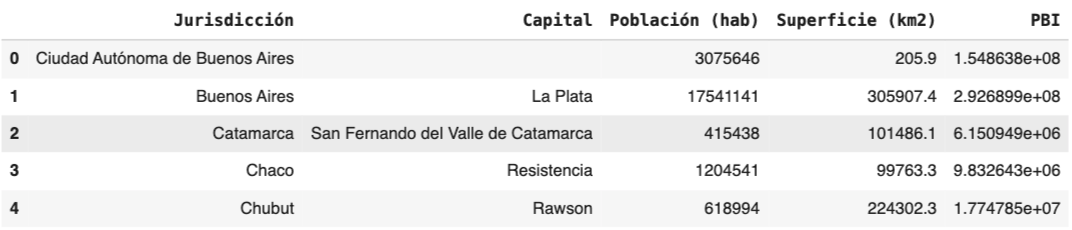
\includegraphics{./imgs/unidad_6/pandas.png}

}

\caption{Esquema de figuras y axes}

\end{figure}%

Pandas incorpora dos estructuras de datos llamados: \textbf{Series} y
\textbf{DataFrames}. Los vamos a ver a continuación.

\subsection{\texorpdfstring{\textbf{Serie}}{Serie}}\label{serie}

Una \textbf{serie} es un vector \textbf{(unidimensional)} capaz de
contener cualquier tipo de dato, como por ejemplo, números enteros o
decimales, strings, objetos de Python, etc.

Para crearlas, se puede partir de un escalar, una lista, un diccionario,
etc., utilizando \texttt{pd.Serie()}:

\begin{Shaded}
\begin{Highlighting}[]
\CommentTok{\# Crear serie partiendo de una lista:}
\NormalTok{lista }\OperatorTok{=}\NormalTok{ [}\DecValTok{1}\NormalTok{, }\StringTok{"a"}\NormalTok{, }\FloatTok{3.5}\NormalTok{]}

\NormalTok{pd.Series(lista)}
\end{Highlighting}
\end{Shaded}

\begin{verbatim}
/Users/aldanarastrelli/Library/Python/3.11/lib/python/site-packages/IPython/core/formatters.py:342: FutureWarning:

In future versions `DataFrame.to_latex` is expected to utilise the base implementation of `Styler.to_latex` for formatting and rendering. The arguments signature may therefore change. It is recommended instead to use `DataFrame.style.to_latex` which also contains additional functionality.
\end{verbatim}

\begin{tabular}{ll}
\toprule
{} &    0 \\
\midrule
0 &    1 \\
1 &    a \\
2 &  3.5 \\
\bottomrule
\end{tabular}

Note que se ven dos líneas verticales de datos. A la derecha se observa
una columna con los elementos de la lista antes creada, mientas que a la
izquierda se encuentra el \textbf{índice}, formado por valores desde 0 a
n-1, siendo n la cantidad de elementos. Este índice numérico es el
predefinido, por lo que si se deseara uno particular, se puede
establecer utilizando \texttt{index}.

El índice es de vital importancia ya que permite acceder a los elementos
de la serie. Es por ello que al colocar un índice en particular, su
longitud debe ser acorde al número de elementos de la misma. De lo
contrario, se mostrará un ValueError.

\begin{Shaded}
\begin{Highlighting}[]
\CommentTok{\# Crear serie partiendo de una lista, indicando el índice}
\NormalTok{pd.Series(lista, index }\OperatorTok{=}\NormalTok{ [}\StringTok{"x"}\NormalTok{, }\StringTok{"y"}\NormalTok{, }\StringTok{"z"}\NormalTok{])}
\end{Highlighting}
\end{Shaded}

\begin{verbatim}
/Users/aldanarastrelli/Library/Python/3.11/lib/python/site-packages/IPython/core/formatters.py:342: FutureWarning:

In future versions `DataFrame.to_latex` is expected to utilise the base implementation of `Styler.to_latex` for formatting and rendering. The arguments signature may therefore change. It is recommended instead to use `DataFrame.style.to_latex` which also contains additional functionality.
\end{verbatim}

\begin{tabular}{ll}
\toprule
{} &    0 \\
\midrule
x &    1 \\
y &    a \\
z &  3.5 \\
\bottomrule
\end{tabular}

En el caso de crear Series utilizando diccionarios, sus claves (o keys)
pasan a formar el índice.

\begin{Shaded}
\begin{Highlighting}[]
\CommentTok{\# Crear serie partiendo de un diccionario:}
\NormalTok{diccionario }\OperatorTok{=}\NormalTok{ \{}\StringTok{"x"}\NormalTok{: }\DecValTok{1}\NormalTok{, }\StringTok{"y"}\NormalTok{: }\StringTok{"a"}\NormalTok{, }\StringTok{"z"}\NormalTok{: }\FloatTok{3.5}\NormalTok{\}}

\NormalTok{a }\OperatorTok{=}\NormalTok{ pd.Series(diccionario)}
\NormalTok{a}
\end{Highlighting}
\end{Shaded}

\begin{verbatim}
/Users/aldanarastrelli/Library/Python/3.11/lib/python/site-packages/IPython/core/formatters.py:342: FutureWarning:

In future versions `DataFrame.to_latex` is expected to utilise the base implementation of `Styler.to_latex` for formatting and rendering. The arguments signature may therefore change. It is recommended instead to use `DataFrame.style.to_latex` which also contains additional functionality.
\end{verbatim}

\begin{tabular}{ll}
\toprule
{} &    0 \\
\midrule
x &    1 \\
y &    a \\
z &  3.5 \\
\bottomrule
\end{tabular}

Como ya se debe estar imaginando, para acceder a un elemento de la
serie, se debe indicar el valor del índice o la posición entre
corchetes.

\begin{Shaded}
\begin{Highlighting}[]
\CommentTok{\# Acceder al elemento de índice x:}
\NormalTok{a[}\StringTok{"x"}\NormalTok{]}
\end{Highlighting}
\end{Shaded}

\begin{verbatim}
1
\end{verbatim}

\begin{Shaded}
\begin{Highlighting}[]
\CommentTok{\# Acceder al elemento de posición 0:}
\NormalTok{a[}\DecValTok{0}\NormalTok{]}
\end{Highlighting}
\end{Shaded}

\begin{verbatim}
1
\end{verbatim}

Otra característica interesante de las series (y de los DataFrames, como
se verá a continuación) es la vectorización: así como los arrays, no
requieren recorrer valor por valor en un for para realizar
operaraciones. Por ejemplo:

\begin{Shaded}
\begin{Highlighting}[]
\NormalTok{a }\OperatorTok{+}\NormalTok{ a}
\end{Highlighting}
\end{Shaded}

\begin{tabular}{ll}
\toprule
{} &    0 \\
\midrule
x &    2 \\
y &   aa \\
z &  7.0 \\
\bottomrule
\end{tabular}

\subsection{\texorpdfstring{\textbf{DataFrame}}{DataFrame}}\label{dataframe}

Un \textbf{DataFrame} es una estructura de datos tabular
\textbf{(bidimensional)}, compuesta por filas y columnas, que se asemeja
a una hoja de cálculo de Excel. Para crearlos, se utiliza
\texttt{DataFrame()} y se ingresan diferentes estructuras como arrays,
diccionarios, listas, series u otros dataframes.

En el siguiente ejemplo, se crea un Dataframe partiendo de un
diccionario \textbf{data} para las columnas y de una lista
\textbf{label} para el índice:

\begin{Shaded}
\begin{Highlighting}[]
\NormalTok{data }\OperatorTok{=}\NormalTok{ \{}\StringTok{\textquotesingle{}columna\_1\textquotesingle{}}\NormalTok{: [}\StringTok{\textquotesingle{}a\textquotesingle{}}\NormalTok{, }\StringTok{\textquotesingle{}b\textquotesingle{}}\NormalTok{, }\StringTok{\textquotesingle{}c\textquotesingle{}}\NormalTok{, }\StringTok{\textquotesingle{}d\textquotesingle{}}\NormalTok{, }\StringTok{\textquotesingle{}e\textquotesingle{}}\NormalTok{, }\StringTok{\textquotesingle{}f\textquotesingle{}}\NormalTok{],}
        \StringTok{\textquotesingle{}columna\_2\textquotesingle{}}\NormalTok{: [}\FloatTok{2.5}\NormalTok{, }\DecValTok{3}\NormalTok{, }\FloatTok{0.5}\NormalTok{, }\VariableTok{None}\NormalTok{, }\DecValTok{5}\NormalTok{, }\VariableTok{None}\NormalTok{],}
        \StringTok{\textquotesingle{}columna\_3\textquotesingle{}}\NormalTok{: [}\DecValTok{1}\NormalTok{, }\DecValTok{3}\NormalTok{, }\DecValTok{2}\NormalTok{, }\DecValTok{3}\NormalTok{, }\DecValTok{2}\NormalTok{, }\DecValTok{3}\NormalTok{]\}}

\NormalTok{labels }\OperatorTok{=}\NormalTok{ [}\StringTok{\textquotesingle{}a1\textquotesingle{}}\NormalTok{, }\StringTok{\textquotesingle{}a2\textquotesingle{}}\NormalTok{, }\StringTok{\textquotesingle{}a3\textquotesingle{}}\NormalTok{, }\StringTok{\textquotesingle{}a4\textquotesingle{}}\NormalTok{, }\StringTok{\textquotesingle{}a5\textquotesingle{}}\NormalTok{, }\StringTok{\textquotesingle{}a6\textquotesingle{}}\NormalTok{]}

\NormalTok{pd.DataFrame(data, index}\OperatorTok{=}\NormalTok{labels)}
\end{Highlighting}
\end{Shaded}

\begin{verbatim}
/Users/aldanarastrelli/Library/Python/3.11/lib/python/site-packages/IPython/core/formatters.py:342: FutureWarning:

In future versions `DataFrame.to_latex` is expected to utilise the base implementation of `Styler.to_latex` for formatting and rendering. The arguments signature may therefore change. It is recommended instead to use `DataFrame.style.to_latex` which also contains additional functionality.
\end{verbatim}

\begin{tabular}{llrr}
\toprule
{} & columna\_1 &  columna\_2 &  columna\_3 \\
\midrule
a1 &         a &        2.5 &          1 \\
a2 &         b &        3.0 &          3 \\
a3 &         c &        0.5 &          2 \\
a4 &         d &        NaN &          3 \\
a5 &         e &        5.0 &          2 \\
a6 &         f &        NaN &          3 \\
\bottomrule
\end{tabular}

\subsubsection{Atributos y descripción de un
Dataframe}\label{atributos-y-descripciuxf3n-de-un-dataframe}

A continuación, se observa una tabla con métodos que nos permiten
conocer las características de un determinado DataFrame.

\begin{longtable}[]{@{}ll@{}}
\toprule\noalign{}
Método & Descripción \\
\midrule\noalign{}
\endhead
\bottomrule\noalign{}
\endlastfoot
\texttt{info()} & Resume la información del DataFrame \\
\texttt{shape} & Devuelve una tupla con el número de filas y columnas \\
\texttt{size} & Número de elementos \\
\texttt{columns} & Lista con los nombres de las columnas \\
\texttt{index} & Lista con los nombres de las filas \\
\texttt{dtypes} & Serie con los tipos de datos de las columnas \\
\texttt{head()} & Muestra las primeras filas \\
\texttt{tail()} & Muestra las últimas filas \\
\texttt{df.describe()} & Brinda métricas de las columnas numéricas \\
\end{longtable}

Para ejemplificar los métodos y las funciones de Pandas, usaremos el
\textbf{DataFrame df} definido en la siguiente línea de código.

\begin{Shaded}
\begin{Highlighting}[]
\NormalTok{data }\OperatorTok{=}\NormalTok{ \{}\StringTok{\textquotesingle{}nombre\textquotesingle{}}\NormalTok{: [}\StringTok{\textquotesingle{}José Martínez\textquotesingle{}}\NormalTok{, }\StringTok{\textquotesingle{}Rosa Díaz\textquotesingle{}}\NormalTok{, }\StringTok{\textquotesingle{}Javier Garcíaz\textquotesingle{}}\NormalTok{, }\StringTok{\textquotesingle{}Carmen López\textquotesingle{}}\NormalTok{, }\StringTok{\textquotesingle{}Marisa Collado\textquotesingle{}}\NormalTok{, }\StringTok{\textquotesingle{}Antonio Ruiz\textquotesingle{}}\NormalTok{, }\StringTok{\textquotesingle{}Antonio Fernández\textquotesingle{}}\NormalTok{, }
                   \StringTok{\textquotesingle{}Pilar González\textquotesingle{}}\NormalTok{, }\StringTok{\textquotesingle{}Pedro Tenorio\textquotesingle{}}\NormalTok{, }\StringTok{\textquotesingle{}Santiago Manzano\textquotesingle{}}\NormalTok{, }\StringTok{\textquotesingle{}Macarena Álvarez\textquotesingle{}}\NormalTok{, }\StringTok{\textquotesingle{}José Sanz\textquotesingle{}}\NormalTok{, }\StringTok{\textquotesingle{}Miguel Gutiérrez\textquotesingle{}}\NormalTok{, }\StringTok{\textquotesingle{}Carolina Moreno\textquotesingle{}}\NormalTok{],}
        \StringTok{\textquotesingle{}edad\textquotesingle{}}\NormalTok{: [}\DecValTok{18}\NormalTok{, }\DecValTok{32}\NormalTok{, }\DecValTok{24}\NormalTok{, }\DecValTok{35}\NormalTok{, }\DecValTok{46}\NormalTok{, }\DecValTok{68}\NormalTok{, }\DecValTok{51}\NormalTok{, }\DecValTok{22}\NormalTok{, }\DecValTok{35}\NormalTok{, }\DecValTok{46}\NormalTok{, }\DecValTok{53}\NormalTok{, }\DecValTok{58}\NormalTok{, }\DecValTok{27}\NormalTok{, }\DecValTok{20}\NormalTok{],}
        \StringTok{\textquotesingle{}sexo\textquotesingle{}}\NormalTok{: [}\StringTok{\textquotesingle{}H\textquotesingle{}}\NormalTok{, }\StringTok{\textquotesingle{}M\textquotesingle{}}\NormalTok{, }\StringTok{\textquotesingle{}H\textquotesingle{}}\NormalTok{, }\StringTok{\textquotesingle{}M\textquotesingle{}}\NormalTok{, }\StringTok{\textquotesingle{}M\textquotesingle{}}\NormalTok{, }\StringTok{\textquotesingle{}H\textquotesingle{}}\NormalTok{, }\StringTok{\textquotesingle{}H\textquotesingle{}}\NormalTok{, }\StringTok{\textquotesingle{}M\textquotesingle{}}\NormalTok{, }\StringTok{\textquotesingle{}H\textquotesingle{}}\NormalTok{, }\StringTok{\textquotesingle{}H\textquotesingle{}}\NormalTok{, }\StringTok{\textquotesingle{}M\textquotesingle{}}\NormalTok{, }\StringTok{\textquotesingle{}H\textquotesingle{}}\NormalTok{, }\StringTok{\textquotesingle{}H\textquotesingle{}}\NormalTok{, }\StringTok{\textquotesingle{}M\textquotesingle{}}\NormalTok{],}
        \StringTok{\textquotesingle{}peso\textquotesingle{}}\NormalTok{: [}\FloatTok{85.0}\NormalTok{, }\FloatTok{65.0}\NormalTok{, }\VariableTok{None}\NormalTok{, }\FloatTok{65.0}\NormalTok{, }\FloatTok{51.0}\NormalTok{, }\FloatTok{66.0}\NormalTok{, }\FloatTok{62.0}\NormalTok{, }\FloatTok{60.0}\NormalTok{, }\FloatTok{90.0}\NormalTok{, }\FloatTok{75.0}\NormalTok{, }\FloatTok{55.0}\NormalTok{, }\FloatTok{78.0}\NormalTok{, }\FloatTok{109.0}\NormalTok{, }\FloatTok{61.0}\NormalTok{],}
        \StringTok{\textquotesingle{}altura\textquotesingle{}}\NormalTok{: [}\FloatTok{1.79}\NormalTok{, }\FloatTok{1.73}\NormalTok{, }\FloatTok{1.81}\NormalTok{, }\FloatTok{1.7}\NormalTok{, }\FloatTok{1.58}\NormalTok{, }\FloatTok{1.74}\NormalTok{, }\FloatTok{1.72}\NormalTok{, }\FloatTok{1.66}\NormalTok{, }\FloatTok{1.94}\NormalTok{, }\FloatTok{1.85}\NormalTok{, }\FloatTok{1.62}\NormalTok{, }\FloatTok{1.87}\NormalTok{, }\FloatTok{1.98}\NormalTok{, }\FloatTok{1.77}\NormalTok{],}
        \StringTok{\textquotesingle{}colesterol\textquotesingle{}}\NormalTok{: [}\FloatTok{182.0}\NormalTok{, }\FloatTok{232.0}\NormalTok{, }\FloatTok{191.0}\NormalTok{, }\FloatTok{200.0}\NormalTok{, }\FloatTok{148.0}\NormalTok{, }\FloatTok{249.0}\NormalTok{, }\FloatTok{276.0}\NormalTok{, }\VariableTok{None}\NormalTok{, }\FloatTok{241.0}\NormalTok{, }\FloatTok{280.0}\NormalTok{, }\FloatTok{262.0}\NormalTok{, }\FloatTok{198.0}\NormalTok{, }\FloatTok{210.0}\NormalTok{, }\FloatTok{194.0}\NormalTok{]\}}

\NormalTok{df }\OperatorTok{=}\NormalTok{ pd.DataFrame(data)}
\NormalTok{df}
\end{Highlighting}
\end{Shaded}

\begin{verbatim}
/Users/aldanarastrelli/Library/Python/3.11/lib/python/site-packages/IPython/core/formatters.py:342: FutureWarning:

In future versions `DataFrame.to_latex` is expected to utilise the base implementation of `Styler.to_latex` for formatting and rendering. The arguments signature may therefore change. It is recommended instead to use `DataFrame.style.to_latex` which also contains additional functionality.
\end{verbatim}

\begin{tabular}{llrlrrr}
\toprule
{} &             nombre &  edad & sexo &   peso &  altura &  colesterol \\
\midrule
0  &      José Martínez &    18 &    H &   85.0 &    1.79 &       182.0 \\
1  &          Rosa Díaz &    32 &    M &   65.0 &    1.73 &       232.0 \\
2  &     Javier Garcíaz &    24 &    H &    NaN &    1.81 &       191.0 \\
3  &       Carmen López &    35 &    M &   65.0 &    1.70 &       200.0 \\
4  &     Marisa Collado &    46 &    M &   51.0 &    1.58 &       148.0 \\
5  &       Antonio Ruiz &    68 &    H &   66.0 &    1.74 &       249.0 \\
6  &  Antonio Fernández &    51 &    H &   62.0 &    1.72 &       276.0 \\
7  &     Pilar González &    22 &    M &   60.0 &    1.66 &         NaN \\
8  &      Pedro Tenorio &    35 &    H &   90.0 &    1.94 &       241.0 \\
9  &   Santiago Manzano &    46 &    H &   75.0 &    1.85 &       280.0 \\
10 &   Macarena Álvarez &    53 &    M &   55.0 &    1.62 &       262.0 \\
11 &          José Sanz &    58 &    H &   78.0 &    1.87 &       198.0 \\
12 &   Miguel Gutiérrez &    27 &    H &  109.0 &    1.98 &       210.0 \\
13 &    Carolina Moreno &    20 &    M &   61.0 &    1.77 &       194.0 \\
\bottomrule
\end{tabular}

\paragraph{Info}\label{info}

Con \texttt{info()} se puede ver: - el índice en la primera línea, que
es un rango de 0 a 13 - el número total de columnas en la segunda línea
- el uso de la memoria en la última - una tabla con los nombres de las
columnas en \textbf{Column}, la cantidad de valores no nulos en
\textbf{Non-Null Count} y el tipo de dato en \textbf{Dtype} para cada
una de ellas.

\begin{Shaded}
\begin{Highlighting}[]
\NormalTok{df.info()}
\end{Highlighting}
\end{Shaded}

\begin{verbatim}
<class 'pandas.core.frame.DataFrame'>
RangeIndex: 14 entries, 0 to 13
Data columns (total 6 columns):
 #   Column      Non-Null Count  Dtype  
---  ------      --------------  -----  
 0   nombre      14 non-null     object 
 1   edad        14 non-null     int64  
 2   sexo        14 non-null     object 
 3   peso        13 non-null     float64
 4   altura      14 non-null     float64
 5   colesterol  13 non-null     float64
dtypes: float64(3), int64(1), object(2)
memory usage: 804.0+ bytes
\end{verbatim}

Note que utilizando \texttt{dtypes}, \texttt{columns} e \texttt{index}
se obtiene parte de esta información:

\begin{Shaded}
\begin{Highlighting}[]
\CommentTok{\# Tipo de dato por columna}
\NormalTok{df.dtypes}
\end{Highlighting}
\end{Shaded}

\begin{verbatim}
/Users/aldanarastrelli/Library/Python/3.11/lib/python/site-packages/IPython/core/formatters.py:342: FutureWarning:

In future versions `DataFrame.to_latex` is expected to utilise the base implementation of `Styler.to_latex` for formatting and rendering. The arguments signature may therefore change. It is recommended instead to use `DataFrame.style.to_latex` which also contains additional functionality.
\end{verbatim}

\begin{tabular}{ll}
\toprule
{} &        0 \\
\midrule
nombre     &   object \\
edad       &    int64 \\
sexo       &   object \\
peso       &  float64 \\
altura     &  float64 \\
colesterol &  float64 \\
\bottomrule
\end{tabular}

\begin{Shaded}
\begin{Highlighting}[]
\CommentTok{\# Nombre de cada columna}
\NormalTok{df.columns}
\end{Highlighting}
\end{Shaded}

\begin{verbatim}
Index(['nombre', 'edad', 'sexo', 'peso', 'altura', 'colesterol'], dtype='object')
\end{verbatim}

\begin{Shaded}
\begin{Highlighting}[]
\CommentTok{\# índice}
\NormalTok{df.index}
\end{Highlighting}
\end{Shaded}

\begin{verbatim}
RangeIndex(start=0, stop=14, step=1)
\end{verbatim}

\paragraph{Shape}\label{shape}

La forma del DataFrame es de 14 filas y 6 columnas, por lo que contiene
84 elementos.

\begin{Shaded}
\begin{Highlighting}[]
\CommentTok{\# Forma del DataFrame (filas, columnas)}
\NormalTok{df.shape}
\end{Highlighting}
\end{Shaded}

\begin{verbatim}
(14, 6)
\end{verbatim}

\begin{Shaded}
\begin{Highlighting}[]
\CommentTok{\# Número de elementos del DataFrame}
\NormalTok{df.size}
\end{Highlighting}
\end{Shaded}

\begin{verbatim}
84
\end{verbatim}

\paragraph{Head}\label{head}

Asimismo, cuando no conocemos un DataFrame, puede ser importante ver las
primeras 5 filas con \texttt{head()} o las últimas con \texttt{tail()}.
Si se quisiera observar un número determinado, sólo hay que
especificarlo, por ejemplo:

\begin{Shaded}
\begin{Highlighting}[]
\CommentTok{\# Mostrar las primeras 3 filas.}
\NormalTok{df.head(}\DecValTok{3}\NormalTok{)}
\end{Highlighting}
\end{Shaded}

\begin{verbatim}
/Users/aldanarastrelli/Library/Python/3.11/lib/python/site-packages/IPython/core/formatters.py:342: FutureWarning:

In future versions `DataFrame.to_latex` is expected to utilise the base implementation of `Styler.to_latex` for formatting and rendering. The arguments signature may therefore change. It is recommended instead to use `DataFrame.style.to_latex` which also contains additional functionality.
\end{verbatim}

\begin{tabular}{llrlrrr}
\toprule
{} &          nombre &  edad & sexo &  peso &  altura &  colesterol \\
\midrule
0 &   José Martínez &    18 &    H &  85.0 &    1.79 &       182.0 \\
1 &       Rosa Díaz &    32 &    M &  65.0 &    1.73 &       232.0 \\
2 &  Javier Garcíaz &    24 &    H &   NaN &    1.81 &       191.0 \\
\bottomrule
\end{tabular}

\begin{Shaded}
\begin{Highlighting}[]
\CommentTok{\# Mostrar las últimas 5 filas.}
\NormalTok{df.tail()}
\end{Highlighting}
\end{Shaded}

\begin{verbatim}
/Users/aldanarastrelli/Library/Python/3.11/lib/python/site-packages/IPython/core/formatters.py:342: FutureWarning:

In future versions `DataFrame.to_latex` is expected to utilise the base implementation of `Styler.to_latex` for formatting and rendering. The arguments signature may therefore change. It is recommended instead to use `DataFrame.style.to_latex` which also contains additional functionality.
\end{verbatim}

\begin{tabular}{llrlrrr}
\toprule
{} &            nombre &  edad & sexo &   peso &  altura &  colesterol \\
\midrule
9  &  Santiago Manzano &    46 &    H &   75.0 &    1.85 &       280.0 \\
10 &  Macarena Álvarez &    53 &    M &   55.0 &    1.62 &       262.0 \\
11 &         José Sanz &    58 &    H &   78.0 &    1.87 &       198.0 \\
12 &  Miguel Gutiérrez &    27 &    H &  109.0 &    1.98 &       210.0 \\
13 &   Carolina Moreno &    20 &    M &   61.0 &    1.77 &       194.0 \\
\bottomrule
\end{tabular}

\paragraph{Describe}\label{describe}

Por otro lado, \texttt{describe()} devuelve un resumen descriptivo de
las columnas de valores numéricos, como ``edad'', ``peso'', ``altura'' y
``colesterol''.

\begin{Shaded}
\begin{Highlighting}[]
\NormalTok{df.describe()}
\end{Highlighting}
\end{Shaded}

\begin{verbatim}
/Users/aldanarastrelli/Library/Python/3.11/lib/python/site-packages/IPython/core/formatters.py:342: FutureWarning:

In future versions `DataFrame.to_latex` is expected to utilise the base implementation of `Styler.to_latex` for formatting and rendering. The arguments signature may therefore change. It is recommended instead to use `DataFrame.style.to_latex` which also contains additional functionality.
\end{verbatim}

\begin{tabular}{lrrrr}
\toprule
{} &       edad &        peso &     altura &  colesterol \\
\midrule
count &  14.000000 &   13.000000 &  14.000000 &   13.000000 \\
mean  &  38.214286 &   70.923077 &   1.768571 &  220.230769 \\
std   &  15.621379 &   16.126901 &   0.115016 &   39.847948 \\
min   &  18.000000 &   51.000000 &   1.580000 &  148.000000 \\
25\%   &  24.750000 &   61.000000 &   1.705000 &  194.000000 \\
50\%   &  35.000000 &   65.000000 &   1.755000 &  210.000000 \\
75\%   &  49.750000 &   78.000000 &   1.840000 &  249.000000 \\
max   &  68.000000 &  109.000000 &   1.980000 &  280.000000 \\
\bottomrule
\end{tabular}

Estas métricas podrían obtenerse utilizando funciones determinadas,
como:\\

\begin{itemize}
\tightlist
\item
  \texttt{count()}: contabiliza los valores no nulos
\item
  \texttt{mean()}: promedio
\item
  \texttt{min()}: valor mínimo
\item
  \texttt{max()}: valor máximo
\end{itemize}

Por ejemplo:

\begin{Shaded}
\begin{Highlighting}[]
\NormalTok{df.count()}
\end{Highlighting}
\end{Shaded}

\begin{verbatim}
/Users/aldanarastrelli/Library/Python/3.11/lib/python/site-packages/IPython/core/formatters.py:342: FutureWarning:

In future versions `DataFrame.to_latex` is expected to utilise the base implementation of `Styler.to_latex` for formatting and rendering. The arguments signature may therefore change. It is recommended instead to use `DataFrame.style.to_latex` which also contains additional functionality.
\end{verbatim}

\begin{tabular}{lr}
\toprule
{} &   0 \\
\midrule
nombre     &  14 \\
edad       &  14 \\
sexo       &  14 \\
peso       &  13 \\
altura     &  14 \\
colesterol &  13 \\
\bottomrule
\end{tabular}

Finalmente, como ocurre con las series, \textbf{para acceder a los
elementos de un DataFrame se puede indicar la posición o el nombre de la
fila o columna}.

Para acceder a una \textbf{fila} en particular, utilizamos
\texttt{iloc{[}{]}} con un entero, una lista de enteros o un rango de
números que indican las posiciones o con \texttt{loc{[}{]}} indicando el
valor del índice.

\begin{Shaded}
\begin{Highlighting}[]
\CommentTok{\# Mostrar los datos de la fila de posición 0:}
\NormalTok{df.iloc[}\DecValTok{0}\NormalTok{]}
\end{Highlighting}
\end{Shaded}

\begin{tabular}{ll}
\toprule
{} &              0 \\
\midrule
nombre     &  José Martínez \\
edad       &             18 \\
sexo       &              H \\
peso       &           85.0 \\
altura     &           1.79 \\
colesterol &          182.0 \\
\bottomrule
\end{tabular}

\begin{Shaded}
\begin{Highlighting}[]
\CommentTok{\# Mostrar la fila de posición 0:}
\NormalTok{df.iloc[[}\DecValTok{0}\NormalTok{]]}
\end{Highlighting}
\end{Shaded}

\begin{verbatim}
/Users/aldanarastrelli/Library/Python/3.11/lib/python/site-packages/IPython/core/formatters.py:342: FutureWarning:

In future versions `DataFrame.to_latex` is expected to utilise the base implementation of `Styler.to_latex` for formatting and rendering. The arguments signature may therefore change. It is recommended instead to use `DataFrame.style.to_latex` which also contains additional functionality.
\end{verbatim}

\begin{tabular}{llrlrrr}
\toprule
{} &         nombre &  edad & sexo &  peso &  altura &  colesterol \\
\midrule
0 &  José Martínez &    18 &    H &  85.0 &    1.79 &       182.0 \\
\bottomrule
\end{tabular}

\begin{Shaded}
\begin{Highlighting}[]
\CommentTok{\# Mostrar las filas de posición 0 y 3:}
\NormalTok{df.iloc[[}\DecValTok{0}\NormalTok{, }\DecValTok{3}\NormalTok{]]}
\end{Highlighting}
\end{Shaded}

\begin{verbatim}
/Users/aldanarastrelli/Library/Python/3.11/lib/python/site-packages/IPython/core/formatters.py:342: FutureWarning:

In future versions `DataFrame.to_latex` is expected to utilise the base implementation of `Styler.to_latex` for formatting and rendering. The arguments signature may therefore change. It is recommended instead to use `DataFrame.style.to_latex` which also contains additional functionality.
\end{verbatim}

\begin{tabular}{llrlrrr}
\toprule
{} &         nombre &  edad & sexo &  peso &  altura &  colesterol \\
\midrule
0 &  José Martínez &    18 &    H &  85.0 &    1.79 &       182.0 \\
3 &   Carmen López &    35 &    M &  65.0 &    1.70 &       200.0 \\
\bottomrule
\end{tabular}

\begin{Shaded}
\begin{Highlighting}[]
\CommentTok{\# Mostrar las filas de posiciones entre 0 hasta 3 (exclusive):}
\NormalTok{df.iloc[:}\DecValTok{3}\NormalTok{]}
\end{Highlighting}
\end{Shaded}

\begin{verbatim}
/Users/aldanarastrelli/Library/Python/3.11/lib/python/site-packages/IPython/core/formatters.py:342: FutureWarning:

In future versions `DataFrame.to_latex` is expected to utilise the base implementation of `Styler.to_latex` for formatting and rendering. The arguments signature may therefore change. It is recommended instead to use `DataFrame.style.to_latex` which also contains additional functionality.
\end{verbatim}

\begin{tabular}{llrlrrr}
\toprule
{} &          nombre &  edad & sexo &  peso &  altura &  colesterol \\
\midrule
0 &   José Martínez &    18 &    H &  85.0 &    1.79 &       182.0 \\
1 &       Rosa Díaz &    32 &    M &  65.0 &    1.73 &       232.0 \\
2 &  Javier Garcíaz &    24 &    H &   NaN &    1.81 &       191.0 \\
\bottomrule
\end{tabular}

\begin{Shaded}
\begin{Highlighting}[]
\CommentTok{\# Equivalente a df.iloc[:3]:}
\NormalTok{df.head(}\DecValTok{3}\NormalTok{)}
\end{Highlighting}
\end{Shaded}

\begin{verbatim}
/Users/aldanarastrelli/Library/Python/3.11/lib/python/site-packages/IPython/core/formatters.py:342: FutureWarning:

In future versions `DataFrame.to_latex` is expected to utilise the base implementation of `Styler.to_latex` for formatting and rendering. The arguments signature may therefore change. It is recommended instead to use `DataFrame.style.to_latex` which also contains additional functionality.
\end{verbatim}

\begin{tabular}{llrlrrr}
\toprule
{} &          nombre &  edad & sexo &  peso &  altura &  colesterol \\
\midrule
0 &   José Martínez &    18 &    H &  85.0 &    1.79 &       182.0 \\
1 &       Rosa Díaz &    32 &    M &  65.0 &    1.73 &       232.0 \\
2 &  Javier Garcíaz &    24 &    H &   NaN &    1.81 &       191.0 \\
\bottomrule
\end{tabular}

\begin{Shaded}
\begin{Highlighting}[]
\CommentTok{\# Mostar la fila cuyo valor del índice es 0:}
\NormalTok{df.loc[}\DecValTok{0}\NormalTok{]}
\end{Highlighting}
\end{Shaded}

\begin{tabular}{ll}
\toprule
{} &              0 \\
\midrule
nombre     &  José Martínez \\
edad       &             18 \\
sexo       &              H \\
peso       &           85.0 \\
altura     &           1.79 \\
colesterol &          182.0 \\
\bottomrule
\end{tabular}

\paragraph{Accediendo a columnas}\label{accediendo-a-columnas}

Por otro lado, para acceder a una \textbf{columna} se pueden utilizar
los nombres de la mismas con \texttt{DataFrame{[}columna{]}} o su
equivalente \texttt{DataFrame.columna}.

\begin{Shaded}
\begin{Highlighting}[]
\CommentTok{\# Mostrar la columna "nombre"}
\NormalTok{df[[}\StringTok{\textquotesingle{}nombre\textquotesingle{}}\NormalTok{]] }\CommentTok{\# o df.nombre}
\end{Highlighting}
\end{Shaded}

\begin{verbatim}
/Users/aldanarastrelli/Library/Python/3.11/lib/python/site-packages/IPython/core/formatters.py:342: FutureWarning:

In future versions `DataFrame.to_latex` is expected to utilise the base implementation of `Styler.to_latex` for formatting and rendering. The arguments signature may therefore change. It is recommended instead to use `DataFrame.style.to_latex` which also contains additional functionality.
\end{verbatim}

\begin{tabular}{ll}
\toprule
{} &             nombre \\
\midrule
0  &      José Martínez \\
1  &          Rosa Díaz \\
2  &     Javier Garcíaz \\
3  &       Carmen López \\
4  &     Marisa Collado \\
5  &       Antonio Ruiz \\
6  &  Antonio Fernández \\
7  &     Pilar González \\
8  &      Pedro Tenorio \\
9  &   Santiago Manzano \\
10 &   Macarena Álvarez \\
11 &          José Sanz \\
12 &   Miguel Gutiérrez \\
13 &    Carolina Moreno \\
\bottomrule
\end{tabular}

\begin{Shaded}
\begin{Highlighting}[]
\CommentTok{\# Mostrar más de una columna: "nombre" y "edad":}
\NormalTok{df[[}\StringTok{\textquotesingle{}nombre\textquotesingle{}}\NormalTok{, }\StringTok{\textquotesingle{}edad\textquotesingle{}}\NormalTok{]]}
\end{Highlighting}
\end{Shaded}

\begin{verbatim}
/Users/aldanarastrelli/Library/Python/3.11/lib/python/site-packages/IPython/core/formatters.py:342: FutureWarning:

In future versions `DataFrame.to_latex` is expected to utilise the base implementation of `Styler.to_latex` for formatting and rendering. The arguments signature may therefore change. It is recommended instead to use `DataFrame.style.to_latex` which also contains additional functionality.
\end{verbatim}

\begin{tabular}{llr}
\toprule
{} &             nombre &  edad \\
\midrule
0  &      José Martínez &    18 \\
1  &          Rosa Díaz &    32 \\
2  &     Javier Garcíaz &    24 \\
3  &       Carmen López &    35 \\
4  &     Marisa Collado &    46 \\
5  &       Antonio Ruiz &    68 \\
6  &  Antonio Fernández &    51 \\
7  &     Pilar González &    22 \\
8  &      Pedro Tenorio &    35 \\
9  &   Santiago Manzano &    46 \\
10 &   Macarena Álvarez &    53 \\
11 &          José Sanz &    58 \\
12 &   Miguel Gutiérrez &    27 \\
13 &    Carolina Moreno &    20 \\
\bottomrule
\end{tabular}

Finalmente, se puede utilizar \texttt{loc{[}filas,\ columnas{]}} que
devuelve un DataFrame con los elemento que se encuentra en las filas con
los nombres de la lista filas y las columnas con los nombres de la lista
columna.

\begin{Shaded}
\begin{Highlighting}[]
\CommentTok{\# Mostrar la filas de índice 0, 1, 2, 3, columnas "nombre" y "edad"}
\NormalTok{df.loc[:}\DecValTok{3}\NormalTok{, [}\StringTok{\textquotesingle{}nombre\textquotesingle{}}\NormalTok{, }\StringTok{\textquotesingle{}edad\textquotesingle{}}\NormalTok{]]}
\end{Highlighting}
\end{Shaded}

\begin{verbatim}
/Users/aldanarastrelli/Library/Python/3.11/lib/python/site-packages/IPython/core/formatters.py:342: FutureWarning:

In future versions `DataFrame.to_latex` is expected to utilise the base implementation of `Styler.to_latex` for formatting and rendering. The arguments signature may therefore change. It is recommended instead to use `DataFrame.style.to_latex` which also contains additional functionality.
\end{verbatim}

\begin{tabular}{llr}
\toprule
{} &          nombre &  edad \\
\midrule
0 &   José Martínez &    18 \\
1 &       Rosa Díaz &    32 \\
2 &  Javier Garcíaz &    24 \\
3 &    Carmen López &    35 \\
\bottomrule
\end{tabular}

\begin{Shaded}
\begin{Highlighting}[]
\CommentTok{\# O su equivalente:}
\NormalTok{df.loc[df.index[[}\DecValTok{0}\NormalTok{, }\DecValTok{1}\NormalTok{, }\DecValTok{2}\NormalTok{, }\DecValTok{3}\NormalTok{]], [}\StringTok{\textquotesingle{}nombre\textquotesingle{}}\NormalTok{, }\StringTok{\textquotesingle{}edad\textquotesingle{}}\NormalTok{]]}
\end{Highlighting}
\end{Shaded}

\begin{verbatim}
/Users/aldanarastrelli/Library/Python/3.11/lib/python/site-packages/IPython/core/formatters.py:342: FutureWarning:

In future versions `DataFrame.to_latex` is expected to utilise the base implementation of `Styler.to_latex` for formatting and rendering. The arguments signature may therefore change. It is recommended instead to use `DataFrame.style.to_latex` which also contains additional functionality.
\end{verbatim}

\begin{tabular}{llr}
\toprule
{} &          nombre &  edad \\
\midrule
0 &   José Martínez &    18 \\
1 &       Rosa Díaz &    32 \\
2 &  Javier Garcíaz &    24 \\
3 &    Carmen López &    35 \\
\bottomrule
\end{tabular}

\subsubsection{Modificar un Dataframe}\label{modificar-un-dataframe}

A la hora de modificar un DataFrame puede ser que querramos:\\

\begin{itemize}
\tightlist
\item
  cambiar la estructura del mismo, como los nombres de las columnas y de
  los índices,
\item
  agregar una nueva filas o columna
\item
  reemplazar un dato en una determinada posición.
\end{itemize}

A continuación, se enumeran distintos métodos para llevar a cabo estos
cambios.

\begin{longtable}[]{@{}
  >{\raggedright\arraybackslash}p{(\columnwidth - 2\tabcolsep) * \real{0.5000}}
  >{\raggedright\arraybackslash}p{(\columnwidth - 2\tabcolsep) * \real{0.5000}}@{}}
\toprule\noalign{}
\begin{minipage}[b]{\linewidth}\raggedright
Método
\end{minipage} & \begin{minipage}[b]{\linewidth}\raggedright
Descripción
\end{minipage} \\
\midrule\noalign{}
\endhead
\bottomrule\noalign{}
\endlastfoot
\texttt{set\_index()} & Convierte una determinada columna en el nuevo
índice. \\
\texttt{reset\_index()} & Reestablece el índice predefinido \\
\texttt{rename()} & Renombra las columnas \\
\texttt{insert()} & Agrega columnas \\
\texttt{loc{[}fila{]}} & Agrega una fila en un índice dado \\
\texttt{drop()} & Elimina columnas y filas \\
\texttt{loc{[}fila,\ columna{]}} & Modifica un valor particular dado un
índice y una columna \\
\texttt{map()} & Busca un valor dado en una columna y lo reemplaza \\
\texttt{replace()} & Reemplaza un valor dado en una columna \\
\end{longtable}

\paragraph{Set\_index y reset\_index}\label{set_index-y-reset_index}

Utilizando \texttt{set\_index()} podemos, Por ejemplo, transformar a la
columna ``nombre'' en el nuevo índice, y para volver al predefinido,
usando \texttt{reset\_index()}.

\begin{Shaded}
\begin{Highlighting}[]
\NormalTok{df }\OperatorTok{=}\NormalTok{ df.set\_index(keys }\OperatorTok{=} \StringTok{"nombre"}\NormalTok{)}
\NormalTok{df.head()}
\end{Highlighting}
\end{Shaded}

\begin{verbatim}
/Users/aldanarastrelli/Library/Python/3.11/lib/python/site-packages/IPython/core/formatters.py:342: FutureWarning:

In future versions `DataFrame.to_latex` is expected to utilise the base implementation of `Styler.to_latex` for formatting and rendering. The arguments signature may therefore change. It is recommended instead to use `DataFrame.style.to_latex` which also contains additional functionality.
\end{verbatim}

\begin{tabular}{lrlrrr}
\toprule
{} &  edad & sexo &  peso &  altura &  colesterol \\
nombre         &       &      &       &         &             \\
\midrule
José Martínez  &    18 &    H &  85.0 &    1.79 &       182.0 \\
Rosa Díaz      &    32 &    M &  65.0 &    1.73 &       232.0 \\
Javier Garcíaz &    24 &    H &   NaN &    1.81 &       191.0 \\
Carmen López   &    35 &    M &  65.0 &    1.70 &       200.0 \\
Marisa Collado &    46 &    M &  51.0 &    1.58 &       148.0 \\
\bottomrule
\end{tabular}

\begin{Shaded}
\begin{Highlighting}[]
\NormalTok{df }\OperatorTok{=}\NormalTok{ df.reset\_index()}
\NormalTok{df.head()}
\end{Highlighting}
\end{Shaded}

\begin{verbatim}
/Users/aldanarastrelli/Library/Python/3.11/lib/python/site-packages/IPython/core/formatters.py:342: FutureWarning:

In future versions `DataFrame.to_latex` is expected to utilise the base implementation of `Styler.to_latex` for formatting and rendering. The arguments signature may therefore change. It is recommended instead to use `DataFrame.style.to_latex` which also contains additional functionality.
\end{verbatim}

\begin{tabular}{llrlrrr}
\toprule
{} &          nombre &  edad & sexo &  peso &  altura &  colesterol \\
\midrule
0 &   José Martínez &    18 &    H &  85.0 &    1.79 &       182.0 \\
1 &       Rosa Díaz &    32 &    M &  65.0 &    1.73 &       232.0 \\
2 &  Javier Garcíaz &    24 &    H &   NaN &    1.81 &       191.0 \\
3 &    Carmen López &    35 &    M &  65.0 &    1.70 &       200.0 \\
4 &  Marisa Collado &    46 &    M &  51.0 &    1.58 &       148.0 \\
\bottomrule
\end{tabular}

\paragraph{Rename, insert y drop}\label{rename-insert-y-drop}

Para renombrar una columna, se utiliza
\texttt{rename(columns=\{"nombre\_columna":\ "nuevo\_nombre\_columna"\})}

\begin{Shaded}
\begin{Highlighting}[]
\CommentTok{\# Reemplazo "nombre" por "nombre y apellido"}
\NormalTok{df }\OperatorTok{=}\NormalTok{ df.rename(columns}\OperatorTok{=}\NormalTok{\{}\StringTok{"nombre"}\NormalTok{: }\StringTok{"nombre y apellido"}\NormalTok{\})}
\NormalTok{df.head()}
\end{Highlighting}
\end{Shaded}

\begin{verbatim}
/Users/aldanarastrelli/Library/Python/3.11/lib/python/site-packages/IPython/core/formatters.py:342: FutureWarning:

In future versions `DataFrame.to_latex` is expected to utilise the base implementation of `Styler.to_latex` for formatting and rendering. The arguments signature may therefore change. It is recommended instead to use `DataFrame.style.to_latex` which also contains additional functionality.
\end{verbatim}

\begin{tabular}{llrlrrr}
\toprule
{} & nombre y apellido &  edad & sexo &  peso &  altura &  colesterol \\
\midrule
0 &     José Martínez &    18 &    H &  85.0 &    1.79 &       182.0 \\
1 &         Rosa Díaz &    32 &    M &  65.0 &    1.73 &       232.0 \\
2 &    Javier Garcíaz &    24 &    H &   NaN &    1.81 &       191.0 \\
3 &      Carmen López &    35 &    M &  65.0 &    1.70 &       200.0 \\
4 &    Marisa Collado &    46 &    M &  51.0 &    1.58 &       148.0 \\
\bottomrule
\end{tabular}

Para agregar una nueva columna, existe el método \texttt{insert()}, que
requiere indicar La posición de la nueva columna, el nombre de la nueva
columna, y los valores de la misma. Para ello, creamos una lista llamada
\textbf{direccion} con 14 valores, para cada una de las personas del
DataFrame.

\begin{Shaded}
\begin{Highlighting}[]
\CommentTok{\# Valores de la nueva columna}
\NormalTok{direccion }\OperatorTok{=}\NormalTok{ [}\StringTok{"CABA"}\NormalTok{, }\StringTok{"Bs As"}\NormalTok{, }\StringTok{"Bs As"}\NormalTok{, }\StringTok{"Bs As"}\NormalTok{, }\StringTok{"CABA"}\NormalTok{, }\StringTok{"Bs As"}\NormalTok{, }\StringTok{"CABA"}\NormalTok{, }\StringTok{"CABA"}\NormalTok{, }\StringTok{"CABA"}\NormalTok{, }\StringTok{"CABA"}\NormalTok{, }\StringTok{"CABA"}\NormalTok{, }\StringTok{"Bs As"}\NormalTok{, }\StringTok{"CABA"}\NormalTok{, }\StringTok{"CABA"}\NormalTok{]}

\CommentTok{\# Insertar la columna "direccion" en la posición 3:}
\NormalTok{df.insert(}\DecValTok{3}\NormalTok{, }\StringTok{"direccion"}\NormalTok{, direccion)}
\NormalTok{df.head()}
\end{Highlighting}
\end{Shaded}

\begin{verbatim}
/Users/aldanarastrelli/Library/Python/3.11/lib/python/site-packages/IPython/core/formatters.py:342: FutureWarning:

In future versions `DataFrame.to_latex` is expected to utilise the base implementation of `Styler.to_latex` for formatting and rendering. The arguments signature may therefore change. It is recommended instead to use `DataFrame.style.to_latex` which also contains additional functionality.
\end{verbatim}

\begin{tabular}{llrllrrr}
\toprule
{} & nombre y apellido &  edad & sexo & direccion &  peso &  altura &  colesterol \\
\midrule
0 &     José Martínez &    18 &    H &      CABA &  85.0 &    1.79 &       182.0 \\
1 &         Rosa Díaz &    32 &    M &     Bs As &  65.0 &    1.73 &       232.0 \\
2 &    Javier Garcíaz &    24 &    H &     Bs As &   NaN &    1.81 &       191.0 \\
3 &      Carmen López &    35 &    M &     Bs As &  65.0 &    1.70 &       200.0 \\
4 &    Marisa Collado &    46 &    M &      CABA &  51.0 &    1.58 &       148.0 \\
\bottomrule
\end{tabular}

Para agregar una nueva fila, se utiliza el ya conocido
\texttt{loc{[}{]}}, que requiere indicar el índice y los valores de la
misma. Para ello, creamos una lista llamada \textbf{nueva\_fila} con
valores para cada columna del DataFrame.

\begin{Shaded}
\begin{Highlighting}[]
\CommentTok{\# Valores de la nueva fila}
\NormalTok{nueva\_fila }\OperatorTok{=}\NormalTok{ [}\StringTok{\textquotesingle{}Carlos Rivas\textquotesingle{}}\NormalTok{, }\DecValTok{28}\NormalTok{, }\StringTok{\textquotesingle{}H\textquotesingle{}}\NormalTok{, }\StringTok{"Bs As"}\NormalTok{, }\FloatTok{89.0}\NormalTok{, }\FloatTok{1.78}\NormalTok{, }\FloatTok{245.0}\NormalTok{]}

\CommentTok{\# Insertar la fila 14}
\NormalTok{df.loc[}\DecValTok{14}\NormalTok{] }\OperatorTok{=}\NormalTok{ nueva\_fila}
\NormalTok{df.tail()}
\end{Highlighting}
\end{Shaded}

\begin{verbatim}
/Users/aldanarastrelli/Library/Python/3.11/lib/python/site-packages/IPython/core/formatters.py:342: FutureWarning:

In future versions `DataFrame.to_latex` is expected to utilise the base implementation of `Styler.to_latex` for formatting and rendering. The arguments signature may therefore change. It is recommended instead to use `DataFrame.style.to_latex` which also contains additional functionality.
\end{verbatim}

\begin{tabular}{llrllrrr}
\toprule
{} & nombre y apellido &  edad & sexo & direccion &   peso &  altura &  colesterol \\
\midrule
10 &  Macarena Álvarez &    53 &    M &      CABA &   55.0 &    1.62 &       262.0 \\
11 &         José Sanz &    58 &    H &     Bs As &   78.0 &    1.87 &       198.0 \\
12 &  Miguel Gutiérrez &    27 &    H &      CABA &  109.0 &    1.98 &       210.0 \\
13 &   Carolina Moreno &    20 &    M &      CABA &   61.0 &    1.77 &       194.0 \\
14 &      Carlos Rivas &    28 &    H &     Bs As &   89.0 &    1.78 &       245.0 \\
\bottomrule
\end{tabular}

Para eliminar una columna \texttt{(axis=1)} o fila \texttt{(axis=0)}, se
utiliza \texttt{drop()}:

\begin{Shaded}
\begin{Highlighting}[]
\CommentTok{\# Elimino la columna "direccion", equivalente a del df["direccion"]}
\NormalTok{df }\OperatorTok{=}\NormalTok{ df.drop(}\StringTok{\textquotesingle{}direccion\textquotesingle{}}\NormalTok{, axis}\OperatorTok{=}\DecValTok{1}\NormalTok{)  }
\NormalTok{df.head()}
\end{Highlighting}
\end{Shaded}

\begin{verbatim}
/Users/aldanarastrelli/Library/Python/3.11/lib/python/site-packages/IPython/core/formatters.py:342: FutureWarning:

In future versions `DataFrame.to_latex` is expected to utilise the base implementation of `Styler.to_latex` for formatting and rendering. The arguments signature may therefore change. It is recommended instead to use `DataFrame.style.to_latex` which also contains additional functionality.
\end{verbatim}

\begin{tabular}{llrlrrr}
\toprule
{} & nombre y apellido &  edad & sexo &  peso &  altura &  colesterol \\
\midrule
0 &     José Martínez &    18 &    H &  85.0 &    1.79 &       182.0 \\
1 &         Rosa Díaz &    32 &    M &  65.0 &    1.73 &       232.0 \\
2 &    Javier Garcíaz &    24 &    H &   NaN &    1.81 &       191.0 \\
3 &      Carmen López &    35 &    M &  65.0 &    1.70 &       200.0 \\
4 &    Marisa Collado &    46 &    M &  51.0 &    1.58 &       148.0 \\
\bottomrule
\end{tabular}

\begin{Shaded}
\begin{Highlighting}[]
\CommentTok{\# Elimino la fila 14}
\NormalTok{df }\OperatorTok{=}\NormalTok{ df.drop(}\DecValTok{14}\NormalTok{, axis}\OperatorTok{=}\DecValTok{0}\NormalTok{) }
\NormalTok{df.tail()}
\end{Highlighting}
\end{Shaded}

\begin{verbatim}
/Users/aldanarastrelli/Library/Python/3.11/lib/python/site-packages/IPython/core/formatters.py:342: FutureWarning:

In future versions `DataFrame.to_latex` is expected to utilise the base implementation of `Styler.to_latex` for formatting and rendering. The arguments signature may therefore change. It is recommended instead to use `DataFrame.style.to_latex` which also contains additional functionality.
\end{verbatim}

\begin{tabular}{llrlrrr}
\toprule
{} & nombre y apellido &  edad & sexo &   peso &  altura &  colesterol \\
\midrule
9  &  Santiago Manzano &    46 &    H &   75.0 &    1.85 &       280.0 \\
10 &  Macarena Álvarez &    53 &    M &   55.0 &    1.62 &       262.0 \\
11 &         José Sanz &    58 &    H &   78.0 &    1.87 &       198.0 \\
12 &  Miguel Gutiérrez &    27 &    H &  109.0 &    1.98 &       210.0 \\
13 &   Carolina Moreno &    20 &    M &   61.0 &    1.77 &       194.0 \\
\bottomrule
\end{tabular}

\begin{tcolorbox}[enhanced jigsaw, bottomrule=.15mm, leftrule=.75mm, opacityback=0, colback=white, toprule=.15mm, bottomtitle=1mm, opacitybacktitle=0.6, rightrule=.15mm, left=2mm, arc=.35mm, coltitle=black, title=\textcolor{quarto-callout-tip-color}{\faLightbulb}\hspace{0.5em}{\textbf{Agregar columnas con operaciones}}, breakable, toptitle=1mm, colframe=quarto-callout-tip-color-frame, titlerule=0mm, colbacktitle=quarto-callout-tip-color!10!white]

Como se ha mencionado anteriormente, gracias a la \textbf{vectorización}
se pueden agregar columnas partiendo de operaciones entre columnas
existentes en el DataFrame.

\end{tcolorbox}

Por ejemplo, suponga que queremos ingresar una columna el índice de masa
corporal de las personas que se calcula de la siguiente manera:

\[
IMC = \frac{Peso(kg)}{Altura(m)^2}\]

\begin{Shaded}
\begin{Highlighting}[]
\CommentTok{\# Crear la columna "IMC"}
\NormalTok{df[}\StringTok{"IMC"}\NormalTok{] }\OperatorTok{=}\NormalTok{ df[}\StringTok{"peso"}\NormalTok{] }\OperatorTok{/}\NormalTok{ df[}\StringTok{"altura"}\NormalTok{]}\OperatorTok{**}\DecValTok{2}
\NormalTok{df.head()}
\end{Highlighting}
\end{Shaded}

\begin{verbatim}
/Users/aldanarastrelli/Library/Python/3.11/lib/python/site-packages/IPython/core/formatters.py:342: FutureWarning:

In future versions `DataFrame.to_latex` is expected to utilise the base implementation of `Styler.to_latex` for formatting and rendering. The arguments signature may therefore change. It is recommended instead to use `DataFrame.style.to_latex` which also contains additional functionality.
\end{verbatim}

\begin{tabular}{llrlrrrr}
\toprule
{} & nombre y apellido &  edad & sexo &  peso &  altura &  colesterol &        IMC \\
\midrule
0 &     José Martínez &    18 &    H &  85.0 &    1.79 &       182.0 &  26.528510 \\
1 &         Rosa Díaz &    32 &    M &  65.0 &    1.73 &       232.0 &  21.718066 \\
2 &    Javier Garcíaz &    24 &    H &   NaN &    1.81 &       191.0 &        NaN \\
3 &      Carmen López &    35 &    M &  65.0 &    1.70 &       200.0 &  22.491349 \\
4 &    Marisa Collado &    46 &    M &  51.0 &    1.58 &       148.0 &  20.429418 \\
\bottomrule
\end{tabular}

De manera análoga, se puede crear la columna \textbf{dirección} sin
utilizar \texttt{insert()}. Usando la lista \textbf{direccion}:

\begin{Shaded}
\begin{Highlighting}[]
\NormalTok{df[}\StringTok{"direccion"}\NormalTok{] }\OperatorTok{=}\NormalTok{ direccion}
\NormalTok{df.head()}
\end{Highlighting}
\end{Shaded}

\begin{verbatim}
/Users/aldanarastrelli/Library/Python/3.11/lib/python/site-packages/IPython/core/formatters.py:342: FutureWarning:

In future versions `DataFrame.to_latex` is expected to utilise the base implementation of `Styler.to_latex` for formatting and rendering. The arguments signature may therefore change. It is recommended instead to use `DataFrame.style.to_latex` which also contains additional functionality.
\end{verbatim}

\begin{tabular}{llrlrrrrl}
\toprule
{} & nombre y apellido &  edad & sexo &  peso &  altura &  colesterol &        IMC & direccion \\
\midrule
0 &     José Martínez &    18 &    H &  85.0 &    1.79 &       182.0 &  26.528510 &      CABA \\
1 &         Rosa Díaz &    32 &    M &  65.0 &    1.73 &       232.0 &  21.718066 &     Bs As \\
2 &    Javier Garcíaz &    24 &    H &   NaN &    1.81 &       191.0 &        NaN &     Bs As \\
3 &      Carmen López &    35 &    M &  65.0 &    1.70 &       200.0 &  22.491349 &     Bs As \\
4 &    Marisa Collado &    46 &    M &  51.0 &    1.58 &       148.0 &  20.429418 &      CABA \\
\bottomrule
\end{tabular}

Finalmente, \textbf{para cambiar un valor determinado} se utiliza
\texttt{loc{[}{]}}, como por ejemplo, agregar el peso de Javier García
(tercera fila):

\begin{Shaded}
\begin{Highlighting}[]
\NormalTok{df.loc[}\DecValTok{2}\NormalTok{, }\StringTok{\textquotesingle{}peso\textquotesingle{}}\NormalTok{] }\OperatorTok{=} \DecValTok{92}
\NormalTok{df.head()}
\end{Highlighting}
\end{Shaded}

\begin{verbatim}
/Users/aldanarastrelli/Library/Python/3.11/lib/python/site-packages/IPython/core/formatters.py:342: FutureWarning:

In future versions `DataFrame.to_latex` is expected to utilise the base implementation of `Styler.to_latex` for formatting and rendering. The arguments signature may therefore change. It is recommended instead to use `DataFrame.style.to_latex` which also contains additional functionality.
\end{verbatim}

\begin{tabular}{llrlrrrrl}
\toprule
{} & nombre y apellido &  edad & sexo &  peso &  altura &  colesterol &        IMC & direccion \\
\midrule
0 &     José Martínez &    18 &    H &  85.0 &    1.79 &       182.0 &  26.528510 &      CABA \\
1 &         Rosa Díaz &    32 &    M &  65.0 &    1.73 &       232.0 &  21.718066 &     Bs As \\
2 &    Javier Garcíaz &    24 &    H &  92.0 &    1.81 &       191.0 &        NaN &     Bs As \\
3 &      Carmen López &    35 &    M &  65.0 &    1.70 &       200.0 &  22.491349 &     Bs As \\
4 &    Marisa Collado &    46 &    M &  51.0 &    1.58 &       148.0 &  20.429418 &      CABA \\
\bottomrule
\end{tabular}

Para transformar los valores de una columna entera, podemos utilizar
\texttt{map()} pasando un diccionario del estilo
\texttt{\{valor\_viejo:\ valor\_nuevo\}}. Por ejemplo, modificar la
columna ``sexo'' reemplazando ``H'' por ``M'' y ``M'' por ``F'':

\begin{Shaded}
\begin{Highlighting}[]
\NormalTok{df[}\StringTok{\textquotesingle{}sexo\textquotesingle{}}\NormalTok{] }\OperatorTok{=}\NormalTok{ df[}\StringTok{\textquotesingle{}sexo\textquotesingle{}}\NormalTok{].}\BuiltInTok{map}\NormalTok{(\{}\StringTok{\textquotesingle{}H\textquotesingle{}}\NormalTok{: }\StringTok{\textquotesingle{}M\textquotesingle{}}\NormalTok{, }\StringTok{\textquotesingle{}M\textquotesingle{}}\NormalTok{: }\StringTok{\textquotesingle{}F\textquotesingle{}}\NormalTok{\})}
\NormalTok{df.head()}
\end{Highlighting}
\end{Shaded}

\begin{verbatim}
/Users/aldanarastrelli/Library/Python/3.11/lib/python/site-packages/IPython/core/formatters.py:342: FutureWarning:

In future versions `DataFrame.to_latex` is expected to utilise the base implementation of `Styler.to_latex` for formatting and rendering. The arguments signature may therefore change. It is recommended instead to use `DataFrame.style.to_latex` which also contains additional functionality.
\end{verbatim}

\begin{tabular}{llrlrrrrl}
\toprule
{} & nombre y apellido &  edad & sexo &  peso &  altura &  colesterol &        IMC & direccion \\
\midrule
0 &     José Martínez &    18 &    M &  85.0 &    1.79 &       182.0 &  26.528510 &      CABA \\
1 &         Rosa Díaz &    32 &    F &  65.0 &    1.73 &       232.0 &  21.718066 &     Bs As \\
2 &    Javier Garcíaz &    24 &    M &  92.0 &    1.81 &       191.0 &        NaN &     Bs As \\
3 &      Carmen López &    35 &    F &  65.0 &    1.70 &       200.0 &  22.491349 &     Bs As \\
4 &    Marisa Collado &    46 &    F &  51.0 &    1.58 &       148.0 &  20.429418 &      CABA \\
\bottomrule
\end{tabular}

Otra manera sería utilizando \texttt{replace()}, como en la columna
``direccion'' donde se modificó ``Bs As'' por ``Buenos Aires''.

\begin{Shaded}
\begin{Highlighting}[]
\NormalTok{df[}\StringTok{\textquotesingle{}direccion\textquotesingle{}}\NormalTok{] }\OperatorTok{=}\NormalTok{ df[}\StringTok{\textquotesingle{}direccion\textquotesingle{}}\NormalTok{].replace(}\StringTok{\textquotesingle{}Bs As\textquotesingle{}}\NormalTok{, }\StringTok{\textquotesingle{}Buenos Aires\textquotesingle{}}\NormalTok{)}
\NormalTok{df.head()}
\end{Highlighting}
\end{Shaded}

\begin{verbatim}
/Users/aldanarastrelli/Library/Python/3.11/lib/python/site-packages/IPython/core/formatters.py:342: FutureWarning:

In future versions `DataFrame.to_latex` is expected to utilise the base implementation of `Styler.to_latex` for formatting and rendering. The arguments signature may therefore change. It is recommended instead to use `DataFrame.style.to_latex` which also contains additional functionality.
\end{verbatim}

\begin{tabular}{llrlrrrrl}
\toprule
{} & nombre y apellido &  edad & sexo &  peso &  altura &  colesterol &        IMC &     direccion \\
\midrule
0 &     José Martínez &    18 &    M &  85.0 &    1.79 &       182.0 &  26.528510 &          CABA \\
1 &         Rosa Díaz &    32 &    F &  65.0 &    1.73 &       232.0 &  21.718066 &  Buenos Aires \\
2 &    Javier Garcíaz &    24 &    M &  92.0 &    1.81 &       191.0 &        NaN &  Buenos Aires \\
3 &      Carmen López &    35 &    F &  65.0 &    1.70 &       200.0 &  22.491349 &  Buenos Aires \\
4 &    Marisa Collado &    46 &    F &  51.0 &    1.58 &       148.0 &  20.429418 &          CABA \\
\bottomrule
\end{tabular}

\subsubsection{Filtrar un Dataframe}\label{filtrar-un-dataframe}

Para filtrar los elementos de un DataFrame se suelen utilizar
condiciones lógicas. Por ejemplo:

\begin{Shaded}
\begin{Highlighting}[]
\CommentTok{\# Seleccionar aquellas personas menores de 40 años:}
\NormalTok{df[df[}\StringTok{\textquotesingle{}edad\textquotesingle{}}\NormalTok{] }\OperatorTok{\textless{}} \DecValTok{40}\NormalTok{]}
\end{Highlighting}
\end{Shaded}

\begin{verbatim}
/Users/aldanarastrelli/Library/Python/3.11/lib/python/site-packages/IPython/core/formatters.py:342: FutureWarning:

In future versions `DataFrame.to_latex` is expected to utilise the base implementation of `Styler.to_latex` for formatting and rendering. The arguments signature may therefore change. It is recommended instead to use `DataFrame.style.to_latex` which also contains additional functionality.
\end{verbatim}

\begin{tabular}{llrlrrrrl}
\toprule
{} & nombre y apellido &  edad & sexo &   peso &  altura &  colesterol &        IMC &     direccion \\
\midrule
0  &     José Martínez &    18 &    M &   85.0 &    1.79 &       182.0 &  26.528510 &          CABA \\
1  &         Rosa Díaz &    32 &    F &   65.0 &    1.73 &       232.0 &  21.718066 &  Buenos Aires \\
2  &    Javier Garcíaz &    24 &    M &   92.0 &    1.81 &       191.0 &        NaN &  Buenos Aires \\
3  &      Carmen López &    35 &    F &   65.0 &    1.70 &       200.0 &  22.491349 &  Buenos Aires \\
7  &    Pilar González &    22 &    F &   60.0 &    1.66 &         NaN &  21.773842 &          CABA \\
8  &     Pedro Tenorio &    35 &    M &   90.0 &    1.94 &       241.0 &  23.913275 &          CABA \\
12 &  Miguel Gutiérrez &    27 &    M &  109.0 &    1.98 &       210.0 &  27.803285 &          CABA \\
13 &   Carolina Moreno &    20 &    F &   61.0 &    1.77 &       194.0 &  19.470778 &          CABA \\
\bottomrule
\end{tabular}

Cuando se requieren múltiples condiciones, se puede adicionar usando
símbolos como \texttt{\&} para \textbf{intersecciones} y
\texttt{\textbar{}} para \textbf{uniones}. Por ejemplo:

\begin{Shaded}
\begin{Highlighting}[]
\CommentTok{\# Seleccionar aquellas personas de sexo femenino y menores de 40 años:}
\NormalTok{df[(df[}\StringTok{\textquotesingle{}edad\textquotesingle{}}\NormalTok{] }\OperatorTok{\textless{}} \DecValTok{40}\NormalTok{) }\OperatorTok{\&}\NormalTok{ (df[}\StringTok{\textquotesingle{}sexo\textquotesingle{}}\NormalTok{] }\OperatorTok{==} \StringTok{\textquotesingle{}F\textquotesingle{}}\NormalTok{)]}
\end{Highlighting}
\end{Shaded}

\begin{verbatim}
/Users/aldanarastrelli/Library/Python/3.11/lib/python/site-packages/IPython/core/formatters.py:342: FutureWarning:

In future versions `DataFrame.to_latex` is expected to utilise the base implementation of `Styler.to_latex` for formatting and rendering. The arguments signature may therefore change. It is recommended instead to use `DataFrame.style.to_latex` which also contains additional functionality.
\end{verbatim}

\begin{tabular}{llrlrrrrl}
\toprule
{} & nombre y apellido &  edad & sexo &  peso &  altura &  colesterol &        IMC &     direccion \\
\midrule
1  &         Rosa Díaz &    32 &    F &  65.0 &    1.73 &       232.0 &  21.718066 &  Buenos Aires \\
3  &      Carmen López &    35 &    F &  65.0 &    1.70 &       200.0 &  22.491349 &  Buenos Aires \\
7  &    Pilar González &    22 &    F &  60.0 &    1.66 &         NaN &  21.773842 &          CABA \\
13 &   Carolina Moreno &    20 &    F &  61.0 &    1.77 &       194.0 &  19.470778 &          CABA \\
\bottomrule
\end{tabular}

\begin{Shaded}
\begin{Highlighting}[]
\CommentTok{\# Seleccionar aquellas personas cuyo peso es 60kg o 90kg:}
\NormalTok{df[(df[}\StringTok{\textquotesingle{}peso\textquotesingle{}}\NormalTok{] }\OperatorTok{==} \FloatTok{60.0}\NormalTok{) }\OperatorTok{|}\NormalTok{ (df[}\StringTok{\textquotesingle{}peso\textquotesingle{}}\NormalTok{] }\OperatorTok{==} \FloatTok{90.0}\NormalTok{)]}
\end{Highlighting}
\end{Shaded}

\begin{verbatim}
/Users/aldanarastrelli/Library/Python/3.11/lib/python/site-packages/IPython/core/formatters.py:342: FutureWarning:

In future versions `DataFrame.to_latex` is expected to utilise the base implementation of `Styler.to_latex` for formatting and rendering. The arguments signature may therefore change. It is recommended instead to use `DataFrame.style.to_latex` which also contains additional functionality.
\end{verbatim}

\begin{tabular}{llrlrrrrl}
\toprule
{} & nombre y apellido &  edad & sexo &  peso &  altura &  colesterol &        IMC & direccion \\
\midrule
7 &    Pilar González &    22 &    F &  60.0 &    1.66 &         NaN &  21.773842 &      CABA \\
8 &     Pedro Tenorio &    35 &    M &  90.0 &    1.94 &       241.0 &  23.913275 &      CABA \\
\bottomrule
\end{tabular}

Cuando se desea filtrar con un cierto rango en una determinada columna,
se pueden utilizar las condiciones antes mencionadas o la función
\texttt{between()}.

\begin{Shaded}
\begin{Highlighting}[]
\CommentTok{\# Equivalente a df[(df[\textquotesingle{}edad\textquotesingle{}] \textgreater{} 25) \& (df[\textquotesingle{}edad\textquotesingle{}] \textless{} 40)]}
\NormalTok{df[df[}\StringTok{\textquotesingle{}edad\textquotesingle{}}\NormalTok{].between(}\DecValTok{25}\NormalTok{, }\DecValTok{40}\NormalTok{)]}
\end{Highlighting}
\end{Shaded}

\begin{verbatim}
/Users/aldanarastrelli/Library/Python/3.11/lib/python/site-packages/IPython/core/formatters.py:342: FutureWarning:

In future versions `DataFrame.to_latex` is expected to utilise the base implementation of `Styler.to_latex` for formatting and rendering. The arguments signature may therefore change. It is recommended instead to use `DataFrame.style.to_latex` which also contains additional functionality.
\end{verbatim}

\begin{tabular}{llrlrrrrl}
\toprule
{} & nombre y apellido &  edad & sexo &   peso &  altura &  colesterol &        IMC &     direccion \\
\midrule
1  &         Rosa Díaz &    32 &    F &   65.0 &    1.73 &       232.0 &  21.718066 &  Buenos Aires \\
3  &      Carmen López &    35 &    F &   65.0 &    1.70 &       200.0 &  22.491349 &  Buenos Aires \\
8  &     Pedro Tenorio &    35 &    M &   90.0 &    1.94 &       241.0 &  23.913275 &          CABA \\
12 &  Miguel Gutiérrez &    27 &    M &  109.0 &    1.98 &       210.0 &  27.803285 &          CABA \\
\bottomrule
\end{tabular}

Finalmente, puede ser interesante encontrar aquellas las filas con datos
faltantes o \texttt{NaN}. Para ello, se utiliza la función
\texttt{isnull()} que devuelve \texttt{True} si el valor de la columna
es nulo o NaN. Por ejemplo:

\begin{Shaded}
\begin{Highlighting}[]
\NormalTok{df[}\StringTok{\textquotesingle{}IMC\textquotesingle{}}\NormalTok{].isnull()}
\end{Highlighting}
\end{Shaded}

\begin{tabular}{ll}
\toprule
{} &    IMC \\
\midrule
0  &  False \\
1  &  False \\
2  &   True \\
3  &  False \\
4  &  False \\
5  &  False \\
6  &  False \\
7  &  False \\
8  &  False \\
9  &  False \\
10 &  False \\
11 &  False \\
12 &  False \\
13 &  False \\
\bottomrule
\end{tabular}

Para visualizar aquella fila donde el índice de masa corporal es nulo,
filtramos:

\begin{Shaded}
\begin{Highlighting}[]
\NormalTok{df[df[}\StringTok{\textquotesingle{}IMC\textquotesingle{}}\NormalTok{].isnull() }\OperatorTok{==} \VariableTok{True}\NormalTok{]}
\end{Highlighting}
\end{Shaded}

\begin{verbatim}
/Users/aldanarastrelli/Library/Python/3.11/lib/python/site-packages/IPython/core/formatters.py:342: FutureWarning:

In future versions `DataFrame.to_latex` is expected to utilise the base implementation of `Styler.to_latex` for formatting and rendering. The arguments signature may therefore change. It is recommended instead to use `DataFrame.style.to_latex` which also contains additional functionality.
\end{verbatim}

\begin{tabular}{llrlrrrrl}
\toprule
{} & nombre y apellido &  edad & sexo &  peso &  altura &  colesterol &  IMC &     direccion \\
\midrule
2 &    Javier Garcíaz &    24 &    M &  92.0 &    1.81 &       191.0 &  NaN &  Buenos Aires \\
\bottomrule
\end{tabular}

\subsubsection{Otros métodos útiles}\label{otros-muxe9todos-uxfatiles}

A continuación, se muestra una lista con métodos que resultan muy útiles
a la hora de analizar datos:

\begin{longtable}[]{@{}
  >{\raggedright\arraybackslash}p{(\columnwidth - 2\tabcolsep) * \real{0.5000}}
  >{\raggedright\arraybackslash}p{(\columnwidth - 2\tabcolsep) * \real{0.5000}}@{}}
\toprule\noalign{}
\begin{minipage}[b]{\linewidth}\raggedright
Método
\end{minipage} & \begin{minipage}[b]{\linewidth}\raggedright
Descripción
\end{minipage} \\
\midrule\noalign{}
\endhead
\bottomrule\noalign{}
\endlastfoot
\texttt{sort\_values(by,\ ascending)} & Ordena el DataFrame considerando
los valores de la o las columnas determinadas \\
\texttt{value\_counts()} & Indica los valores únicos de una determinada
columna y el número de veces que aparece en ella \\
\texttt{groupby().agg()} & Agrupa las filas según ciertos valores de
columnas y aplica funciones \\
\end{longtable}

\begin{itemize}
\tightlist
\item
  Sort value:
\end{itemize}

Para utilizar la función \texttt{sort\_values(by,\ ascending)}, se debe
indicar en el parámetro \texttt{by} una lista con las columnas para
ordenar el DataFrame y en \texttt{ascending}, \texttt{True} si el orden
deseado es creciente o \texttt{False} para decreciente.

En el siguiente ejemplo ordenamos por ``nombre y apellido'' en forma
alfabética:

\begin{Shaded}
\begin{Highlighting}[]
\NormalTok{df.sort\_values(by}\OperatorTok{=}\NormalTok{[}\StringTok{\textquotesingle{}nombre y apellido\textquotesingle{}}\NormalTok{], ascending}\OperatorTok{=}\NormalTok{[}\VariableTok{True}\NormalTok{])}
\end{Highlighting}
\end{Shaded}

\begin{verbatim}
/Users/aldanarastrelli/Library/Python/3.11/lib/python/site-packages/IPython/core/formatters.py:342: FutureWarning:

In future versions `DataFrame.to_latex` is expected to utilise the base implementation of `Styler.to_latex` for formatting and rendering. The arguments signature may therefore change. It is recommended instead to use `DataFrame.style.to_latex` which also contains additional functionality.
\end{verbatim}

\begin{tabular}{llrlrrrrl}
\toprule
{} &  nombre y apellido &  edad & sexo &   peso &  altura &  colesterol &        IMC &     direccion \\
\midrule
6  &  Antonio Fernández &    51 &    M &   62.0 &    1.72 &       276.0 &  20.957274 &          CABA \\
5  &       Antonio Ruiz &    68 &    M &   66.0 &    1.74 &       249.0 &  21.799445 &  Buenos Aires \\
3  &       Carmen López &    35 &    F &   65.0 &    1.70 &       200.0 &  22.491349 &  Buenos Aires \\
13 &    Carolina Moreno &    20 &    F &   61.0 &    1.77 &       194.0 &  19.470778 &          CABA \\
2  &     Javier Garcíaz &    24 &    M &   92.0 &    1.81 &       191.0 &        NaN &  Buenos Aires \\
0  &      José Martínez &    18 &    M &   85.0 &    1.79 &       182.0 &  26.528510 &          CABA \\
11 &          José Sanz &    58 &    M &   78.0 &    1.87 &       198.0 &  22.305471 &  Buenos Aires \\
10 &   Macarena Álvarez &    53 &    F &   55.0 &    1.62 &       262.0 &  20.957171 &          CABA \\
4  &     Marisa Collado &    46 &    F &   51.0 &    1.58 &       148.0 &  20.429418 &          CABA \\
12 &   Miguel Gutiérrez &    27 &    M &  109.0 &    1.98 &       210.0 &  27.803285 &          CABA \\
8  &      Pedro Tenorio &    35 &    M &   90.0 &    1.94 &       241.0 &  23.913275 &          CABA \\
7  &     Pilar González &    22 &    F &   60.0 &    1.66 &         NaN &  21.773842 &          CABA \\
1  &          Rosa Díaz &    32 &    F &   65.0 &    1.73 &       232.0 &  21.718066 &  Buenos Aires \\
9  &   Santiago Manzano &    46 &    M &   75.0 &    1.85 &       280.0 &  21.913806 &          CABA \\
\bottomrule
\end{tabular}

Ahora, \textbf{¿Qué ocurre cuando ordenamos siguiendo varias columnas?}
Los valores del DataFrame se ordenan siguiendo la primera columna en
primer lugar, luego la segunda, y así sucesivamente.

\begin{Shaded}
\begin{Highlighting}[]
\NormalTok{df.sort\_values(by}\OperatorTok{=}\NormalTok{[}\StringTok{\textquotesingle{}direccion\textquotesingle{}}\NormalTok{, }\StringTok{\textquotesingle{}nombre y apellido\textquotesingle{}}\NormalTok{], ascending}\OperatorTok{=}\NormalTok{[}\VariableTok{True}\NormalTok{, }\VariableTok{True}\NormalTok{])}
\end{Highlighting}
\end{Shaded}

\begin{verbatim}
/Users/aldanarastrelli/Library/Python/3.11/lib/python/site-packages/IPython/core/formatters.py:342: FutureWarning:

In future versions `DataFrame.to_latex` is expected to utilise the base implementation of `Styler.to_latex` for formatting and rendering. The arguments signature may therefore change. It is recommended instead to use `DataFrame.style.to_latex` which also contains additional functionality.
\end{verbatim}

\begin{tabular}{llrlrrrrl}
\toprule
{} &  nombre y apellido &  edad & sexo &   peso &  altura &  colesterol &        IMC &     direccion \\
\midrule
5  &       Antonio Ruiz &    68 &    M &   66.0 &    1.74 &       249.0 &  21.799445 &  Buenos Aires \\
3  &       Carmen López &    35 &    F &   65.0 &    1.70 &       200.0 &  22.491349 &  Buenos Aires \\
2  &     Javier Garcíaz &    24 &    M &   92.0 &    1.81 &       191.0 &        NaN &  Buenos Aires \\
11 &          José Sanz &    58 &    M &   78.0 &    1.87 &       198.0 &  22.305471 &  Buenos Aires \\
1  &          Rosa Díaz &    32 &    F &   65.0 &    1.73 &       232.0 &  21.718066 &  Buenos Aires \\
6  &  Antonio Fernández &    51 &    M &   62.0 &    1.72 &       276.0 &  20.957274 &          CABA \\
13 &    Carolina Moreno &    20 &    F &   61.0 &    1.77 &       194.0 &  19.470778 &          CABA \\
0  &      José Martínez &    18 &    M &   85.0 &    1.79 &       182.0 &  26.528510 &          CABA \\
10 &   Macarena Álvarez &    53 &    F &   55.0 &    1.62 &       262.0 &  20.957171 &          CABA \\
4  &     Marisa Collado &    46 &    F &   51.0 &    1.58 &       148.0 &  20.429418 &          CABA \\
12 &   Miguel Gutiérrez &    27 &    M &  109.0 &    1.98 &       210.0 &  27.803285 &          CABA \\
8  &      Pedro Tenorio &    35 &    M &   90.0 &    1.94 &       241.0 &  23.913275 &          CABA \\
7  &     Pilar González &    22 &    F &   60.0 &    1.66 &         NaN &  21.773842 &          CABA \\
9  &   Santiago Manzano &    46 &    M &   75.0 &    1.85 &       280.0 &  21.913806 &          CABA \\
\bottomrule
\end{tabular}

Analicemos el ejemplo anterior, donde queremos ordenar según
``direccion'' y ``nombre y apellido''. Allí, primero se ordena de manera
creciente por dirección, resultando en dos grupos: el superior con
``direccion'' = ``Buenos Aires'' y el inferior con ``CABA''. Luego, cada
uno de esos grupos se ordena por ``nombre y apellido'' de forma
creciente.

\begin{figure}[H]

{\centering 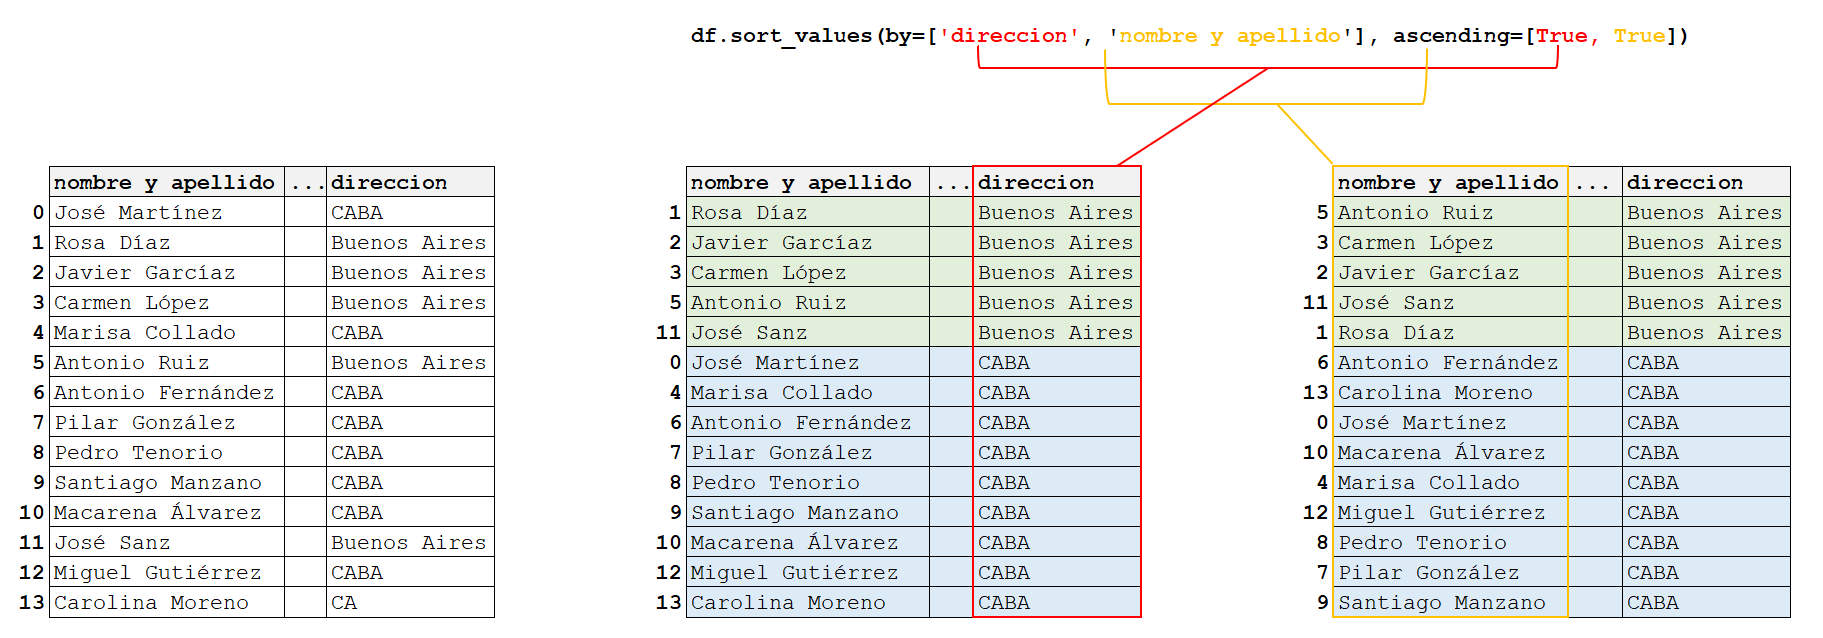
\includegraphics{./imgs/unidad_6/sortvalues.png}

}

\caption{Ejemplo de sort\_values()}

\end{figure}%

\begin{itemize}
\tightlist
\item
  Value Count:
\end{itemize}

Utilizando \texttt{value\_counts()} se pueden contar las filas en cada
grupo según ``direccion''. Es decir, cuantas filas hay para ``Buenos
Aires'' y para ``CABA''.

\begin{Shaded}
\begin{Highlighting}[]
\NormalTok{df[}\StringTok{\textquotesingle{}direccion\textquotesingle{}}\NormalTok{].value\_counts()}
\end{Highlighting}
\end{Shaded}

\begin{verbatim}
/Users/aldanarastrelli/Library/Python/3.11/lib/python/site-packages/IPython/core/formatters.py:342: FutureWarning:

In future versions `DataFrame.to_latex` is expected to utilise the base implementation of `Styler.to_latex` for formatting and rendering. The arguments signature may therefore change. It is recommended instead to use `DataFrame.style.to_latex` which also contains additional functionality.
\end{verbatim}

\begin{tabular}{lr}
\toprule
{} &  direccion \\
\midrule
CABA         &          9 \\
Buenos Aires &          5 \\
\bottomrule
\end{tabular}

\begin{itemize}
\tightlist
\item
  Group by:
\end{itemize}

\texttt{groupby()} es un método que nos permite agrupar los datos del
DataFrame según los valores de una o unas columnas dadas, tranformándose
estas en el nuevo índice de los grupos. Por ejemplo, si quisieramos
agrupar por:

\begin{enumerate}
\def\labelenumi{\arabic{enumi}.}
\item
  ``direccion'': corremos
  \texttt{df.groupby({[}\textquotesingle{}direccion\textquotesingle{}{]})}
  obteniendo una tabla con valores agrupados por ``direccion'', siendo
  esta columna el nuevo índice.
\item
  ``direccion'' y ``sexo'': corremos
  \texttt{df.groupby({[}\textquotesingle{}direccion\textquotesingle{},\ \textquotesingle{}sexo\textquotesingle{}{]})}
  obteniendo una tabla con valores agrupados por ``direccion'' y
  ``sexo'', siendo ambas columnas el nuevo índice.
\end{enumerate}

\begin{figure}[H]

{\centering 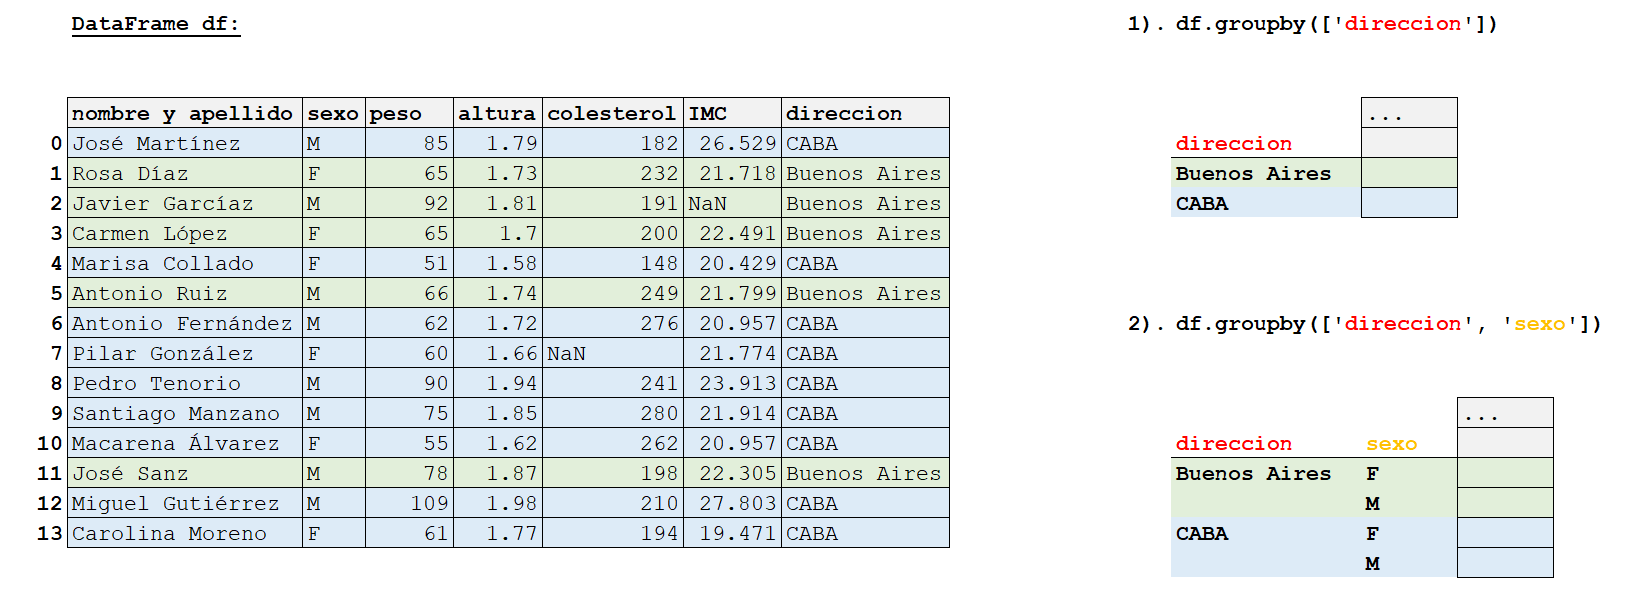
\includegraphics{./imgs/unidad_6/groupby.png}

}

\caption{Ejemplo de groupby()}

\end{figure}%

Una vez obtenidos los grupos que deseamos analizar, podemos realizar una
función de agregación \texttt{agg()} utilizando algunas o todas las
columnas restantes. Estas funciones pueder ser suma, media, mínimo,
máximo, contar valores no nulos, entre otras. Veamos algunos ejemplos:

\begin{Shaded}
\begin{Highlighting}[]
\CommentTok{\# Agrupar por "direccion" y contar los valores no nulos de todas las columnas}
\NormalTok{df.groupby([}\StringTok{\textquotesingle{}direccion\textquotesingle{}}\NormalTok{]).agg(}\StringTok{\textquotesingle{}count\textquotesingle{}}\NormalTok{)}
\end{Highlighting}
\end{Shaded}

\begin{verbatim}
/Users/aldanarastrelli/Library/Python/3.11/lib/python/site-packages/IPython/core/formatters.py:342: FutureWarning:

In future versions `DataFrame.to_latex` is expected to utilise the base implementation of `Styler.to_latex` for formatting and rendering. The arguments signature may therefore change. It is recommended instead to use `DataFrame.style.to_latex` which also contains additional functionality.
\end{verbatim}

\begin{tabular}{lrrrrrrr}
\toprule
{} &  nombre y apellido &  edad &  sexo &  peso &  altura &  colesterol &  IMC \\
direccion    &                    &       &       &       &         &             &      \\
\midrule
Buenos Aires &                  5 &     5 &     5 &     5 &       5 &           5 &    4 \\
CABA         &                  9 &     9 &     9 &     9 &       9 &           8 &    9 \\
\bottomrule
\end{tabular}

\begin{Shaded}
\begin{Highlighting}[]
\CommentTok{\# Agrupar por "direccion" y "sexo" y contar los valores no nulos de alguna columnas}
\NormalTok{df.groupby([}\StringTok{\textquotesingle{}direccion\textquotesingle{}}\NormalTok{, }\StringTok{\textquotesingle{}sexo\textquotesingle{}}\NormalTok{])[[}\StringTok{\textquotesingle{}edad\textquotesingle{}}\NormalTok{, }\StringTok{\textquotesingle{}peso\textquotesingle{}}\NormalTok{]].agg(}\StringTok{\textquotesingle{}count\textquotesingle{}}\NormalTok{)}
\end{Highlighting}
\end{Shaded}

\begin{verbatim}
/Users/aldanarastrelli/Library/Python/3.11/lib/python/site-packages/IPython/core/formatters.py:342: FutureWarning:

In future versions `DataFrame.to_latex` is expected to utilise the base implementation of `Styler.to_latex` for formatting and rendering. The arguments signature may therefore change. It is recommended instead to use `DataFrame.style.to_latex` which also contains additional functionality.
\end{verbatim}

\begin{tabular}{llrr}
\toprule
     &   &  edad &  peso \\
direccion & sexo &       &       \\
\midrule
Buenos Aires & F &     2 &     2 \\
     & M &     3 &     3 \\
CABA & F &     4 &     4 \\
     & M &     5 &     5 \\
\bottomrule
\end{tabular}

También se puede asignar para cada columna, una operación distinta:

\begin{Shaded}
\begin{Highlighting}[]
\CommentTok{\# Agrupar por "direccion" y "sexo" y calcular el valor máximo de la columna "colesterol" y el promedio de "peso"}
\NormalTok{df.groupby([}\StringTok{\textquotesingle{}direccion\textquotesingle{}}\NormalTok{, }\StringTok{\textquotesingle{}sexo\textquotesingle{}}\NormalTok{]).agg(\{}\StringTok{\textquotesingle{}colesterol\textquotesingle{}}\NormalTok{: [}\StringTok{\textquotesingle{}max\textquotesingle{}}\NormalTok{], }\StringTok{\textquotesingle{}peso\textquotesingle{}}\NormalTok{: [}\StringTok{\textquotesingle{}mean\textquotesingle{}}\NormalTok{]\})}
\end{Highlighting}
\end{Shaded}

\begin{verbatim}
/Users/aldanarastrelli/Library/Python/3.11/lib/python/site-packages/IPython/core/formatters.py:342: FutureWarning:

In future versions `DataFrame.to_latex` is expected to utilise the base implementation of `Styler.to_latex` for formatting and rendering. The arguments signature may therefore change. It is recommended instead to use `DataFrame.style.to_latex` which also contains additional functionality.
\end{verbatim}

\begin{tabular}{llrr}
\toprule
     &   & colesterol &       peso \\
     &   &        max &       mean \\
direccion & sexo &            &            \\
\midrule
Buenos Aires & F &      232.0 &  65.000000 \\
     & M &      249.0 &  78.666667 \\
CABA & F &      262.0 &  56.750000 \\
     & M &      280.0 &  84.200000 \\
\bottomrule
\end{tabular}

\begin{Shaded}
\begin{Highlighting}[]
\CommentTok{\# Agrupar por "direccion" y "sexo" y calcular los valores máximos y mínimos de la columna "colesterol" y el promedio de "peso"}
\NormalTok{df.groupby([}\StringTok{\textquotesingle{}direccion\textquotesingle{}}\NormalTok{, }\StringTok{\textquotesingle{}sexo\textquotesingle{}}\NormalTok{]).agg(\{}\StringTok{\textquotesingle{}colesterol\textquotesingle{}}\NormalTok{: [}\StringTok{\textquotesingle{}min\textquotesingle{}}\NormalTok{, }\StringTok{\textquotesingle{}max\textquotesingle{}}\NormalTok{], }\StringTok{\textquotesingle{}peso\textquotesingle{}}\NormalTok{: [}\StringTok{\textquotesingle{}mean\textquotesingle{}}\NormalTok{]\})}
\end{Highlighting}
\end{Shaded}

\begin{verbatim}
/Users/aldanarastrelli/Library/Python/3.11/lib/python/site-packages/IPython/core/formatters.py:342: FutureWarning:

In future versions `DataFrame.to_latex` is expected to utilise the base implementation of `Styler.to_latex` for formatting and rendering. The arguments signature may therefore change. It is recommended instead to use `DataFrame.style.to_latex` which also contains additional functionality.
\end{verbatim}

\begin{tabular}{llrrr}
\toprule
     &   & \multicolumn{2}{l}{colesterol} &       peso \\
     &   &        min &    max &       mean \\
direccion & sexo &            &        &            \\
\midrule
Buenos Aires & F &      200.0 &  232.0 &  65.000000 \\
     & M &      191.0 &  249.0 &  78.666667 \\
CABA & F &      148.0 &  262.0 &  56.750000 \\
     & M &      182.0 &  280.0 &  84.200000 \\
\bottomrule
\end{tabular}

\section{Matplotlib}\label{matplotlib}

Matplotlib es probablemente la biblioteca de Python más usada para crear
gráficos, también llamados \textbf{plots}. Esta provee una forma rápida
de graficar datos en varios formatos de alta calidad que pueden ser
compartidos y/o publicados, resultando una alternativa open source de
MATLAB. De hecho, matplotlib.pyplot es una colección de funciones que
hacen que matplotlib funcione como MATLAB, con comandos análogos y
argumentos similares.

Como ya se imagina, el primer paso es importar la biblioteca. Por
convención:

\begin{Shaded}
\begin{Highlighting}[]
\ImportTok{import}\NormalTok{ matplotlib.pyplot }\ImportTok{as}\NormalTok{ plt}
\end{Highlighting}
\end{Shaded}

\subsection{Creación de gráficos con
matplotlib}\label{creaciuxf3n-de-gruxe1ficos-con-matplotlib}

Para crear un gráfico con matplotlib, se deben seguir los siguientes
pasos:

\begin{enumerate}
\def\labelenumi{\arabic{enumi}.}
\item
  \textbf{Crear la figura} que contendrá el gráfico, utilizando las
  funciones \texttt{subplots()} o \texttt{figure()}. Se recomienda la
  primera, como se verá más adelante.
\item
  \textbf{Graficar los datos}, utilizando distintas funciones
  dependiendo del tipo de gráfico que se desea realizar:
\end{enumerate}

\begin{longtable}[]{@{}ll@{}}
\toprule\noalign{}
Función & Tipo de Gráfico \\
\midrule\noalign{}
\endhead
\bottomrule\noalign{}
\endlastfoot
\texttt{plot()} & Gráfico de línea \\
\texttt{scatter()} & Gráfico de puntos \\
\texttt{bar()} & Gráfico de barras verticales \\
\texttt{barh()} & Gráfico de barras horizontales \\
\texttt{pie()} & Gráfico de torta \\
\end{longtable}

\begin{enumerate}
\def\labelenumi{\arabic{enumi}.}
\setcounter{enumi}{2}
\item
  \textbf{Personalizar el gráfico}. Este paso no es mandatorio, pero sí,
  muy recomendado para lograr un mejor entendimiento de la visualización
\item
  \textbf{Mostrar el gráfico}, utilizando la función \texttt{show()}
\end{enumerate}

Esto quiere decir que, si deseamos visualizar datos rápidamente,
podríamos realizarlo corriendo únicamente las siguientes tres líneas de
código:

\textbf{Opción 1}

\begin{verbatim}
fig = plt.figure()  
plt.funcion_grafico_elegido()       # Reemplazar funcion_grafico_elegido() por una función
plt.show()  
\end{verbatim}

\textbf{Opción 2}

\begin{verbatim}
fig, ax = plt.subplots()  
ax.funcion_grafico_elegido()        # Reemplazar funcion_grafico_elegido() por una función     
plt.show()  
\end{verbatim}

Pero, \textbf{¿cuál debería usar?} Eso depende de lo que quieras hacer.
A continuación, se verá el detalle de lo que está ocurriendo en cada
línea, para que así puedas elegir qué es lo mejor para vos.

\begin{Shaded}
\begin{Highlighting}[]
\NormalTok{plt.figure()}
\end{Highlighting}
\end{Shaded}

\begin{verbatim}
<Figure size 1650x1050 with 0 Axes>
\end{verbatim}

\begin{verbatim}
<Figure size 1650x1050 with 0 Axes>
\end{verbatim}

\begin{Shaded}
\begin{Highlighting}[]
\NormalTok{plt.subplots()}
\end{Highlighting}
\end{Shaded}

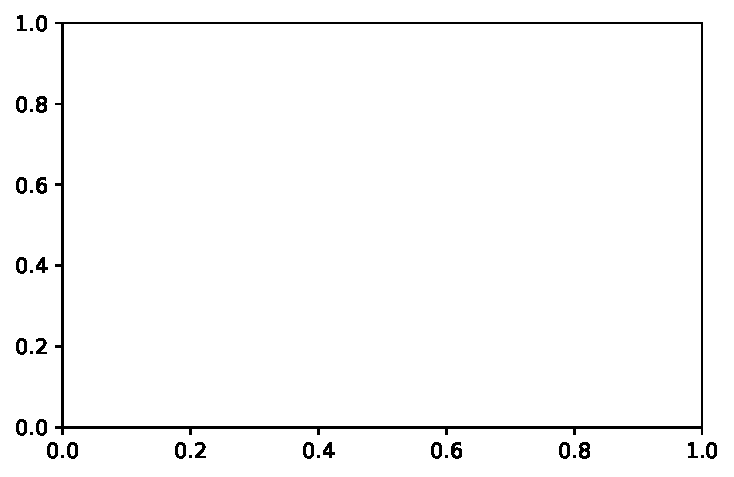
\includegraphics{unidad_6_files/figure-pdf/cell-109-output-1.pdf}

Si bien no se puede ver un gráfico en ninguno de los outputs, analicemos
lo que nos imprime:

\begin{enumerate}
\def\labelenumi{\arabic{enumi}.}
\tightlist
\item
  \texttt{fig\ =\ plt.figure()} crea una \textbf{figura pero sin axes},
  por lo que muestra
  \texttt{\textless{}Figure\ size\ 640x480\ with\ 0\ Axes\textgreater{}}.
\item
  \texttt{fig,\ ax\ =\ plt.subplots()} permite \textbf{crear ambos:
  figura y axes}, por lo que muestra
  \texttt{\textless{}Figure\ size\ 640x480\ with\ 1\ Axes\textgreater{},\ \textless{}AxesSubplot:\ \textgreater{})}.
\end{enumerate}

Note además, que se ha seguido una convención al nombrarse la
\textbf{figura} como \texttt{fig} y los \textbf{axes} como \texttt{ax}.
Pero\ldots{} \textbf{¿qué es una figura y un axes?}

Una \textbf{figura} es el marco que delimita la zona donde se trazan los
gráficos, mientras que los \textbf{axes}, son lo que llamamos comunmente
gráficos, es decir, son las áreas donde los puntos se pueden especificar
en términos de coordenadas. \textbf{Por lo tanto, una figura puede
contener muchos axes, pero un axes determinado sólo puede estar
contenido en una única figura.}

\begin{figure}[H]

{\centering 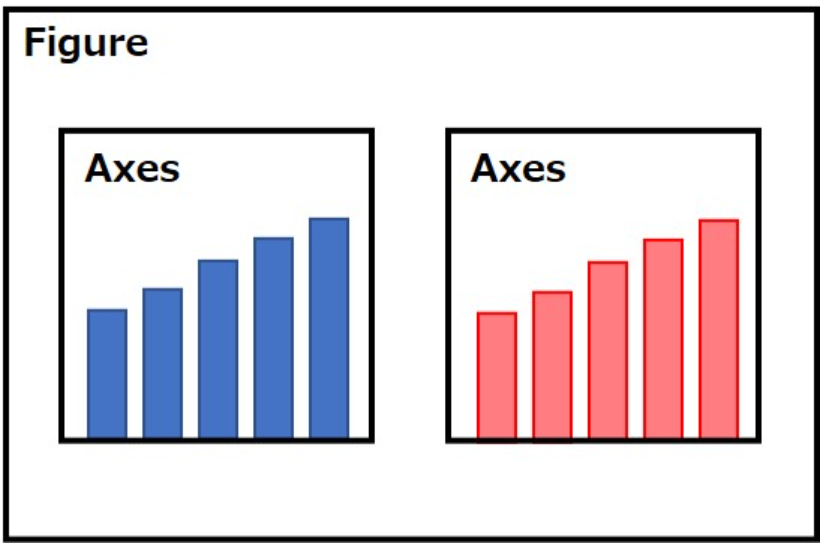
\includegraphics{./imgs/unidad_6/fig_ax.png}

}

\caption{Esquema de figuras y axes}

\end{figure}%

\begin{tcolorbox}[enhanced jigsaw, bottomrule=.15mm, leftrule=.75mm, opacityback=0, colback=white, toprule=.15mm, bottomtitle=1mm, opacitybacktitle=0.6, rightrule=.15mm, left=2mm, arc=.35mm, coltitle=black, title=\textcolor{quarto-callout-note-color}{\faInfo}\hspace{0.5em}{\textbf{¡Ojo! No confundir axes con axis}\\
}, breakable, toptitle=1mm, colframe=quarto-callout-note-color-frame, titlerule=0mm, colbacktitle=quarto-callout-note-color!10!white]

Los \textbf{Axis} son los ejes cartesianos que se encargan de establecer
los límites, la escala y las dimensiones del gráfico: un axes puede
tener 2 Axis, si es un gráfico plano, o 3, si es un gráfico en 3D.

\end{tcolorbox}

Entonces, con lo aprendido hasta el momento, volvamos a revisar las
líneas de código anteriores:

\textbf{Opción 1}

\begin{verbatim}
fig = plt.figure()                  # Se crea una figura vacía sin Axes
plt.funcion_grafico_elegido()       # Se grafica según la función elegida
plt.show()                          # Mostrar 
\end{verbatim}

Esta opción es más amigable para principiantes ya que es más conciso y
resulta muy útil cuando simplemente se desea crear un gráfico para
verificar resultados rápidamente.

\textbf{Opción 2}

\begin{verbatim}
fig, ax = plt.subplots()            # Se crea una figura con un único Axes
ax.funcion_grafico_elegido()        # Se grafica según la función elegida
plt.show()                          # Mostrar
\end{verbatim}

Esta opción es ideal cuando necesitamos un enfoque más flexible, con
gráficos más complejos o con un ajuste fino como los que veremos en este
apunte.

\subsection{Partes de una Figura y
personalización}\label{partes-de-una-figura-y-personalizaciuxf3n}

Esta imagen, fue obtenida de la referencia de matplotlib y resume de
manera fácil y visual las modificaciones que podemos hacerla a las
figuras creadas.

\begin{figure}[H]

{\centering 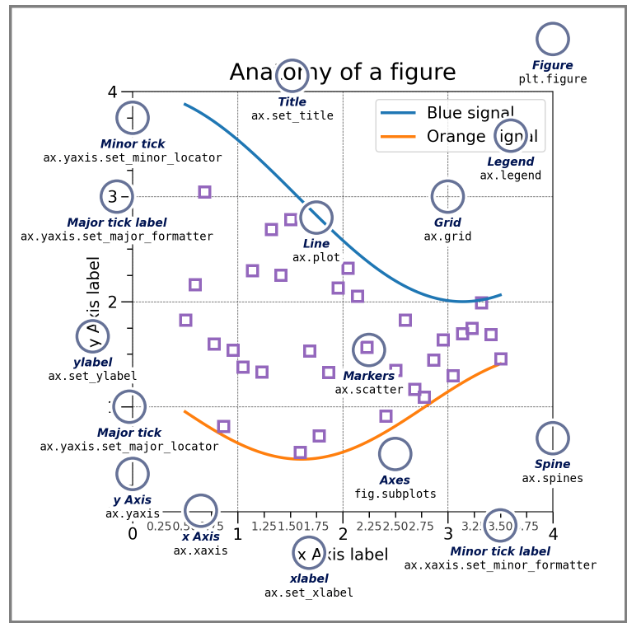
\includegraphics{./imgs/unidad_6/matplotlib.png}

}

\caption{Partes de una Figura}

\end{figure}%

Si desea conocer más detalle, puede ingresar a
\url{https://matplotlib.org/stable/tutorials/introductory/quick_start.html}.

Con lo aprendido hasta el momento, vamos a realizar nuestro primer
gráfico para luego mostrar cómo modificar su aspecto. La función que
usaremos es \texttt{plot()}, con la que se obteniene un gráfico de
línea; esta recibe los vectores X e Y para formar puntos en el plano
cartesiano que son unidos con una línea.

\begin{Shaded}
\begin{Highlighting}[]
\CommentTok{\# Grafico elemental}
\NormalTok{x }\OperatorTok{=}\NormalTok{ [}\DecValTok{0}\NormalTok{,}\DecValTok{2}\NormalTok{,}\DecValTok{10}\NormalTok{,}\DecValTok{11}\NormalTok{,}\DecValTok{18}\NormalTok{,}\DecValTok{25}\NormalTok{]}
\NormalTok{y }\OperatorTok{=}\NormalTok{ [}\DecValTok{0}\NormalTok{,}\DecValTok{1}\NormalTok{,}\DecValTok{2}\NormalTok{,}\DecValTok{3}\NormalTok{,}\DecValTok{4}\NormalTok{,}\DecValTok{5}\NormalTok{]}

\NormalTok{fig, ax }\OperatorTok{=}\NormalTok{ plt.subplots()}

\CommentTok{\# Gráfico de línea}
\NormalTok{ax.plot(x, y)}
\NormalTok{plt.show()}
\end{Highlighting}
\end{Shaded}

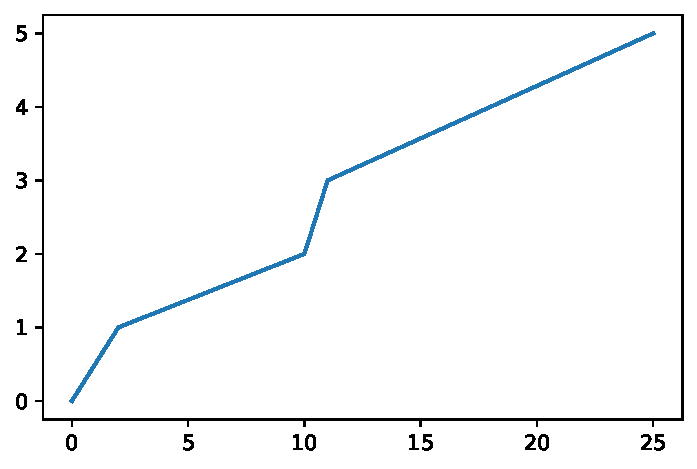
\includegraphics{unidad_6_files/figure-pdf/cell-110-output-1.pdf}

\subsubsection{Cambiar el aspecto de los
gráficos:}\label{cambiar-el-aspecto-de-los-gruxe1ficos}

Para diferenciar las curvas o simplemente para modificar los gráficos
según nuestros gustos personales, se pueden definir los distintos
parámetros dentro de \texttt{plot()}, estableciendo el tipo de línea y
puntos, el grosor, el color, etc:

\begin{itemize}
\tightlist
\item
  \textbf{color =} nombre del color, por ejemplo:
  \texttt{\textquotesingle{}blue\textquotesingle{},\ \textquotesingle{}green\textquotesingle{},\ \textquotesingle{}red\textquotesingle{}},
  etc.
\item
  \textbf{marker =} forma de los puntos o marcadores, por ejemplo:
  \texttt{\textquotesingle{}\^{}\textquotesingle{},\ \textquotesingle{}o\textquotesingle{},\ \textquotesingle{}v\textquotesingle{}},
  etc.
\item
  \textbf{linestyle =} estilo de línea, por ejemplo:
  \texttt{\textquotesingle{}solid\textquotesingle{},\ \textquotesingle{}dashed\textquotesingle{},\ \textquotesingle{}dotted\textquotesingle{}}
  o sus
  equivalentes:\texttt{\textquotesingle{}-\textquotesingle{},\ \textquotesingle{}-\/-\textquotesingle{},\ \textquotesingle{}:\textquotesingle{},}
  entre otros.
\item
  \textbf{markersize, linewidth =} con un número, establecemos el tamaño
  del marcador y el espesor de la línea respectivamente.
\end{itemize}

Note que si no le asignamos un valor, se establecen los predefinidos.

\begin{Shaded}
\begin{Highlighting}[]
\NormalTok{x }\OperatorTok{=}\NormalTok{ [}\DecValTok{0}\NormalTok{,}\DecValTok{2}\NormalTok{,}\DecValTok{10}\NormalTok{,}\DecValTok{11}\NormalTok{,}\DecValTok{18}\NormalTok{,}\DecValTok{25}\NormalTok{]   }\CommentTok{\# Tiempo (min)}
\NormalTok{y }\OperatorTok{=}\NormalTok{ [}\DecValTok{0}\NormalTok{,}\DecValTok{1}\NormalTok{,}\DecValTok{2}\NormalTok{,}\DecValTok{3}\NormalTok{,}\DecValTok{4}\NormalTok{,}\DecValTok{5}\NormalTok{]       }\CommentTok{\# Distancia (m)}

\NormalTok{fig, ax }\OperatorTok{=}\NormalTok{ plt.subplots()}

\NormalTok{ax.plot(x, y, color}\OperatorTok{=}\StringTok{\textquotesingle{}green\textquotesingle{}}\NormalTok{, marker}\OperatorTok{=}\StringTok{\textquotesingle{}\^{}\textquotesingle{}}\NormalTok{, linestyle}\OperatorTok{=}\StringTok{\textquotesingle{}{-}{-}\textquotesingle{}}\NormalTok{, markersize}\OperatorTok{=}\DecValTok{8}\NormalTok{, linewidth}\OperatorTok{=}\FloatTok{1.2}\NormalTok{)}
\NormalTok{plt.show()}
\end{Highlighting}
\end{Shaded}

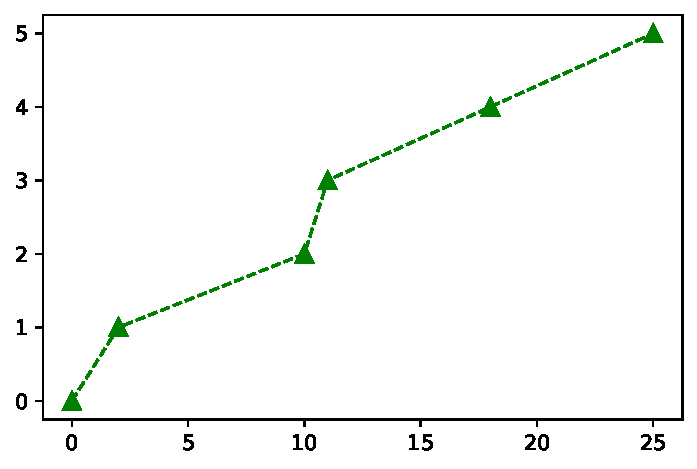
\includegraphics{unidad_6_files/figure-pdf/cell-111-output-1.pdf}

Para ver las múltiples opciones disponibles, les dejamos el siguiente
link de consulta:
\url{https://matplotlib.org/2.1.1/api/_as_gen/matplotlib.pyplot.plot.html}

\subsubsection{Grilla o cuadrícula:}\label{grilla-o-cuadruxedcula}

Para leer facilmente el valor de cada punto, podemos agregar una
cuadrícula usando \texttt{grid()}.

Si deseamos modificarle, por ejemplo, el color, el estilo de línea, o
sólo queremos ver uno de los ejes, podemos indicarlo utilizando
parámetros muy similares a los vistos anteriormente pero en la funcion
\texttt{grid()}.

\begin{Shaded}
\begin{Highlighting}[]
\NormalTok{x }\OperatorTok{=}\NormalTok{ [}\DecValTok{0}\NormalTok{,}\DecValTok{2}\NormalTok{,}\DecValTok{10}\NormalTok{,}\DecValTok{11}\NormalTok{,}\DecValTok{18}\NormalTok{,}\DecValTok{25}\NormalTok{]   }\CommentTok{\# Tiempo (min)}
\NormalTok{y }\OperatorTok{=}\NormalTok{ [}\DecValTok{0}\NormalTok{,}\DecValTok{1}\NormalTok{,}\DecValTok{2}\NormalTok{,}\DecValTok{3}\NormalTok{,}\DecValTok{4}\NormalTok{,}\DecValTok{5}\NormalTok{]       }\CommentTok{\# Distancia (m)}

\NormalTok{fig, ax }\OperatorTok{=}\NormalTok{ plt.subplots()}

\NormalTok{ax.plot(x, y, color}\OperatorTok{=}\StringTok{\textquotesingle{}green\textquotesingle{}}\NormalTok{, marker}\OperatorTok{=}\StringTok{\textquotesingle{}\^{}\textquotesingle{}}\NormalTok{, linestyle}\OperatorTok{=}\StringTok{\textquotesingle{}{-}{-}\textquotesingle{}}\NormalTok{, markersize}\OperatorTok{=}\DecValTok{8}\NormalTok{, linewidth}\OperatorTok{=}\FloatTok{1.2}\NormalTok{)}

\CommentTok{\# Grilla preestablecida}
\NormalTok{ax.grid()}
\NormalTok{plt.show()}
\end{Highlighting}
\end{Shaded}

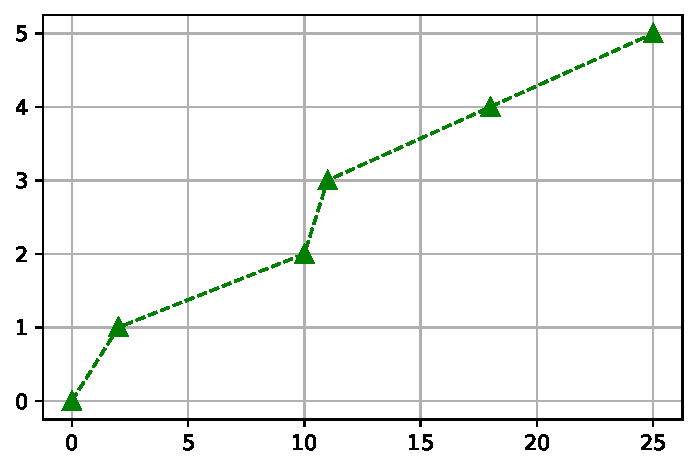
\includegraphics{unidad_6_files/figure-pdf/cell-112-output-1.pdf}

\begin{Shaded}
\begin{Highlighting}[]
\CommentTok{\#Gráfica con la grilla preestablecida}
\NormalTok{x }\OperatorTok{=}\NormalTok{ [}\DecValTok{0}\NormalTok{,}\DecValTok{2}\NormalTok{,}\DecValTok{10}\NormalTok{,}\DecValTok{11}\NormalTok{,}\DecValTok{18}\NormalTok{,}\DecValTok{25}\NormalTok{]   }\CommentTok{\# Tiempo (min)}
\NormalTok{y }\OperatorTok{=}\NormalTok{ [}\DecValTok{0}\NormalTok{,}\DecValTok{1}\NormalTok{,}\DecValTok{2}\NormalTok{,}\DecValTok{3}\NormalTok{,}\DecValTok{4}\NormalTok{,}\DecValTok{5}\NormalTok{]       }\CommentTok{\# Distancia (m)}

\NormalTok{fig, ax }\OperatorTok{=}\NormalTok{ plt.subplots()}

\NormalTok{ax.plot(x, y, color}\OperatorTok{=}\StringTok{\textquotesingle{}green\textquotesingle{}}\NormalTok{, marker}\OperatorTok{=}\StringTok{\textquotesingle{}\^{}\textquotesingle{}}\NormalTok{, linestyle}\OperatorTok{=}\StringTok{\textquotesingle{}{-}{-}\textquotesingle{}}\NormalTok{, markersize}\OperatorTok{=}\DecValTok{8}\NormalTok{, linewidth}\OperatorTok{=}\FloatTok{1.2}\NormalTok{)}

\CommentTok{\#Grilla modificada}
\NormalTok{ax.grid(axis }\OperatorTok{=} \StringTok{\textquotesingle{}y\textquotesingle{}}\NormalTok{, color }\OperatorTok{=} \StringTok{\textquotesingle{}gray\textquotesingle{}}\NormalTok{, linestyle }\OperatorTok{=} \StringTok{\textquotesingle{}dashed\textquotesingle{}}\NormalTok{)}
\NormalTok{plt.show()}
\end{Highlighting}
\end{Shaded}

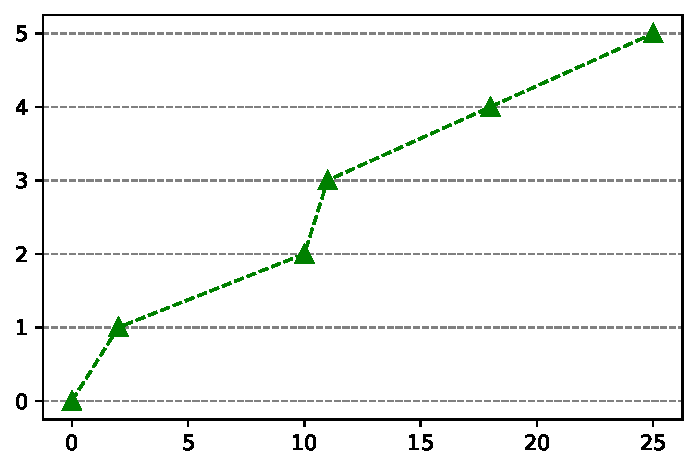
\includegraphics{unidad_6_files/figure-pdf/cell-113-output-1.pdf}

\subsubsection{Títulos}\label{tuxedtulos}

Una de las partes más importantes para que un gráfico se pueda entender
es ponerle un título y explicar qué significa cada eje. Eso se hace con
las funciones \texttt{set\_xlabel()}, \texttt{set\_ylabel()} y
\texttt{set\_title()}. Cada una recibe un string que se usará como
etiqueta del eje X, etiqueta del eje Y o título, respectivamente.

Siendo que los valores de \textbf{x} son el tiempo medido en minutos y
los de \textbf{y} una distancia en metros, entonces:

\begin{Shaded}
\begin{Highlighting}[]
\NormalTok{x }\OperatorTok{=}\NormalTok{ [}\DecValTok{0}\NormalTok{,}\DecValTok{2}\NormalTok{,}\DecValTok{10}\NormalTok{,}\DecValTok{11}\NormalTok{,}\DecValTok{18}\NormalTok{,}\DecValTok{25}\NormalTok{]   }\CommentTok{\# Tiempo (min)}
\NormalTok{y }\OperatorTok{=}\NormalTok{ [}\DecValTok{0}\NormalTok{,}\DecValTok{1}\NormalTok{,}\DecValTok{2}\NormalTok{,}\DecValTok{3}\NormalTok{,}\DecValTok{4}\NormalTok{,}\DecValTok{5}\NormalTok{]       }\CommentTok{\# Distancia (m)}

\NormalTok{fig, ax }\OperatorTok{=}\NormalTok{ plt.subplots()}

\NormalTok{ax.plot(x, y, color}\OperatorTok{=}\StringTok{\textquotesingle{}green\textquotesingle{}}\NormalTok{, marker}\OperatorTok{=}\StringTok{\textquotesingle{}\^{}\textquotesingle{}}\NormalTok{, linestyle}\OperatorTok{=}\StringTok{\textquotesingle{}{-}{-}\textquotesingle{}}\NormalTok{, markersize}\OperatorTok{=}\DecValTok{8}\NormalTok{, linewidth}\OperatorTok{=}\FloatTok{1.2}\NormalTok{)}

\CommentTok{\# Mostrar el título del gráfico}
\NormalTok{ax.set\_title(}\StringTok{"Gráfico de posición"}\NormalTok{)}

\CommentTok{\# Mostrar el título de los ejes}
\NormalTok{ax.set\_xlabel(}\StringTok{\textquotesingle{}Tiempo (min)\textquotesingle{}}\NormalTok{)}
\NormalTok{ax.set\_ylabel(}\StringTok{\textquotesingle{}Distancia (m)\textquotesingle{}}\NormalTok{)}

\CommentTok{\# Grilla preestablecida}
\NormalTok{ax.grid()}
\NormalTok{plt.show()}
\end{Highlighting}
\end{Shaded}

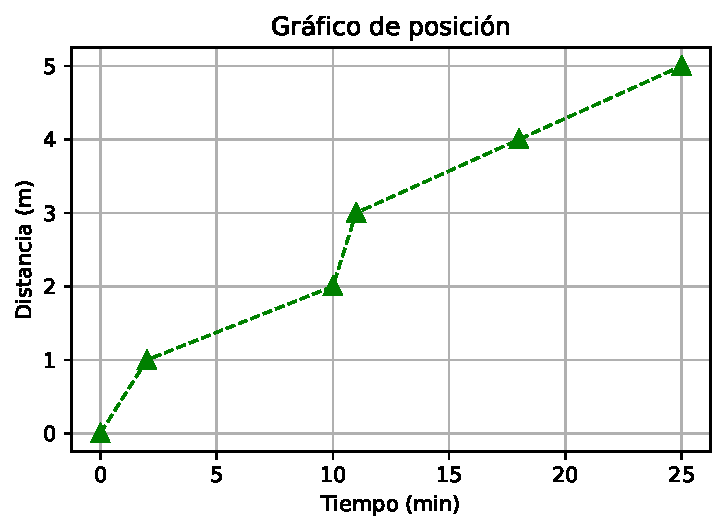
\includegraphics{unidad_6_files/figure-pdf/cell-114-output-1.pdf}

\subsubsection{Referencias}\label{referencias}

El gráfico con el que estamos trabajando sólo tiene una línea, pero si
contara con más de una, el uso de referencias sería escencial para
lograr el entendimiento del mismo. Para rotular las líneas, dentro de
\texttt{plot()} se debe definir la referencia como \texttt{label}. Luego
se coloca \texttt{legend()}

\begin{Shaded}
\begin{Highlighting}[]
\NormalTok{x }\OperatorTok{=}\NormalTok{ [}\DecValTok{0}\NormalTok{,}\DecValTok{2}\NormalTok{,}\DecValTok{10}\NormalTok{,}\DecValTok{11}\NormalTok{,}\DecValTok{18}\NormalTok{,}\DecValTok{25}\NormalTok{]   }\CommentTok{\# Tiempo (min)}
\NormalTok{y }\OperatorTok{=}\NormalTok{ [}\DecValTok{0}\NormalTok{,}\DecValTok{1}\NormalTok{,}\DecValTok{2}\NormalTok{,}\DecValTok{3}\NormalTok{,}\DecValTok{4}\NormalTok{,}\DecValTok{5}\NormalTok{]       }\CommentTok{\# Distancia (m)}

\NormalTok{fig, ax }\OperatorTok{=}\NormalTok{ plt.subplots()}

\NormalTok{ax.plot(x, y, label}\OperatorTok{=}\StringTok{\textquotesingle{}Objeto 1\textquotesingle{}}\NormalTok{, color}\OperatorTok{=}\StringTok{\textquotesingle{}green\textquotesingle{}}\NormalTok{, marker}\OperatorTok{=}\StringTok{\textquotesingle{}\^{}\textquotesingle{}}\NormalTok{, linestyle}\OperatorTok{=}\StringTok{\textquotesingle{}{-}{-}\textquotesingle{}}\NormalTok{, markersize}\OperatorTok{=}\DecValTok{8}\NormalTok{, linewidth}\OperatorTok{=}\FloatTok{1.2}\NormalTok{)}

\CommentTok{\# Mostrar el título del gráfico}
\NormalTok{ax.set\_title(}\StringTok{"Gráfico de posición"}\NormalTok{)}

\CommentTok{\# Mostrar el título de los ejes}
\NormalTok{ax.set\_xlabel(}\StringTok{\textquotesingle{}Tiempo (min)\textquotesingle{}}\NormalTok{)}
\NormalTok{ax.set\_ylabel(}\StringTok{\textquotesingle{}Distancia (m)\textquotesingle{}}\NormalTok{)}

\CommentTok{\# Agregar la refencia}
\NormalTok{ax.legend()}

\CommentTok{\# Grilla preestablecida}
\NormalTok{ax.grid()}
\NormalTok{plt.show()}
\end{Highlighting}
\end{Shaded}

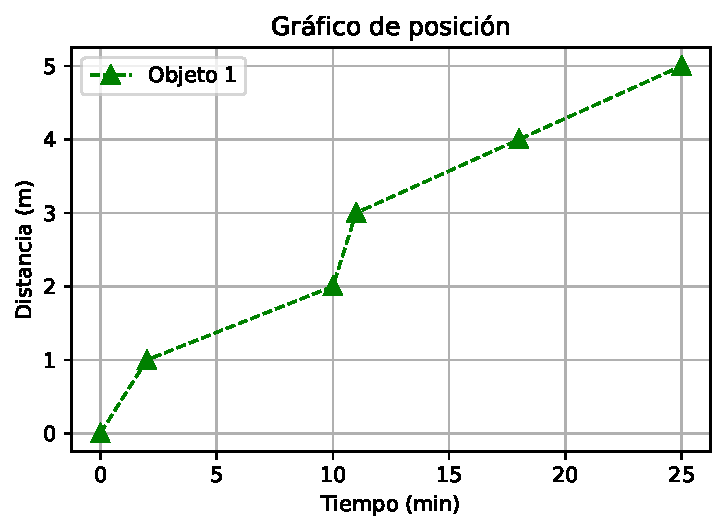
\includegraphics{unidad_6_files/figure-pdf/cell-115-output-1.pdf}

\subsubsection{Características de los
ejes:}\label{caracteruxedsticas-de-los-ejes}

Como podemos identificar en los gráficos anteriores, Python decidió las
características de los ejes:

\begin{itemize}
\tightlist
\item
  \textbf{Eje x}: se extiende del 0 a 25, de 5 en 5.
\item
  \textbf{Eje y}: se extiende del 0 a 5, de 1 en 1.
\end{itemize}

Podemos establecer los limites del eje x e y usando \texttt{set\_xlim()}
y \texttt{set\_ylim()} respectivamente.

\begin{Shaded}
\begin{Highlighting}[]
\NormalTok{x }\OperatorTok{=}\NormalTok{ [}\DecValTok{0}\NormalTok{,}\DecValTok{2}\NormalTok{,}\DecValTok{10}\NormalTok{,}\DecValTok{11}\NormalTok{,}\DecValTok{18}\NormalTok{,}\DecValTok{25}\NormalTok{]   }\CommentTok{\# Tiempo (min)}
\NormalTok{y }\OperatorTok{=}\NormalTok{ [}\DecValTok{0}\NormalTok{,}\DecValTok{1}\NormalTok{,}\DecValTok{2}\NormalTok{,}\DecValTok{3}\NormalTok{,}\DecValTok{4}\NormalTok{,}\DecValTok{5}\NormalTok{]       }\CommentTok{\# Distancia (m)}

\NormalTok{fig, ax }\OperatorTok{=}\NormalTok{ plt.subplots()}

\NormalTok{ax.plot(x, y, label}\OperatorTok{=}\StringTok{\textquotesingle{}Objeto 1\textquotesingle{}}\NormalTok{, color}\OperatorTok{=}\StringTok{\textquotesingle{}green\textquotesingle{}}\NormalTok{, marker}\OperatorTok{=}\StringTok{\textquotesingle{}\^{}\textquotesingle{}}\NormalTok{, linestyle}\OperatorTok{=}\StringTok{\textquotesingle{}{-}{-}\textquotesingle{}}\NormalTok{,}
\NormalTok{        markersize}\OperatorTok{=}\DecValTok{8}\NormalTok{, linewidth}\OperatorTok{=}\FloatTok{1.2}\NormalTok{)}

\CommentTok{\# Mostrar el título del gráfico}
\NormalTok{ax.set\_title(}\StringTok{"Gráfico de posición"}\NormalTok{)}

\CommentTok{\# Mostrar el título de los ejes}
\NormalTok{ax.set\_xlabel(}\StringTok{\textquotesingle{}Tiempo (min)\textquotesingle{}}\NormalTok{)}
\NormalTok{ax.set\_ylabel(}\StringTok{\textquotesingle{}Distancia (m)\textquotesingle{}}\NormalTok{)}

\CommentTok{\# Establecer los límites de los ejes}
\NormalTok{ax.set\_xlim(}\DecValTok{0}\NormalTok{, }\DecValTok{30}\NormalTok{)}
\NormalTok{ax.set\_ylim(}\DecValTok{0}\NormalTok{, }\DecValTok{6}\NormalTok{)}

\CommentTok{\# Agregar la refencia}
\NormalTok{ax.legend()}

\CommentTok{\# Grilla preestablecida}
\NormalTok{ax.grid()}
\NormalTok{plt.show()}
\end{Highlighting}
\end{Shaded}

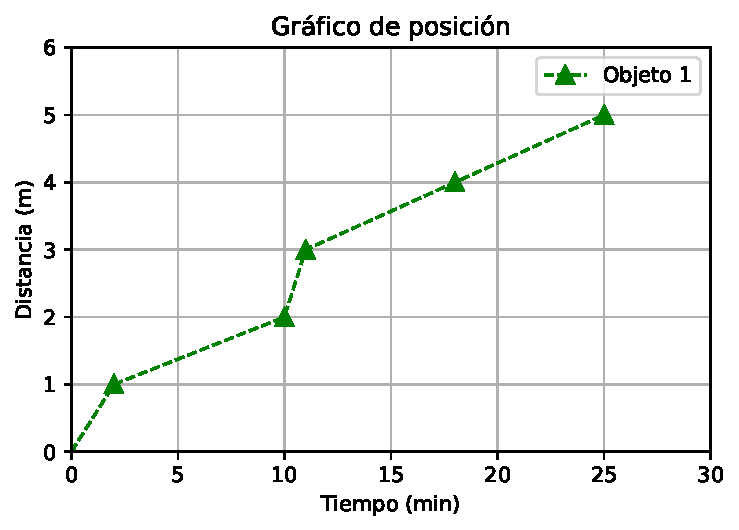
\includegraphics{unidad_6_files/figure-pdf/cell-116-output-1.pdf}

\subsection{Tipos de gráficos}\label{tipos-de-gruxe1ficos}

A continuación, vamos a ver ejemplos de los tipos de gráficos más
comunes, las funciones que son necesarias para crearlos y cuándo se debe
utilizar cada uno de ellos.

Para estos ejemplos, los datos a graficar son valores de listas
únicamente por fines didácticos, ya que podría tratarse de arrays o
columnas de DataFrames. Además, recuerden que mucho de lo aprendido para
modificar el aspecto de un gráfico, como agregar títulos, cuadrículas,
límites a los ejes, etc., se puede aplicar también en estas figuras.:

\subsubsection{Gráfico de línea}\label{gruxe1fico-de-luxednea}

El gráfico de línea permite visualizar cambios en los valores lo largo
de un rango continuo (tendencias), como puede ser el tiempo o la
distancia. Para crearlo, se utiliza la función \texttt{plot()}, como
vimos anteriormente:

\begin{Shaded}
\begin{Highlighting}[]
\NormalTok{x }\OperatorTok{=}\NormalTok{ [}\DecValTok{0}\NormalTok{,}\DecValTok{2}\NormalTok{,}\DecValTok{10}\NormalTok{,}\DecValTok{11}\NormalTok{,}\DecValTok{18}\NormalTok{,}\DecValTok{25}\NormalTok{]}
\NormalTok{y }\OperatorTok{=}\NormalTok{ [}\DecValTok{0}\NormalTok{,}\DecValTok{1}\NormalTok{,}\DecValTok{2}\NormalTok{,}\DecValTok{3}\NormalTok{,}\DecValTok{4}\NormalTok{,}\DecValTok{5}\NormalTok{]}

\NormalTok{fig, ax }\OperatorTok{=}\NormalTok{ plt.subplots()}

\NormalTok{ax.plot(x, y)}
\NormalTok{plt.show()}
\end{Highlighting}
\end{Shaded}

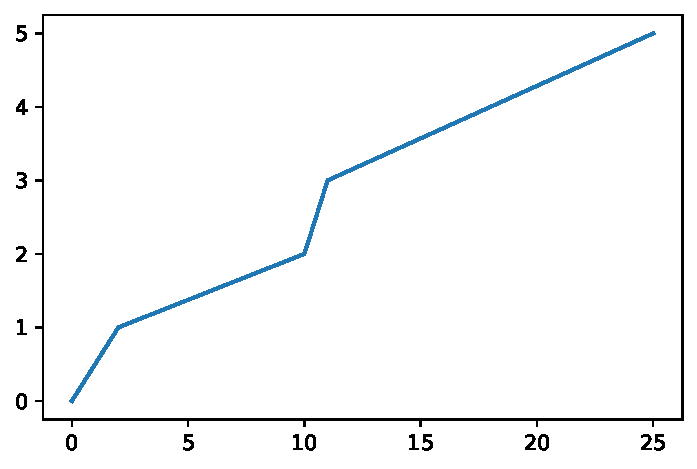
\includegraphics{unidad_6_files/figure-pdf/cell-117-output-1.pdf}

\subsubsection{Gráfico de dispersión o
puntos}\label{gruxe1fico-de-dispersiuxf3n-o-puntos}

El gráfico de dispersión o puntos permite visualizar la relación entre
las variables. Para crearlo, se utiliza la función \texttt{scatter()}:

\begin{Shaded}
\begin{Highlighting}[]
\NormalTok{x }\OperatorTok{=}\NormalTok{ [}\DecValTok{5}\NormalTok{,}\DecValTok{7}\NormalTok{,}\DecValTok{8}\NormalTok{,}\DecValTok{7}\NormalTok{,}\DecValTok{2}\NormalTok{,}\DecValTok{17}\NormalTok{,}\DecValTok{2}\NormalTok{,}\DecValTok{9}\NormalTok{,}\DecValTok{4}\NormalTok{,}\DecValTok{11}\NormalTok{,}\DecValTok{12}\NormalTok{,}\DecValTok{9}\NormalTok{,}\DecValTok{6}\NormalTok{]}
\NormalTok{y }\OperatorTok{=}\NormalTok{ [}\DecValTok{99}\NormalTok{,}\DecValTok{86}\NormalTok{,}\DecValTok{87}\NormalTok{,}\DecValTok{88}\NormalTok{,}\DecValTok{111}\NormalTok{,}\DecValTok{86}\NormalTok{,}\DecValTok{103}\NormalTok{,}\DecValTok{87}\NormalTok{,}\DecValTok{94}\NormalTok{,}\DecValTok{78}\NormalTok{,}\DecValTok{77}\NormalTok{,}\DecValTok{85}\NormalTok{,}\DecValTok{86}\NormalTok{]}

\NormalTok{fig, ax }\OperatorTok{=}\NormalTok{ plt.subplots()}

\NormalTok{ax.scatter(x, y)}
\NormalTok{plt.show()}
\end{Highlighting}
\end{Shaded}

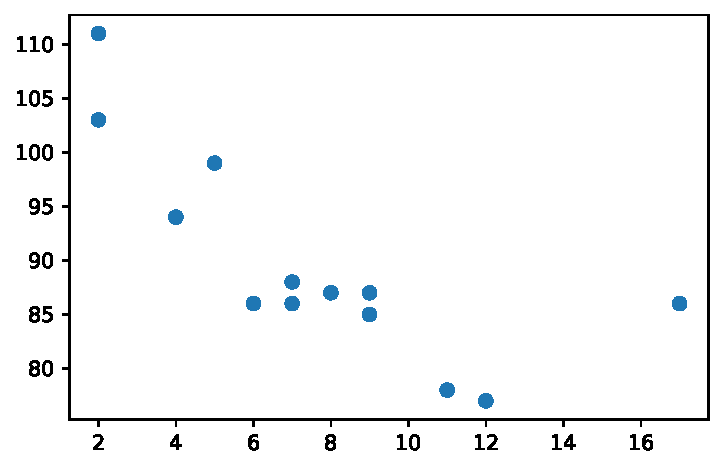
\includegraphics{unidad_6_files/figure-pdf/cell-118-output-1.pdf}

\subsubsection{Gráfico de barras}\label{gruxe1fico-de-barras}

El gráfico de barras permite visualizar proporciones, comparando dos o
más valores entre sí. Para crearlo, se utiliza la función
\texttt{bar()}, la cual primero recibe, en primer lugar, las etiquetas
de las barras que se van a mostrar y en segundo lugar, la altura
correspondiente a cada una de estas barras.

\begin{Shaded}
\begin{Highlighting}[]
\NormalTok{peso }\OperatorTok{=}\NormalTok{ [}\DecValTok{340}\NormalTok{, }\DecValTok{115}\NormalTok{, }\DecValTok{200}\NormalTok{, }\DecValTok{200}\NormalTok{, }\DecValTok{270}\NormalTok{]}
\NormalTok{ingredientes }\OperatorTok{=}\NormalTok{ [}\StringTok{\textquotesingle{}chocolate\textquotesingle{}}\NormalTok{, }\StringTok{\textquotesingle{}manteca\textquotesingle{}}\NormalTok{, }\StringTok{\textquotesingle{}azúcar\textquotesingle{}}\NormalTok{, }\StringTok{\textquotesingle{}huevo\textquotesingle{}}\NormalTok{, }\StringTok{\textquotesingle{}harina\textquotesingle{}}\NormalTok{]}

\NormalTok{fig, ax }\OperatorTok{=}\NormalTok{ plt.subplots()}

\NormalTok{ax.bar(ingredientes, peso)}

\NormalTok{ax.set\_xlabel(}\StringTok{\textquotesingle{}Ingredientes\textquotesingle{}}\NormalTok{)}
\NormalTok{ax.set\_ylabel(}\StringTok{\textquotesingle{}Masa (g)\textquotesingle{}}\NormalTok{)}

\NormalTok{ax.set\_title(}\StringTok{"Receta"}\NormalTok{)}

\NormalTok{plt.show()}
\end{Highlighting}
\end{Shaded}

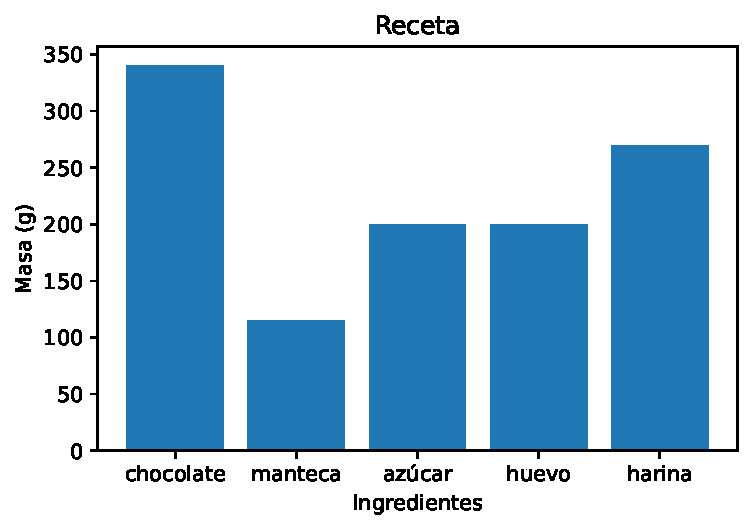
\includegraphics{unidad_6_files/figure-pdf/cell-119-output-1.pdf}

Note que con la función anterior, las barras adquieren una dirección
vertical: si quisieramos verlas de manera horizontal, debemos usar la
función \texttt{barh()} y cambiar los títulos de los ejes según
corresponda:

\begin{Shaded}
\begin{Highlighting}[]
\NormalTok{peso }\OperatorTok{=}\NormalTok{ [}\DecValTok{340}\NormalTok{, }\DecValTok{115}\NormalTok{, }\DecValTok{200}\NormalTok{, }\DecValTok{200}\NormalTok{, }\DecValTok{270}\NormalTok{]}
\NormalTok{ingredientes }\OperatorTok{=}\NormalTok{ [}\StringTok{\textquotesingle{}chocolate\textquotesingle{}}\NormalTok{, }\StringTok{\textquotesingle{}manteca\textquotesingle{}}\NormalTok{, }\StringTok{\textquotesingle{}azúcar\textquotesingle{}}\NormalTok{, }\StringTok{\textquotesingle{}huevo\textquotesingle{}}\NormalTok{, }\StringTok{\textquotesingle{}harina\textquotesingle{}}\NormalTok{]}

\NormalTok{fig, ax }\OperatorTok{=}\NormalTok{ plt.subplots()}

\NormalTok{ax.barh(ingredientes, peso)}

\NormalTok{ax.set\_ylabel(}\StringTok{\textquotesingle{}Ingredientes\textquotesingle{}}\NormalTok{)}
\NormalTok{ax.set\_xlabel(}\StringTok{\textquotesingle{}Masa (g)\textquotesingle{}}\NormalTok{)}

\NormalTok{ax.set\_title(}\StringTok{"Receta"}\NormalTok{)}

\NormalTok{plt.show()}
\end{Highlighting}
\end{Shaded}

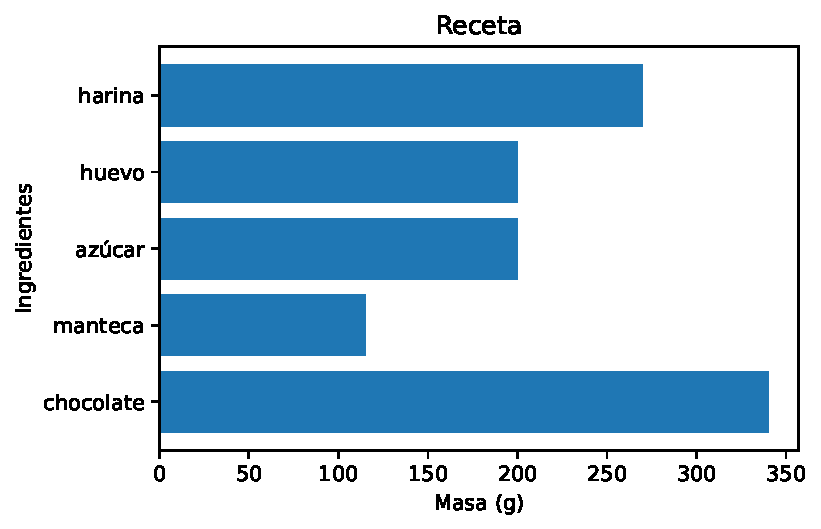
\includegraphics{unidad_6_files/figure-pdf/cell-120-output-1.pdf}

\subsubsection{Gráfico de torta}\label{gruxe1fico-de-torta}

El gráfico de torta, como el de barras, permite visualizar y comparar
proporciones pero de manera circular y como partes de un todo. Para
crearlo, se utiliza la función \texttt{pie()}, la cual podría recibir
solamente números pero es útil también saber qué simboliza cada parte.
Por eso, para referenciar cada porción se usa el parámetro
\texttt{labels}. Por otro lado, el parámetro \texttt{autopct} establece
cómo se mostrará el porcentaje: por ejemplo, \texttt{\%1.1f\%\%} le
indica que el porcentaje tendrá un decimal, mientras que
\texttt{\%1.2f\%\%} tendrá dos decimales.

\begin{Shaded}
\begin{Highlighting}[]
\NormalTok{peso }\OperatorTok{=}\NormalTok{ [}\DecValTok{340}\NormalTok{, }\DecValTok{115}\NormalTok{, }\DecValTok{200}\NormalTok{, }\DecValTok{200}\NormalTok{, }\DecValTok{270}\NormalTok{]}
\NormalTok{ingredientes }\OperatorTok{=}\NormalTok{ [}\StringTok{\textquotesingle{}chocolate\textquotesingle{}}\NormalTok{, }\StringTok{\textquotesingle{}manteca\textquotesingle{}}\NormalTok{, }\StringTok{\textquotesingle{}azúcar\textquotesingle{}}\NormalTok{, }\StringTok{\textquotesingle{}huevo\textquotesingle{}}\NormalTok{, }\StringTok{\textquotesingle{}harina\textquotesingle{}}\NormalTok{]}

\NormalTok{fig, ax }\OperatorTok{=}\NormalTok{ plt.subplots()}

\NormalTok{ax.pie(peso, labels}\OperatorTok{=}\NormalTok{ ingredientes, autopct}\OperatorTok{=}\StringTok{\textquotesingle{}}\SpecialCharTok{\%1.1f\%\%}\StringTok{\textquotesingle{}}\NormalTok{)}

\NormalTok{ax.set\_title(}\StringTok{"Receta"}\NormalTok{)}

\NormalTok{plt.show()}
\end{Highlighting}
\end{Shaded}

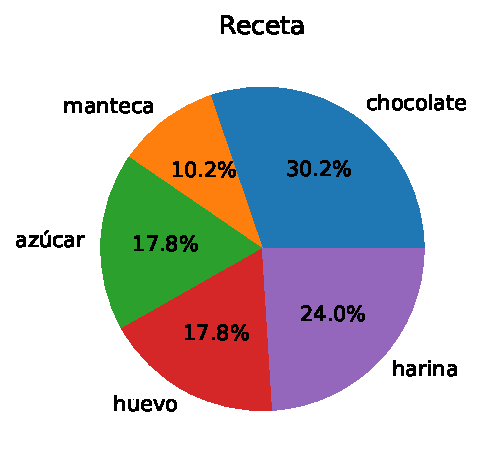
\includegraphics{unidad_6_files/figure-pdf/cell-121-output-1.pdf}

\subsection{Gráficos múltiples}\label{gruxe1ficos-muxfaltiples}

En los casos anteriores, creamos siempre un sólo gráfico con una curva,
en una figura. Pero\ldots{} \textbf{¿Cómo podríamos graficar varias
curvas en un mismo gráfico?}

\begin{Shaded}
\begin{Highlighting}[]
\CommentTok{\# Valores que se desean graficar}
\NormalTok{x }\OperatorTok{=}\NormalTok{ [}\DecValTok{0}\NormalTok{, }\DecValTok{1}\NormalTok{, }\DecValTok{2}\NormalTok{, }\DecValTok{3}\NormalTok{, }\DecValTok{4}\NormalTok{, }\DecValTok{5}\NormalTok{]}
\NormalTok{y\_linear }\OperatorTok{=}\NormalTok{ [}\DecValTok{0}\NormalTok{, }\DecValTok{1}\NormalTok{, }\DecValTok{2}\NormalTok{, }\DecValTok{3}\NormalTok{, }\DecValTok{4}\NormalTok{, }\DecValTok{5}\NormalTok{]}
\NormalTok{y\_quadratic }\OperatorTok{=}\NormalTok{ [}\DecValTok{0}\NormalTok{, }\DecValTok{1}\NormalTok{, }\DecValTok{4}\NormalTok{, }\DecValTok{9}\NormalTok{, }\DecValTok{16}\NormalTok{, }\DecValTok{25}\NormalTok{]}
\NormalTok{y\_cubic }\OperatorTok{=}\NormalTok{ [}\DecValTok{0}\NormalTok{, }\DecValTok{1}\NormalTok{, }\DecValTok{8}\NormalTok{, }\DecValTok{27}\NormalTok{, }\DecValTok{64}\NormalTok{, }\DecValTok{125}\NormalTok{]}

\NormalTok{fig, ax }\OperatorTok{=}\NormalTok{ plt.subplots(figsize}\OperatorTok{=}\NormalTok{(}\DecValTok{5}\NormalTok{, }\DecValTok{3}\NormalTok{))}

\NormalTok{ax.plot(x, y\_linear, label}\OperatorTok{=}\StringTok{\textquotesingle{}Lineal\textquotesingle{}}\NormalTok{)}
\NormalTok{ax.plot(x, y\_quadratic, label}\OperatorTok{=}\StringTok{\textquotesingle{}Cuadrático\textquotesingle{}}\NormalTok{)}
\NormalTok{ax.plot(x, y\_cubic, label}\OperatorTok{=}\StringTok{\textquotesingle{}Cúbico\textquotesingle{}}\NormalTok{)}

\NormalTok{ax.set\_title(}\StringTok{"Gráfico de múltiples curvas"}\NormalTok{)}
\NormalTok{ax.set\_xlabel(}\StringTok{\textquotesingle{}x\textquotesingle{}}\NormalTok{)}
\NormalTok{ax.set\_ylabel(}\StringTok{\textquotesingle{}y\textquotesingle{}}\NormalTok{)}
\NormalTok{ax.legend()}

\NormalTok{plt.show()}
\end{Highlighting}
\end{Shaded}

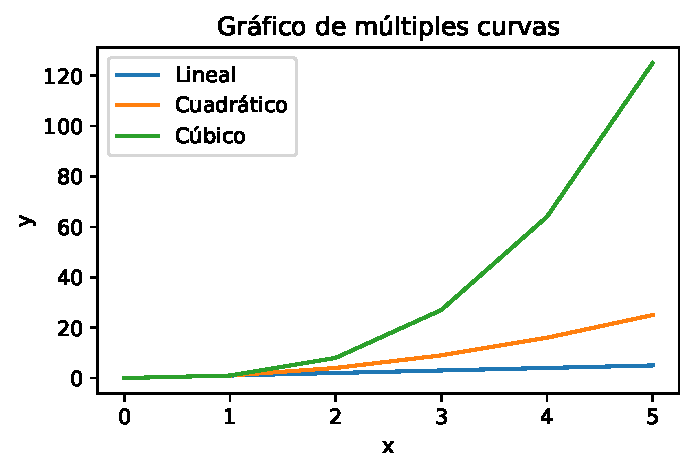
\includegraphics{unidad_6_files/figure-pdf/cell-122-output-1.pdf}

Note que se agregan nuevos datos al mismo axes, por lo que siempre
usamos \texttt{plot()} pero con distintos valores de \texttt{y}.
Asimismo, se estableció un tamaño de la figura con
\texttt{figsize=(width,\ height)}

\subsection{Grilla de gáficos}\label{grilla-de-guxe1ficos}

También podríamos querer ver varios axes en una misma figura. Para ello,
tenemos que definir, como si se tratase de una matriz o tabla, cuántas
columnas \texttt{ncols} y cuantas \texttt{nrows} de gráficos deseamos.
Por ejemplo, supongamos que quiero ver dos gráficos en una misma fila:

\begin{Shaded}
\begin{Highlighting}[]
\NormalTok{fig, ax }\OperatorTok{=}\NormalTok{ plt.subplots(nrows}\OperatorTok{=}\DecValTok{1}\NormalTok{, ncols}\OperatorTok{=}\DecValTok{2}\NormalTok{)   }\CommentTok{\# o simplemente plt.subplots(1,2)}
\end{Highlighting}
\end{Shaded}

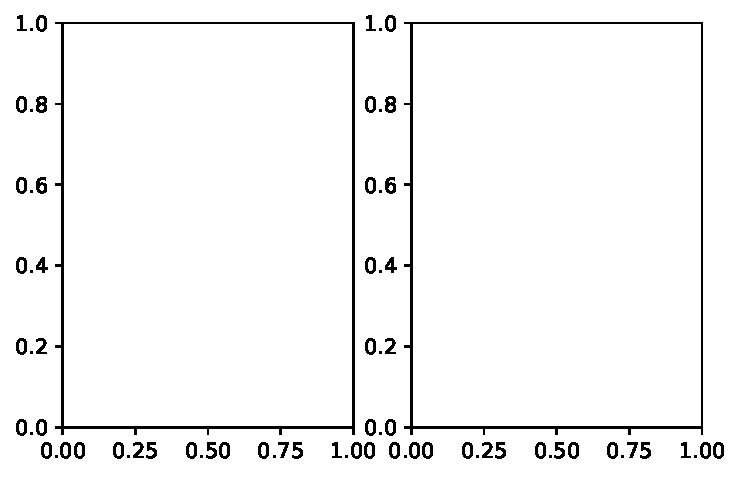
\includegraphics{unidad_6_files/figure-pdf/cell-123-output-1.pdf}

De manera análoga, podemos representar las 3 curvas anteriores pero
viendo 3 filas de gráficos en una única columna:

\begin{Shaded}
\begin{Highlighting}[]
\CommentTok{\# Valores que se desean graficar}
\NormalTok{x }\OperatorTok{=}\NormalTok{ [}\DecValTok{0}\NormalTok{, }\DecValTok{1}\NormalTok{, }\DecValTok{2}\NormalTok{, }\DecValTok{3}\NormalTok{, }\DecValTok{4}\NormalTok{, }\DecValTok{5}\NormalTok{]}
\NormalTok{x\_linear }\OperatorTok{=}\NormalTok{ [}\DecValTok{0}\NormalTok{, }\DecValTok{1}\NormalTok{, }\DecValTok{2}\NormalTok{, }\DecValTok{3}\NormalTok{, }\DecValTok{4}\NormalTok{, }\DecValTok{5}\NormalTok{]}
\NormalTok{x\_quadratic }\OperatorTok{=}\NormalTok{ [}\DecValTok{0}\NormalTok{, }\DecValTok{1}\NormalTok{, }\DecValTok{4}\NormalTok{, }\DecValTok{9}\NormalTok{, }\DecValTok{16}\NormalTok{, }\DecValTok{25}\NormalTok{]}
\NormalTok{x\_cubic }\OperatorTok{=}\NormalTok{ [}\DecValTok{0}\NormalTok{, }\DecValTok{1}\NormalTok{, }\DecValTok{8}\NormalTok{, }\DecValTok{27}\NormalTok{, }\DecValTok{64}\NormalTok{, }\DecValTok{125}\NormalTok{]}

\NormalTok{fig, ax }\OperatorTok{=}\NormalTok{ plt.subplots(nrows}\OperatorTok{=}\DecValTok{3}\NormalTok{, ncols}\OperatorTok{=}\DecValTok{1}\NormalTok{)}

\NormalTok{ax[}\DecValTok{0}\NormalTok{].plot(x, x\_linear)}
\NormalTok{ax[}\DecValTok{0}\NormalTok{].set\_title(}\StringTok{\textquotesingle{}Lineal\textquotesingle{}}\NormalTok{)}

\NormalTok{ax[}\DecValTok{1}\NormalTok{].plot(x, x\_quadratic)}
\NormalTok{ax[}\DecValTok{1}\NormalTok{].set\_title(}\StringTok{\textquotesingle{}Cuadrático\textquotesingle{}}\NormalTok{)}

\NormalTok{ax[}\DecValTok{2}\NormalTok{].plot(x, x\_cubic)}
\NormalTok{ax[}\DecValTok{2}\NormalTok{].set\_title(}\StringTok{\textquotesingle{}Cúbico\textquotesingle{}}\NormalTok{)}

\NormalTok{plt.show()}
\end{Highlighting}
\end{Shaded}

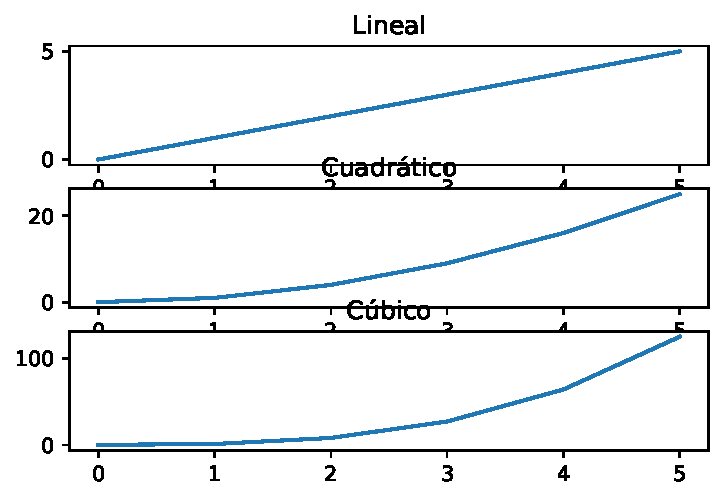
\includegraphics{unidad_6_files/figure-pdf/cell-124-output-1.pdf}

Entonces, lo único que debemos hacer es \textbf{indicar la posición del
axes con números dentro del corchete} . Si tengo varias columnas y
filas, dentro del corchete, se indica primero la fila y luego la
columna: \texttt{ax{[}fila,\ columna{]}}.

\begin{Shaded}
\begin{Highlighting}[]
\NormalTok{fig, ax }\OperatorTok{=}\NormalTok{ plt.subplots(nrows}\OperatorTok{=}\DecValTok{3}\NormalTok{, ncols}\OperatorTok{=}\DecValTok{3}\NormalTok{)}
\NormalTok{fig.subplots\_adjust(wspace}\OperatorTok{=}\FloatTok{0.5}\NormalTok{, hspace}\OperatorTok{=}\FloatTok{0.5}\NormalTok{) }\CommentTok{\# Con esto indicamos el espacio libre entre los subplots}

\NormalTok{ax[}\DecValTok{0}\NormalTok{, }\DecValTok{1}\NormalTok{].plot(x, x\_linear)}
\NormalTok{plt.show()}
\end{Highlighting}
\end{Shaded}

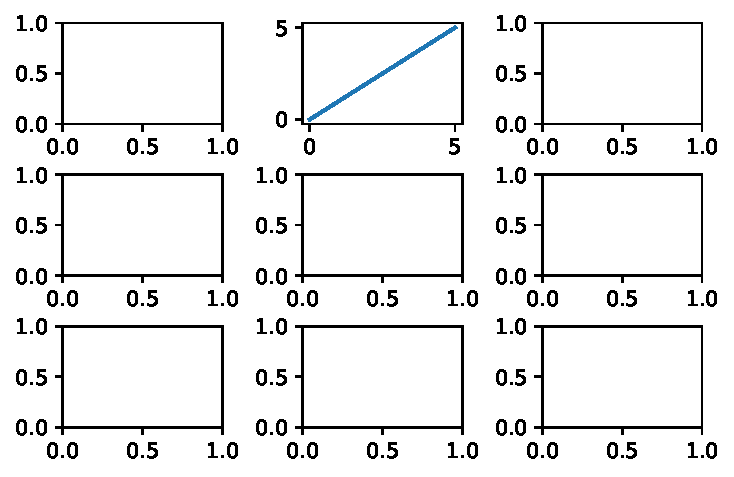
\includegraphics{unidad_6_files/figure-pdf/cell-125-output-1.pdf}

\subsection{Funciones de Gráficas}\label{funciones-de-gruxe1ficas}

En términos generales, si nos encontramos en la situacion de copiar y
pegar las mismas líneas de código para realizar gráficos similares,
trendríamos que pensar en crear una función que simplifique esta tarea.
Por ejemplo:

\begin{Shaded}
\begin{Highlighting}[]
\NormalTok{x }\OperatorTok{=}\NormalTok{ [}\DecValTok{0}\NormalTok{, }\DecValTok{1}\NormalTok{, }\DecValTok{2}\NormalTok{, }\DecValTok{3}\NormalTok{, }\DecValTok{4}\NormalTok{, }\DecValTok{5}\NormalTok{]}
\NormalTok{x\_linear }\OperatorTok{=}\NormalTok{ [}\DecValTok{0}\NormalTok{, }\DecValTok{1}\NormalTok{, }\DecValTok{2}\NormalTok{, }\DecValTok{3}\NormalTok{, }\DecValTok{4}\NormalTok{, }\DecValTok{5}\NormalTok{]}
\NormalTok{x\_quadratic }\OperatorTok{=}\NormalTok{ [}\DecValTok{0}\NormalTok{, }\DecValTok{1}\NormalTok{, }\DecValTok{4}\NormalTok{, }\DecValTok{9}\NormalTok{, }\DecValTok{16}\NormalTok{, }\DecValTok{25}\NormalTok{]}
\NormalTok{x\_cubic }\OperatorTok{=}\NormalTok{ [}\DecValTok{0}\NormalTok{, }\DecValTok{1}\NormalTok{, }\DecValTok{8}\NormalTok{, }\DecValTok{27}\NormalTok{, }\DecValTok{64}\NormalTok{, }\DecValTok{125}\NormalTok{]}

\NormalTok{fig, ax}\OperatorTok{=}\NormalTok{plt.subplots(}\DecValTok{3}\NormalTok{)}
\NormalTok{ax[}\DecValTok{0}\NormalTok{].plot(x,x\_linear,label}\OperatorTok{=}\StringTok{"$x$"}\NormalTok{,color}\OperatorTok{=}\StringTok{"r"}\NormalTok{)}
\NormalTok{ax[}\DecValTok{0}\NormalTok{].set\_xlabel(}\StringTok{"eje x"}\NormalTok{)}
\NormalTok{ax[}\DecValTok{0}\NormalTok{].set\_ylabel(}\StringTok{"eje y"}\NormalTok{)}
\NormalTok{ax[}\DecValTok{0}\NormalTok{].legend()}
\NormalTok{ax[}\DecValTok{0}\NormalTok{].grid()}


\NormalTok{ax[}\DecValTok{1}\NormalTok{].plot(x,x\_quadratic,label}\OperatorTok{=}\StringTok{"$x\^{}2$"}\NormalTok{,color}\OperatorTok{=}\StringTok{"b"}\NormalTok{)}
\NormalTok{ax[}\DecValTok{1}\NormalTok{].set\_xlabel(}\StringTok{"eje x"}\NormalTok{)}
\NormalTok{ax[}\DecValTok{1}\NormalTok{].set\_ylabel(}\StringTok{"eje y"}\NormalTok{)}
\NormalTok{ax[}\DecValTok{1}\NormalTok{].legend()}
\NormalTok{ax[}\DecValTok{1}\NormalTok{].grid()}


\NormalTok{ax[}\DecValTok{2}\NormalTok{].plot(x,x\_cubic,label}\OperatorTok{=}\StringTok{"$x\^{}3$"}\NormalTok{,color}\OperatorTok{=}\StringTok{"g"}\NormalTok{)}
\NormalTok{ax[}\DecValTok{2}\NormalTok{].set\_xlabel(}\StringTok{"eje x"}\NormalTok{)}
\NormalTok{ax[}\DecValTok{2}\NormalTok{].set\_ylabel(}\StringTok{"eje y"}\NormalTok{)}
\NormalTok{ax[}\DecValTok{2}\NormalTok{].legend()}
\NormalTok{ax[}\DecValTok{2}\NormalTok{].grid()}
\NormalTok{plt.show()}
\end{Highlighting}
\end{Shaded}

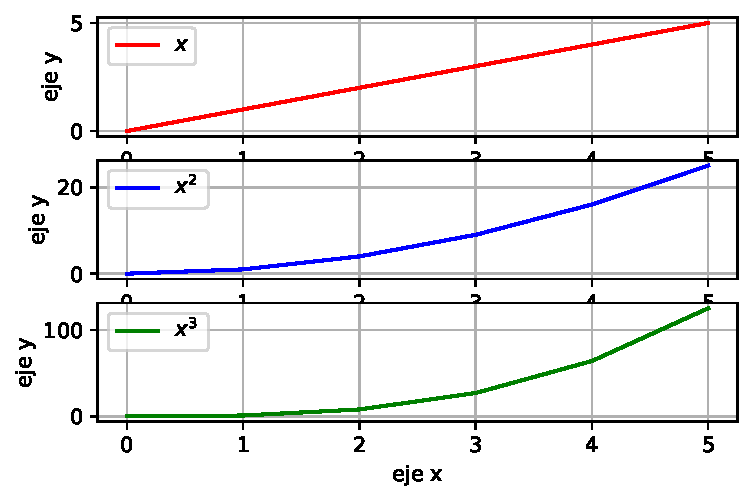
\includegraphics{unidad_6_files/figure-pdf/cell-126-output-1.pdf}

Para evitar lo anterior, definimos una función a la que le debemos
entregar los valores a graficar:

\begin{Shaded}
\begin{Highlighting}[]
\KeywordTok{def}\NormalTok{ crear\_grafico(x, y, label, ax, xlabel, ylabel, title, color):}
  \CommentTok{"""Crea un gráfico a partir de vectores con valores de los ejes x e y.}
\CommentTok{    Recibe además:}
\CommentTok{    {-} El texto para el label}
\CommentTok{    {-} El subplot a donde graficar}
\CommentTok{    {-} Un label para el eje x}
\CommentTok{    {-} Un label para el eje y}
\CommentTok{    {-} Un título para el gráfico}
\CommentTok{    {-} Un color}
\CommentTok{    El color y el eje pueden ser None. En ese caso toman valores por default"""}

  \ControlFlowTok{if}\NormalTok{ color }\OperatorTok{==} \VariableTok{None}\NormalTok{:}
\NormalTok{    color }\OperatorTok{=} \StringTok{"blue"}

  \CommentTok{\# Si sólo haremos un gráfico, no necesito indicarle la posición}
  \ControlFlowTok{if}\NormalTok{ ax }\OperatorTok{==} \VariableTok{None}\NormalTok{:}
\NormalTok{      fig, ax }\OperatorTok{=}\NormalTok{ plt.subplots()}

  \CommentTok{\# Definimos el gráfico}
\NormalTok{  ax.plot(x, y, label}\OperatorTok{=}\NormalTok{label, color}\OperatorTok{=}\NormalTok{color)}
\NormalTok{  ax.set\_xlabel(xlabel)}
\NormalTok{  ax.set\_ylabel(ylabel)}
\NormalTok{  ax.set\_title(title)}

  \ControlFlowTok{return}\NormalTok{ ax}
\end{Highlighting}
\end{Shaded}

\begin{Shaded}
\begin{Highlighting}[]
\NormalTok{fig , ax }\OperatorTok{=}\NormalTok{ plt.subplots(}\DecValTok{3}\NormalTok{)}

\CommentTok{\# En vez de copiar y pegar el código, llamo a la función crear\_grafico():}
\NormalTok{crear\_grafico(x, x\_linear, }\StringTok{"x"}\NormalTok{, ax[}\DecValTok{0}\NormalTok{], }\StringTok{"Eje x"}\NormalTok{, }\StringTok{"Eje y"}\NormalTok{, }\StringTok{"Lineal"}\NormalTok{, color}\OperatorTok{=}\StringTok{"green"}\NormalTok{)}
\NormalTok{crear\_grafico(x, x\_quadratic, }\StringTok{"$x\^{}2$"}\NormalTok{, ax[}\DecValTok{1}\NormalTok{], }\StringTok{"Eje x"}\NormalTok{, }\StringTok{"Eje y"}\NormalTok{, }\StringTok{"Cuadrática"}\NormalTok{, color}\OperatorTok{=}\StringTok{"red"}\NormalTok{)}
\NormalTok{crear\_grafico(x, x\_cubic, }\StringTok{"$x\^{}3$"}\NormalTok{, ax[}\DecValTok{2}\NormalTok{], }\StringTok{"Eje x"}\NormalTok{, }\StringTok{"Eje y"}\NormalTok{, }\StringTok{"Cúbica"}\NormalTok{, }\VariableTok{None}\NormalTok{)}

\CommentTok{\# Hacemos un for para agregar la cuadrícula y las referencias en cada axes:}
\ControlFlowTok{for}\NormalTok{ axes }\KeywordTok{in}\NormalTok{ fig.axes[:]:}
\NormalTok{  axes.grid()}
\NormalTok{  axes.legend()}
\end{Highlighting}
\end{Shaded}

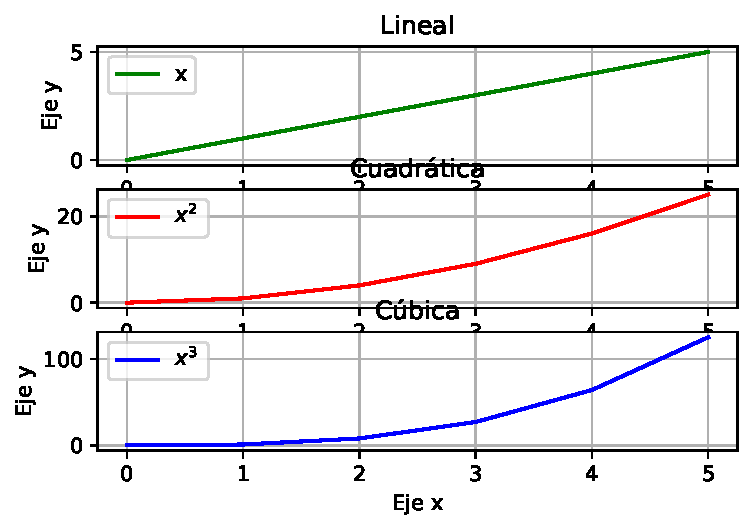
\includegraphics{unidad_6_files/figure-pdf/cell-128-output-1.pdf}

Como comentamos dentro de la función, también podemos usar
\texttt{crear\_grafico()} para un único gráfico:

\begin{Shaded}
\begin{Highlighting}[]
\NormalTok{crear\_grafico(x, x\_linear, }\StringTok{"x"}\NormalTok{, }\VariableTok{None}\NormalTok{, }\StringTok{""}\NormalTok{, }\StringTok{""}\NormalTok{, }\StringTok{""}\NormalTok{, }\StringTok{"green"}\NormalTok{)}
\end{Highlighting}
\end{Shaded}

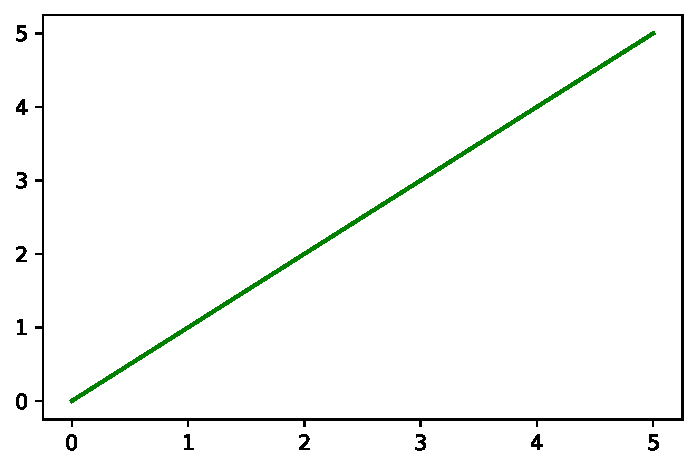
\includegraphics{unidad_6_files/figure-pdf/cell-129-output-1.pdf}

\subsection{Gráficos utilizando NumPy y
Pandas}\label{gruxe1ficos-utilizando-numpy-y-pandas}

\begin{itemize}
\tightlist
\item
  \textbf{NumPy:}
\end{itemize}

Cuando se realizó el gráfico lineal, cuadrático y cúbico de x, se
utilizaron listas de Python. A continuación puede ver lo fácil que
podría realizarse utilizando NumPy:

\begin{Shaded}
\begin{Highlighting}[]
\NormalTok{x }\OperatorTok{=}\NormalTok{ np.arange(}\DecValTok{0}\NormalTok{, }\DecValTok{6}\NormalTok{)}
\NormalTok{y\_linear }\OperatorTok{=}\NormalTok{ x}
\NormalTok{y\_quadratic }\OperatorTok{=}\NormalTok{ x}\OperatorTok{**}\DecValTok{2}
\NormalTok{y\_cubic }\OperatorTok{=}\NormalTok{ x}\OperatorTok{**}\DecValTok{3}

\NormalTok{fig, ax }\OperatorTok{=}\NormalTok{ plt.subplots(figsize}\OperatorTok{=}\NormalTok{(}\DecValTok{5}\NormalTok{, }\DecValTok{3}\NormalTok{))}

\NormalTok{ax.plot(x, y\_linear, label}\OperatorTok{=}\StringTok{\textquotesingle{}Lineal\textquotesingle{}}\NormalTok{)}
\NormalTok{ax.plot(x, y\_quadratic, label}\OperatorTok{=}\StringTok{\textquotesingle{}Cuadrático\textquotesingle{}}\NormalTok{)}
\NormalTok{ax.plot(x, y\_cubic, label}\OperatorTok{=}\StringTok{\textquotesingle{}Cúbico\textquotesingle{}}\NormalTok{)}

\NormalTok{ax.set\_title(}\StringTok{"Gráfico de múltiples curvas"}\NormalTok{)}
\NormalTok{ax.set\_xlabel(}\StringTok{\textquotesingle{}x\textquotesingle{}}\NormalTok{)}
\NormalTok{ax.set\_ylabel(}\StringTok{\textquotesingle{}y\textquotesingle{}}\NormalTok{)}
\NormalTok{ax.legend()}

\NormalTok{plt.show()}
\end{Highlighting}
\end{Shaded}

\includegraphics{unidad_6_files/figure-pdf/cell-130-output-1.pdf}

\begin{itemize}
\tightlist
\item
  \textbf{Pandas:}
\end{itemize}

Si deseamos visualizar los datos contenidos en un DataFrame, podemos
realizarlo facilmente. Definimos df:

\begin{Shaded}
\begin{Highlighting}[]
\NormalTok{data }\OperatorTok{=}\NormalTok{ \{}\StringTok{\textquotesingle{}animal\textquotesingle{}}\NormalTok{: [}\StringTok{\textquotesingle{}gato\textquotesingle{}}\NormalTok{,}\StringTok{\textquotesingle{}chinchilla\textquotesingle{}}\NormalTok{, }\StringTok{\textquotesingle{}perro\textquotesingle{}}\NormalTok{],}
        \StringTok{\textquotesingle{}edad\textquotesingle{}}\NormalTok{: [}\FloatTok{2.5}\NormalTok{, }\DecValTok{3}\NormalTok{, }\DecValTok{7}\NormalTok{],}
        \StringTok{\textquotesingle{}visitas\textquotesingle{}}\NormalTok{: [}\DecValTok{1}\NormalTok{, }\DecValTok{3}\NormalTok{, }\DecValTok{2}\NormalTok{],}
        \StringTok{\textquotesingle{}prioridad\textquotesingle{}}\NormalTok{: [}\StringTok{\textquotesingle{}si\textquotesingle{}}\NormalTok{, }\StringTok{\textquotesingle{}si\textquotesingle{}}\NormalTok{, }\StringTok{\textquotesingle{}no\textquotesingle{}}\NormalTok{]\}}

\NormalTok{df }\OperatorTok{=}\NormalTok{ pd.DataFrame(data)}
\NormalTok{df}
\end{Highlighting}
\end{Shaded}

\begin{verbatim}
/Users/aldanarastrelli/Library/Python/3.11/lib/python/site-packages/IPython/core/formatters.py:342: FutureWarning:

In future versions `DataFrame.to_latex` is expected to utilise the base implementation of `Styler.to_latex` for formatting and rendering. The arguments signature may therefore change. It is recommended instead to use `DataFrame.style.to_latex` which also contains additional functionality.
\end{verbatim}

\begin{tabular}{llrrl}
\toprule
{} &      animal &  edad &  visitas & prioridad \\
\midrule
0 &        gato &   2.5 &        1 &        si \\
1 &  chinchilla &   3.0 &        3 &        si \\
2 &       perro &   7.0 &        2 &        no \\
\bottomrule
\end{tabular}

\begin{Shaded}
\begin{Highlighting}[]
\CommentTok{\# Determino las columnas del DataFrame que queremos graficar}
\NormalTok{x\_values }\OperatorTok{=}\NormalTok{ df[}\StringTok{\textquotesingle{}animal\textquotesingle{}}\NormalTok{]}
\NormalTok{y\_values }\OperatorTok{=}\NormalTok{ df[}\StringTok{\textquotesingle{}edad\textquotesingle{}}\NormalTok{]}

\NormalTok{fig, ax }\OperatorTok{=}\NormalTok{ plt.subplots()}

\NormalTok{ax.bar(x\_values, y\_values)}

\NormalTok{ax.set\_xlabel(}\StringTok{\textquotesingle{}Animal\textquotesingle{}}\NormalTok{)}
\NormalTok{ax.set\_ylabel(}\StringTok{\textquotesingle{}Edad (años)\textquotesingle{}}\NormalTok{)}

\NormalTok{ax.set\_title(}\StringTok{"Mascotas"}\NormalTok{)}

\NormalTok{plt.show()}
\end{Highlighting}
\end{Shaded}

\includegraphics{unidad_6_files/figure-pdf/cell-132-output-1.pdf}

\bookmarksetup{startatroot}

\chapter*{Guía de Ejercicios}\label{guuxeda-de-ejercicios}
\addcontentsline{toc}{chapter}{Guía de Ejercicios}

\markboth{Guía de Ejercicios}{Guía de Ejercicios}

\section*{Recomendaciones al realizar las
guías}\label{recomendaciones-al-realizar-las-guuxedas}
\addcontentsline{toc}{section}{Recomendaciones al realizar las guías}

\markright{Recomendaciones al realizar las guías}

\begin{itemize}
\tightlist
\item
  Prestá atención al leer el enunciado. En particular:

  \begin{itemize}
  \tightlist
  \item
    Si se pide una función que \emph{devuelva} o \emph{calcule} un
    valor, la función debe tener una función \texttt{return}.
  \item
    Si se pide una función que \emph{imprima} un valor, la función debe
    tener un \texttt{print}.
  \item
    Si se pide una función que \emph{pida} o \emph{pregunte} algo al
    usuario, la función debe tener un \texttt{input}.
  \item
    A menos que se diga específicamente ``pedirle al usuario'', no es
    necesario que el programa contenga \texttt{input}. En todo caso,
    hacer que la función reciba el o los datos por parámetro.
  \end{itemize}
\item
  Cada ejercicio puede tener muchas soluciones posibles. Una vez que
  encuentres una solución, en lugar de pasar al siguiente ejercicio,
  pensá si se te ocurre una solución cuya codificación sea más simple.
\item
  Es muy importante que el código sea lo más claro y legible posible.

  \begin{itemize}
  \tightlist
  \item
    En particular, nombres de funciones y variables deben ser
    descriptivos.
  \item
    También prestá atención a los espacios en blanco y a la indentación.
  \end{itemize}
\item
  No documentes en exceso, pero tampoco ahorres documentación necesaria.
\item
  Probá siempre que el código cumpla con lo solicitado.
\end{itemize}

\begin{tcolorbox}[enhanced jigsaw, bottomrule=.15mm, leftrule=.75mm, opacityback=0, colback=white, toprule=.15mm, bottomtitle=1mm, opacitybacktitle=0.6, rightrule=.15mm, left=2mm, arc=.35mm, coltitle=black, title=\textcolor{quarto-callout-note-color}{\faInfo}\hspace{0.5em}{Discord}, breakable, toptitle=1mm, colframe=quarto-callout-note-color-frame, titlerule=0mm, colbacktitle=quarto-callout-note-color!10!white]

La materia usa Discord como plataforma adicional para la resolución de
los ejercicios de las guias.\\
Tengan a bien leer con atención el mensaje de bienvenida y las reglas de
convivencia. Pueden ingresar al servidor a través del siguiente link.

\end{tcolorbox}

\section*{Guía 1: Introducción a la Algoritmia y la
Programación}\label{guuxeda-1-introducciuxf3n-a-la-algoritmia-y-la-programaciuxf3n}
\addcontentsline{toc}{section}{Guía 1: Introducción a la Algoritmia y la
Programación}

\markright{Guía 1: Introducción a la Algoritmia y la Programación}

\begin{tcolorbox}[enhanced jigsaw, bottomrule=.15mm, leftrule=.75mm, opacityback=0, colback=white, toprule=.15mm, bottomtitle=1mm, opacitybacktitle=0.6, rightrule=.15mm, left=2mm, arc=.35mm, coltitle=black, title=\textcolor{quarto-callout-note-color}{\faInfo}\hspace{0.5em}{Recomendación}, breakable, toptitle=1mm, colframe=quarto-callout-note-color-frame, titlerule=0mm, colbacktitle=quarto-callout-note-color!10!white]

En esta guía nos dedicaremos a introducirnos en los conceptos de
programación y algoritmo. Para los primeros seis ejercicios, te
recomendamos ver \href{https://www.youtube.com/watch?v=cDA3_5982h8}{este
video} para recordar cómo entiende la computadora nuestras
instrucciones.

\end{tcolorbox}

\begin{enumerate}
\def\labelenumi{\arabic{enumi}.}
\item
  Se tiene que explicar a una máquina exactamente cómo servir un vaso de
  jugo (de los que vienen en cartón) de la heladera. Recordando la
  definición de algoritmo, hacer una descripción paso a paso de lo que
  se tiene que hacer y usar para lograr el objetivo. Pista: No vas a
  necesitar nada de código en este ejercicio, sólo nombrar los pasos.
\item
  Se tiene que explicar a una máquina exactamente cómo hacer una tostada
  con queso, pensá qué ingredientes se necesitan con sus cantidades,
  cómo tiene que ser el espacio de trabajo y los elementos que va a
  necesitar usar. Recordando la definición de algoritmo, hacer una
  descripción paso a paso de lo que se tiene que hacer y usar para hacer
  una tostada con queso. Pista: No vas a necesitar nada de código en
  este ejercicio, sólo nombrar los pasos.
\item
  Se te pide que organices una colecta de alimentos no perecederos por
  la Ciudad de Buenos Aires. Contamos con algunos automóviles y
  camionetas de voluntarios, un listado de donaciones, listado de los
  alimentos a donar, la disponibilidad horaria y la dirección en la cual
  se dejan los alimentos. La colecta se realiza en un solo día. ¿Cómo la
  organizarías? Pista: No vas a necesitar nada de código en este
  ejercicio, sólo nombrar los pasos.
\item
  Tenés que enviar invitaciones personalizadas para tu cumpleaños. Cada
  invitación tiene que mencionar el nombre de la persona y la relación
  que tiene con vos. Contamos con una impresora a la que le das el texto
  a enviar, un listado con los nombres de los invitados y la relación
  que cada uno tiene con vos. ¿Cómo redactarías el texto de la
  invitación? Pista: No vas a necesitar nada de código en este
  ejercicio, sólo nombrar los pasos.
\item
  Se te encargó definir qué datos son necesarios para el registro de
  estudiantes en un curso de inglés. ¿Qué datos crees que deberían ser
  obligatorios y cuáles opcionales? ¿Y si el curso es de cocina? Pista:
  No vas a necesitar nada de código en este ejercicio, sólo nombrar los
  pasos.
\item
  Contás con un listado de cosas a comprar y tenes que ir a un
  supermercado que cuenta con distintas góndolas o pasillos. Cada
  góndola o pasillo puede contar con varios, uno o ninguno de los
  productos de tu lista. ¿Cuál sería el listado de instrucciones para
  poder terminar lo más rápido posible? Pista: No vas a necesitar nada
  de código en este ejercicio, sólo nombrar los pasos.
\item
  Con el anexo de Replit de la Unidad 1, realizá tu primer programa:
  hacé que se imprima por pantalla un \texttt{“¡Hola\ mundo!”}.
\end{enumerate}

\section*{Guía 2: Tipos de Datos, Expresiones y
Funciones}\label{guuxeda-2-tipos-de-datos-expresiones-y-funciones}
\addcontentsline{toc}{section}{Guía 2: Tipos de Datos, Expresiones y
Funciones}

\markright{Guía 2: Tipos de Datos, Expresiones y Funciones}

\begin{enumerate}
\def\labelenumi{\arabic{enumi}.}
\item
  Guardar el texto ``Hola, Mundo!'' en una variable e imprimirla por
  pantalla.
\item
  Guardar los números 1, 2 y 3 en tres variables distintas e imprimirlos
  por pantalla.
\item
  \begin{enumerate}
  \def\labelenumii{\alph{enumii}.}
  \tightlist
  \item
    Guardar los números 1, 2 y 3 en tres variables distintas y luego
    sumarlos e imprimir el resultado por pantalla.\\
  \item
    Repetir con las distintas operaciones disponibles que se vieron en
    la unidad 2: resta, multiplicación, división, división entera,
    resto, potencia; combinando los números entre sí.
  \end{enumerate}
\item
  Crear un programa que le solicite al usuario:

  \begin{enumerate}
  \def\labelenumii{\alph{enumii}.}
  \tightlist
  \item
    Su nombre y lo imprima por pantalla.
  \item
    Su edad y la imprima por pantalla.
  \item
    Su edad, le sume 1, y la imprima por pantalla.
  \end{enumerate}
\item
  Crear un programa que le solicite al usuario un número, y que devuelva
  el resto obtenido de dividirlo por 2.\\
  ¿Qué operador vimos para obtener el resto?
\item
  Escribir un programa que le pida al usuario su año de nacimiento, y
  que le diga qué edad tiene en el año actual.
\item
  Crear un programa que le solicite al usuario 5 enteros y que muestre
  por pantalla el promedio de ellos. Hacerlo de dos formas:

  \begin{enumerate}
  \def\labelenumii{\alph{enumii}.}
  \tightlist
  \item
    Primero, usando 5 variables para cada entero.
  \item
    Después, usando una sola variable para almacenar la suma de los 5
    enteros. ¿Cómo se te ocurre que podrías hacer?
  \end{enumerate}
\item
  Crear una \textbf{función} que reciba un número y que devuelva el
  valor absoluto.
\item
  Crear una \textbf{función} que reciba un número y que devuelva
  \texttt{True} si es par, y \texttt{False} si es impar.
\item
  Crear una \textbf{función} que reciba un número y un string, y que
  devuelva ambos concatenados dentro de un nuevo string.
\item
  Crear una \textbf{función} que reciba dos enteros y que devuelva el
  resto y el cociente entre ellos.
\item
  Crear una función que le pida al usuario su nombre y apellido, e los
  imprima con el siguiente formato: ``Apellido, Nombre''.
\item
  Hacer una \textbf{función} que reciba una palabra y devuelva la
  cantidad de letras que tiene.
\item
  \begin{enumerate}
  \def\labelenumii{\alph{enumii}.}
  \tightlist
  \item
    Hacer una \textbf{función} que reciba una palabra y que imprima los
    primeros 5 caracteres únicamente. Ejemplo: Si se recibe
    ``pensamiento'' se debe imprimir ``pensa''.
  \item
    Hacer una \textbf{función} que reciba una palabra y que imprima sólo
    los caracteres ubicados en posiciones pares. Ejemplo: Si se recibe
    ``pensamiento'' se debe imprimir ``pnaino''.
  \item
    Hacer una \textbf{función} que reciba una palabra y que imprima la
    palabra dada vuelta. Ejemplo: Si se recibe ``materia'' se debe
    imprimir ``airetam''.
  \end{enumerate}
\item
  Hacer una \textbf{funcion} que reciba una palabra, le borre todas las
  letras ``a'' e imprima el resultado por pantalla. Pista: usar una
  función predefinida de Python. Ejemplo: Si se recibe ``casa'' se debe
  imprimir ``cs''.
\item
  Analizar qué tipo de dato (o error) se obtiene al hacer las siguientes
  operaciones:

  \begin{enumerate}
  \def\labelenumii{\alph{enumii}.}
  \tightlist
  \item
    \texttt{5\ /\ 2}
  \item
    \texttt{5\ //\ 2}
  \item
    \texttt{5\ \%\ 2}
  \item
    \texttt{5\ **\ 2}
  \item
    \texttt{5.0\ /\ 2}
  \item
    \texttt{5.0\ //\ 2}
  \item
    \texttt{5.0\ \%\ 2}
  \item
    \texttt{5.0\ **\ 2}
  \item
    \texttt{5\ /\ 2.0}
  \item
    \texttt{5\ //\ 2.0}
  \item
    \texttt{5\ \%\ 2.0}
  \item
    \texttt{5\ **\ 2.0}
  \item
    \texttt{5.0\ /\ 2.0}
  \item
    \texttt{5.0\ //\ 2.0}
  \item
    \texttt{5.0\ \%\ 2.0}
  \item
    \texttt{5.0\ **\ 2.0}
  \item
    \texttt{"Hola"\ *\ 2}
  \item
    \texttt{"Hola"\ +\ 2}
  \item
    \texttt{"Hola"\ +\ "2"}
  \item
    \texttt{x\ =\ "Hola"}\strut \\
    \texttt{x\ +=\ "\ mundo"}
  \end{enumerate}
\item
  \begin{enumerate}
  \def\labelenumii{\alph{enumii}.}
  \tightlist
  \item
    Escribir una función que convierta un valor dado en grado Celsius, a
    Fahrenheit. Recordar que la fórmula para la conversión es:
    \texttt{F\ =\ 9/5\ *\ C\ +\ 32}.
  \item
    Escribir una función que convierta un valor dado en grados
    Fahrenheit, a Celsius. Usar la misma fórmula anterior.
  \end{enumerate}
\item
  Escribir una función que calcule el área de un triángulo recibiendo
  como parámetros su base y su altura.
\item
  Siendo el cálculo de la norma de un vector \(v\) en \(R^3\):\\
  \[||v|| = \sqrt{v_1^2 + v_2^2 + v_3^2}\]\\
  Escribir una función que calcule la norma de un vector en R3
  recibiendo como parámetros las 3 componentes \(v_1\), \(v_2\) y
  \(v_3\) del mismo.
\item
  \textbf{Desafío} (no obligatorio): Calcular el área de un rectángulo
  (alineado con los ejes \(x\) e \(y\)), dadas sus coordenadas \(x_1\),
  \(x_2\), \(y_1\) e \(y_2\).
\end{enumerate}

\section*{Guía 3: Estructuras de
Control}\label{guuxeda-3-estructuras-de-control}
\addcontentsline{toc}{section}{Guía 3: Estructuras de Control}

\markright{Guía 3: Estructuras de Control}

\subsection*{1. Decisiones}\label{decisiones-1}
\addcontentsline{toc}{subsection}{1. Decisiones}

\begin{enumerate}
\def\labelenumi{\arabic{enumi}.}
\item
  Escribir una función que, dado un número entero \(n\), calcule si es
  impar o no.
\item
  Escribir una implementación propia de la función \(abs\), que devuelva
  el valor absoluto de cualquier valor que reciba. Ejemplo:
  \texttt{mi\_abs(5)} devuelve \texttt{5} y \texttt{mi\_abs(-5)}
  devuelve \texttt{5}. Pista: No se puede usar la función predefinida
  \texttt{abs}.
\item
  Escribir una función que reciba un número y devuelva \texttt{True} si
  es entero y \texttt{False} si no lo es. Pista: no se puede usar la
  función \texttt{isinstance}.
\item
  Escribir una función para determinar si una letra recibida es vocal o
  no. La misma debe devolver un valor booleano. Luego, escribir una
  función para determinar si una letra es consonante o no.

  \begin{enumerate}
  \def\labelenumii{\alph{enumii}.}
  \tightlist
  \item
    Resolver \emph{sin} el uso de \texttt{in} ni \texttt{not\ in}.
  \item
    Resolver \emph{usando} \texttt{in} y \texttt{not\ in}.
  \item
    Resolver para que la función identifique tanto mayúsculas como
    minúsculas. Pista: investigar los métodos \texttt{lower} y
    \texttt{upper} de string.
  \end{enumerate}
\end{enumerate}

\begin{tcolorbox}[enhanced jigsaw, bottomrule=.15mm, leftrule=.75mm, opacityback=0, colback=white, toprule=.15mm, bottomtitle=1mm, opacitybacktitle=0.6, rightrule=.15mm, left=2mm, arc=.35mm, coltitle=black, title=\textcolor{quarto-callout-tip-color}{\faLightbulb}\hspace{0.5em}{Tip: \texttt{in} y \texttt{not\ in}}, breakable, toptitle=1mm, colframe=quarto-callout-tip-color-frame, titlerule=0mm, colbacktitle=quarto-callout-tip-color!10!white]

¿Conocés el uso de \texttt{in}?

Para saber si un elemento está en una lista o en un string, podemos usar
\texttt{in} y \texttt{not\ in}. Por ejemplo:

\begin{Shaded}
\begin{Highlighting}[]
\CommentTok{\textquotesingle{}a\textquotesingle{}} \KeywordTok{in} \StringTok{\textquotesingle{}hola\textquotesingle{}}
\end{Highlighting}
\end{Shaded}

\begin{verbatim}
True
\end{verbatim}

\begin{Shaded}
\begin{Highlighting}[]
\CommentTok{\textquotesingle{}w\textquotesingle{}} \KeywordTok{in} \StringTok{\textquotesingle{}hola\textquotesingle{}}
\end{Highlighting}
\end{Shaded}

\begin{verbatim}
False
\end{verbatim}

\begin{Shaded}
\begin{Highlighting}[]
\CommentTok{\textquotesingle{}w\textquotesingle{}} \KeywordTok{not} \KeywordTok{in} \StringTok{\textquotesingle{}hola\textquotesingle{}}
\end{Highlighting}
\end{Shaded}

\begin{verbatim}
True
\end{verbatim}

\begin{Shaded}
\begin{Highlighting}[]
\CommentTok{\textquotesingle{}casa\textquotesingle{}} \KeywordTok{in}\NormalTok{ [}\StringTok{\textquotesingle{}cama\textquotesingle{}}\NormalTok{, }\StringTok{\textquotesingle{}mesa\textquotesingle{}}\NormalTok{, }\StringTok{\textquotesingle{}silla\textquotesingle{}}\NormalTok{]}
\end{Highlighting}
\end{Shaded}

\begin{verbatim}
False
\end{verbatim}

\end{tcolorbox}

\begin{enumerate}
\def\labelenumi{\arabic{enumi}.}
\setcounter{enumi}{4}
\item
  Escribir funciones que resuelvan los siguientes problemas:

  \begin{enumerate}
  \def\labelenumii{\alph{enumii}.}
  \tightlist
  \item
    Dado un año, que devuelva si es bisiesto. Nota: un año es bisiesto
    si es un número divisible por 4, pero no si es divisible por 100,
    excepto que también sea divisible por 400.
  \item
    Dado un mes y un año, que devuelva la cantidad de días
    correspondientes.
  \item
    Pedirle al usuario su día y mes de cumpleaños. El programa debe
    imprimir un mensaje indicando a qué signo corresponde el usuario.
  \end{enumerate}

\begin{verbatim}
Aries: 21 de marzo al 20 de abril.
Tauro: 21 de abril al 20 de mayo.
Geminis: 21 de mayo al 21 de junio.
Cancer: 22 de junio al 23 de julio.
Leo: 24 de julio al 23 de agosto.
Virgo: 24 de agosto al 23 de septiembre.
Libra: 24 de septiembre al 22 de octubre.
Escorpio: 23 de octubre al 22 de noviembre.
Sagitario: 23 de noviembre al 21 de diciembre.
Capricornio: 22 de diciembre al 20 de enero.
Acuario: 21 de enero al 19 de febrero.
Piscis: 20 de febrero al 20 de marzo.
\end{verbatim}
\item
  Piedra, papel o tijera: escribir un programa de ``Piedra, papel o
  tijera'' tal que sea imposible que el usuario gane. El usuario debe
  ingresar \textbf{R} (piedra), \textbf{P} (papel), o \textbf{T}
  (tijera) y la computadora debe siempre ganarle. Ejemplo:

\begin{verbatim}
¡Piedra (R), papel (P) o tijera (T)!
Ingrese jugada: R
¡Papel! ¡Gané!
\end{verbatim}

\begin{verbatim}
¡Piedra (R), papel (P) o tijera (T)!
Ingrese jugada: P
¡Tijera! ¡Gané!
\end{verbatim}

\begin{verbatim}
¡Piedra (R), papel (P) o tijera (T)!
Ingrese jugada: T
¡Piedra! ¡Gané!
\end{verbatim}

\begin{verbatim}
¡Piedra (R), papel (P) o tijera (T)!
Ingrese jugada: M
Esa jugada no está disponible.
\end{verbatim}
\item
  Suponiendo que el primer día del año fue lunes, escribir una función
  que reciba un número con el día del año (de 1 a 366) y devuelva el día
  de la semana que le toca. Por ejemplo: si se recibe `3', debe devolver
  ``miércoles'', y si se recibe `9', debe devolver ``martes''.
\end{enumerate}

\subsection*{2. Ciclos}\label{ciclos-1}
\addcontentsline{toc}{subsection}{2. Ciclos}

\begin{enumerate}
\def\labelenumi{\arabic{enumi}.}
\item
  Escribir función que:

  \begin{enumerate}
  \def\labelenumii{\alph{enumii}.}
  \tightlist
  \item
    Imprima por pantalla todos los números entre 10 y 20.
  \item
    Salude a todas las personas de esta lista
    \texttt{{[}Flaminia,\ Serena,\ Agustina,\ Priscila,\ Sol,\ Agostina,\ Iara,\ Lu{]}}
    con el mensaje
    \texttt{"Hola\ \textless{}nombre\textgreater{}!\ Vamos\ a\ aprender\ a\ programar"}.
  \item
    Le pida al usuario que ingrese 5 números y le muestre la suma total
    de todos ellos.
  \item
    Imprima por pantalla todos los números entre 100 y 199 que sean
    divisibles por 7.
  \item
    Reciba dos números, y recorra todos los números entre ellos,
    imprimiendo en pantalla si es par o impar. Por ejemplo, recibiendo 1
    y 3, debe imprimir:
  \end{enumerate}

\begin{verbatim}
1 es impar
2 es par
3 es impar
\end{verbatim}
\item
  Se quiere hacer un programa para enseñar a los niños las tablas de
  multiplicar del 1 al 10. Crear una función que reciba un número e
  imprima por pantalla la tabla de multiplicar de ese número. Ejemplo:

\begin{verbatim}
mostrar_tablas_para(1)
\end{verbatim}

  debe imprimir:

\begin{verbatim}
1 x 1 = 1
1 x 2 = 2
1 x 3 = 3
1 x 4 = 4
1 x 5 = 5
1 x 6 = 6
1 x 7 = 7
1 x 8 = 8
1 x 9 = 9
1 x 10 = 10
\end{verbatim}

\begin{verbatim}
mostrar_tablas_para(-2)
\end{verbatim}

  debe imprimir:

\begin{verbatim}
Error: El número debe ser positivo y estar entre 1 y 10
\end{verbatim}
\item
  Crear una función que cante el feliz cumpleaños. Dado un entero, debe
  imprimir `Que los cumplas feliz' en distintas líneas por esa cantidad
  de veces.
\item
  \begin{enumerate}
  \def\labelenumii{\alph{enumii}.}
  \tightlist
  \item
    Necesitamos escribir un programa de cobro en el supermercado. La
    función debe recibir un número entero que representa el monto a
    pagar y debe permitir al usuario que ingrese valores, hasta que el
    pago se haya realizado en su totalidad. Además, le debe ir indicando
    cuánto le queda por pagar. El programa no da vuelto.
  \end{enumerate}

  Ejemplo:

\begin{verbatim}
Su total a pagar es: 500
Ingrese el monto a pagar: 100
Pendientes: 400. Ingrese el monto a pagar: 200
Pendientes: 200. Ingrese el monto a pagar: 200
Pendientes: 0. Gracias por su compra.
\end{verbatim}

  \begin{enumerate}
  \def\labelenumii{\alph{enumii}.}
  \setcounter{enumii}{1}
  \tightlist
  \item
    Hacer que el programa anterior dé vuelto:
  \end{enumerate}

  Ejemplo:

\begin{verbatim}
Su total a pagar es: 500
Ingrese el monto a pagar: 100
Pendientes: 400. Ingrese el monto a pagar: 200
Pendientes: 200. Ingrese el monto a pagar: 300
Pendientes: 0. Su vuelto es: 100. Gracias por su compra.
\end{verbatim}
\item
  Escribir un programa que le pida al usuario que ingrese un número.
  Para ese número, se imprime la tabla de multiplicar del 1 al 10.
  Luego, se le vuelve a pedir otro número. Si el usuario ingresa ``X'',
  el programa debe terminar. El usuario debe poder ingresar números
  indefinidamente hasta que ingrese ``X''. Se puede reutilizar la
  función del ejercicio 9 de esta guía.

  Ejemplo:

\begin{verbatim}
Hola! Esto es Tablas de Multiplicar
Ingrese un número o "X" para salir: 1
1 x 1 = 1
1 x 2 = 2
1 x 3 = 3
1 x 4 = 4
1 x 5 = 5
1 x 6 = 6
1 x 7 = 7
1 x 8 = 8
1 x 9 = 9
1 x 10 = 10
Ingrese un número o "X" para salir: -2
Error: El número debe ser positivo y estar entre 1 y 10
Ingrese un número o "X" para salir: X
¡Adios!
\end{verbatim}
\item
  \textbf{Manejo de contraseñas}

  \begin{enumerate}
  \def\labelenumii{\alph{enumii}.}
  \tightlist
  \item
    Escribir un programa que contenga una contraseña inventada, que le
    pregunte al usuario la contraseña, y no le permita continuar hasta
    que la haya ingresado correctamente.
  \item
    Modificar el programa anterior para que solamente permita una
    cantidad fija de intentos.
  \item
    Modificar el programa anterior para que sea una función que devuelva
    si el usuario ingresó o no la contraseña correctamente, mediante un
    valor booleano (\texttt{True} o \texttt{False}).
  \end{enumerate}
\item
  \begin{enumerate}
  \def\labelenumii{\alph{enumii}.}
  \item
    Hacer una función que reciba un número del 1 al 10, y luego permita
    al usuario poder adivinar ese número, ingresando valores
    repetidamente. Para cada ingreso del usuario, el programa debe
    indicarle si su numero es menor o mayor al número a adivinar. Una
    vez que el usuario ingresa el número correcto, lo felicita y
    termina.
  \item
    Repetir permitiendo únicamente 3 intentos.
  \item
    Repetir generando el número aleatoriamente de la siguiente forma
    dentro de la función, sin recibirlo por parámetro:
  \end{enumerate}
\end{enumerate}

\begin{Shaded}
\begin{Highlighting}[]
\ImportTok{import}\NormalTok{ random}
\NormalTok{numero\_a\_adivinar }\OperatorTok{=}\NormalTok{ random.randint(}\DecValTok{1}\NormalTok{, }\DecValTok{10}\NormalTok{)}
\BuiltInTok{print}\NormalTok{(numero\_a\_adivinar)}
\end{Highlighting}
\end{Shaded}

\begin{verbatim}
3
\end{verbatim}

\begin{tcolorbox}[enhanced jigsaw, bottomrule=.15mm, leftrule=.75mm, opacityback=0, colback=white, toprule=.15mm, bottomtitle=1mm, opacitybacktitle=0.6, rightrule=.15mm, left=2mm, arc=.35mm, coltitle=black, title=\textcolor{quarto-callout-note-color}{\faInfo}\hspace{0.5em}{Tip: Bibliotecas}, breakable, toptitle=1mm, colframe=quarto-callout-note-color-frame, titlerule=0mm, colbacktitle=quarto-callout-note-color!10!white]

¿Sabías que Python tiene muchas bibliotecas que podés usar para hacer
cosas más complejas? Por ejemplo, la biblioteca \texttt{random} tiene
funciones para generar números aleatorios. También hay otras bibliotecas
como \texttt{Pandas} para trabajar con datos, \texttt{Matplotlib} para
hacer gráficos, \texttt{Numpy} para trabajar con matrices, y muchas más.
Vamos a estar viendo estas tres en la última unidad de la materia.

Una biblioteca es un conjunto de funciones que alguien más escribió y
que podemos usar en nuestros programas. Para usar una biblioteca,
primero tenemos que importarla. Por ejemplo, para usar la biblioteca
\texttt{random}, tenemos que poner \texttt{import\ random} al principio
de nuestro programa (arriba de todo en nuestro archivo). Luego, podemos
usar las funciones de la biblioteca, como
\texttt{random.randint(1,\ 10)}.

\end{tcolorbox}

\begin{enumerate}
\def\labelenumi{\arabic{enumi}.}
\setcounter{enumi}{7}
\item
  \begin{enumerate}
  \def\labelenumii{\alph{enumii}.}
  \tightlist
  \item
    Queremos modelar una máquina de sacar juguetes. Debemos hacer una
    función que reciba un número que representa la cantidad de fichas
    \(x\) que necesita la máquina para funcionar. Se debe imprimir un
    mensaje en pantalla que indique ``Ingresá \(x\) fichas para
    comenzar''. El usuario deberá ingresar entonces letras ``F'', que
    representan a las fichas. Notar que si se ingresa algo distinto a
    ``F'', se ignora.
  \end{enumerate}

  Se debe seguir solicitando fichas siempre que no se haya alcanzado la
  cantidad necesaria para funcionar. Cuando se haya alcanzado la
  cantidad necesaria, se debe imprimir un mensaje que indique ``¡A
  jugar!''. Ejemplo:

\begin{verbatim}
Ingresá 2 fichas para comenzar: F
Ingresá 2 fichas para comenzar: B
Ingresá 2 fichas para comenzar: Hola
Ingresá 2 fichas para comenzar: F
¡A jugar!
\end{verbatim}

  \begin{enumerate}
  \def\labelenumii{\alph{enumii}.}
  \setcounter{enumii}{1}
  \tightlist
  \item
    Modificar el programa anterior para que vaya mostrando la cantidad
    de fichas que faltan para comenzar a jugar. Ejemplo:
  \end{enumerate}

\begin{verbatim}
Ingresá 2 fichas para comenzar: F
Ingresá 1 fichas para comenzar: B
Ingresá 1 fichas para comenzar: ficha
Ingresá 1 fichas para comenzar: F
¡A jugar!
\end{verbatim}
\item
  Crear una función que calcule si un número es primo o no. Un número es
  primo cuando solamente es divisible por sí mismo y por 1. Pista: usar
  el operador módulo \texttt{\%}.
\item
  \textbf{Desafío} (obligatorio): Crear una función que reciba un número
  entero e imprima los números primos entre 0 y el número ingresado.
\item
  \textbf{Desafío} (obligatorio):

  \begin{enumerate}
  \def\labelenumii{\alph{enumii}.}
  \item
    Crear una función que reciba dos números, y devuelva la suma de
    todos los números múltiplos de 7 entre esos dos números. Por
    ejemplo, si recibe 3 y 25, debe devolver 7 + 14 + 21 = 42. Si recibe
    3 y 4, debe devolver 0, ya que no hay múltiplos de 7 entre esos dos
    números.
  \item
    Repetir calculando el promedio en vez de la suma.
  \item
    Repetir calculando únicamente el promedio entre los primeros 3
    múltiplos de 7 encontrados. Pista: usar \texttt{break}.
  \item
    Repetir calculando únicamente el promedio entre los múltiplos de 7
    encontrados que no sean múltiplos de 2. Pista: usar
    \texttt{continue}.
  \end{enumerate}
\item
  \textbf{Desafío} (obligatorio):

  \begin{enumerate}
  \def\labelenumii{\alph{enumii}.}
  \tightlist
  \item
    Escribir una función que dada la cantidad de ejercicios de un
    examen, y el porcentaje de ejercicios bien resueltos necesario para
    aprobar dicho examen, revise un grupo de exámenes.
  \end{enumerate}

  Para ello, en cada paso debe preguntarle al usuario la cantidad de
  ejercicios resueltos por el alumno, o pedirle que ingrese ``*'' para
  salir. Debe mostrar por pantalla el porcentaje correspondiente a la
  cantidad de ejercicios resueltos respecto a la cantidad de ejercicios
  del examen y una leyenda que indique si aprobó o no.

  \begin{enumerate}
  \def\labelenumii{\alph{enumii}.}
  \setcounter{enumii}{1}
  \tightlist
  \item
    Adicional al punto anterior: imprimir un mensaje informándole al
    usuario la cantidad de ejercicios y el \% de aprobación.\\
    Validar que el usuario siempre ingrese números positivos y menor o
    iguales a la cantidad de ejercicios del examen, o ``*``. De lo
    contrario, mostrar un mensaje de error y volver a pedirle el dato al
    usuario.
  \end{enumerate}
\end{enumerate}

\section*{Guía 4: Tipos de Estructuras de
Datos}\label{guuxeda-4-tipos-de-estructuras-de-datos}
\addcontentsline{toc}{section}{Guía 4: Tipos de Estructuras de Datos}

\markright{Guía 4: Tipos de Estructuras de Datos}

\subsection*{1. Cadenas de caracteres}\label{cadenas-de-caracteres-1}
\addcontentsline{toc}{subsection}{1. Cadenas de caracteres}

\begin{enumerate}
\def\labelenumi{\arabic{enumi}.}
\item
  Escribir funciones que dada una cadena y un caracter:

  \begin{enumerate}
  \def\labelenumii{\alph{enumii}.}
  \item
    Inserte el caracter entre cada letra de la cadena. Ejemplo:
    \texttt{\textquotesingle{}separar\textquotesingle{}} y
    \texttt{\textquotesingle{}-\textquotesingle{}} debería devolver
    \texttt{\textquotesingle{}s-e-p-a-r-a-r\textquotesingle{}}.\\
  \item
    Reemplace todos los espacios por el caracter. Ejemplo:
    \texttt{\textquotesingle{}mi\ archivo\ de\ texto.txt\textquotesingle{}}
    y \texttt{\textquotesingle{}\_}' debería devolver
    \texttt{\textquotesingle{}mi\_archivo\_de\_texto.txt\textquotesingle{}}.\\
  \item
    Reemplace todos los dígitos de la cadena por el caracter. Ejemplo:
    \texttt{\textquotesingle{}su\ clave\ es:\ 1540\textquotesingle{}} y
    \texttt{\textquotesingle{}*\textquotesingle{}} debería devolver
    \texttt{\textquotesingle{}su\ clave\ es:\ ****\textquotesingle{}}.\\
  \item
    Inserte el caracter cada 3 dígitos en la cadena. Ejemplo:
    \texttt{\textquotesingle{}2552552550\textquotesingle{}} y
    \texttt{\textquotesingle{}.\textquotesingle{}} debería devolver
    \texttt{\textquotesingle{}255.255.255.0\textquotesingle{}}
  \item
    Modificar todas las anteriores para que, adicionalmente, reciba un
    parámetro que indique la cantidad máxima de reemplazos o inserciones
    a realizar. Ejemplo:
    \texttt{\textquotesingle{}su\ clave\ es:\ 1540\textquotesingle{}},
    \texttt{\textquotesingle{}*\textquotesingle{}} y \texttt{3} debería
    devolver
    \texttt{\textquotesingle{}su\ clave\ es:\ ***0\textquotesingle{}}.
  \end{enumerate}
\item
  Escribir una función que reciba una cadena que contiene un largo
  número entero y devuelva una cadena con el número y las separaciones
  de miles. Por ejemplo, si recibe \texttt{1234567890}, debe devolver
  \texttt{1.234.567.890}. Cuidado: no es lo mismo \texttt{123.456.789.0}
  que \texttt{1.234.567.890}. Tienen que ser separaciones de miles y
  quedar un número válido.
\item
  Escribir funciones que dada una cadena de caracteres:

  \begin{enumerate}
  \def\labelenumii{\alph{enumii}.}
  \tightlist
  \item
    Devuelva la primera letra de cada palabra. Ejemplo: si se recibe
    \texttt{Ciclo\ Básico\ Común} se debe devolver \texttt{CBC}.
  \item
    Indique si se trata de un palíndromo. Por ejemplo,
    \texttt{anita\ lava\ la\ tina} es un palíndromo (se lee igual de
    izquierda a derecha que de derecha a izquierda).
  \end{enumerate}
\item
  Escribir funciones que dadas dos cadenas de caracteres:

  \begin{enumerate}
  \def\labelenumii{\alph{enumii}.}
  \tightlist
  \item
    Indique si la segunda cadena es subcadena de la primera. Por
    ejemplo, \texttt{\textquotesingle{}compu\textquotesingle{}} es
    subcadena de
    \texttt{\textquotesingle{}computacional\textquotesingle{}}.
  \item
    Devuelva la que sea anterior en orden alfábetico. Por ejemplo, si
    recibe \texttt{\textquotesingle{}kde\textquotesingle{}} y
    \texttt{\textquotesingle{}gnome\textquotesingle{}} debe devolver
    \texttt{\textquotesingle{}gnome\textquotesingle{}}.
  \end{enumerate}
\item
  Escribir una función que, dada una cadena de caracteres, devuelva una
  lista con cada uno de los caracteres que la componen en mayúscula.
  Ejemplo: \texttt{\textquotesingle{}Hola\textquotesingle{}} debe
  devolver
  \texttt{{[}\textquotesingle{}H\textquotesingle{},\ \textquotesingle{}O\textquotesingle{},\ \textquotesingle{}L\textquotesingle{},\ \textquotesingle{}A\textquotesingle{}{]}}.
  Restricción: no se permite el uso de ciclos for/while. Pista: Buscá en
  el apunte cómo usar \texttt{map}.
\item
  Escribir una función que, dada una cadena de caracteres, devuelva una
  tupla con cada uno de los caracteres que no es una vocal. Ejemplo:
  \texttt{\textquotesingle{}Algoritmos\textquotesingle{}} debe devolver
  \texttt{(\textquotesingle{}l\textquotesingle{},\ \textquotesingle{}g\textquotesingle{},\ \textquotesingle{}r\textquotesingle{},\ \textquotesingle{}t\textquotesingle{},\ \textquotesingle{}m\textquotesingle{},\ \textquotesingle{}s\textquotesingle{})}.
  Restricción: no se permite el uso de ciclos for/while.
\item
  Escribir una función que, dada una cadena de caracteres, devuelva el
  número de índice de posición del último caracter. Por ejemplo, para la
  cadena \texttt{\textquotesingle{}Hola\textquotesingle{}} debe devolver
  \texttt{3}. Restricción: no se permite el uso de ciclos for/while.
\item
  \textbf{Desafío} (obligatorio):

  \begin{enumerate}
  \def\labelenumii{\alph{enumii}.}
  \item
    Se quiere implementar un buscador dentro de un editor de texto, que
    permita encontrar todas las ocurrencias de una palabra en un texto.
    Para ello, se debe implementar una función que reciba como parámetro
    una palabra y un texto, y que devuelva la primer aparición de la
    palabra en el texto. Pista: \texttt{index} arrojará un error si la
    subcadena no se encuentra. ¿Qué otro método tenemos disponible para
    buscar subcadenas?
  \item
    Modificar la función anterior para que devuelva una lista con las
    posiciones de inicio de cada ocurrencia de la palabra dentro del
    texto. Ejemplo: si se busca
    \texttt{\textquotesingle{}al\textquotesingle{}} en
    \texttt{\textquotesingle{}calcule\ el\ precio\ al\ valor\ actual\textquotesingle{}},
    debe devolver \texttt{{[}1,\ 18,\ 22,\ 31{]}}. Pista: del método
    usado en el punto anterior, ¿conocemos algún parámetro adicional que
    le podamos pasar?
  \item
    Modificar la función anterior para que devuelva la cantidad de
    ocurrencias encontradas. Ejemplo: si se busca
    \texttt{\textquotesingle{}al\textquotesingle{}} en
    \texttt{\textquotesingle{}calcule\ el\ precio\ al\ valor\ actual\textquotesingle{}},
    debe devolver \texttt{4}. Restricción: No se puede usar el método
    \texttt{len}.
  \end{enumerate}
\item
  \textbf{Desafío} (no obligatorio): Escribir una función que reciba dos
  cadenas de caracteres y devuelva una lista con todos los caracteres
  que no tienen en común. Ejemplo:
  \texttt{\textquotesingle{}Python\textquotesingle{}} y
  \texttt{\textquotesingle{}Hola\textquotesingle{}} debería devolver el
  conjunto de letras
  \texttt{{[}\textquotesingle{}P\textquotesingle{},\ \textquotesingle{}y\textquotesingle{},\ \textquotesingle{}t\textquotesingle{},\ \textquotesingle{}l\textquotesingle{},\ \textquotesingle{}a\textquotesingle{},\ \textquotesingle{}n\textquotesingle{}{]}},
  indiferentemente del orden y de si está en mayúscula o minúscula.
  Nota: para que un caracter esté en la lista, no es necesario que esté
  en la misma posición. Restricción: no se permite el uso de ciclos
  for/while. Pista: investigar cómo usar \texttt{lambda}.
\end{enumerate}

\subsection*{2. Rangos, Tuplas y Listas}\label{rangos-tuplas-y-listas}
\addcontentsline{toc}{subsection}{2. Rangos, Tuplas y Listas}

\begin{enumerate}
\def\labelenumi{\arabic{enumi}.}
\item
  Usar un rango para:

  \begin{enumerate}
  \def\labelenumii{\alph{enumii}.}
  \tightlist
  \item
    Imprimir los números del 10 al 50 inclusive, saltando de 5 en 5.
  \item
    Imprimir los números del 40 al 20 en orden decreciente, saltando de
    2 en 2.
  \item
    Crear una lista con los números del 4 al 10. Luego, acceder con el
    \emph{índice} a los elementos que contienen a los números 4, 6 y 9 e
    impimirlos por pantalla. Pista: recordar que los índices comienzan
    en 0.
  \end{enumerate}
\item
  Escribir una función que reciba:

  \begin{enumerate}
  \def\labelenumii{\alph{enumii}.}
  \tightlist
  \item
    Una lista y devuelva \texttt{True} si su longitud es par y
    \texttt{False} si su longitud es impar.\\
  \item
    Una lista de números cualesquiera y devuelva el elemento máximo y el
    mínimo.
  \item
    Una lista de números y devuelva otra lista con los mismos números
    ordenados de menor a mayor. Por ejemplo, si recibe
    \texttt{{[}5,\ 10,\ 7,\ 3{]}} debe devolver
    \texttt{{[}3,\ 5,\ 7,\ 10{]}}.
  \end{enumerate}
\item
  \begin{enumerate}
  \def\labelenumii{\alph{enumii}.}
  \item
    Escribir una función que reciba una lista de nombres y un número,
    que representa el cupo. La función debe devolver en una lista a los
    nombres que no pudieron entrar al curso por falta de cupo. Ejemplo:
    \texttt{chequear\_cupo({[}\textquotesingle{}Agustina\textquotesingle{},\ \textquotesingle{}Iara\textquotesingle{},\ \textquotesingle{}Priscila\textquotesingle{},\ \textquotesingle{}Sol\textquotesingle{},\ \textquotesingle{}Lucía\textquotesingle{}{]},\ 3)}
    debe devolver
    \texttt{{[}\textquotesingle{}Sol\textquotesingle{},\ \textquotesingle{}Lucía\textquotesingle{}{]}}.
  \item
    Modificar la función anterior para que devuelva únicamente a la
    última persona de la lista de la gente que pudo entrar. Ejemplo:
    \texttt{chequear\_cupo({[}\textquotesingle{}Agustina\textquotesingle{},\ \textquotesingle{}Iara\textquotesingle{},\ \textquotesingle{}Priscila\textquotesingle{},\ \textquotesingle{}Sol\textquotesingle{},\ \textquotesingle{}Lucía\textquotesingle{}{]},\ 3)}
    debe devolver \texttt{\textquotesingle{}Priscila\textquotesingle{}},
    porque es la última que tuvo cupo.
  \end{enumerate}
\item
  Dada la lista de tuplas
  \texttt{{[}("Argentina",\ 3),\ ("España",1),\ ("Uruguay",\ 2),\ ("Francia",2){]}},
  donde cada tupla contiene un país y la cantidad de mundiales que
  ganaron:

  \begin{enumerate}
  \def\labelenumii{\alph{enumii}.}
  \tightlist
  \item
    Hacer una función que reciba la lista por parámetro e imprima la
    información de cada país con el siguiente formato:
  \end{enumerate}

\begin{verbatim}
País: <nombre> - Copas: <cantidad>
\end{verbatim}

  Si y sólo si el país es ``Argentina'', se debe imprimir el nombre con
  3 estrellas: \texttt{"Argentina⭐⭐⭐"}. Usar el operador abreviado
  \texttt{+=}.

  \begin{enumerate}
  \def\labelenumii{\alph{enumii}.}
  \setcounter{enumii}{1}
  \item
    Hacer una función que reciba la lista por parámetro y devuelva la
    cantidad de mundiales que ganaron entre todos los países. Ejemplo:
    \texttt{contar\_mundiales({[}("Argentina",\ 3),\ ("España",1),\ ("Uruguay",\ 2),\ ("Francia",2){]})}
    debe devolver \texttt{8}.
  \item
    Hacer una función que reciba la lista por parámetro y la devuelva,
    ordenada por cantidad de copas ganadas.
  \item
    Hacer una función que reciba la lista por parámetro y devuelva en
    una tupla: una lista con los países que tienen más de una copa
    ganada, y otra lista con valores booleanos que nos diga si la
    cantidad de copas es par o impar. Pista: ¿Cómo podemos usar
    \texttt{filter}? ¿Y \texttt{map}?\\
    Ejemplo:
    \texttt{{[}("Argentina",\ 3),\ ("España",1),\ ("Uruguay",\ 2),\ ("Francia",2){]}}
    devuelve:\\
    \texttt{({[}("Argentina",\ 3),\ ("Uruguay",\ 2),\ ("Francia",2){]}\ ,\ {[}False,\ True,\ True{]})}
  \end{enumerate}
\item
  Escribir una función que reciba dos fichas de dominó y determine si
  \emph{encajan} o no entre sí.

  \begin{enumerate}
  \def\labelenumii{\alph{enumii}.}
  \tightlist
  \item
    Resolver teniendo en cuenta que las fichas se reciben con formato de
    tuplas. Ejemplo: \texttt{(3,4)} y \texttt{(5,4)}.
  \item
    Resolver teniendo en cuenta que las fichas se reciben con formato de
    string. Ejemplo: \texttt{\textquotesingle{}3-4\textquotesingle{}} y
    \texttt{\textquotesingle{}5-4\textquotesingle{}}.
  \end{enumerate}
\item
  Escribir una función que reciba dos vectores y devuelva su producto
  escalar. El producto escalar se calcula como: Siendo
  \(v1 = (v1_1, v1_2, ..., v1_n)\) y \(v2 = (v2_1, v2_2, ..., v2_n)\),
  entonces\\
  \[v1 \cdot v2 = (v1_1 \cdot v2_1) + (v1_2 \cdot v2_2) + ... + (v1_n \cdot v2_n)\]
  Si los vectores no tienen las mismas dimensiones, la función debe
  devolver \texttt{None}.
\item
  \begin{enumerate}
  \def\labelenumii{\alph{enumii}.}
  \item
    Escribir una función que reciba una tupla, un índice, y un nuevo
    valor. La función debe modificar la tupla, cambiando el valor en la
    posición dada por el índice, por el nuevo valor pasado como
    parámetro. Devolver la tupla modificada.
  \item
    Repetir el ejercicio anterior, pero con una lista.
  \item
    Repetir ambos si ahora, en vez de recibir un índice, se recibe el
    valor a eliminar. Si no se contiene al valor, se devuelve la
    estructura tal cual se recibió.
  \end{enumerate}
\item
  Escribir una función que reciba una lista y un número \(n\). Para
  dicho número \(n\), debe imprimir los últimos \(n\) elementos de la
  lista en orden inverso, y luego devolver la lista sin ellos. Ejemplo:
  Si se recibe \texttt{{[}1,\ 2,\ 3,\ 4,\ 5{]}} y \texttt{n\ =\ 2}, debe
  imprimir \texttt{5}, \texttt{4} y devolver \texttt{{[}1,\ 2,\ 3{]}}.
\item
  Escribir una función que reciba una lista de números y devuelva la
  misma lista en orden inverso.
\item
  Escribir una función que dado un valor \(n\), devuelva una lista con
  los números del 1 a \(n\). Restricción: usar listas por comprensión.
\item
  Escribir una función que reciba una matriz y una tupla (fila,
  columna), y devuelva el valor ubicado en esa posición de la matriz.
  Ejemplo: si se recibe la matriz
  \texttt{{[}{[}1,\ 2{]},\ {[}3,\ 4{]}{]}} y la tupla \texttt{(0,\ 1)},
  debe devolver \texttt{2}.
\item
  Se tiene una lista de supermercado escrita como string con productos
  separados por coma:
  \texttt{"pan,\ arroz,\ pescado,\ jugo,\ fideos,..."}.

  \begin{enumerate}
  \def\labelenumii{\alph{enumii}.}
  \item
    Escribir una función que reciba la cadena de caracteres de los
    productos de supermercado y devuelva una lista con cada uno de los
    productos por separado:
    \texttt{{[}\textquotesingle{}pan\textquotesingle{},\ \textquotesingle{}arroz\textquotesingle{},\ \textquotesingle{}pescado\textquotesingle{},\ \textquotesingle{}jugo\textquotesingle{},\ \textquotesingle{}fideos\textquotesingle{},\ ...{]}}.
  \item
    Se tiene además otra cadena de caracteres con los precios de cada
    producto: \texttt{"100,\ 50,\ 200,\ 80,\ 30,..."}. Escribir una
    función que reciba ambas cadenas y devuelva una lista con tuplas de
    (producto, precio):
    \texttt{{[}(\textquotesingle{}pan\textquotesingle{},\ 100),\ (\textquotesingle{}arroz\textquotesingle{},\ 50),\ (\textquotesingle{}pescado\textquotesingle{},\ 200),\ (\textquotesingle{}jugo\textquotesingle{},\ 80),\ (\textquotesingle{}fideos\textquotesingle{},\ 30),\ ...{]}}.
  \item
    Para la función del punto anterior, escribir otra función que reciba
    la lista de tuplas y devuelva el precio total de la lista de
    compras.
  \end{enumerate}
\item
  Se quiere crear una lista de supermercado, solicitándole al usuario
  productos hasta que ingrese el valor `X'. La función debe devolver los
  productos en un string, separados por comas. Ejemplo: si se ingresa
  `pan', `arroz', `pescado', `X', debe devolver
  \texttt{"pan,\ arroz,\ pescado"}.
\item
  Hacer una función que reciba una lista de palabras, las ordene en
  orden alfabético y luego las una en un string separadas por espacios.
  Ejemplo: si recibe
  \texttt{{[}\textquotesingle{}hola\textquotesingle{},\ \textquotesingle{}como\textquotesingle{},\ \textquotesingle{}estas\textquotesingle{}{]}},
  debe devolver \texttt{"como\ estas\ hola"}.
\item
  \textbf{Desafio} (obligatorio): Escribir una función que reciba un
  tamaño y devuelva una matriz con 1 en la diagonal principal y 0 en el
  resto. Ejemplo: si recibe 4, debe devolver la matriz identidad de
  tamaño 4x4. \[
  \begin{bmatrix}
  1 & 0 & 0 & 0 \\
  0 & 1 & 0 & 0 \\
  0 & 0 & 1 & 0 \\
  0 & 0 & 0 & 1 \\
  \end{bmatrix}
  \]
\item
  \textbf{Desafio} (obligatorio): Escribir una función que reciba una
  matriz y devuelva su transpuesta. Ejemplo: si recibe la matriz
  \texttt{{[}{[}1,\ 2,\ 3{]},\ {[}4,\ 5,\ 6{]}{]}}, debe devolver
  \texttt{{[}{[}1,\ 4{]},\ {[}2,\ 5{]},\ {[}3,\ 6{]}{]}}.

  Si se recibe: \[
  \begin{bmatrix}
  1 & 2 & 3  \\
  4 & 5 & 6  \\
  \end{bmatrix}
  \]

  Se debe devolver:

  \[
  \begin{bmatrix}
  1 & 4 \\
  2 & 5 \\
  3 & 6 \\
  \end{bmatrix}
  \]
\item
  \textbf{Desafio} (no obligatorio): Agenda Simplificada\\
  Escribir una función que reciba una cadena a buscar y una lista de
  tuplas \texttt{(nombre\_completo,\ telefono)}, y busque dentro de la
  lista todas las entradas que contengan en el nombre completo la cadena
  recibida (puede ser el nombre, el apellido o sólo una parte de
  cualquiera de ellos). Debe devolver una lista con todas las tuplas
  encontradas.
\item
  \textbf{Desafio} (no obligatorio): Sistema de facturación
  simplificado.\\
  Se cuenta con una lista ordenada de productos con tuplas de
  (identificador, descripción, precio), y una lista de los productos a
  facturar, con tuplas de (identificador, cantidad).

  Se desea generar una factura que incluya la cantidad, la descripción,
  el precio unitario y el precio total de cada producto comprado, y al
  final imprima el total general.

  Escribir una función que reciba ambas listas e imprima por pantalla la
  factura solicitada.
\item
  \textbf{Super Desafio} (no obligatorio): Batalla Naval\\

  Se tiene una matriz de 10x10 que representa un tablero. Cada celda
  contiene un 0 si está vacía, o un 1 si hay un barco (consideramos que
  en este caso, sólo hay barcos unitarios que ocupan un espacio).

  La posición de los barcos se representa con tuplas de (fila, columna).
  Por ejemplo, si se tiene un barco en la fila 1, columna 3, se
  representa con la tupla (1, 3).

  Escribir una función que cree un tablero con 10 barcos ubicados
  aleatoriamente (usar la biblioteca \texttt{random}), y que permita al
  usuario intentar adivinar dónde están.

  El usuario luego ingresa una posición, y la máquina indica si había un
  barco en esa posición (mostrando un mensaje por pantalla
  ``¡Hundido!'') o no (``¡Agua!'').

  El usuario gana cuando hunde todos los barcos del tablero. Si se
  equivoca más de 5 veces, pierde.

  \begin{tcolorbox}[enhanced jigsaw, bottomrule=.15mm, leftrule=.75mm, opacityback=0, colback=white, toprule=.15mm, bottomtitle=1mm, opacitybacktitle=0.6, rightrule=.15mm, left=2mm, arc=.35mm, coltitle=black, title=\textcolor{quarto-callout-important-color}{\faExclamation}\hspace{0.5em}{Batalla Naval: Modo Supervivencia}, breakable, toptitle=1mm, colframe=quarto-callout-important-color-frame, titlerule=0mm, colbacktitle=quarto-callout-important-color!10!white]

  ¿Te animás a que el juego sea un ida y vuelta? Es decir, que el
  usuario también pueda poner barcos y la máquina intente adivinar dónde
  están. Una posibilidad es que el usuario tenga su propio tablero en un
  papel, y una vez cada uno, la máquina y el usuario elijan una posición
  para atacar.

  Te dejamos unos tips:

  \begin{itemize}
  \tightlist
  \item
    Las posiciones son limitadas por el tablero 10x10
  \item
    Las posiciones no deberían repetirse
  \end{itemize}

  ¿Se te ocurre una forma fácil de generar y guardar todas las
  posiciones posibles del tablero, e ir sacando de a una para que no se
  repitan? ¿Quién pensás que ganaría, la máquina o el usuario? En este
  caso, el usuario y la máquina tienen intentos ilimitados intercalados
  hasta que alguno de los dos gane.

  \end{tcolorbox}
\item
  Se tiene una base de datos con nombres de libros de la siguiente forma
  \texttt{{[}"La\ Noche\ de\ la\ Usina",\ "La\ Pregunta\ de\ sus\ Ojos",\ "Ser\ Feliz\ era\ Esto",...{]}},
  y se quiere saber cuántos libros repetidos tienen. Escribir una
  función que reciba la base de datos y devuelva, para cada uno de los
  títulos, cuántos ejemplares hay. La lista no tiene un tamaño fijo, y
  puede contener muchos títulos repetidos.\\
  Pista: tenés que usar un diccionario.
\end{enumerate}

\subsection*{3. Diccionarios}\label{diccionarios-1}
\addcontentsline{toc}{subsection}{3. Diccionarios}

\begin{enumerate}
\def\labelenumi{\arabic{enumi}.}
\tightlist
\item
  Escribir una función que reciba una lista de tuplas, y que devuelva un
  diccionario en donde las claves sean los primeros elementos de las
  tuplas, y los valores una lista con los segundos. Por ejemplo:
\end{enumerate}

\begin{Shaded}
\begin{Highlighting}[]
\NormalTok{l }\OperatorTok{=}\NormalTok{ [(}\StringTok{\textquotesingle{}Hola\textquotesingle{}}\NormalTok{, }\StringTok{\textquotesingle{}don Pepito\textquotesingle{}}\NormalTok{), (}\StringTok{\textquotesingle{}Hola\textquotesingle{}}\NormalTok{, }\StringTok{\textquotesingle{}don Jose\textquotesingle{}}\NormalTok{), (}\StringTok{\textquotesingle{}Buenos\textquotesingle{}}\NormalTok{, }\StringTok{\textquotesingle{}días\textquotesingle{}}\NormalTok{)]}
\BuiltInTok{print}\NormalTok{(tuplas\_a\_diccionario(l))}
\end{Highlighting}
\end{Shaded}

\begin{verbatim}
{'Hola': ['don Pepito', 'don Jose'], 'Buenos': ['días']}
\end{verbatim}

\begin{enumerate}
\def\labelenumi{\arabic{enumi}.}
\setcounter{enumi}{1}
\item
  Escriba una función que reciba una cadena y devuelva:

  \begin{enumerate}
  \def\labelenumii{\alph{enumii}.}
  \tightlist
  \item
    Un diccionario con la cantidad de apariciones de cada palabra en la
    cadena. Por ejemplo, si recibe
    \texttt{"Que\ lindo\ dia\ que\ hace\ hoy"} debe devolver:
    \texttt{\{\textquotesingle{}que\textquotesingle{}:\ 2,\ \textquotesingle{}lindo\textquotesingle{}:\ 1,\ \textquotesingle{}dia\textquotesingle{}:\ 1,\ \textquotesingle{}hace\textquotesingle{}:\ 1,\ \textquotesingle{}hoy\textquotesingle{}:\ 1\}}.
  \item
    Un diccionario con la cantidad de apariciones de cada caracter en la
    cadena.
  \end{enumerate}
\item
  Escribir una función que reciba una cantidad de iteraciones N.

  \begin{enumerate}
  \def\labelenumii{\alph{enumii}.}
  \item
    Se deberá simular una persona que tira un dado N veces, y se deberá
    devolver un diccionario con la cantidad de apariciones de cada valor
    en el dado. Nota: para simular una tirada, usar
    \texttt{import\ random}y \texttt{random.randint(1,\ 6)}.
  \item
    Repetir el punto anterior, si ahora en vez de tirar 1 dado, tira 2.
    Se debe devolver un diccionario con la cantidad de apariciones de
    cada valor de la suma de ambos dados.
  \end{enumerate}
\item
  Escribir un programa que le pida al usuario que ingrese nombres.

  \begin{enumerate}
  \def\labelenumii{\alph{enumii}.}
  \tightlist
  \item
    Si el nombre se encuentra en la agenda, debe mostrar el teléfono.
  \item
    Si el nombre no se encuentra, debe permitir ingresar el teléfono
    correspondiente.
  \end{enumerate}

  En ambos casos, El usuario puede utilizar la palabra ``EXIT'' para
  dejar de ingresar nombres.
\item
  Escribir una función que reciba un texto y para cada caracter presente
  en el texto, devuelva la palabra más larga en la que se encuentra ese
  caracter.
\item
  Nos contratan para hacer un nuevo sistema de FIUBA para almacenar
  información de sus estudiantes:

  \begin{longtable}[]{@{}llll@{}}
  \toprule\noalign{}
  nombre & apellido & dni & carrera \\
  \midrule\noalign{}
  \endhead
  \bottomrule\noalign{}
  \endlastfoot
  Violeta & Perez & 42000000 & Informática \\
  Carla & Guanca & 42001001 & Mecánica \\
  Manuela & Gomez & 42002002 & Química \\
  \end{longtable}

  \begin{enumerate}
  \def\labelenumii{\alph{enumii}.}
  \item
    Crear un diccionario que sirva para representar a cada persona. Debe
    contener las claves \texttt{nombre}, \texttt{apellido}, \texttt{dni}
    y \texttt{carrera}. Los diccionarios se deben guardan en una lista
    llamada \texttt{estudiantes}.
  \item
    Agregar al diccionario creado un nuevo elemento, que debe ser otro
    diccionario y represente las notas obtenidas en la carrera. La clave
    debe ser el \texttt{codigo} y el valor la \texttt{nota} (del 1 al
    10) obtenida.
  \item
    Crear código que agregue para la estudiante Violeta Perez la nota 7
    en la materia Algoritmos y Programación III (7507), y la nota 4 en
    la materia Análisis Matemático II (6103).
  \item
    Teniendo la lista de estudiantes, buscar en la lista la persona con
    mayor cantidad de notas e imprimirla por pantalla.
  \end{enumerate}
\item
  En un vivero se guardan las plantas en una lista de diccionarios con
  la siguiente información: especie, luz directa (si/no), precio. Se
  necesita un sistema que guarde las plantas a medida que van llegando.
  Hacer una función que reciba la lista de diccionarios de plantas, y
  los datos de la planta nueva, y agregue esa planta a la lista de
  diccionarios.
\item
  Escribir una función que reciba una lista de diccionarios y una clave,
  y devuelva una lista con los valores correspondientes a esa clave.
\item
  Se tiene un ticket de supermercado en forma de diccionario con los
  siguientes datos:

  \begin{itemize}
  \tightlist
  \item
    Nombre del Producto
  \item
    Precio por Unidad
  \item
    Cantidad
  \end{itemize}

  Se pide hacer una función que reciba el ticket y devuelva el monto a
  pagar total.
\item
  Rosita tiene una lista de diccionarios donde guarda todas las
  películas que vió. La información para cada una es: el nombre de la
  película, año en que salió, y la puntuación que le puso del 1 al 10.
  Hacer una función que reciba el diccionario y devuelva una nueva lista
  de diccionarios donde sólo estén las películas que tienen puntaje
  mayor a 7.

  \begin{enumerate}
  \def\labelenumii{\alph{enumii}.}
  \tightlist
  \item
    Resolver sin usar \texttt{filter}
  \item
    Resolver usando \texttt{filter}.
  \end{enumerate}
\item
  La profesora Llamell guarda las notas del parcial de Pensamiento
  Computacional en una lista de diccionarios. Cada diccionario tiene la
  siguiente información: nombre, apellido, intento, nota.

  Los intentos pueden ser 1 (si es la primera vez que rinde el parcial)
  o 2 (si está en el recuperatorio).

  \begin{enumerate}
  \def\labelenumii{\alph{enumii}.}
  \item
    Se pide hacer una función que dada esta lista de diccionarios, se
    devuelva el promedio de las notas en la primera oportunidad de los
    alumnos.
  \item
    Generalizar la función anterior, para que también reciba el número
    de intento y se pueda devolver el promedio de cualquiera de los dos
    intentos.
  \end{enumerate}
\item
  En una fábrica se tiene una base de datos donde se guardan todos los
  códigos de los productos que se fabrican como claves de un
  diccionario. Los valores de cada clave son nuevos diccionarios, con la
  siguiente información: fecha de vencimiento (mes,año), si pasó el
  chequeo de calidad o no.

  Se pude hacer una función que reciba esta lista de diccinoarios, y
  elimine a todos los productos que no pasaron el chequeo de calidad.
  Devolver en una tuple todos los productos eliminados en formato
  \{codigo: diccionario del producto\}.
\item
  Se quiere guardar información de un grupo de maratonistas. Se necesita
  guardar su nombre, DNI y todas las maratones que corrió. Para esto
  último, se guardan: nombre de cada una, año, puesto y el tiempo que
  tardaron en correrlas (en minutos).

  \begin{enumerate}
  \def\labelenumii{\alph{enumii}.}
  \tightlist
  \item
    Crear un diccionario de ejemplo que represente esta situación.
  \item
    Teniendo esta lista de diccionarios, ordenarlos alfabéticamente por
    el nombre de los maratonistas.
  \item
    Teniendo esta lista de diccionarios, ordenar las maratones en tiempo
    ascendente según el tiempo que tardaron en correrlas.
  \end{enumerate}
\item
  \textbf{Desafío} (obligatorio): Laura tiene una lista de diccionarios
  donde guarda el valor de todas las reviews laborales anuales que le
  hicieron. La información de cada una es año, seniority en ese momento
  (trainee, junior, semisenior, senior), el sueldo en ese momento y el
  valor del bono de performance que le dieron. La semana pasada le
  avisaron que por políticas de la empresa, los bonos ahora deben
  calcularse como un porcentaje de su sueldo.

  Laura quiere entonces actualizar sus diccionarios, para que en vez de
  guardar el monto exacto del bono, guarde el porcentaje que le
  corresponde. Ejemplo: si en el 2019 su sueldo era de \$1.000.000 y el
  bono que le dieron era de \$40.000, el bono fue del 4\% del sueldo.

  \begin{enumerate}
  \def\labelenumii{\alph{enumii}.}
  \item
    Hacer una función que reciba la lista de diccionarios, y para cada
    una de las reviews, modifique el valor del bono por el porcentaje
    correspondiente.
  \item
    Hacer una función que reciba la lista de diccionarios ya modificada
    y devuelva los años en los que Laura tuvo un bono mayor al 50\% de
    su sueldo. Restricción: usar \texttt{filter} y \texttt{map}.
  \end{enumerate}
\item
  \textbf{Desafío} (no obligatorio): \textbf{Donarg}
  (\url{https://www.donarg.com.ar/}) es un proyecto que nació con
  estudiantes de FIUBA con el fin de optimizar procesos tanto para
  donantes de sangre como para hospitales y servicios de hemoterapia.
  Formado por estudiantes y graduados universitarios comprometidos, fue
  galardonado con el primer puesto en la FIUBATON 2020 ``Desafío
  Cuarentena'' del FIUBA Consulting Club, destacándose entre más de 100
  proyectos.

  Donarg necesita un sistema que permita filtrar una base de datos de
  posibles donantes de sangre, quedándose con los que cumplen los
  requisitos.

  La base contiene los siguientes datos de cada posible donante:

  \begin{itemize}
  \tightlist
  \item
    Nombre
  \item
    Apellido
  \item
    Edad
  \item
    Peso
  \item
    Fecha de la última donación. Puede ser `None' si nunca donó.
    Formato: (dia,mes,año)
  \item
    Fecha del último tatuaje. Puede ser `None' si no tiene tatuajes.
    Formato: (dia,mes,año)
  \item
    Tipo de sangre. Puede ser `0+', `0-', `A+', `A-', `B+', `B-', `AB+',
    `AB-'
  \end{itemize}

  Los requisitos son:

  \begin{itemize}
  \tightlist
  \item
    Tener entre 16 y 65 años
  \item
    Pesar más de 50 kilos
  \item
    Que hayan pasado 2 meses desde la última donación
  \item
    Que hayan pasado 6 meses desde el último tatuaje
  \end{itemize}

  \begin{enumerate}
  \def\labelenumii{\alph{enumii}.}
  \item
    Se pide hacer una función que reciba una lista de diccionarios con
    la información de cada posible donante, y devuelva una lista con los
    que cumplen los requisitos.
  \item
    Se pide hacer una función que priorice a los donantes que tienen
    sangre tipo 0 (positivo y negativo) por sobre todos los A, B y AB
    (positivos y negativos); ya que son los que más se necesitan. La
    función debe recibir la lista de diccionarios con la información de
    cada posible donante ya filtrada por requisitos, y devolver una
    nueva lista ordenados de mayor a menor prioridad.
  \item
    Se pide hacer una función que reciba la lista de diccionarios con la
    información de cada posible donante ya filtrada por requisitos y
    ordenada por prioridad, que se quede con los que son 0+ y 0-, y los
    ordene por órden alfabético de apellido.
  \end{enumerate}

  \begin{quote}
  Si querés saber más sobre el proyecto, podés visitar su página web:\\
  \url{https://www.donarg.com.ar/}\strut \\
  o sacar turno para donar sangre en\\
  \url{https://www.donarg.com.ar/dondedono}.
  \end{quote}
\end{enumerate}

\section*{Guía 5: Entrada y Salida}\label{guuxeda-5-entrada-y-salida}
\addcontentsline{toc}{section}{Guía 5: Entrada y Salida}

\markright{Guía 5: Entrada y Salida}

\subsection*{1. Archivos}\label{archivos-1}
\addcontentsline{toc}{subsection}{1. Archivos}

\begin{enumerate}
\def\labelenumi{\arabic{enumi}.}
\item
  Escribir una función llamada \texttt{contar} (o \texttt{count}) que
  dado un archivo retorne la cantidad de filas que tiene.
\item
  Escribir una funcion llamada \texttt{imprimir}(o \texttt{cat}) que
  dado un archivo imprima por pantalla todo el contenido.

  \begin{enumerate}
  \def\labelenumii{\alph{enumii}.}
  \tightlist
  \item
    Agregar un parametro a la funcion llamado \texttt{ignorar\_vacias}
    (o \texttt{blank}) que en caso de ser \texttt{True}, no se impriman
    las lineas en blanco.
  \end{enumerate}
\item
  Escribir una función llamada \texttt{ver\_encabezado} (o
  \texttt{head}) que dado un archivo y un número N retorne en una lista
  las primeras N lineas del archivo.
\item
  Escribir una función llamada \texttt{ver\_final} (o \texttt{tail}) que
  dado un archivo y un número N retorne en una lista las últimas N
  lineas del archivo.
\item
  Escribir una función llamada \texttt{crear} (o \texttt{touch}) que
  dado el nombre de un archivo lo cree. Si el archivo exixte borra todo
  el contenido.
\item
  Escribir una función, llamada \texttt{wc}, que dado un archivo de
  texto, lo procese e imprima por pantalla cuántas líneas, cuantas
  palabras y cuántos caracteres contiene el archivo.
\item
  Escribir una función, llamada grep, que reciba una cadena y un archivo
  de texto, e imprima las líneas del archivo que contienen la cadena
  recibida.
\item
  Se tiene un archivo con una pregunta, llamado \texttt{pregunta.txt}.
  Se pide leerlo y mostrar el contenido en consola. Luego, pedirle al
  usuario una respuesta, y guardarla en un archivo llamado
  \texttt{respuesta.txt}.
\item
  Sea un diccionario cuyas claves y valores son cadenas.

  \begin{enumerate}
  \def\labelenumii{\alph{enumii}.}
  \tightlist
  \item
    Escribir una función \texttt{guardar\_diccionario} que reciba el
    diccionario y un nombre de archivo, y guarde el contenido del
    diccionario en el archivo, en formato CSV, con un par clave-valor
    por línea.
  \item
    Escribir una función \texttt{cargar\_diccionario} que reciba el
    nombre de un archivo con el formato mencionado en el punto anterior,
    y devuelva el diccionario original.
  \end{enumerate}
\item
  \textbf{Desafio} (obligatorio): Distribución de Carga\\
  Se tiene una base de datos en formato CSV con resultados de partidos
  de futbol. Como el archivo es muy grande, se quiere distribuir la base
  en varios archivos más pequeños. El formato del archivo es el
  siguiente:

\begin{Shaded}
\begin{Highlighting}[]
\BuiltInTok{local}\KeywordTok{;}\ExtensionTok{visita}\KeywordTok{;}\ExtensionTok{goles\_local}\KeywordTok{;}\ExtensionTok{goles\_visita}\KeywordTok{;}\ExtensionTok{gano}\KeywordTok{;}\ExtensionTok{penales}
\ExtensionTok{real}\NormalTok{ madrid}\KeywordTok{;}\ExtensionTok{boca}\NormalTok{ juniors}\KeywordTok{;}\ExtensionTok{1}\KeywordTok{;}\ExtensionTok{2}\KeywordTok{;}\ExtensionTok{visita}\KeywordTok{;}\ExtensionTok{N}
\ExtensionTok{A.C.}\NormalTok{ Milan}\KeywordTok{;} \ExtensionTok{boca}\NormalTok{ juniors}\KeywordTok{;}\ExtensionTok{1}\KeywordTok{;}\ExtensionTok{1}\KeywordTok{;}\ExtensionTok{visita}\KeywordTok{;}\ExtensionTok{S}
\BuiltInTok{.}
\BuiltInTok{.}
\BuiltInTok{.}
\end{Highlighting}
\end{Shaded}

  Utilizando las funciones de los ejercicios 1 a 7, procesar el archivo:
  Se desea que el archivo original se separe en archivos resultantes de
  no mas de 10 lineas, además no tienen que quedar filas en blanco. Por
  ejemplo si el archivo original tiene 100 lineas de las cuales 20 están
  en blanco, el resultado del procesamiento tienen que ser 8 archivos de
  10 lineas cada uno. El tamaño del archivo original puede variar en
  cada ejecución.
\item
  La señora Rowling sospecha que su vecino le robo algunos manuscritos y
  los publicó como propios con algunas modificaciones. Se desea procesar
  una lista de archivos y guardar en un archivo llamado
  \texttt{reporte\_plagio.txt} la siguiente información:

\begin{Shaded}
\begin{Highlighting}[]
\ExtensionTok{archivo}\KeywordTok{;}\ExtensionTok{palabras}\KeywordTok{;}\ExtensionTok{apariciones}
\ExtensionTok{archivo1.txt}\KeywordTok{;}\ExtensionTok{765030}\KeywordTok{;}\ExtensionTok{547}
\end{Highlighting}
\end{Shaded}

  \begin{itemize}
  \tightlist
  \item
    archivo: es el nombre del archivo que se proceso.
  \item
    palabras: es la cantidad de palabras de ese archivo.
  \item
    apariciones: es la cantidad de veces que aparece una palabra
    especificada.
  \end{itemize}

  En ejemplo de uso podría ser:

\begin{Shaded}
\begin{Highlighting}[]
\NormalTok{archivos }\OperatorTok{=}\NormalTok{ [}\StringTok{"archivo1.txt"}\NormalTok{, }\StringTok{"archivo2.txt"}\NormalTok{]}
\NormalTok{procesar\_archivos(archivos, }\StringTok{"harry"}\NormalTok{)}
\end{Highlighting}
\end{Shaded}

  En \texttt{procesar\_archivos} se tiene que analizar los archivos y
  dejar el resultado en reporte\_plagio.txt
\item
  Hacer una función que reciba un archivo y dos palabras: una que se
  quiere reemplazar, y otra por la que se quiere reemplazar. La función
  debe modificar el archivo reemplazando todas las apariciones de la
  primera palabra por la segunda.
\item
  Se tiene un archivo CSV que contiene información sobre el stock de una
  biblioteca.

\begin{Shaded}
\begin{Highlighting}[]
\ExtensionTok{Un}\NormalTok{ posible ejemplo de este archivo es el siguiente: }
    \ExtensionTok{lapiceras}\KeywordTok{;}\ExtensionTok{34512}\KeywordTok{;}\ExtensionTok{50}\KeywordTok{;}\ExtensionTok{120}
    \ExtensionTok{cuadernos}\KeywordTok{;}\ExtensionTok{41611}\KeywordTok{;}\ExtensionTok{500}\KeywordTok{;}\ExtensionTok{130}
    \ExtensionTok{sacapuntas}\KeywordTok{;}\ExtensionTok{62812}\KeywordTok{;}\ExtensionTok{30}\KeywordTok{;}\ExtensionTok{210}
\end{Highlighting}
\end{Shaded}

  Donde cada línea representa un producto y contiene el nombre del
  producto, el código de barras, la cantidad en stock y el precio
  unitario. Hacer una función que le solicite al usuario datos de un
  nuevo producto y lo agregue al final del archivo. Debe seguir
  pidiéndole al usuario datos de productos hasta que este ingrese como
  producto ``X''.
\item
  En un cine tienen dos archivos .txt, uno con salas y otro con nombres
  de películas. Se sabe que en la sala de una fila del archivo se va a
  transmitir la película de la misma fila del archivo de películas. Se
  pide leer los dos archivos, y crear un nuevo archivo csv que tenga el
  nuevo formato sala;pelicula Por ejemplo si se tienen los siguientes
  archivos:\\

  (salas.txt)

\begin{Shaded}
\begin{Highlighting}[]
\ExtensionTok{D2}
\ExtensionTok{F1}
\ExtensionTok{E4}
\end{Highlighting}
\end{Shaded}

  (peliculas.txt)

\begin{Shaded}
\begin{Highlighting}[]
\ExtensionTok{Megamente}
\ExtensionTok{The}\NormalTok{ Menu}
\ExtensionTok{Shrek}
\end{Highlighting}
\end{Shaded}

  El nuevo archivo deberá quedar:\\
  (funciones.csv)

\begin{Shaded}
\begin{Highlighting}[]
\ExtensionTok{D2}\KeywordTok{;}\ExtensionTok{Megamente}
\ExtensionTok{F1}\KeywordTok{;}\ExtensionTok{The}\NormalTok{ Menu}
\ExtensionTok{E4}\KeywordTok{;}\ExtensionTok{Shrek}
\end{Highlighting}
\end{Shaded}
\item
  Se tiene un archivo con información de ventas de productos en un
  supermercado. El archivo tiene el siguiente formato:

\begin{Shaded}
\begin{Highlighting}[]
\ExtensionTok{producto}\KeywordTok{;}\ExtensionTok{precio}\KeywordTok{;}\ExtensionTok{cantidad}\KeywordTok{;}\ExtensionTok{fecha}
\ExtensionTok{arroz}\KeywordTok{;}\ExtensionTok{50}\KeywordTok{;}\ExtensionTok{100}\KeywordTok{;}\ExtensionTok{2021{-}01{-}01}
\ExtensionTok{fideos}\KeywordTok{;}\ExtensionTok{40}\KeywordTok{;}\ExtensionTok{200}\KeywordTok{;}\ExtensionTok{2021{-}01{-}01}
\ExtensionTok{arroz}\KeywordTok{;}\ExtensionTok{50}\KeywordTok{;}\ExtensionTok{100}\KeywordTok{;}\ExtensionTok{2021{-}01{-}02}
\ExtensionTok{fideos}\KeywordTok{;}\ExtensionTok{40}\KeywordTok{;}\ExtensionTok{200}\KeywordTok{;}\ExtensionTok{2021{-}01{-}02}
\ExtensionTok{arroz}\KeywordTok{;}\ExtensionTok{50}\KeywordTok{;}\ExtensionTok{100}\KeywordTok{;}\ExtensionTok{2021{-}01{-}03}
\ExtensionTok{fideos}\KeywordTok{;}\ExtensionTok{40}\KeywordTok{;}\ExtensionTok{200}\KeywordTok{;}\ExtensionTok{2021{-}01{-}03}
\end{Highlighting}
\end{Shaded}

  Se pide hacer una función que reciba el nombre del archivo y un
  producto, y devuelva el precio promedio de ese producto en el archivo.
\item
  Se tiene una lista de archivos y se quiere imprimir las primeras 5
  líneas de cada uno. Si el archivo no existe, se lo debe crear e
  imprimir el mensaje: `el archivo \{nombre\} no existe. Se crea y deja
  vacío.'.
\end{enumerate}

\subsection*{2. Manejo de Errores}\label{manejo-de-errores-1}
\addcontentsline{toc}{subsection}{2. Manejo de Errores}

\begin{enumerate}
\def\labelenumi{\arabic{enumi}.}
\item
  Crear una función que asegure la apertura de un archivo. Debe recibir
  un nombre y si el archivo existe, retorna el contenido archivo. Si no
  existe, imprime un mensaje descriptivo.
\item
  Escribir una función que le pida al usuario que ingrese 5 números y le
  muestre la suma total de todos ellos. Si el valor ingresado no es un
  número, debe mostrar un mensaje de error y seguir pidiendo números.
\item
  Escribir un programa que le pida números al usuario e imprima si son
  pares o impares. Si el usuario ingresa un valor que no es un número,
  el programa debe imprimir un mensaje de error y seguir pidiendo
  números. El programa termina cuando el usuario ingresa \texttt{"*"}.
\item
  Un climatólogo tiene archivos donde guarda las temperaturas promedio
  de la Ciudad de Buenos Aires de cada mes. Cada línea es un número que
  representa la temperatura promedio del día. Por ejemplo:

\begin{Shaded}
\begin{Highlighting}[]
\ExtensionTok{25.5}
\ExtensionTok{26.0}
\ExtensionTok{24.5}
\CommentTok{\# etc}
\end{Highlighting}
\end{Shaded}

  Como el climatólogo es humano, a veces se equivoca y tipea cosas que
  no son números. Por ejemplo: \texttt{25p3} o \texttt{25.5.5}. Se pide
  hacer una función que reciba el nombre del archivo y devuelva la
  temperatura promedio del archivo. Si en algún momento se encuentra con
  un valor que no es un número, debe ignorarlo y seguir con el resto de
  los valores.

  Al final de la ejecución, debe devolverse el valor promedio y el
  porcentaje de valores que no pudieron ser procesados respecto del
  total.
\item
  Crea un programa que pueda procesar un archivo: por cada fila, se debe
  ejecutar la operacion de división \texttt{dividendo/divisor} y
  almacenar el resultado en un archivo llamado ``resultados.csv''. Tener
  en cuenta que en el archivo se pueden encontar filas con errores de
  carga y que el divisor sea 0 o que no sean números, en tal caso en
  lugar de escribir el resultado escribir ``Error en la fila X:
  \{descripción específica del error\}'' donde X es la fila que tiene
  errores.

\begin{verbatim}
dividendo;divisor
83848;389
8762;78
.
.
.
\end{verbatim}
\item
  \textbf{Desafio}: Para la venta de entradas de un teatro se cuenta con
  un diccionario que contiene las filas: ``A'', ``B'', ``C''\ldots{} y
  en cada fila contiene una lista con las ubicaciones disponibles en
  forma de lista \texttt{{[}"L","O","O","O","L","L","L"{]}} donde ``L''
  es libre y ``O'' es ocupada.~

  Escribir una funcion que reciba el diccionario, la fila y la ubicación
  en ella, y reserve el asiento en caso de que este libre. Considerar
  que el tamaño de la lista de ubicaciones puede variar por fila. Si la
  fila o la ubicación no son correctas, mostrar un mensaje descriptivo.
  Si el asiento ya se encuentra ocupado, mostrar el mensaje:
  \texttt{El\ asiento\ ya\ se\ encuentra\ ocupado}.

  Ejemplo

\begin{Shaded}
\begin{Highlighting}[]
\NormalTok{sala }\OperatorTok{=}\NormalTok{ \{}\StringTok{"A"}\NormalTok{:[}\StringTok{"L"}\NormalTok{,}\StringTok{"O"}\NormalTok{,}\StringTok{"O"}\NormalTok{,}\StringTok{"O"}\NormalTok{,}\StringTok{"L"}\NormalTok{,}\StringTok{"L"}\NormalTok{,}\StringTok{"L"}\NormalTok{], }\StringTok{"B"}\NormalTok{: [}\StringTok{"L"}\NormalTok{,}\StringTok{"O"}\NormalTok{,}\StringTok{"O"}\NormalTok{,}\StringTok{"O"}\NormalTok{,}\StringTok{"L"}\NormalTok{]\}}
\NormalTok{reservar\_butaca(sala, }\StringTok{"A"}\NormalTok{, }\DecValTok{0}\NormalTok{)}
\CommentTok{\# En este ejemplo la fila "A" deberia quedar ["O","O","O","O","L","L","L"]}
\end{Highlighting}
\end{Shaded}
\item
  \textbf{Desafio} (obligatorio): Se tiene esta función, que recibe dos
  números y devuelve la división entre ellos:

\begin{Shaded}
\begin{Highlighting}[]
\KeywordTok{def}\NormalTok{ dividir(n1, n2):}
    \ControlFlowTok{if}\NormalTok{ n2 }\OperatorTok{==} \DecValTok{0}\NormalTok{:}
        \ControlFlowTok{raise} \PreprocessorTok{ZeroDivisionError}\NormalTok{(}\StringTok{"No se puede dividir por cero"}\NormalTok{)}
    \ControlFlowTok{return}\NormalTok{ n1}\OperatorTok{/}\NormalTok{n2}
\end{Highlighting}
\end{Shaded}

  La función puede lanzar una excepción \texttt{ZeroDivisionError} si el
  segundo número es 0 (es decir, la ejecución va a terminar con un
  error).

  \begin{enumerate}
  \def\labelenumii{\alph{enumii}.}
  \item
    Probar usar la función de arriba, pasándole 5 y 0 como argumentos.
    ¿Qué pasa? ¿Cómo podrías evitar que el programa termine con un
    error?
  \item
    Se pide hacer un programa que le pida al usuario dos números, y
    muestre el resultado de la división usando la función
    \texttt{dividir} definida arriba. Si el usuario ingresa un 0 como
    segundo número, debe mostrar un mensaje de error y retornar
    \texttt{None}.
  \item
    Considerar ahora también que el usuario podría ingresar algo que no
    es un número. En ese caso, debe mostrar un mensaje de error y seguir
    pidiendo números.
  \end{enumerate}
\item
  \textbf{Desafío} (no obligatorio): El kiosko de la facultad quiere
  automatizar un letrero que tome datos de un programa y le cobre al
  estudiante.

  Se tienen dos diccionarios, uno con un código y el producto, y otro
  con el código y el precio de cada producto.

\begin{Shaded}
\begin{Highlighting}[]
\NormalTok{opciones }\OperatorTok{=}\NormalTok{ \{}
    \DecValTok{1}\NormalTok{: }\StringTok{"hamburguesas"}\NormalTok{,}
    \DecValTok{2}\NormalTok{: }\StringTok{"milanesas"}\NormalTok{,}
    \DecValTok{3}\NormalTok{: }\StringTok{"gaseosa"}\NormalTok{,}
    \DecValTok{4}\NormalTok{: }\StringTok{"alfajor"}\NormalTok{,}
    \DecValTok{5}\NormalTok{: }\StringTok{"papas fritas"}\NormalTok{,}
    \DecValTok{6}\NormalTok{: }\StringTok{"agua"}
\NormalTok{\}}

\NormalTok{valores }\OperatorTok{=}\NormalTok{ \{}
    \DecValTok{1}\NormalTok{:}\DecValTok{1000}\NormalTok{,}
    \DecValTok{2}\NormalTok{:}\DecValTok{1500}\NormalTok{,}
    \DecValTok{3}\NormalTok{:}\DecValTok{500}\NormalTok{,}
    \DecValTok{4}\NormalTok{:}\DecValTok{300}\NormalTok{,}
    \DecValTok{5}\NormalTok{:}\DecValTok{600}\NormalTok{,}
    \DecValTok{6}\NormalTok{:}\DecValTok{350}
\NormalTok{\}}
\end{Highlighting}
\end{Shaded}

  Se quiere hacer un programa que muestre la información de la siguiente
  forma en la pantalla:

\begin{Shaded}
\begin{Highlighting}[]
\ExtensionTok{1.}\NormalTok{ hamburguesas }\AttributeTok{{-}} \VariableTok{$1}\NormalTok{000}
\ExtensionTok{2.}\NormalTok{ milanesas }\AttributeTok{{-}} \VariableTok{$1}\NormalTok{500}
\ExtensionTok{3.}\NormalTok{ gaseosa }\AttributeTok{{-}} \VariableTok{$5}\NormalTok{00}
\ExtensionTok{4.}\NormalTok{ alfajor }\AttributeTok{{-}} \VariableTok{$3}\NormalTok{00}
\ExtensionTok{5.}\NormalTok{ papas fritas }\AttributeTok{{-}} \VariableTok{$6}\NormalTok{00}
\ExtensionTok{6.}\NormalTok{ agua }\AttributeTok{{-}} \VariableTok{$3}\NormalTok{50}
\end{Highlighting}
\end{Shaded}

  Y le pida al usuario una opción y una cantidad. Luego, debe imprimir
  el total a pagar.

  Se debe considerar que el usuario podría ingresar una opción que no
  está en el diccionario, o ingresar una opción que no sea un número. El
  usuario debe en esos casos imprimir un mensaje de error que sea
  descriptivo y volver a pedirle al usuario que ingrese una opción.
\end{enumerate}

\bookmarksetup{startatroot}

\chapter*{Guía 6: Bibliotecas de
Python}\label{guuxeda-6-bibliotecas-de-python}
\addcontentsline{toc}{chapter}{Guía 6: Bibliotecas de Python}

\markboth{Guía 6: Bibliotecas de Python}{Guía 6: Bibliotecas de Python}

\section*{1. Numpy}\label{numpy-1}
\addcontentsline{toc}{section}{1. Numpy}

\markright{1. Numpy}

\begin{enumerate}
\def\labelenumi{\arabic{enumi}.}
\item
  Crear un array de 20 números espaciados uniformemente entre 0 y 10.
  Luego, imprimir:

  \begin{enumerate}
  \def\labelenumii{\alph{enumii}.}
  \tightlist
  \item
    La dimensión
  \item
    La forma
  \item
    El tamaño
  \end{enumerate}
\item
  Crear un array llamado ``arr'' con números enteros del 0 al 9. Luego:

  \begin{enumerate}
  \def\labelenumii{\alph{enumii}.}
  \tightlist
  \item
    Cambiar su forma de manera tal que tenga 2 filas y 5 columnas
  \item
    Insertar el valor 100 en la posición 3.
  \end{enumerate}
\item
  Para el array \texttt{x\ =\ np.arange(10)}, calcular:

  \begin{enumerate}
  \def\labelenumii{\alph{enumii}.}
  \tightlist
  \item
    \texttt{y\ =\ x\^{}2}
  \item
    \texttt{y\ =\ 3x\ +\ 2}
  \item
    \texttt{y\ =\ 1/(x+1)}
  \item
    \texttt{y\ =\ log10(x)}
  \end{enumerate}
\item
  Usando el array \texttt{y\ =\ 1/(x+1)} del ejercicio anterior:

  \begin{enumerate}
  \def\labelenumii{\alph{enumii}.}
  \tightlist
  \item
    Calcular la media de \texttt{y}.
  \item
    Calcular la diferencia entre \texttt{y} y su media
  \end{enumerate}
\item
  Repetir el ejercicio 4.2.2 de la Guía 4:

  \begin{quote}
  Escribir una función que reciba:\\

  \begin{enumerate}
  \def\labelenumii{\alph{enumii}.}
  \tightlist
  \item
    Una lista y devuelva True si su longitud es par y False si su
    longitud es impar.\\
  \item
    Una lista de números cualesquiera y devuelva el elemento máximo y el
    mínimo.\\
  \item
    Una lista de números y devuelva otra lista con los mismos números
    ordenados de menor a mayor. Por ejemplo, si recibe {[}5, 10, 7, 3{]}
    debe devolver {[}3, 5, 7, 10{]}.
  \end{enumerate}
  \end{quote}
\item
  Repetir el ejercicio 4.2.6. de la Guía 4:

  \begin{quote}
  Escribir una función que reciba dos vectores y devuelva su producto
  escalar. El producto escalar se calcula como: Siendo
  \(v1 = (v1_1, v1_2, ..., v1_n)\) y \(v2 = (v2_1, v2_2, ..., v2_n)\),
  entonces\\
  \[v1 \cdot v2 = (v1_1 \cdot v2_1) + (v1_2 \cdot v2_2) + ... + (v1_n \cdot v2_n)\]
  Si los vectores no tienen las mismas dimensiones, la función debe
  devolver \texttt{None}.
  \end{quote}
\item
  Repetir el ejercicio 4.2.11 de la Guía 4:

  \begin{quote}
  Escribir una función que reciba una matriz y una tupla (fila,
  columna), y devuelva el valor ubicado en esa posición de la matriz.
  Ejemplo: si se recibe la matriz {[}{[}1, 2{]}, {[}3, 4{]}{]} y la
  tupla (0, 1), debe devolver 2.
  \end{quote}
\item
  Repetir el ejercicio 4.2.15 de la Guía 4:

  \begin{quote}
  Desafio (obligatorio): Escribir una función que reciba un tamaño y
  devuelva una matriz con 1 en la diagonal principal y 0 en el resto.
  Ejemplo: si recibe 4, debe devolver la matriz identidad de tamaño
  4x4.\\
  \[
  \begin{bmatrix}
  1 & 0 & 0 & 0 \\
  0 & 1 & 0 & 0 \\
  0 & 0 & 1 & 0 \\
  0 & 0 & 0 & 1 \\
  \end{bmatrix}
  \]
  \end{quote}
\item
  Repetir el ejercicio 4.2.16 de la Guía 4:

  \begin{quote}
  \textbf{Desafio} (obligatorio): Escribir una función que reciba una
  matriz y devuelva su transpuesta. Ejemplo: si recibe la matriz
  \texttt{{[}{[}1,\ 2,\ 3{]},\ {[}4,\ 5,\ 6{]}{]}}, debe devolver
  \texttt{{[}{[}1,\ 4{]},\ {[}2,\ 5{]},\ {[}3,\ 6{]}{]}}. Si se
  recibe:\\
  \[
  \begin{bmatrix}
  1 & 2 & 3  \\
  4 & 5 & 6  \\
  \end{bmatrix}
  \]\\
  Se debe devolver:\\
  \[
  \begin{bmatrix}
  1 & 4 \\
  2 & 5 \\
  3 & 6 \\
  \end{bmatrix}
  \]\\
  \end{quote}
\item
  Una persona quiere cercar el frente de su casa con alambre. Los postes
  se deben poner a 1 metro de distancia entre sí. Hacer una función que
  reciba un número entero que sea la cantidad de metros a cubrir, y
  devuelva un array con la posición de los postes necesarios. Por
  ejemplo, si se reciben \texttt{5} metros, debe devolver:
  \texttt{{[}0.\ \ \ 1.25\ \ \ 2.5\ \ \ 3.75\ \ \ 5.{]}}
\item
  Se va a realizar un concierto gratis en el Jardín Japonés, para lo
  cual se habilitó la reserva de asientos por internet. Por un error,
  las reservas se hicieron en una lista de 50 asientos, guardando el
  numero de reserva si está ocupado o 0 sino:
  \texttt{{[}1,2,3,0,7,6,4,0,0,8,9,\ ...{]}}.\\
  Los asientos en el Jardín Japonés se van a organizar en forma de
  matriz, teniendo 5 filas de 10 asientos cada uno. Se quiere
  transformar la lista de asientos en una matriz. Hacer una función que
  reciba la lista de asientos y devuelva la matriz de asientos
  organizada por filas.

  Ejemplo: Si se recibe
  \texttt{{[}1,2,3,0,7,6,4,0,0,8,9,10,0,13,11,12{]}}, se debe devolver:
  \texttt{{[}{[}1,2,3,0,7,6,4,0,0,8{]},{[}9,10,0,13,11,12{]}{]}}.
\item
  \textbf{Desafio} (no obligatorio): Se tiene una matriz de 10x10 que
  representa un tablero de Batalla Naval. Cada celda contiene un 0 si
  está vacía, o un 1 si no. Se pide hacer una función que cree un
  tablero con 10 barcos ubicados aleatoriamente (usar la biblioteca
  \texttt{random}).

  \begin{enumerate}
  \def\labelenumii{\alph{enumii}.}
  \setcounter{enumii}{1}
  \tightlist
  \item
    Luego, se debe hacer una función que reciba la matriz y permita al
    usuario intentar adivinar dónde están.\\
    Pista: se puede extender/modificar el \textbf{Super Desafio} (no
    obligatorio) de Batalla Naval de la Guía 4.
  \end{enumerate}
\end{enumerate}

\bookmarksetup{startatroot}

\chapter*{Contacto}\label{contacto}
\addcontentsline{toc}{chapter}{Contacto}

\markboth{Contacto}{Contacto}

Por temas administrativos, podes contactar al plantel docente de la
materia enviando un mail a:\\
\texttt{pc-cbc-docentes@googlegroups.com}

Por otros temas, te recomendamos que te comuniques por el servidor de
Discord.

\section*{Discord}\label{discord-1}
\addcontentsline{toc}{section}{Discord}

\markright{Discord}

La materia usa Discord como plataforma adicional para la resolución de
los ejercicios de las guias.\\
Tengan a bien leer con atención el mensaje de bienvenida y las reglas de
convivencia. Pueden ingresar al servidor a través del siguiente link.

\section*{Dejanos Feedback!}\label{dejanos-feedback}
\addcontentsline{toc}{section}{Dejanos Feedback!}

\markright{Dejanos Feedback!}

Podés dejarnos feedback de las clases prácticas completando este
formulario.



\end{document}
